\chapter{ABC}

This chapter will outline a series of illustrative ABC experiments. These demonstrate the core concepts touched on in the introduction, demonstrate ABC can sample from complex distributions and build a boutiuqe code base which is the foundations of this project.

In this section I describe experiments in adequate detail for others to undertake, the necessary details to meet preproducility \citep{Stark2018}.

For transparency and absolute reprocibility I heed the advice of \citet{Buckheit1995}:
\begin{displayquote}
\textit{An article about computational science in a scientific publication is not the scholarship itself, it is merely advertising the scholarship. The actual scholarship is the complete development environment and the complete set of instructions which generated the figures.}
\end{displayquote}
The MATLAB code for all figures in this section can be found at \url{https://github.com/tomconnell/dram}.

\section{Toy problem 1: 1D Gaussian}
As a first example consider we have observed $n = 100$ realizations from the Gaussian distribution, making our model: $\bm{g_s}(\bm{\theta}) = \frac{1}{\sqrt{2\pi\sigma^2}}\ \text{exp}\Big[\frac{-\mu^2}{2\sigma^2}\Big]$, with unknown model parameters are $\bm{\theta} = [\mu,\sigma]$. Given we have access to simulation from this model it is possible to leverage ABC algorithms to estimate these unknown model parameters. A synthetic dataset for this problem is created with $\mu = 5$ and $\sigma = 2$. The summary statistics sample mean, $\bar{\mu}$, and sample standard deviation, $\bar{\sigma}$, are used, $\bm{S}(\bm{y}) = [\bar{\mu},\bar{\sigma}]$. These provide sufficient statistics with a one-to-one correspondance to the unknown parameters. Figure \ref{toy1-fig1} plots the ABC posterior obtained from using algorithm \ref{ABCrejectionsampler}, the traditional form of an ABC rejection sampler, compared to the analytical likelihood. The metric over summary statistics is evaluated marginally. Throughout this text I do not consider the joint distribution of the distance between summaries. Our metric here takes the form $\text{d}(\bm{S}(\bm{y}),\bm{S}(\bm{y^*})) = |S_1(\bm{y^*}) - S_1(\bm{y})| +| S_2(\bm{y^*}) - S_2(\bm{y})|$. A uniform prior is used to give equal probability to a bounded area, $p(\mu) = \mathcal{U}(0,10)$ and $p(\sigma) = \mathcal{U}(0,10)$. 
Figure \ref{toy1-fig2} explores the impact of varying the tolerance for this problem.\\

\begin{figure}[H]
	\centering
	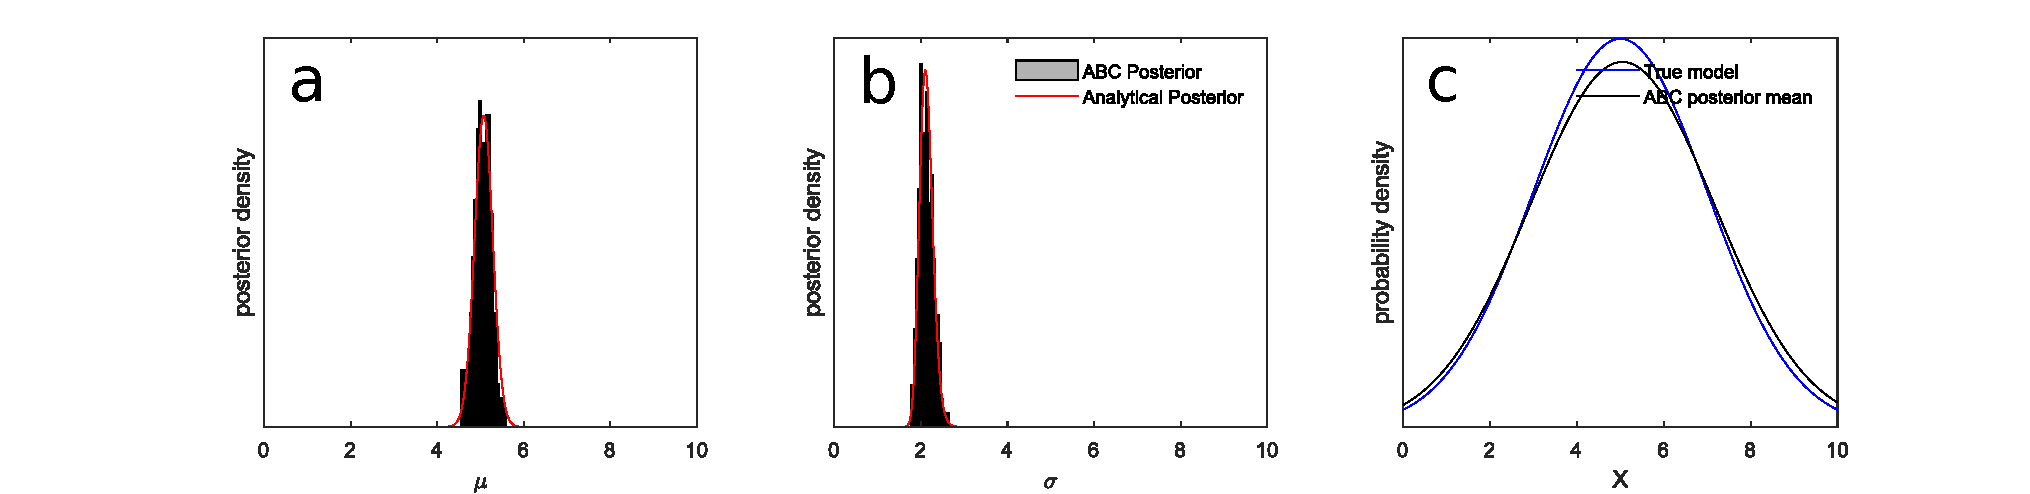
\includegraphics[scale=0.45]{toy1-fig1.pdf}
	\caption{Posterior comparison between ABC and traditional likelihood inference for estimating the parameters, $\bm{\theta} = [\mu,\sigma]$, to a Gaussian model given $n = 100$ observations, $\bm{y}$. The ABC algorithm, algorithm \ref{ABCrejectionsampler}, uses 1 million repititions and a tolerance $\epsilon = 0.1$. The likelihood takes the form $\mathcal{L}(\bm{\theta}|\bm{Y}) = (2\pi\sigma^2)^{-n/2}\ \text{exp}\big[-\frac{1}{2\sigma^2}\sum_{i = 1}^{n}(y_i-\mu)^2\big]$. (a) Marginal posterior compared to marginal ABC posterior for unknown parameter $\mu$. (b) same as (a) but for unknown parameter $\sigma$. (c) Mean ABC posterior model compared to true model.}
	\label{toy1-fig1}
\end{figure}

\begin{figure}[H]
	\centering
	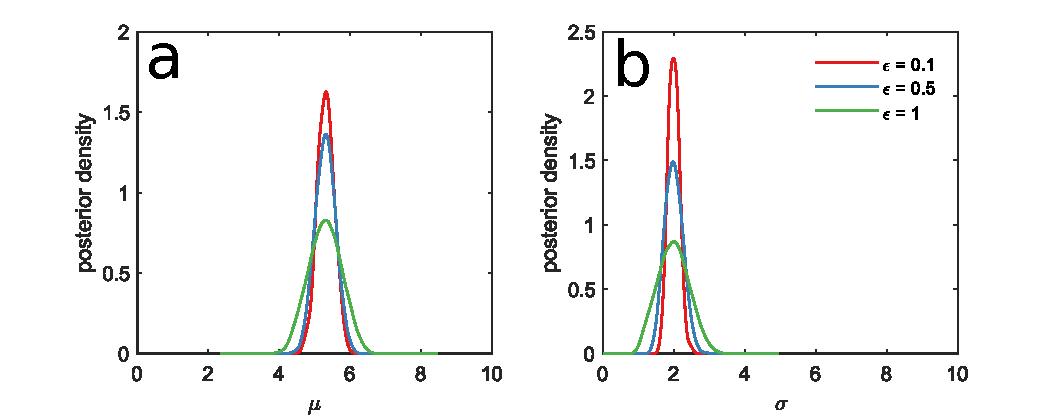
\includegraphics[scale=0.6]{toy1-fig2.pdf}
	\caption{The effect of varying the tolerance $\epsilon$ when estimating $\bm{\theta} = [\mu,\sigma]$ to a Gaussian model given given $n = 100$ observations, $\bm{y}$. Three tolerances are considered, $\epsilon = 0.1$, $\epsilon = 0.5$, $\epsilon = 1$. (a) Marginal ABC posterior for unknown parameter $\mu$. The true value is $\mu = 5$ (b) same as (a) but for unknown parameter $\sigma$. The true value is $\sigma = 2$}.
	\label{toy1-fig2}
\end{figure}

Figure \ref{toy1-fig1} demonstrates that with sufficient statistics and a low tolerance ABC can accurately resolve the posterior using only the ability to simulate data. However, as figure \ref{toy1-fig2} demonstrates, high tolerances erode posterior accuracy and uncertainty is over-estimated. However, it is true that increasing the tolerance increases the acceptance rate and hence relaxes computational resources. In this case the acceptance rate with $\epsilon = 0.1$ was $0.021\%$, while the acceptance rate with $\epsilon = 1$ was $2.023\%$. Under a model which is expensive to simulate from, walking the tightrope between accuracy and efficiency becomes important and needs to be carefully examined. In spite of shortcomings, the strengths of the ABC rejection sampler has led to significant scientific experiments \citep{Fu1997,Weiss1998a,Pritchard1999a}.

\section{Toy problem 2: Linear regression}
\label{sec-lin-reg}

As a second example consider we have observed some data, $\bm{y}$, from the linear model $\bm{g}(\bm{\theta}) = m\bm{x} + b$ and there is some stochasticity in the measurement process such that $\bm{g_s}(\bm{\theta}) = \bm{g}(\bm{\theta}) + \mathcal{N}(0,\sigma^2)$. Our unknown parameters are $\bm{\theta} = [m,b]$, while $\sigma$ is known. In this case it is deemed that computational resources are limitied and MCMC, which uses local transitions, will be needed to improve acceptance rates. MCMC will also be needed when the search spaces are high dimensional, with many unknown parameters, or the posterior is a long way from the prior. For this case we can call upon ABC-MCMC in the form of algorithm \ref{ABC-MCMC}. \\

Algorithm \ref{ABC-MCMC} samples the ABC posterior, equation \ref{summary-stat-abc-posterior}. The algorithm relies on evaluating the MH acceptance probability, equation \ref{M-H-acce}. In our implementations Gaussian proposal distributions, $q(\cdot,\cdot)$, are strictly used. As such the proposal distributions cancel out in equation \ref{M-H-acce}. That leaves the prior and the weighting kernel to be evalutated at each time step in the Markov chain. The weighting kernel takes the form of equation \ref{generic-weighting-kernel}. In this case a uniform weighting kernel, $K_U$, is implemented. The interpretation of $K_U$ is the same as the accept/reject step in the rejection sampler: 
\begin{equation}
	K_U = 
	\begin{cases}
		1 & \text{if}\ 	\frac{\text{d}(S_i(\bm{y^*}),S_i(\bm{y}))}				{\epsilon_i} \leq 1\\
		0 & \text{if}\ \frac{\text{d}(S_i(\bm{y^*}) - S_i(\bm{y}))}				{\epsilon_i} > 1
	\end{cases}
\end{equation}
$K_U$ hence forms an indicator function $\mathbbm{1}$ which is equal to $1$ when the distance between statistics, which are fit marginally, is less than the tolerance. Given, $\bm{S} = \{S_1,\dots,S_O\}$, the weighting kernel takes the form:
\begin{equation}
	p(\bm{S}(\bm{y})|\bm{S}(\bm{y^*}),\bm{\theta}) = \prod_{i = 1}^{O} K_U\Big(\frac{\text{d}(S_i(\bm{y}),S_i(\bm{y^*})}{\epsilon_i}\Big)
	\label{weight-kernel}
\end{equation}
\noindent
As with the 1D Gaussian example it would be possible to take summaries which have a 1:1 correspondance to the unknown parameters. For a given simulation, a linear model could be fit to the simulated data. The slope and intercept of the fit model could then be used as summaries. However, to demonstrate that this is not necessary, we take inspiration from \citet{vrugt2013toward} and use sample mean, $\bar{\mu}$, and sample standard deviation, $\bar{\sigma}$, as summary statistics. The slope is restricted to a positive value to make these statistics sufficient. \\

Figure \ref{linear-regression} shows ABC-MCMC applied to the linear regression problem. \\

In the next section we continue to introduce algorithmic considerations into ABC as we build toward a geophysically relevant parameter estimation system. \\

%\begin{figure}[H]
%	\centering
%	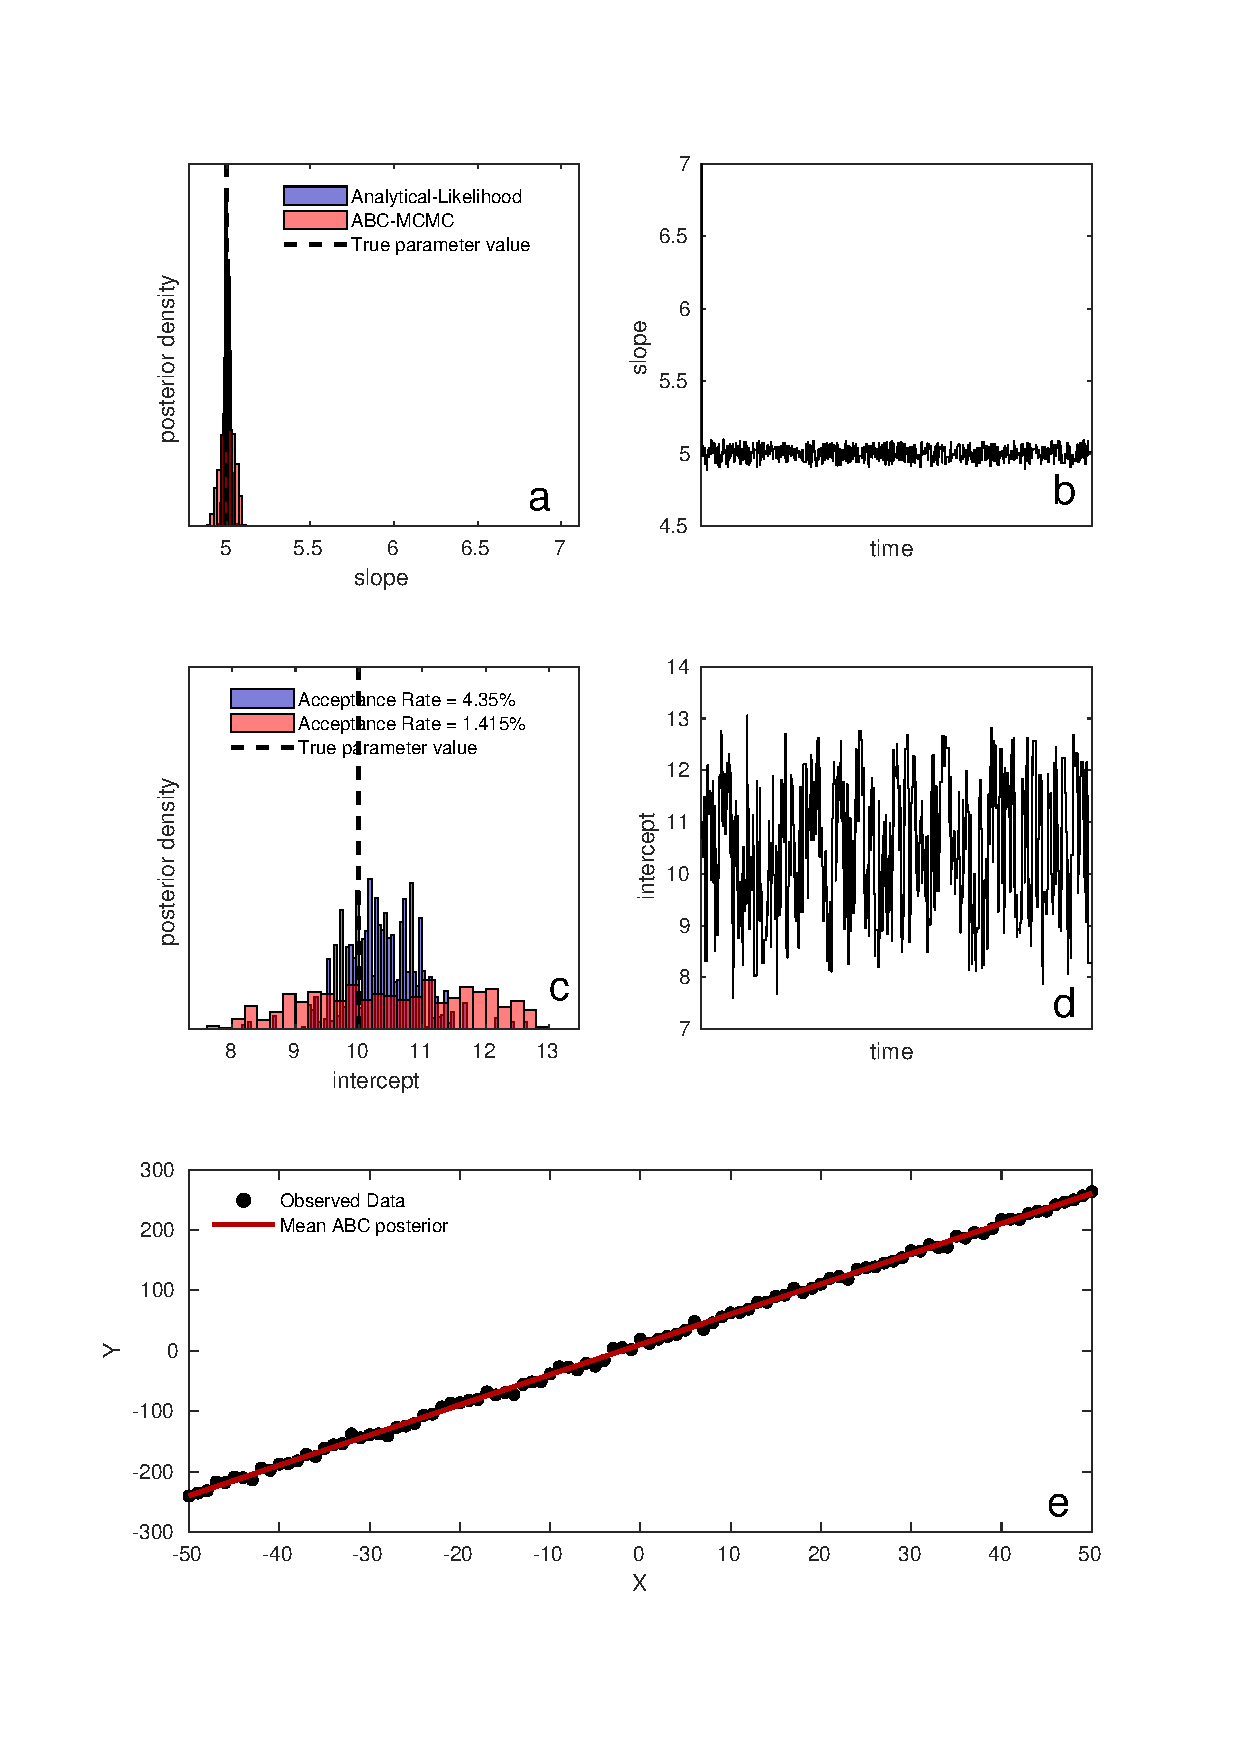
\includegraphics[scale=0.7]{linear-regression.pdf}
%	\caption{Linear regression with ABC. The ABC posterior is also compared to traditional likelihood inference. MCMC is used to sample both posteriors. For ABC the tolerance is $\epsilon = [2\ 2]$. The proposal distribution is $q = \mathcal{N}([0,0],I)$. The Markov chain length is $20\ 000$. (a) The marginal ABC posterior and marginal analytical posterior compared for unknown parameter $m$. (b) Plot of the ABC-MCMC Markov chain through time for $m$. (c) Same as (a) except for unknown parameter $b$. (d) Same as (b) except for unknown parameter $b$. (e) Comparison of the mean ABC posterior model and the observed data generated with $m = 5$, $b = 10$ and $\sigma = 5$.}
%	\label{linear-regression}
%\end{figure}
\begin{figure}[H]	
	\centering
	
	\setlength\fheight{1\linewidth}
	\setlength\fwidth{0.8\linewidth}
	
	%\input{./scattertest.tex}
	% This file was created by matlab2tikz.
%
%The latest updates can be retrieved from
%  http://www.mathworks.com/matlabcentral/fileexchange/22022-matlab2tikz-matlab2tikz
%where you can also make suggestions and rate matlab2tikz.
%
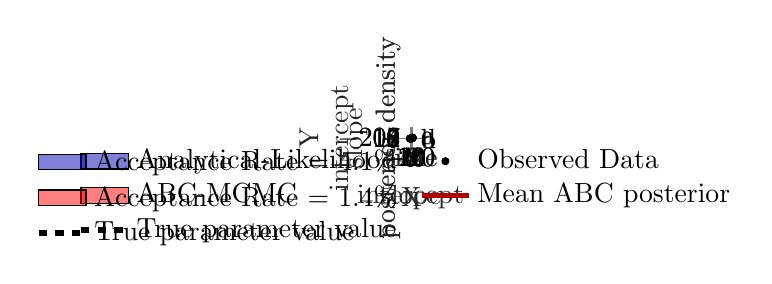
\begin{tikzpicture}

\begin{axis}[%
width=0.411\fwidth,
height=0.265\fheight,
at={(0\fwidth,0.735\fheight)},
scale only axis,
clip=false,
xmin=4.55245,
xmax=7.11655,
xlabel style={font=\color{white!15!black}},
xlabel={slope},
ymin=0,
ymax=30,
ytick={\empty},
ylabel style={font=\color{white!15!black}},
ylabel={posterior density},
axis background/.style={fill=white},
legend style={legend cell align=left, align=left, fill=none, draw=none}
]
\addplot[ybar interval, fill=black!30!blue, fill opacity=0.5, draw=black, area legend] table[row sep=crcr] {%
x	y\\
4.669	0.045045045045046\\
4.67677	0\\
4.68454	0\\
4.69231	0\\
4.70008	0.00643500643500657\\
4.70785	0\\
4.71562	0\\
4.72339	0\\
4.73116	0\\
4.73893	0\\
4.7467	0\\
4.75447	0\\
4.76224	0\\
4.77001	0\\
4.77778	0\\
4.78555	0\\
4.79332	0\\
4.80109	0\\
4.80886	0\\
4.81663	0\\
4.8244	0\\
4.83217	0\\
4.83994	0\\
4.84771	0\\
4.85548	0\\
4.86325	0\\
4.87102	0\\
4.87879	0.090090090090092\\
4.88656	0\\
4.89433	0.00643500643500584\\
4.9021	0\\
4.90987	0.296010296010302\\
4.91764	0.405405405405414\\
4.92541	2.12355212355217\\
4.93318	3.68725868725834\\
4.94095	6.38352638352652\\
4.94872	16.4285714285718\\
4.95649	28.2818532818539\\
4.96426	20.8301158301163\\
4.97203	17.1814671814656\\
4.9798	11.4478764478767\\
4.98757	8.50707850707869\\
4.99534	8.79021879021898\\
5.00311	2.62548262548268\\
5.01088	0.894465894465914\\
5.01865	0.559845559845508\\
5.02642	0\\
5.03419	0\\
5.04196	0\\
5.04973	0\\
5.0575	0\\
5.06527	0\\
5.07304	0\\
5.08081	0\\
5.08858	0\\
5.09635	0\\
5.10412	0\\
5.11189	0\\
5.11966	0\\
5.12743	0\\
5.1352	0\\
5.14297	0\\
5.15074	0\\
5.15851	0\\
5.16628	0\\
5.17405	0\\
5.18182	0\\
5.18959	0\\
5.19736	0\\
5.20513	0\\
5.2129	0\\
5.22067	0\\
5.22844	0\\
5.23621	0\\
5.24398	0\\
5.25175	0\\
5.25952	0\\
5.26729	0\\
5.27506	0\\
5.28283	0\\
5.2906	0\\
5.29837	0\\
5.30614	0\\
5.31391	0\\
5.32168	0\\
5.32945	0\\
5.33722	0\\
5.34499	0\\
5.35276	0\\
5.36053	0\\
5.3683	0.0257400257400263\\
5.37607	0\\
5.38384	0\\
5.39161	0\\
5.39938	0\\
5.40715	0\\
5.41492	0\\
5.42269	0\\
5.43046	0\\
5.43823	0\\
5.446	0\\
5.45377	0\\
5.46154	0\\
5.46931	0\\
5.47708	0\\
5.48485	0\\
5.49262	0\\
5.50039	0\\
5.50816	0\\
5.51593	0.045045045045046\\
5.5237	0\\
5.53147	0\\
5.53924	0\\
5.54701	0.0128700128700131\\
5.55478	0\\
5.56255	0\\
5.57032	0\\
5.57809	0\\
5.58586	0\\
5.59363	0\\
5.6014	0\\
5.60917	0\\
5.61694	0\\
5.62471	0\\
5.63248	0\\
5.64025	0\\
5.64802	0\\
5.65579	0\\
5.66356	0\\
5.67133	0\\
5.6791	0\\
5.68687	0\\
5.69464	0\\
5.70241	0\\
5.71018	0\\
5.71795	0\\
5.72572	0\\
5.73349	0\\
5.74126	0\\
5.74903	0\\
5.7568	0\\
5.76457	0\\
5.77234	0\\
5.78011	0\\
5.78788	0\\
5.79565	0\\
5.80342	0\\
5.81119	0\\
5.81896	0\\
5.82673	0\\
5.8345	0\\
5.84227	0\\
5.85004	0\\
5.85781	0\\
5.86558	0\\
5.87335	0\\
5.88112	0\\
5.88889	0\\
5.89666	0\\
5.90443	0\\
5.9122	0\\
5.91997	0\\
5.92774	0\\
5.93551	0\\
5.94328	0\\
5.95105	0\\
5.95882	0\\
5.96659	0\\
5.97436	0\\
5.98213	0\\
5.9899	0\\
5.99767	0\\
6.00544	0\\
6.01321	0\\
6.02098	0\\
6.02875	0\\
6.03652	0\\
6.04429	0\\
6.05206	0\\
6.05983	0\\
6.0676	0\\
6.07537	0\\
6.08314	0\\
6.09091	0\\
6.09868	0\\
6.10645	0\\
6.11422	0\\
6.12199	0\\
6.12976	0\\
6.13753	0\\
6.1453	0\\
6.15307	0\\
6.16084	0\\
6.16861	0\\
6.17638	0\\
6.18415	0\\
6.19192	0\\
6.19969	0\\
6.20746	0\\
6.21523	0\\
6.223	0\\
6.23077	0\\
6.23854	0\\
6.24631	0\\
6.25408	0\\
6.26185	0\\
6.26962	0\\
6.27739	0\\
6.28516	0\\
6.29293	0\\
6.3007	0\\
6.30847	0\\
6.31624	0\\
6.32401	0\\
6.33178	0\\
6.33955	0\\
6.34732	0\\
6.35509	0\\
6.36286	0\\
6.37063	0\\
6.3784	0\\
6.38617	0\\
6.39394	0\\
6.40171	0\\
6.40948	0\\
6.41725	0\\
6.42502	0\\
6.43279	0\\
6.44056	0\\
6.44833	0\\
6.4561	0\\
6.46387	0\\
6.47164	0\\
6.47941	0\\
6.48718	0\\
6.49495	0\\
6.50272	0\\
6.51049	0\\
6.51826	0\\
6.52603	0\\
6.5338	0\\
6.54157	0\\
6.54934	0\\
6.55711	0\\
6.56488	0\\
6.57265	0\\
6.58042	0\\
6.58819	0\\
6.59596	0\\
6.60373	0\\
6.6115	0\\
6.61927	0\\
6.62704	0\\
6.63481	0\\
6.64258	0\\
6.65035	0\\
6.65812	0\\
6.66589	0\\
6.67366	0\\
6.68143	0\\
6.6892	0\\
6.69697	0.0193050193050197\\
6.70474	0\\
6.71251	0\\
6.72028	0\\
6.72805	0\\
6.73582	0\\
6.74359	0\\
6.75136	0\\
6.75913	0\\
6.7669	0\\
6.77467	0\\
6.78244	0\\
6.79021	0\\
6.79798	0\\
6.80575	0\\
6.81352	0\\
6.82129	0\\
6.82906	0\\
6.83683	0\\
6.8446	0\\
6.85237	0\\
6.86014	0\\
6.86791	0\\
6.87568	0\\
6.88345	0\\
6.89122	0\\
6.89899	0\\
6.90676	0\\
6.91453	0\\
6.9223	0\\
6.93007	0\\
6.93784	0\\
6.94561	0\\
6.95338	0\\
6.96115	0\\
6.96892	0\\
6.97669	0\\
6.98446	0\\
6.99223	0.00643500643500657\\
7	0.00643500643500657\\
};
\addlegendentry{Analytical-Likelihood}

\addplot[ybar interval, fill=red, fill opacity=0.5, draw=black, area legend] table[row sep=crcr] {%
x	y\\
4.86	0.532710280373835\\
4.8814	2.61915887850469\\
4.9028	6.45327102803742\\
4.9242	6.16121495327081\\
4.9456	7.45794392523369\\
4.967	8.03271028037388\\
4.9884	6.035046728972\\
5.0098	5.85046728971966\\
5.0312	2.75467289719628\\
5.0526	0.313084112149522\\
5.074	0\\
5.0954	0\\
5.1168	0\\
5.1382	0\\
5.1596	0\\
5.181	0\\
5.2024	0\\
5.2238	0\\
5.2452	0\\
5.2666	0\\
5.288	0\\
5.3094	0\\
5.3308	0\\
5.3522	0\\
5.3736	0\\
5.395	0\\
5.4164	0\\
5.4378	0\\
5.4592	0\\
5.4806	0\\
5.502	0\\
5.5234	0\\
5.5448	0\\
5.5662	0\\
5.5876	0\\
5.609	0\\
5.6304	0\\
5.6518	0\\
5.6732	0\\
5.6946	0\\
5.716	0\\
5.7374	0\\
5.7588	0\\
5.7802	0\\
5.8016	0\\
5.823	0\\
5.8444	0\\
5.8658	0\\
5.8872	0\\
5.9086	0\\
5.93	0\\
5.9514	0\\
5.9728	0\\
5.9942	0\\
6.0156	0\\
6.037	0\\
6.0584	0\\
6.0798	0\\
6.1012	0\\
6.1226	0\\
6.144	0\\
6.1654	0\\
6.1868	0\\
6.2082	0\\
6.2296	0\\
6.251	0\\
6.2724	0\\
6.2938	0\\
6.3152	0\\
6.3366	0\\
6.358	0\\
6.3794	0\\
6.4008	0\\
6.4222	0\\
6.4436	0\\
6.465	0\\
6.4864	0\\
6.5078	0\\
6.5292	0\\
6.5506	0\\
6.572	0\\
6.5934	0\\
6.6148	0\\
6.6362	0\\
6.6576	0\\
6.679	0\\
6.7004	0\\
6.7218	0\\
6.7432	0\\
6.7646	0\\
6.786	0\\
6.8074	0\\
6.8288	0\\
6.8502	0\\
6.8716	0\\
6.893	0\\
6.9144	0\\
6.9358	0\\
6.9572	0\\
6.9786	0.51869158878505\\
7	0.51869158878505\\
};
\addlegendentry{ABC-MCMC}

\addplot [color=black, dashed, line width=2.0pt]
  table[row sep=crcr]{%
5	0\\
5	0.303030303030303\\
5	0.606060606060606\\
5	0.909090909090909\\
5	1.21212121212121\\
5	1.51515151515152\\
5	1.81818181818182\\
5	2.12121212121212\\
5	2.42424242424242\\
5	2.72727272727273\\
5	3.03030303030303\\
5	3.33333333333333\\
5	3.63636363636364\\
5	3.93939393939394\\
5	4.24242424242424\\
5	4.54545454545455\\
5	4.84848484848485\\
5	5.15151515151515\\
5	5.45454545454545\\
5	5.75757575757576\\
5	6.06060606060606\\
5	6.36363636363636\\
5	6.66666666666667\\
5	6.96969696969697\\
5	7.27272727272727\\
5	7.57575757575758\\
5	7.87878787878788\\
5	8.18181818181818\\
5	8.48484848484848\\
5	8.78787878787879\\
5	9.09090909090909\\
5	9.39393939393939\\
5	9.6969696969697\\
5	10\\
5	10.3030303030303\\
5	10.6060606060606\\
5	10.9090909090909\\
5	11.2121212121212\\
5	11.5151515151515\\
5	11.8181818181818\\
5	12.1212121212121\\
5	12.4242424242424\\
5	12.7272727272727\\
5	13.030303030303\\
5	13.3333333333333\\
5	13.6363636363636\\
5	13.9393939393939\\
5	14.2424242424242\\
5	14.5454545454545\\
5	14.8484848484848\\
5	15.1515151515152\\
5	15.4545454545455\\
5	15.7575757575758\\
5	16.0606060606061\\
5	16.3636363636364\\
5	16.6666666666667\\
5	16.969696969697\\
5	17.2727272727273\\
5	17.5757575757576\\
5	17.8787878787879\\
5	18.1818181818182\\
5	18.4848484848485\\
5	18.7878787878788\\
5	19.0909090909091\\
5	19.3939393939394\\
5	19.6969696969697\\
5	20\\
5	20.3030303030303\\
5	20.6060606060606\\
5	20.9090909090909\\
5	21.2121212121212\\
5	21.5151515151515\\
5	21.8181818181818\\
5	22.1212121212121\\
5	22.4242424242424\\
5	22.7272727272727\\
5	23.030303030303\\
5	23.3333333333333\\
5	23.6363636363636\\
5	23.9393939393939\\
5	24.2424242424242\\
5	24.5454545454545\\
5	24.8484848484848\\
5	25.1515151515152\\
5	25.4545454545455\\
5	25.7575757575758\\
5	26.0606060606061\\
5	26.3636363636364\\
5	26.6666666666667\\
5	26.969696969697\\
5	27.2727272727273\\
5	27.5757575757576\\
5	27.8787878787879\\
5	28.1818181818182\\
5	28.4848484848485\\
5	28.7878787878788\\
5	29.0909090909091\\
5	29.3939393939394\\
5	29.6969696969697\\
5	30\\
};
\addlegendentry{True parameter value}

\node[right, align=left]
at (rel axis cs:0.9,0.1) {a};
\end{axis}

\begin{axis}[%
width=0.411\fwidth,
height=0.265\fheight,
at={(0.54\fwidth,0.735\fheight)},
scale only axis,
clip=false,
xmin=0,
xmax=20000,
xtick={\empty},
xlabel style={font=\color{white!15!black}},
xlabel={time},
ymin=4,
ymax=7,
ylabel style={font=\color{white!15!black}},
ylabel={slope},
axis background/.style={fill=white},
legend style={legend cell align=left, align=left, draw=white!15!black}
]
\addplot [color=black, forget plot]
  table[row sep=crcr]{%
1	7\\
3	7\\
5	7\\
7	7\\
9	7\\
11	7\\
13	7\\
15	7\\
17	7\\
19	7\\
21	7\\
23	7\\
25	7\\
27	7\\
29	7\\
31	7\\
33	7\\
35	7\\
37	7\\
39	7\\
41	7\\
43	7\\
45	7\\
47	7\\
49	7\\
51	7\\
53	7\\
55	7\\
57	7\\
59	7\\
61	7\\
63	7\\
65	7\\
67	7\\
69	7\\
71	7\\
73	7\\
75	7\\
77	7\\
79	7\\
81	7\\
83	7\\
85	7\\
87	7\\
89	7\\
91	7\\
93	7\\
95	7\\
97	7\\
99	7\\
101	7\\
103	7\\
105	7\\
107	7\\
109	7\\
111	7\\
113	7\\
115	7\\
117	7\\
119	7\\
121	7\\
123	7\\
125	7\\
127	7\\
129	7\\
131	7\\
133	7\\
135	7\\
137	7\\
139	7\\
141	7\\
143	7\\
145	7\\
147	7\\
149	7\\
151	7\\
153	7\\
155	7\\
157	7\\
159	7\\
161	7\\
163	7\\
165	7\\
167	7\\
169	7\\
171	7\\
173	7\\
175	7\\
177	7\\
179	7\\
181	7\\
183	7\\
185	7\\
187	7\\
189	7\\
191	7\\
193	7\\
195	7\\
197	7\\
199	7\\
201	7\\
203	7\\
205	7\\
207	7\\
209	7\\
211	7\\
213	7\\
215	7\\
217	7\\
219	7\\
221	7\\
223	4.95785141119881\\
225	4.95785141119881\\
227	4.96999655845837\\
229	4.96999655845837\\
231	4.96999655845837\\
233	4.96999655845837\\
235	4.98239856213861\\
237	4.98239856213861\\
239	4.98239856213861\\
241	4.98239856213861\\
243	4.98239856213861\\
245	4.98239856213861\\
247	4.98239856213861\\
249	4.98239856213861\\
251	4.98239856213861\\
253	4.98239856213861\\
255	4.98239856213861\\
257	4.98239856213861\\
259	4.98239856213861\\
261	4.98239856213861\\
263	4.98239856213861\\
265	4.98239856213861\\
267	4.98239856213861\\
269	4.98239856213861\\
271	4.98239856213861\\
273	4.98239856213861\\
275	4.98239856213861\\
277	4.98239856213861\\
279	4.98239856213861\\
281	4.98239856213861\\
283	5.0146829825097\\
285	5.0146829825097\\
287	4.94877850713173\\
289	4.94877850713173\\
291	4.94877850713173\\
293	4.94877850713173\\
295	4.94877850713173\\
297	4.94877850713173\\
299	4.89771303038766\\
301	4.89771303038766\\
303	4.89771303038766\\
305	4.89771303038766\\
307	4.89771303038766\\
309	4.95102911686232\\
311	4.95102911686232\\
313	4.95102911686232\\
315	4.95102911686232\\
317	4.95102911686232\\
319	4.95102911686232\\
321	4.95102911686232\\
323	4.95102911686232\\
325	4.95102911686232\\
327	4.95102911686232\\
329	4.95102911686232\\
331	4.95102911686232\\
333	4.95102911686232\\
335	4.95102911686232\\
337	4.95102911686232\\
339	4.95102911686232\\
341	4.95102911686232\\
343	4.95522086070316\\
345	4.95522086070316\\
347	4.95522086070316\\
349	4.95522086070316\\
351	4.95522086070316\\
353	4.95522086070316\\
355	4.95522086070316\\
357	4.95522086070316\\
359	4.95522086070316\\
361	4.95522086070316\\
363	4.95522086070316\\
365	4.95522086070316\\
367	4.95522086070316\\
369	4.95522086070316\\
371	4.95522086070316\\
373	4.95522086070316\\
375	4.95522086070316\\
377	4.95522086070316\\
379	4.95522086070316\\
381	4.95522086070316\\
383	4.95522086070316\\
385	4.95522086070316\\
387	4.95522086070316\\
389	4.95522086070316\\
391	4.95522086070316\\
393	4.95288426466109\\
395	4.99164486003855\\
397	4.95117513065989\\
399	4.95117513065989\\
401	4.95117513065989\\
403	4.95117513065989\\
405	4.95251065052736\\
407	4.95251065052736\\
409	4.95251065052736\\
411	4.95251065052736\\
413	4.95251065052736\\
415	4.9766892525467\\
417	4.9766892525467\\
419	4.9766892525467\\
421	4.96970957622483\\
423	4.96970957622483\\
425	4.96970957622483\\
427	4.96970957622483\\
429	4.96970957622483\\
431	4.96970957622483\\
433	4.96970957622483\\
435	4.96970957622483\\
437	4.96970957622483\\
439	4.96970957622483\\
441	4.96970957622483\\
443	4.96970957622483\\
445	4.96970957622483\\
447	4.96970957622483\\
449	4.96970957622483\\
451	4.96970957622483\\
453	4.96970957622483\\
455	4.96970957622483\\
457	4.96970957622483\\
459	4.96970957622483\\
461	4.96970957622483\\
463	4.96970957622483\\
465	4.96970957622483\\
467	4.96970957622483\\
469	4.96970957622483\\
471	4.96970957622483\\
473	4.96970957622483\\
475	4.96970957622483\\
477	4.96970957622483\\
479	5.02821676964716\\
481	5.02821676964716\\
483	4.94785000897964\\
485	4.94785000897964\\
487	4.94785000897964\\
489	4.94785000897964\\
491	4.94785000897964\\
493	4.94785000897964\\
495	4.94785000897964\\
497	4.90422520040274\\
499	4.90422520040274\\
501	4.90422520040274\\
503	4.90422520040274\\
505	4.90422520040274\\
507	4.90422520040274\\
509	4.90422520040274\\
511	4.90422520040274\\
513	4.90422520040274\\
515	4.90422520040274\\
517	4.90422520040274\\
519	4.90422520040274\\
521	4.9521559148432\\
523	4.9521559148432\\
525	4.9521559148432\\
527	4.9521559148432\\
529	4.9521559148432\\
531	4.9521559148432\\
533	4.9521559148432\\
535	4.9521559148432\\
537	4.9521559148432\\
539	4.9521559148432\\
541	4.9521559148432\\
543	4.9521559148432\\
545	4.9521559148432\\
547	4.9521559148432\\
549	4.9491921909415\\
551	4.9491921909415\\
553	4.9491921909415\\
555	4.9491921909415\\
557	4.9491921909415\\
559	4.9491921909415\\
561	4.9491921909415\\
563	4.9491921909415\\
565	4.9491921909415\\
567	4.9491921909415\\
569	4.9491921909415\\
571	4.9491921909415\\
573	4.9491921909415\\
575	4.9491921909415\\
577	4.99199334641703\\
579	4.99199334641703\\
581	4.99199334641703\\
583	4.99199334641703\\
585	4.99199334641703\\
587	4.99199334641703\\
589	4.99199334641703\\
591	4.99199334641703\\
593	4.99199334641703\\
595	4.99199334641703\\
597	4.942463400871\\
599	4.942463400871\\
601	4.942463400871\\
603	4.942463400871\\
605	4.942463400871\\
607	4.942463400871\\
609	4.942463400871\\
611	4.942463400871\\
613	4.942463400871\\
615	4.942463400871\\
617	4.942463400871\\
619	4.942463400871\\
621	4.942463400871\\
623	4.942463400871\\
625	4.942463400871\\
627	4.942463400871\\
629	4.942463400871\\
631	4.942463400871\\
633	4.9604356801294\\
635	4.9604356801294\\
637	4.9604356801294\\
639	4.9604356801294\\
641	4.9604356801294\\
643	4.9604356801294\\
645	4.9604356801294\\
647	4.9604356801294\\
649	4.9604356801294\\
651	4.9604356801294\\
653	4.9604356801294\\
655	4.9604356801294\\
657	4.97071188465244\\
659	4.97071188465244\\
661	4.97071188465244\\
663	4.97071188465244\\
665	4.97071188465244\\
667	4.92049952463755\\
669	4.92049952463755\\
671	4.96135581976622\\
673	4.96135581976622\\
675	4.96135581976622\\
677	4.96135581976622\\
679	4.96135581976622\\
681	4.96135581976622\\
683	4.95307179496519\\
685	4.95307179496519\\
687	4.95307179496519\\
689	4.95307179496519\\
691	4.95307179496519\\
693	4.95307179496519\\
695	4.95307179496519\\
697	4.95307179496519\\
699	4.95307179496519\\
701	4.97815062455302\\
703	4.97815062455302\\
705	4.97815062455302\\
707	4.97815062455302\\
709	4.97815062455302\\
711	4.97815062455302\\
713	4.97815062455302\\
715	4.97815062455302\\
717	4.97815062455302\\
719	4.97815062455302\\
721	4.97815062455302\\
723	4.97815062455302\\
725	4.97815062455302\\
727	4.97815062455302\\
729	5.02549935843886\\
731	5.02549935843886\\
733	5.02549935843886\\
735	5.02549935843886\\
737	5.02549935843886\\
739	5.02549935843886\\
741	5.02549935843886\\
743	5.02549935843886\\
745	5.02549935843886\\
747	5.02549935843886\\
749	5.02549935843886\\
751	5.02549935843886\\
753	4.91656476030246\\
755	4.91656476030246\\
757	4.91656476030246\\
759	4.91656476030246\\
761	4.91656476030246\\
763	4.91656476030246\\
765	4.91656476030246\\
767	4.91656476030246\\
769	4.91656476030246\\
771	4.91656476030246\\
773	4.91656476030246\\
775	4.91656476030246\\
777	4.91656476030246\\
779	4.97644681733332\\
781	4.97644681733332\\
783	4.97644681733332\\
785	4.97644681733332\\
787	4.97644681733332\\
789	4.97644681733332\\
791	4.97644681733332\\
793	4.97644681733332\\
795	4.97644681733332\\
797	4.97644681733332\\
799	4.97644681733332\\
801	4.97644681733332\\
803	4.97644681733332\\
805	4.97644681733332\\
807	4.97644681733332\\
809	4.97644681733332\\
811	4.97644681733332\\
813	4.97644681733332\\
815	4.97644681733332\\
817	4.97644681733332\\
819	4.97644681733332\\
821	4.97644681733332\\
823	4.91034973708328\\
825	4.91034973708328\\
827	4.91034973708328\\
829	4.91034973708328\\
831	4.91034973708328\\
833	4.97833340739734\\
835	4.97833340739734\\
837	4.97833340739734\\
839	4.97833340739734\\
841	4.97833340739734\\
843	4.97833340739734\\
845	4.97833340739734\\
847	4.97833340739734\\
849	4.97833340739734\\
851	4.97833340739734\\
853	4.97833340739734\\
855	4.97833340739734\\
857	4.97833340739734\\
859	4.99509266472277\\
861	5.02710212636354\\
863	4.9504662145773\\
865	4.9504662145773\\
867	4.94618353643547\\
869	4.94618353643547\\
871	4.94618353643547\\
873	4.94618353643547\\
875	4.97043636988937\\
877	4.97043636988937\\
879	4.97043636988937\\
881	4.97043636988937\\
883	4.97043636988937\\
885	4.97043636988937\\
887	4.97043636988937\\
889	4.97043636988937\\
891	4.97043636988937\\
893	4.97043636988937\\
895	4.97043636988937\\
897	4.97043636988937\\
899	4.97043636988937\\
901	4.97043636988937\\
903	4.97043636988937\\
905	4.97043636988937\\
907	4.97043636988937\\
909	4.97043636988937\\
911	4.953348894624\\
913	4.953348894624\\
915	4.953348894624\\
917	4.953348894624\\
919	4.953348894624\\
921	4.953348894624\\
923	4.953348894624\\
925	4.97905217729531\\
927	4.97905217729531\\
929	4.97905217729531\\
931	4.97905217729531\\
933	4.97905217729531\\
935	4.97905217729531\\
937	4.97905217729531\\
939	4.97905217729531\\
941	4.97905217729531\\
943	4.97905217729531\\
945	4.97905217729531\\
947	4.97905217729531\\
949	4.97905217729531\\
951	4.97905217729531\\
953	4.97905217729531\\
955	4.96282756920545\\
957	4.96282756920545\\
959	4.96282756920545\\
961	4.97271443233739\\
963	4.97271443233739\\
965	4.97271443233739\\
967	4.97271443233739\\
969	4.97271443233739\\
971	4.97271443233739\\
973	4.97271443233739\\
975	4.91476777946059\\
977	4.91476777946059\\
979	4.91476777946059\\
981	4.91896689211257\\
983	4.91896689211257\\
985	4.91896689211257\\
987	4.91896689211257\\
989	4.91896689211257\\
991	4.91896689211257\\
993	4.91896689211257\\
995	4.91896689211257\\
997	4.91896689211257\\
999	4.91896689211257\\
1001	4.91896689211257\\
1003	4.91896689211257\\
1005	4.91896689211257\\
1007	4.91896689211257\\
1009	4.91896689211257\\
1011	4.95575295468091\\
1013	4.95575295468091\\
1015	4.95575295468091\\
1017	4.95575295468091\\
1019	4.95575295468091\\
1021	4.95575295468091\\
1023	4.95575295468091\\
1025	4.95575295468091\\
1027	4.95575295468091\\
1029	4.95575295468091\\
1031	4.95575295468091\\
1033	4.95575295468091\\
1035	4.95575295468091\\
1037	4.95575295468091\\
1039	4.95575295468091\\
1041	4.95575295468091\\
1043	4.95575295468091\\
1045	4.95575295468091\\
1047	4.98546822109754\\
1049	4.98546822109754\\
1051	4.98546822109754\\
1053	4.98546822109754\\
1055	4.98546822109754\\
1057	4.98546822109754\\
1059	4.98546822109754\\
1061	4.98546822109754\\
1063	4.92636444117721\\
1065	4.92636444117721\\
1067	4.92636444117721\\
1069	4.92636444117721\\
1071	4.92636444117721\\
1073	4.92636444117721\\
1075	4.92636444117721\\
1077	4.92636444117721\\
1079	4.92636444117721\\
1081	4.92636444117721\\
1083	4.92636444117721\\
1085	4.92636444117721\\
1087	4.92636444117721\\
1089	4.92636444117721\\
1091	4.92636444117721\\
1093	4.92636444117721\\
1095	4.92636444117721\\
1097	5.03345156132906\\
1099	4.95475156361861\\
1101	4.95475156361861\\
1103	4.95475156361861\\
1105	4.95475156361861\\
1107	4.95475156361861\\
1109	4.95475156361861\\
1111	4.95475156361861\\
1113	4.95475156361861\\
1115	4.95475156361861\\
1117	4.95475156361861\\
1119	4.95475156361861\\
1121	4.95475156361861\\
1123	4.95475156361861\\
1125	4.95475156361861\\
1127	4.95475156361861\\
1129	4.95475156361861\\
1131	4.95475156361861\\
1133	4.95475156361861\\
1135	4.95475156361861\\
1137	4.95475156361861\\
1139	4.95475156361861\\
1141	4.95475156361861\\
1143	4.95475156361861\\
1145	4.95475156361861\\
1147	4.95475156361861\\
1149	4.95475156361861\\
1151	4.95475156361861\\
1153	4.95475156361861\\
1155	4.95475156361861\\
1157	4.95475156361861\\
1159	4.95475156361861\\
1161	4.95475156361861\\
1163	4.95475156361861\\
1165	4.95475156361861\\
1167	4.95475156361861\\
1169	4.95475156361861\\
1171	4.95475156361861\\
1173	4.95475156361861\\
1175	4.95475156361861\\
1177	4.95475156361861\\
1179	4.95475156361861\\
1181	4.95475156361861\\
1183	4.95475156361861\\
1185	4.95475156361861\\
1187	4.91715990083082\\
1189	4.91715990083082\\
1191	4.91715990083082\\
1193	4.91715990083082\\
1195	4.91715990083082\\
1197	4.91715990083082\\
1199	4.91715990083082\\
1201	4.91715990083082\\
1203	4.91715990083082\\
1205	4.91715990083082\\
1207	4.91715990083082\\
1209	4.91715990083082\\
1211	5.03556165014388\\
1213	5.03556165014388\\
1215	5.03556165014388\\
1217	5.03556165014388\\
1219	5.03556165014388\\
1221	5.03556165014388\\
1223	4.90988977285323\\
1225	4.90988977285323\\
1227	4.90988977285323\\
1229	4.90988977285323\\
1231	4.90988977285323\\
1233	4.90988977285323\\
1235	4.90988977285323\\
1237	4.90988977285323\\
1239	4.90988977285323\\
1241	4.90988977285323\\
1243	4.90988977285323\\
1245	4.90988977285323\\
1247	4.90988977285323\\
1249	4.90988977285323\\
1251	4.90988977285323\\
1253	4.90988977285323\\
1255	4.90988977285323\\
1257	4.90988977285323\\
1259	4.90988977285323\\
1261	4.90988977285323\\
1263	4.90988977285323\\
1265	4.96830336272707\\
1267	4.96830336272707\\
1269	4.96830336272707\\
1271	4.96830336272707\\
1273	4.96830336272707\\
1275	4.96830336272707\\
1277	4.96830336272707\\
1279	4.96830336272707\\
1281	4.96830336272707\\
1283	4.96830336272707\\
1285	4.96830336272707\\
1287	4.95402618220841\\
1289	4.95402618220841\\
1291	4.95402618220841\\
1293	4.95402618220841\\
1295	4.95402618220841\\
1297	4.95402618220841\\
1299	4.95402618220841\\
1301	4.95402618220841\\
1303	4.95402618220841\\
1305	4.9670763271859\\
1307	5.02015461011889\\
1309	5.02015461011889\\
1311	5.02015461011889\\
1313	5.02015461011889\\
1315	5.02015461011889\\
1317	5.02015461011889\\
1319	5.02015461011889\\
1321	5.02015461011889\\
1323	5.02015461011889\\
1325	5.02015461011889\\
1327	5.02015461011889\\
1329	5.02015461011889\\
1331	5.02015461011889\\
1333	5.02015461011889\\
1335	5.02015461011889\\
1337	4.94299867825292\\
1339	4.94299867825292\\
1341	4.94299867825292\\
1343	4.94299867825292\\
1345	4.94299867825292\\
1347	4.94299867825292\\
1349	4.94299867825292\\
1351	4.94299867825292\\
1353	4.94299867825292\\
1355	4.94299867825292\\
1357	4.94299867825292\\
1359	4.94299867825292\\
1361	4.94299867825292\\
1363	4.94299867825292\\
1365	4.94299867825292\\
1367	4.89464368457718\\
1369	4.89464368457718\\
1371	4.89464368457718\\
1373	4.89464368457718\\
1375	4.89464368457718\\
1377	4.89464368457718\\
1379	4.89464368457718\\
1381	4.92749016310727\\
1383	4.92749016310727\\
1385	4.92749016310727\\
1387	4.92749016310727\\
1389	4.92749016310727\\
1391	4.92749016310727\\
1393	4.92749016310727\\
1395	4.92749016310727\\
1397	4.92749016310727\\
1399	4.92749016310727\\
1401	4.92749016310727\\
1403	4.98140899454789\\
1405	4.98140899454789\\
1407	4.98140899454789\\
1409	4.98140899454789\\
1411	4.98140899454789\\
1413	4.90967997567533\\
1415	4.90967997567533\\
1417	4.90967997567533\\
1419	4.90967997567533\\
1421	4.95823298948953\\
1423	4.95823298948953\\
1425	4.95823298948953\\
1427	4.95823298948953\\
1429	4.95823298948953\\
1431	4.95823298948953\\
1433	4.95823298948953\\
1435	4.95823298948953\\
1437	4.95823298948953\\
1439	4.95823298948953\\
1441	5.03596880058105\\
1443	5.03596880058105\\
1445	5.03596880058105\\
1447	5.03596880058105\\
1449	5.03596880058105\\
1451	5.03596880058105\\
1453	5.03596880058105\\
1455	5.03596880058105\\
1457	5.03596880058105\\
1459	5.03596880058105\\
1461	5.03596880058105\\
1463	5.03596880058105\\
1465	5.03596880058105\\
1467	5.03596880058105\\
1469	5.00662837225228\\
1471	5.00662837225228\\
1473	5.00662837225228\\
1475	5.00662837225228\\
1477	4.92755336569996\\
1479	4.92755336569996\\
1481	4.92755336569996\\
1483	4.92755336569996\\
1485	4.92755336569996\\
1487	4.92755336569996\\
1489	4.92755336569996\\
1491	4.92755336569996\\
1493	4.92755336569996\\
1495	4.92755336569996\\
1497	4.92755336569996\\
1499	4.92755336569996\\
1501	4.93328820525489\\
1503	4.93328820525489\\
1505	4.93328820525489\\
1507	4.93328820525489\\
1509	4.93328820525489\\
1511	4.93328820525489\\
1513	4.93328820525489\\
1515	4.93328820525489\\
1517	4.93328820525489\\
1519	4.93328820525489\\
1521	4.93328820525489\\
1523	4.93328820525489\\
1525	4.93328820525489\\
1527	4.93328820525489\\
1529	4.93328820525489\\
1531	4.97410602705107\\
1533	4.97410602705107\\
1535	4.97410602705107\\
1537	4.97410602705107\\
1539	4.97410602705107\\
1541	4.97410602705107\\
1543	4.97410602705107\\
1545	4.97410602705107\\
1547	4.97410602705107\\
1549	4.97410602705107\\
1551	4.97410602705107\\
1553	4.97410602705107\\
1555	4.97410602705107\\
1557	4.97410602705107\\
1559	4.97410602705107\\
1561	4.97410602705107\\
1563	4.97410602705107\\
1565	4.97410602705107\\
1567	4.97410602705107\\
1569	4.97410602705107\\
1571	4.97410602705107\\
1573	4.97410602705107\\
1575	4.92758350699192\\
1577	4.92758350699192\\
1579	4.92758350699192\\
1581	4.92758350699192\\
1583	4.92758350699192\\
1585	4.92758350699192\\
1587	4.92758350699192\\
1589	4.92758350699192\\
1591	4.92758350699192\\
1593	4.92758350699192\\
1595	4.92758350699192\\
1597	4.92758350699192\\
1599	4.92758350699192\\
1601	4.92758350699192\\
1603	4.92758350699192\\
1605	4.92758350699192\\
1607	4.92758350699192\\
1609	4.92758350699192\\
1611	4.92758350699192\\
1613	4.98670334187075\\
1615	4.98670334187075\\
1617	4.98670334187075\\
1619	4.98670334187075\\
1621	4.98670334187075\\
1623	4.98670334187075\\
1625	4.98670334187075\\
1627	4.98670334187075\\
1629	4.98670334187075\\
1631	4.98670334187075\\
1633	4.98670334187075\\
1635	4.98670334187075\\
1637	4.98670334187075\\
1639	4.98670334187075\\
1641	4.98670334187075\\
1643	4.98670334187075\\
1645	4.98670334187075\\
1647	4.98670334187075\\
1649	4.98670334187075\\
1651	4.98670334187075\\
1653	4.98670334187075\\
1655	4.98670334187075\\
1657	4.98670334187075\\
1659	4.98670334187075\\
1661	4.98670334187075\\
1663	4.98670334187075\\
1665	4.98670334187075\\
1667	4.98670334187075\\
1669	4.98670334187075\\
1671	4.98670334187075\\
1673	4.98670334187075\\
1675	4.98670334187075\\
1677	4.8941486919633\\
1679	4.8941486919633\\
1681	4.8941486919633\\
1683	4.8941486919633\\
1685	4.8941486919633\\
1687	4.8941486919633\\
1689	4.8941486919633\\
1691	4.8941486919633\\
1693	4.8941486919633\\
1695	4.95830513187793\\
1697	4.95830513187793\\
1699	4.95830513187793\\
1701	4.95830513187793\\
1703	4.95830513187793\\
1705	4.97485861319841\\
1707	4.97485861319841\\
1709	4.97485861319841\\
1711	4.97485861319841\\
1713	4.97485861319841\\
1715	4.97485861319841\\
1717	4.97485861319841\\
1719	4.97485861319841\\
1721	4.97485861319841\\
1723	4.97485861319841\\
1725	4.97485861319841\\
1727	4.97485861319841\\
1729	4.97485861319841\\
1731	4.97485861319841\\
1733	4.97485861319841\\
1735	4.97485861319841\\
1737	4.97485861319841\\
1739	4.97485861319841\\
1741	4.97485861319841\\
1743	4.97485861319841\\
1745	4.97485861319841\\
1747	4.97485861319841\\
1749	4.97485861319841\\
1751	4.97485861319841\\
1753	4.97485861319841\\
1755	4.97485861319841\\
1757	4.97485861319841\\
1759	4.97485861319841\\
1761	4.97485861319841\\
1763	4.97485861319841\\
1765	4.97485861319841\\
1767	4.97485861319841\\
1769	4.97485861319841\\
1771	4.97485861319841\\
1773	4.97485861319841\\
1775	4.97485861319841\\
1777	4.97485861319841\\
1779	4.97485861319841\\
1781	4.97485861319841\\
1783	4.97485861319841\\
1785	4.97485861319841\\
1787	4.97485861319841\\
1789	4.97485861319841\\
1791	4.97485861319841\\
1793	4.97485861319841\\
1795	4.97485861319841\\
1797	4.97485861319841\\
1799	4.97485861319841\\
1801	4.97485861319841\\
1803	4.97485861319841\\
1805	4.97485861319841\\
1807	4.97485861319841\\
1809	4.97485861319841\\
1811	5.03019082665173\\
1813	5.03019082665173\\
1815	5.03019082665173\\
1817	5.03019082665173\\
1819	5.03019082665173\\
1821	5.03019082665173\\
1823	5.03019082665173\\
1825	5.03019082665173\\
1827	5.03019082665173\\
1829	5.03019082665173\\
1831	5.03019082665173\\
1833	5.03019082665173\\
1835	5.03019082665173\\
1837	5.03019082665173\\
1839	5.03019082665173\\
1841	5.03019082665173\\
1843	5.03019082665173\\
1845	5.03019082665173\\
1847	5.03019082665173\\
1849	5.03019082665173\\
1851	5.03019082665173\\
1853	5.03019082665173\\
1855	5.03019082665173\\
1857	5.03019082665173\\
1859	5.03019082665173\\
1861	5.03019082665173\\
1863	5.03019082665173\\
1865	5.03019082665173\\
1867	5.03019082665173\\
1869	5.03019082665173\\
1871	5.03019082665173\\
1873	5.03019082665173\\
1875	5.03019082665173\\
1877	5.03019082665173\\
1879	5.03019082665173\\
1881	5.03019082665173\\
1883	5.03019082665173\\
1885	4.92606062692918\\
1887	4.92606062692918\\
1889	4.92606062692918\\
1891	4.92606062692918\\
1893	4.92606062692918\\
1895	4.92606062692918\\
1897	4.92606062692918\\
1899	4.92606062692918\\
1901	4.98799132323265\\
1903	4.98799132323265\\
1905	4.98799132323265\\
1907	4.98799132323265\\
1909	4.98799132323265\\
1911	4.98799132323265\\
1913	4.98799132323265\\
1915	4.98799132323265\\
1917	4.98799132323265\\
1919	4.98799132323265\\
1921	4.98799132323265\\
1923	4.98799132323265\\
1925	4.98799132323265\\
1927	4.98799132323265\\
1929	4.98799132323265\\
1931	4.98799132323265\\
1933	4.98799132323265\\
1935	4.98799132323265\\
1937	4.98799132323265\\
1939	4.98799132323265\\
1941	4.98799132323265\\
1943	4.98799132323265\\
1945	4.98799132323265\\
1947	4.98799132323265\\
1949	4.98799132323265\\
1951	4.98799132323265\\
1953	4.98799132323265\\
1955	4.98799132323265\\
1957	4.99526372968407\\
1959	4.99526372968407\\
1961	4.99526372968407\\
1963	4.99526372968407\\
1965	4.99526372968407\\
1967	4.99526372968407\\
1969	4.99526372968407\\
1971	4.99526372968407\\
1973	4.99526372968407\\
1975	4.99526372968407\\
1977	4.99526372968407\\
1979	4.99526372968407\\
1981	4.99526372968407\\
1983	4.99526372968407\\
1985	4.99526372968407\\
1987	4.99526372968407\\
1989	4.99526372968407\\
1991	5.02520429295147\\
1993	5.02520429295147\\
1995	5.02520429295147\\
1997	5.02520429295147\\
1999	5.02520429295147\\
2001	5.02520429295147\\
2003	5.02520429295147\\
2005	5.02520429295147\\
2007	5.02520429295147\\
2009	5.02520429295147\\
2011	5.02520429295147\\
2013	5.02520429295147\\
2015	5.02520429295147\\
2017	5.02520429295147\\
2019	5.02520429295147\\
2021	5.02520429295147\\
2023	5.02520429295147\\
2025	5.02520429295147\\
2027	5.02520429295147\\
2029	5.02520429295147\\
2031	5.02520429295147\\
2033	5.02520429295147\\
2035	5.02520429295147\\
2037	5.02520429295147\\
2039	5.02520429295147\\
2041	5.02520429295147\\
2043	5.02520429295147\\
2045	5.02520429295147\\
2047	5.02520429295147\\
2049	5.02520429295147\\
2051	5.02520429295147\\
2053	5.02520429295147\\
2055	5.02520429295147\\
2057	5.02520429295147\\
2059	5.02520429295147\\
2061	5.02520429295147\\
2063	5.02520429295147\\
2065	5.02520429295147\\
2067	4.98100794087801\\
2069	5.00135271238913\\
2071	5.00135271238913\\
2073	5.00135271238913\\
2075	5.00135271238913\\
2077	5.00135271238913\\
2079	5.00135271238913\\
2081	5.05615894944499\\
2083	5.05615894944499\\
2085	5.05615894944499\\
2087	5.05615894944499\\
2089	5.02040705879099\\
2091	5.02040705879099\\
2093	5.02040705879099\\
2095	5.02040705879099\\
2097	5.02040705879099\\
2099	5.02040705879099\\
2101	5.02040705879099\\
2103	5.02040705879099\\
2105	5.02040705879099\\
2107	5.02040705879099\\
2109	5.02040705879099\\
2111	5.02040705879099\\
2113	5.02040705879099\\
2115	5.02040705879099\\
2117	5.02040705879099\\
2119	5.02040705879099\\
2121	5.02040705879099\\
2123	5.02040705879099\\
2125	4.97025349394655\\
2127	4.97025349394655\\
2129	4.97025349394655\\
2131	4.97025349394655\\
2133	4.97025349394655\\
2135	4.97025349394655\\
2137	4.97025349394655\\
2139	4.97025349394655\\
2141	4.97025349394655\\
2143	4.97025349394655\\
2145	4.97025349394655\\
2147	4.97025349394655\\
2149	4.97025349394655\\
2151	4.97025349394655\\
2153	4.97025349394655\\
2155	4.97025349394655\\
2157	4.97025349394655\\
2159	4.97025349394655\\
2161	4.97025349394655\\
2163	4.97025349394655\\
2165	4.97025349394655\\
2167	4.97025349394655\\
2169	4.97025349394655\\
2171	4.97025349394655\\
2173	4.97025349394655\\
2175	4.97025349394655\\
2177	4.97025349394655\\
2179	4.97025349394655\\
2181	4.97025349394655\\
2183	4.97025349394655\\
2185	4.97025349394655\\
2187	4.97025349394655\\
2189	4.97025349394655\\
2191	4.97025349394655\\
2193	5.02797222772004\\
2195	5.02797222772004\\
2197	5.02797222772004\\
2199	5.02797222772004\\
2201	5.02797222772004\\
2203	5.02797222772004\\
2205	5.02797222772004\\
2207	4.9640110538297\\
2209	4.9640110538297\\
2211	4.9640110538297\\
2213	4.9640110538297\\
2215	4.9640110538297\\
2217	4.9640110538297\\
2219	4.9640110538297\\
2221	4.9640110538297\\
2223	4.9640110538297\\
2225	4.9640110538297\\
2227	4.9640110538297\\
2229	4.9640110538297\\
2231	4.9640110538297\\
2233	4.96046965544786\\
2235	4.96046965544786\\
2237	4.96046965544786\\
2239	4.96046965544786\\
2241	4.96046965544786\\
2243	4.96046965544786\\
2245	4.96046965544786\\
2247	4.96046965544786\\
2249	4.96046965544786\\
2251	4.98879587379442\\
2253	4.98879587379442\\
2255	4.98879587379442\\
2257	4.98879587379442\\
2259	4.98879587379442\\
2261	4.98879587379442\\
2263	4.98879587379442\\
2265	4.98879587379442\\
2267	4.98879587379442\\
2269	4.98879587379442\\
2271	4.98879587379442\\
2273	4.98879587379442\\
2275	4.98879587379442\\
2277	4.98879587379442\\
2279	4.98879587379442\\
2281	4.98879587379442\\
2283	4.98879587379442\\
2285	4.98879587379442\\
2287	4.98879587379442\\
2289	4.98888917553569\\
2291	4.98888917553569\\
2293	5.02751837905971\\
2295	5.02751837905971\\
2297	5.0092622884223\\
2299	5.0092622884223\\
2301	5.0092622884223\\
2303	5.0092622884223\\
2305	5.0092622884223\\
2307	5.0092622884223\\
2309	5.0092622884223\\
2311	5.0092622884223\\
2313	5.0092622884223\\
2315	4.94887999093785\\
2317	4.91094052279977\\
2319	4.91094052279977\\
2321	4.91094052279977\\
2323	4.91094052279977\\
2325	4.91094052279977\\
2327	4.91094052279977\\
2329	4.91094052279977\\
2331	4.91094052279977\\
2333	4.91094052279977\\
2335	4.91094052279977\\
2337	4.91094052279977\\
2339	4.91094052279977\\
2341	4.91094052279977\\
2343	4.91094052279977\\
2345	4.91094052279977\\
2347	4.91094052279977\\
2349	4.91094052279977\\
2351	4.91094052279977\\
2353	4.91094052279977\\
2355	4.91094052279977\\
2357	4.91094052279977\\
2359	4.91094052279977\\
2361	4.91094052279977\\
2363	4.91094052279977\\
2365	4.91094052279977\\
2367	4.91094052279977\\
2369	4.91094052279977\\
2371	4.91094052279977\\
2373	4.91094052279977\\
2375	4.91094052279977\\
2377	4.91094052279977\\
2379	4.91094052279977\\
2381	4.91094052279977\\
2383	4.91094052279977\\
2385	4.91094052279977\\
2387	4.91094052279977\\
2389	5.01968418127652\\
2391	4.97115322951138\\
2393	4.97115322951138\\
2395	4.97115322951138\\
2397	4.97115322951138\\
2399	4.97115322951138\\
2401	4.97115322951138\\
2403	4.97115322951138\\
2405	4.97115322951138\\
2407	4.97115322951138\\
2409	4.97115322951138\\
2411	4.97115322951138\\
2413	4.97115322951138\\
2415	4.97115322951138\\
2417	4.97115322951138\\
2419	5.00382119672739\\
2421	5.00382119672739\\
2423	5.00382119672739\\
2425	5.00382119672739\\
2427	5.00382119672739\\
2429	5.00382119672739\\
2431	5.00382119672739\\
2433	5.00382119672739\\
2435	4.91507303578898\\
2437	4.91507303578898\\
2439	4.91507303578898\\
2441	4.91507303578898\\
2443	4.91507303578898\\
2445	4.91507303578898\\
2447	4.91507303578898\\
2449	4.91507303578898\\
2451	4.91507303578898\\
2453	4.91507303578898\\
2455	4.91507303578898\\
2457	4.91507303578898\\
2459	4.91507303578898\\
2461	4.91507303578898\\
2463	4.91507303578898\\
2465	4.91507303578898\\
2467	4.91507303578898\\
2469	4.91507303578898\\
2471	4.91507303578898\\
2473	4.91507303578898\\
2475	4.91507303578898\\
2477	4.91507303578898\\
2479	4.91507303578898\\
2481	4.91507303578898\\
2483	4.91507303578898\\
2485	4.91507303578898\\
2487	4.91507303578898\\
2489	4.91507303578898\\
2491	4.91507303578898\\
2493	4.91507303578898\\
2495	4.91507303578898\\
2497	4.91507303578898\\
2499	4.91507303578898\\
2501	4.91507303578898\\
2503	4.91507303578898\\
2505	4.91507303578898\\
2507	4.91507303578898\\
2509	4.91507303578898\\
2511	4.91507303578898\\
2513	4.91507303578898\\
2515	4.91507303578898\\
2517	4.91507303578898\\
2519	4.91507303578898\\
2521	4.91507303578898\\
2523	4.91507303578898\\
2525	4.91507303578898\\
2527	4.91507303578898\\
2529	4.91507303578898\\
2531	4.91507303578898\\
2533	4.91507303578898\\
2535	4.91507303578898\\
2537	4.91507303578898\\
2539	4.91507303578898\\
2541	4.91507303578898\\
2543	4.91507303578898\\
2545	4.90258050676037\\
2547	4.90258050676037\\
2549	4.90258050676037\\
2551	4.90258050676037\\
2553	4.90258050676037\\
2555	4.90258050676037\\
2557	4.90258050676037\\
2559	4.90258050676037\\
2561	4.90258050676037\\
2563	4.90258050676037\\
2565	4.90258050676037\\
2567	4.90258050676037\\
2569	4.90258050676037\\
2571	4.90258050676037\\
2573	4.90258050676037\\
2575	4.90258050676037\\
2577	4.90258050676037\\
2579	4.93519213316746\\
2581	4.93519213316746\\
2583	4.93519213316746\\
2585	4.93519213316746\\
2587	4.93519213316746\\
2589	4.93519213316746\\
2591	4.93519213316746\\
2593	4.93519213316746\\
2595	4.93519213316746\\
2597	4.93519213316746\\
2599	4.93519213316746\\
2601	4.93519213316746\\
2603	4.99892586356798\\
2605	4.99892586356798\\
2607	4.99892586356798\\
2609	4.99892586356798\\
2611	4.99892586356798\\
2613	5.05154261687949\\
2615	5.05154261687949\\
2617	5.05154261687949\\
2619	5.05154261687949\\
2621	5.05154261687949\\
2623	5.05154261687949\\
2625	5.05154261687949\\
2627	4.93583581938263\\
2629	4.93583581938263\\
2631	4.93583581938263\\
2633	4.93583581938263\\
2635	4.93583581938263\\
2637	4.93583581938263\\
2639	4.93583581938263\\
2641	4.93583581938263\\
2643	4.93583581938263\\
2645	4.93583581938263\\
2647	4.93583581938263\\
2649	4.93583581938263\\
2651	4.93583581938263\\
2653	4.93583581938263\\
2655	4.93583581938263\\
2657	4.93583581938263\\
2659	4.93583581938263\\
2661	4.93583581938263\\
2663	4.93583581938263\\
2665	4.93583581938263\\
2667	4.93583581938263\\
2669	4.93583581938263\\
2671	4.93583581938263\\
2673	4.93583581938263\\
2675	4.93583581938263\\
2677	4.93583581938263\\
2679	4.93583581938263\\
2681	4.93583581938263\\
2683	4.93583581938263\\
2685	4.93583581938263\\
2687	4.93583581938263\\
2689	4.93583581938263\\
2691	4.93583581938263\\
2693	5.00319533604418\\
2695	5.00319533604418\\
2697	5.00319533604418\\
2699	4.90976990933481\\
2701	4.91740292400693\\
2703	4.91740292400693\\
2705	4.91740292400693\\
2707	4.91740292400693\\
2709	4.94560016499071\\
2711	4.94560016499071\\
2713	4.94560016499071\\
2715	4.95557626009809\\
2717	4.95557626009809\\
2719	4.95557626009809\\
2721	4.95557626009809\\
2723	4.95557626009809\\
2725	4.95557626009809\\
2727	4.95557626009809\\
2729	4.95557626009809\\
2731	4.95557626009809\\
2733	4.95557626009809\\
2735	4.95557626009809\\
2737	4.95557626009809\\
2739	4.95557626009809\\
2741	4.95557626009809\\
2743	4.95557626009809\\
2745	4.95557626009809\\
2747	4.95557626009809\\
2749	4.95557626009809\\
2751	4.95557626009809\\
2753	4.95557626009809\\
2755	4.95557626009809\\
2757	4.95557626009809\\
2759	4.95557626009809\\
2761	4.95557626009809\\
2763	4.95557626009809\\
2765	4.95557626009809\\
2767	4.95557626009809\\
2769	4.95557626009809\\
2771	4.92749578369518\\
2773	4.92749578369518\\
2775	4.92749578369518\\
2777	4.91359881543846\\
2779	4.91359881543846\\
2781	4.91359881543846\\
2783	4.91359881543846\\
2785	4.91359881543846\\
2787	4.91359881543846\\
2789	4.91359881543846\\
2791	4.91359881543846\\
2793	4.91359881543846\\
2795	4.91359881543846\\
2797	4.91359881543846\\
2799	4.91359881543846\\
2801	4.91359881543846\\
2803	4.91359881543846\\
2805	4.91359881543846\\
2807	4.91359881543846\\
2809	4.91359881543846\\
2811	4.91359881543846\\
2813	4.91359881543846\\
2815	4.91359881543846\\
2817	4.91359881543846\\
2819	4.91359881543846\\
2821	4.91359881543846\\
2823	4.91359881543846\\
2825	4.91359881543846\\
2827	4.96132383279652\\
2829	4.96132383279652\\
2831	4.96132383279652\\
2833	4.96132383279652\\
2835	4.96132383279652\\
2837	4.96132383279652\\
2839	4.96132383279652\\
2841	4.96132383279652\\
2843	4.96132383279652\\
2845	4.96132383279652\\
2847	4.96132383279652\\
2849	4.96132383279652\\
2851	4.96132383279652\\
2853	4.92108391961945\\
2855	4.92108391961945\\
2857	4.92108391961945\\
2859	4.92108391961945\\
2861	4.92108391961945\\
2863	4.92108391961945\\
2865	4.92108391961945\\
2867	4.92108391961945\\
2869	4.92108391961945\\
2871	4.92108391961945\\
2873	4.92108391961945\\
2875	4.92108391961945\\
2877	4.92108391961945\\
2879	4.92108391961945\\
2881	4.92108391961945\\
2883	4.92108391961945\\
2885	4.92108391961945\\
2887	4.92108391961945\\
2889	4.92108391961945\\
2891	4.92108391961945\\
2893	4.92108391961945\\
2895	4.92108391961945\\
2897	4.95962259442818\\
2899	4.95962259442818\\
2901	4.90624051071227\\
2903	4.90624051071227\\
2905	4.90624051071227\\
2907	4.960006816791\\
2909	4.960006816791\\
2911	4.960006816791\\
2913	4.960006816791\\
2915	4.960006816791\\
2917	4.960006816791\\
2919	4.960006816791\\
2921	4.960006816791\\
2923	4.960006816791\\
2925	4.94603308803084\\
2927	4.94603308803084\\
2929	4.94603308803084\\
2931	4.94603308803084\\
2933	4.94603308803084\\
2935	4.94603308803084\\
2937	4.94603308803084\\
2939	4.94603308803084\\
2941	4.94603308803084\\
2943	4.94603308803084\\
2945	4.94603308803084\\
2947	4.94603308803084\\
2949	4.94603308803084\\
2951	4.94603308803084\\
2953	4.94603308803084\\
2955	4.94603308803084\\
2957	4.94603308803084\\
2959	4.94603308803084\\
2961	4.94603308803084\\
2963	4.94603308803084\\
2965	4.94603308803084\\
2967	4.94603308803084\\
2969	4.94603308803084\\
2971	4.94603308803084\\
2973	4.94603308803084\\
2975	4.94603308803084\\
2977	4.94603308803084\\
2979	4.94603308803084\\
2981	4.94603308803084\\
2983	4.94603308803084\\
2985	4.94603308803084\\
2987	4.94603308803084\\
2989	4.94603308803084\\
2991	4.94603308803084\\
2993	4.94603308803084\\
2995	4.94603308803084\\
2997	4.94603308803084\\
2999	4.94603308803084\\
3001	4.94603308803084\\
3003	4.94603308803084\\
3005	4.94603308803084\\
3007	4.94603308803084\\
3009	4.94603308803084\\
3011	4.94603308803084\\
3013	4.94603308803084\\
3015	4.94603308803084\\
3017	4.94603308803084\\
3019	4.94603308803084\\
3021	4.94603308803084\\
3023	4.94603308803084\\
3025	4.94603308803084\\
3027	4.94603308803084\\
3029	4.94603308803084\\
3031	4.94603308803084\\
3033	4.94603308803084\\
3035	4.94603308803084\\
3037	4.94603308803084\\
3039	4.94603308803084\\
3041	4.94603308803084\\
3043	4.94603308803084\\
3045	4.94603308803084\\
3047	4.94603308803084\\
3049	4.94603308803084\\
3051	4.94603308803084\\
3053	4.94603308803084\\
3055	4.94603308803084\\
3057	4.94603308803084\\
3059	4.94603308803084\\
3061	4.94603308803084\\
3063	4.94603308803084\\
3065	4.94603308803084\\
3067	4.94603308803084\\
3069	4.94603308803084\\
3071	4.94603308803084\\
3073	4.94603308803084\\
3075	4.94603308803084\\
3077	4.94603308803084\\
3079	4.94603308803084\\
3081	4.94603308803084\\
3083	4.94603308803084\\
3085	4.99134159197886\\
3087	5.01111233845783\\
3089	5.01111233845783\\
3091	5.01111233845783\\
3093	5.01111233845783\\
3095	5.01111233845783\\
3097	5.01111233845783\\
3099	5.01111233845783\\
3101	5.01111233845783\\
3103	5.01111233845783\\
3105	5.01111233845783\\
3107	5.01111233845783\\
3109	5.01111233845783\\
3111	5.01111233845783\\
3113	5.01111233845783\\
3115	5.01111233845783\\
3117	5.01111233845783\\
3119	5.01111233845783\\
3121	5.01111233845783\\
3123	4.9259954135301\\
3125	4.9259954135301\\
3127	4.9259954135301\\
3129	4.9259954135301\\
3131	4.9259954135301\\
3133	4.9259954135301\\
3135	4.9259954135301\\
3137	4.9259954135301\\
3139	4.9259954135301\\
3141	4.9259954135301\\
3143	4.9259954135301\\
3145	4.9259954135301\\
3147	4.9259954135301\\
3149	4.9259954135301\\
3151	4.9259954135301\\
3153	4.97818753667271\\
3155	4.97818753667271\\
3157	4.97818753667271\\
3159	4.97818753667271\\
3161	4.97818753667271\\
3163	4.97818753667271\\
3165	4.97818753667271\\
3167	4.97818753667271\\
3169	4.97818753667271\\
3171	4.97818753667271\\
3173	4.97818753667271\\
3175	4.97818753667271\\
3177	4.97818753667271\\
3179	4.97818753667271\\
3181	4.97818753667271\\
3183	4.97818753667271\\
3185	4.97818753667271\\
3187	4.97818753667271\\
3189	4.97818753667271\\
3191	4.97818753667271\\
3193	4.97818753667271\\
3195	4.97818753667271\\
3197	4.97818753667271\\
3199	4.97818753667271\\
3201	4.96378522368907\\
3203	4.96378522368907\\
3205	4.96378522368907\\
3207	4.96378522368907\\
3209	4.96378522368907\\
3211	4.96378522368907\\
3213	4.96378522368907\\
3215	4.96378522368907\\
3217	4.96378522368907\\
3219	4.96378522368907\\
3221	4.96378522368907\\
3223	4.96378522368907\\
3225	5.02162533483884\\
3227	5.02162533483884\\
3229	5.02162533483884\\
3231	5.02162533483884\\
3233	5.02162533483884\\
3235	5.02162533483884\\
3237	5.02162533483884\\
3239	5.02162533483884\\
3241	5.02162533483884\\
3243	5.02162533483884\\
3245	5.02162533483884\\
3247	5.02162533483884\\
3249	5.02162533483884\\
3251	5.02162533483884\\
3253	5.02162533483884\\
3255	5.02162533483884\\
3257	5.02162533483884\\
3259	5.02162533483884\\
3261	4.99074120332095\\
3263	4.94724959361407\\
3265	4.94724959361407\\
3267	4.94724959361407\\
3269	4.94724959361407\\
3271	4.94724959361407\\
3273	4.94724959361407\\
3275	4.94724959361407\\
3277	4.94724959361407\\
3279	4.94724959361407\\
3281	4.94724959361407\\
3283	4.93069762123548\\
3285	4.93069762123548\\
3287	4.93069762123548\\
3289	4.93069762123548\\
3291	4.93069762123548\\
3293	4.93069762123548\\
3295	4.93069762123548\\
3297	4.93069762123548\\
3299	4.93069762123548\\
3301	4.93069762123548\\
3303	4.93069762123548\\
3305	4.93069762123548\\
3307	4.93069762123548\\
3309	4.93069762123548\\
3311	4.93069762123548\\
3313	4.93069762123548\\
3315	4.93069762123548\\
3317	4.93069762123548\\
3319	4.93069762123548\\
3321	4.93069762123548\\
3323	5.02301491605828\\
3325	5.02301491605828\\
3327	5.02301491605828\\
3329	5.02301491605828\\
3331	5.02301491605828\\
3333	5.02301491605828\\
3335	5.02301491605828\\
3337	5.02301491605828\\
3339	5.02301491605828\\
3341	4.96733086397305\\
3343	4.96733086397305\\
3345	4.96733086397305\\
3347	4.96733086397305\\
3349	4.96733086397305\\
3351	4.96733086397305\\
3353	4.96733086397305\\
3355	4.96733086397305\\
3357	4.96733086397305\\
3359	4.96733086397305\\
3361	4.96733086397305\\
3363	4.96733086397305\\
3365	4.96733086397305\\
3367	4.96733086397305\\
3369	4.96733086397305\\
3371	4.96733086397305\\
3373	4.96733086397305\\
3375	4.96733086397305\\
3377	4.96733086397305\\
3379	4.96733086397305\\
3381	4.96733086397305\\
3383	4.96733086397305\\
3385	4.96733086397305\\
3387	4.96733086397305\\
3389	4.96733086397305\\
3391	4.96733086397305\\
3393	4.96733086397305\\
3395	4.96733086397305\\
3397	4.96733086397305\\
3399	4.94358424486432\\
3401	4.94358424486432\\
3403	4.94358424486432\\
3405	4.94358424486432\\
3407	4.94358424486432\\
3409	4.94358424486432\\
3411	4.94358424486432\\
3413	5.01253369102278\\
3415	5.01253369102278\\
3417	5.01253369102278\\
3419	5.01253369102278\\
3421	5.01253369102278\\
3423	5.01253369102278\\
3425	5.01253369102278\\
3427	5.01253369102278\\
3429	5.01253369102278\\
3431	5.01253369102278\\
3433	5.01253369102278\\
3435	5.01253369102278\\
3437	5.01253369102278\\
3439	5.01253369102278\\
3441	4.97872755059644\\
3443	4.97872755059644\\
3445	4.97872755059644\\
3447	4.97872755059644\\
3449	4.97872755059644\\
3451	4.97872755059644\\
3453	4.97872755059644\\
3455	4.97872755059644\\
3457	4.97872755059644\\
3459	4.97872755059644\\
3461	5.03501581316702\\
3463	5.03501581316702\\
3465	5.03501581316702\\
3467	5.03501581316702\\
3469	5.03501581316702\\
3471	5.03501581316702\\
3473	5.03501581316702\\
3475	5.03501581316702\\
3477	5.03501581316702\\
3479	4.94851647538619\\
3481	4.94851647538619\\
3483	4.94851647538619\\
3485	4.94851647538619\\
3487	4.94851647538619\\
3489	4.92392952435176\\
3491	4.92392952435176\\
3493	4.92392952435176\\
3495	4.92392952435176\\
3497	4.92392952435176\\
3499	4.92392952435176\\
3501	4.92392952435176\\
3503	4.92392952435176\\
3505	4.92392952435176\\
3507	4.92392952435176\\
3509	4.92392952435176\\
3511	4.92392952435176\\
3513	4.92392952435176\\
3515	4.92392952435176\\
3517	5.03915054267693\\
3519	5.03915054267693\\
3521	5.03915054267693\\
3523	5.03915054267693\\
3525	4.99191764639628\\
3527	4.99191764639628\\
3529	4.97165093130018\\
3531	4.97165093130018\\
3533	4.90614179545328\\
3535	4.90614179545328\\
3537	4.90614179545328\\
3539	4.9953274785911\\
3541	4.9953274785911\\
3543	4.9953274785911\\
3545	4.9953274785911\\
3547	4.9953274785911\\
3549	4.9953274785911\\
3551	4.9953274785911\\
3553	4.9953274785911\\
3555	4.9953274785911\\
3557	4.9953274785911\\
3559	4.9953274785911\\
3561	4.9953274785911\\
3563	4.9953274785911\\
3565	4.9953274785911\\
3567	4.9953274785911\\
3569	4.9953274785911\\
3571	4.9953274785911\\
3573	4.9953274785911\\
3575	4.9953274785911\\
3577	4.9953274785911\\
3579	4.9953274785911\\
3581	4.9953274785911\\
3583	4.9953274785911\\
3585	4.9953274785911\\
3587	4.9953274785911\\
3589	4.9953274785911\\
3591	4.9953274785911\\
3593	4.98130768223098\\
3595	4.98130768223098\\
3597	4.98130768223098\\
3599	4.98130768223098\\
3601	4.98130768223098\\
3603	4.98130768223098\\
3605	4.98130768223098\\
3607	4.98130768223098\\
3609	4.98130768223098\\
3611	4.98130768223098\\
3613	5.02840627357112\\
3615	5.02840627357112\\
3617	5.02840627357112\\
3619	5.02840627357112\\
3621	5.02840627357112\\
3623	5.02840627357112\\
3625	5.02840627357112\\
3627	5.02840627357112\\
3629	5.02840627357112\\
3631	5.02840627357112\\
3633	5.02840627357112\\
3635	5.02840627357112\\
3637	5.02840627357112\\
3639	5.02840627357112\\
3641	5.02840627357112\\
3643	5.02840627357112\\
3645	5.02840627357112\\
3647	5.02840627357112\\
3649	5.02840627357112\\
3651	5.02840627357112\\
3653	5.02840627357112\\
3655	5.02840627357112\\
3657	5.02840627357112\\
3659	5.02840627357112\\
3661	5.02840627357112\\
3663	5.02840627357112\\
3665	5.02840627357112\\
3667	5.02840627357112\\
3669	5.02840627357112\\
3671	5.03668861000655\\
3673	5.03668861000655\\
3675	5.03668861000655\\
3677	5.03668861000655\\
3679	5.03668861000655\\
3681	5.03668861000655\\
3683	5.03668861000655\\
3685	5.00272974370902\\
3687	5.00272974370902\\
3689	5.00272974370902\\
3691	5.00272974370902\\
3693	5.00272974370902\\
3695	5.00272974370902\\
3697	5.00272974370902\\
3699	5.00272974370902\\
3701	5.00272974370902\\
3703	5.00272974370902\\
3705	5.00272974370902\\
3707	5.00272974370902\\
3709	5.00272974370902\\
3711	5.00272974370902\\
3713	5.00272974370902\\
3715	5.00272974370902\\
3717	5.00272974370902\\
3719	5.00272974370902\\
3721	4.99614560840276\\
3723	4.99517920621425\\
3725	4.99517920621425\\
3727	4.99517920621425\\
3729	4.99517920621425\\
3731	4.99517920621425\\
3733	4.99517920621425\\
3735	4.99517920621425\\
3737	4.98063434035465\\
3739	4.98063434035465\\
3741	4.98063434035465\\
3743	4.98063434035465\\
3745	4.98063434035465\\
3747	4.98063434035465\\
3749	5.02821118530108\\
3751	5.02821118530108\\
3753	5.02821118530108\\
3755	5.02821118530108\\
3757	5.02821118530108\\
3759	4.94062011585512\\
3761	4.94062011585512\\
3763	4.94062011585512\\
3765	4.94062011585512\\
3767	4.94062011585512\\
3769	4.94062011585512\\
3771	4.94062011585512\\
3773	4.94062011585512\\
3775	4.94756978006663\\
3777	4.93166767224924\\
3779	4.93166767224924\\
3781	4.93166767224924\\
3783	4.93166767224924\\
3785	4.93166767224924\\
3787	4.93166767224924\\
3789	4.93166767224924\\
3791	4.93166767224924\\
3793	4.93166767224924\\
3795	4.93166767224924\\
3797	4.93166767224924\\
3799	4.93166767224924\\
3801	4.93166767224924\\
3803	4.93166767224924\\
3805	4.93166767224924\\
3807	4.93166767224924\\
3809	4.93166767224924\\
3811	4.93166767224924\\
3813	4.93166767224924\\
3815	4.93166767224924\\
3817	4.93166767224924\\
3819	4.93166767224924\\
3821	4.93166767224924\\
3823	4.93166767224924\\
3825	4.93166767224924\\
3827	5.00281691318113\\
3829	5.00281691318113\\
3831	5.00281691318113\\
3833	5.00281691318113\\
3835	5.00281691318113\\
3837	5.00281691318113\\
3839	4.99655535608136\\
3841	4.99655535608136\\
3843	4.99655535608136\\
3845	4.99655535608136\\
3847	4.99655535608136\\
3849	4.99655535608136\\
3851	4.99655535608136\\
3853	4.99655535608136\\
3855	4.99655535608136\\
3857	4.99655535608136\\
3859	4.99655535608136\\
3861	4.99655535608136\\
3863	4.99655535608136\\
3865	4.99655535608136\\
3867	4.99655535608136\\
3869	4.99655535608136\\
3871	4.99655535608136\\
3873	4.94399392855222\\
3875	4.94399392855222\\
3877	4.94399392855222\\
3879	4.94399392855222\\
3881	4.94399392855222\\
3883	4.94399392855222\\
3885	4.94399392855222\\
3887	4.94399392855222\\
3889	4.94399392855222\\
3891	4.94399392855222\\
3893	4.94399392855222\\
3895	4.96845944618769\\
3897	4.96845944618769\\
3899	4.96845944618769\\
3901	4.96845944618769\\
3903	5.01974797586076\\
3905	5.01974797586076\\
3907	5.01974797586076\\
3909	5.01974797586076\\
3911	5.01974797586076\\
3913	5.01974797586076\\
3915	5.01974797586076\\
3917	5.01974797586076\\
3919	5.01974797586076\\
3921	5.01974797586076\\
3923	5.01974797586076\\
3925	5.01974797586076\\
3927	4.89914851529634\\
3929	4.89914851529634\\
3931	4.89914851529634\\
3933	4.89914851529634\\
3935	4.89914851529634\\
3937	4.95428216054177\\
3939	4.95428216054177\\
3941	5.04401637778884\\
3943	5.04401637778884\\
3945	5.04401637778884\\
3947	5.04401637778884\\
3949	5.04401637778884\\
3951	4.9459123170535\\
3953	4.9459123170535\\
3955	5.03477619532115\\
3957	5.03477619532115\\
3959	5.03477619532115\\
3961	5.03477619532115\\
3963	5.03477619532115\\
3965	5.03477619532115\\
3967	5.03477619532115\\
3969	5.03477619532115\\
3971	5.01326012046714\\
3973	5.01326012046714\\
3975	5.01326012046714\\
3977	4.94238630822774\\
3979	4.94238630822774\\
3981	4.94238630822774\\
3983	4.94238630822774\\
3985	4.94238630822774\\
3987	4.94238630822774\\
3989	4.94238630822774\\
3991	4.94238630822774\\
3993	4.94238630822774\\
3995	4.94238630822774\\
3997	4.94238630822774\\
3999	4.94238630822774\\
4001	4.94238630822774\\
4003	4.94238630822774\\
4005	4.94238630822774\\
4007	4.94238630822774\\
4009	4.94238630822774\\
4011	4.94238630822774\\
4013	4.94238630822774\\
4015	4.94238630822774\\
4017	4.94238630822774\\
4019	4.94238630822774\\
4021	4.94238630822774\\
4023	4.94238630822774\\
4025	4.94238630822774\\
4027	4.94238630822774\\
4029	4.94238630822774\\
4031	4.94238630822774\\
4033	4.94238630822774\\
4035	4.94238630822774\\
4037	4.93140426747735\\
4039	4.9442937614558\\
4041	4.9442937614558\\
4043	4.9442937614558\\
4045	4.9442937614558\\
4047	4.9442937614558\\
4049	4.9442937614558\\
4051	4.9442937614558\\
4053	4.9442937614558\\
4055	4.9442937614558\\
4057	4.9442937614558\\
4059	4.9442937614558\\
4061	4.9442937614558\\
4063	4.9442937614558\\
4065	4.9442937614558\\
4067	4.9442937614558\\
4069	4.9442937614558\\
4071	4.9442937614558\\
4073	4.9442937614558\\
4075	4.9442937614558\\
4077	4.9442937614558\\
4079	4.9442937614558\\
4081	4.9442937614558\\
4083	4.9442937614558\\
4085	4.9442937614558\\
4087	4.9442937614558\\
4089	4.9442937614558\\
4091	4.9442937614558\\
4093	4.9442937614558\\
4095	4.9442937614558\\
4097	4.9442937614558\\
4099	4.9442937614558\\
4101	4.9442937614558\\
4103	4.9442937614558\\
4105	4.97502807896142\\
4107	4.97502807896142\\
4109	4.97502807896142\\
4111	4.97502807896142\\
4113	4.97502807896142\\
4115	4.97502807896142\\
4117	4.97502807896142\\
4119	4.97502807896142\\
4121	4.97502807896142\\
4123	4.97502807896142\\
4125	4.97502807896142\\
4127	4.97502807896142\\
4129	4.89203458323014\\
4131	4.89203458323014\\
4133	4.97675637535234\\
4135	4.97675637535234\\
4137	4.97675637535234\\
4139	4.97675637535234\\
4141	4.97675637535234\\
4143	4.97675637535234\\
4145	4.97675637535234\\
4147	4.97675637535234\\
4149	4.97631028371419\\
4151	4.97631028371419\\
4153	4.97631028371419\\
4155	4.97631028371419\\
4157	4.97631028371419\\
4159	5.0245534514788\\
4161	5.0245534514788\\
4163	5.0245534514788\\
4165	5.0245534514788\\
4167	5.0245534514788\\
4169	5.0245534514788\\
4171	5.0245534514788\\
4173	5.0245534514788\\
4175	5.0245534514788\\
4177	5.0245534514788\\
4179	5.0245534514788\\
4181	5.0245534514788\\
4183	5.0245534514788\\
4185	5.0245534514788\\
4187	5.0245534514788\\
4189	5.0245534514788\\
4191	5.0245534514788\\
4193	5.0245534514788\\
4195	5.0245534514788\\
4197	5.0245534514788\\
4199	5.0245534514788\\
4201	5.0245534514788\\
4203	4.95477264511786\\
4205	4.95477264511786\\
4207	4.95477264511786\\
4209	4.95477264511786\\
4211	4.95477264511786\\
4213	4.88988087761242\\
4215	4.88988087761242\\
4217	4.88988087761242\\
4219	4.88988087761242\\
4221	4.88988087761242\\
4223	4.88988087761242\\
4225	4.88988087761242\\
4227	4.88988087761242\\
4229	4.88988087761242\\
4231	4.88988087761242\\
4233	4.88988087761242\\
4235	4.88988087761242\\
4237	4.88988087761242\\
4239	4.88988087761242\\
4241	4.88988087761242\\
4243	4.88988087761242\\
4245	4.88988087761242\\
4247	4.88988087761242\\
4249	5.02030162724585\\
4251	5.02030162724585\\
4253	5.02030162724585\\
4255	5.02030162724585\\
4257	5.02030162724585\\
4259	5.02030162724585\\
4261	5.02030162724585\\
4263	5.02088001288161\\
4265	4.9488822978319\\
4267	4.9488822978319\\
4269	4.9488822978319\\
4271	4.9488822978319\\
4273	4.9488822978319\\
4275	4.9488822978319\\
4277	4.9488822978319\\
4279	4.9488822978319\\
4281	4.9488822978319\\
4283	4.9488822978319\\
4285	4.9488822978319\\
4287	4.9488822978319\\
4289	4.9488822978319\\
4291	4.9488822978319\\
4293	4.9488822978319\\
4295	4.9488822978319\\
4297	4.9488822978319\\
4299	4.9488822978319\\
4301	5.02975956822124\\
4303	5.01300817431424\\
4305	5.01300817431424\\
4307	5.01300817431424\\
4309	5.01300817431424\\
4311	5.01300817431424\\
4313	5.01300817431424\\
4315	5.00390440602086\\
4317	5.00390440602086\\
4319	5.00390440602086\\
4321	5.00390440602086\\
4323	5.00390440602086\\
4325	5.00390440602086\\
4327	5.00390440602086\\
4329	5.00390440602086\\
4331	5.00390440602086\\
4333	5.00390440602086\\
4335	5.00390440602086\\
4337	5.00390440602086\\
4339	5.00390440602086\\
4341	5.00390440602086\\
4343	5.00390440602086\\
4345	5.00390440602086\\
4347	4.94940429846891\\
4349	4.94940429846891\\
4351	4.94940429846891\\
4353	4.94940429846891\\
4355	4.95747249913924\\
4357	4.95747249913924\\
4359	4.95747249913924\\
4361	4.95747249913924\\
4363	4.95747249913924\\
4365	4.95747249913924\\
4367	5.01827806492225\\
4369	5.01827806492225\\
4371	5.01827806492225\\
4373	5.01827806492225\\
4375	5.01827806492225\\
4377	5.01827806492225\\
4379	5.01827806492225\\
4381	5.01827806492225\\
4383	5.01827806492225\\
4385	5.01827806492225\\
4387	5.01827806492225\\
4389	5.01827806492225\\
4391	5.01827806492225\\
4393	5.01827806492225\\
4395	5.01827806492225\\
4397	5.01827806492225\\
4399	5.01827806492225\\
4401	5.01827806492225\\
4403	5.01827806492225\\
4405	5.01827806492225\\
4407	5.01827806492225\\
4409	5.01827806492225\\
4411	5.01827806492225\\
4413	5.01827806492225\\
4415	5.01827806492225\\
4417	5.01827806492225\\
4419	5.01827806492225\\
4421	5.01827806492225\\
4423	5.01827806492225\\
4425	5.01827806492225\\
4427	5.01827806492225\\
4429	5.01827806492225\\
4431	5.01827806492225\\
4433	5.01827806492225\\
4435	5.01827806492225\\
4437	5.01827806492225\\
4439	5.01827806492225\\
4441	4.91074951760112\\
4443	4.91074951760112\\
4445	4.91074951760112\\
4447	4.91074951760112\\
4449	4.91074951760112\\
4451	4.91074951760112\\
4453	4.91074951760112\\
4455	4.91074951760112\\
4457	4.91307083425557\\
4459	4.91307083425557\\
4461	4.91307083425557\\
4463	4.91307083425557\\
4465	4.91307083425557\\
4467	4.91307083425557\\
4469	4.91307083425557\\
4471	4.91307083425557\\
4473	4.91307083425557\\
4475	4.91307083425557\\
4477	4.91307083425557\\
4479	4.91307083425557\\
4481	4.91307083425557\\
4483	4.9746867906209\\
4485	4.9746867906209\\
4487	4.9746867906209\\
4489	4.9746867906209\\
4491	4.9746867906209\\
4493	4.9746867906209\\
4495	4.9746867906209\\
4497	4.9746867906209\\
4499	4.9746867906209\\
4501	4.9746867906209\\
4503	4.9746867906209\\
4505	4.9746867906209\\
4507	4.9746867906209\\
4509	4.9746867906209\\
4511	4.9746867906209\\
4513	4.9746867906209\\
4515	4.9746867906209\\
4517	4.9746867906209\\
4519	4.9746867906209\\
4521	4.9746867906209\\
4523	4.9746867906209\\
4525	4.9746867906209\\
4527	4.9746867906209\\
4529	4.9746867906209\\
4531	4.9746867906209\\
4533	4.9746867906209\\
4535	4.9746867906209\\
4537	4.9746867906209\\
4539	4.9746867906209\\
4541	4.9746867906209\\
4543	4.9746867906209\\
4545	4.9746867906209\\
4547	4.9746867906209\\
4549	4.9746867906209\\
4551	4.9746867906209\\
4553	4.9746867906209\\
4555	4.9746867906209\\
4557	4.9746867906209\\
4559	4.9746867906209\\
4561	4.9746867906209\\
4563	4.9746867906209\\
4565	4.9746867906209\\
4567	4.9746867906209\\
4569	4.9746867906209\\
4571	4.9746867906209\\
4573	4.9746867906209\\
4575	4.9746867906209\\
4577	4.9746867906209\\
4579	4.9746867906209\\
4581	4.9746867906209\\
4583	4.9746867906209\\
4585	4.9746867906209\\
4587	4.9746867906209\\
4589	4.9746867906209\\
4591	4.9746867906209\\
4593	4.9746867906209\\
4595	4.9746867906209\\
4597	4.9746867906209\\
4599	4.9746867906209\\
4601	4.9746867906209\\
4603	4.9746867906209\\
4605	4.9746867906209\\
4607	4.9746867906209\\
4609	4.9746867906209\\
4611	4.9746867906209\\
4613	4.9746867906209\\
4615	4.9746867906209\\
4617	4.9746867906209\\
4619	4.9746867906209\\
4621	4.9746867906209\\
4623	4.9746867906209\\
4625	4.9746867906209\\
4627	4.9746867906209\\
4629	4.9746867906209\\
4631	4.9746867906209\\
4633	4.9746867906209\\
4635	4.9746867906209\\
4637	4.9746867906209\\
4639	4.9746867906209\\
4641	4.9746867906209\\
4643	4.9746867906209\\
4645	4.96086838498998\\
4647	4.96086838498998\\
4649	4.96086838498998\\
4651	4.96086838498998\\
4653	4.96086838498998\\
4655	4.96086838498998\\
4657	4.96086838498998\\
4659	4.96086838498998\\
4661	4.96086838498998\\
4663	4.96086838498998\\
4665	4.96086838498998\\
4667	4.96086838498998\\
4669	4.96086838498998\\
4671	4.96086838498998\\
4673	4.96086838498998\\
4675	4.96086838498998\\
4677	4.96086838498998\\
4679	4.96086838498998\\
4681	4.96086838498998\\
4683	4.96086838498998\\
4685	4.96086838498998\\
4687	4.96086838498998\\
4689	4.96086838498998\\
4691	4.96086838498998\\
4693	4.96086838498998\\
4695	5.03267028779397\\
4697	5.03267028779397\\
4699	5.03267028779397\\
4701	5.03267028779397\\
4703	5.03267028779397\\
4705	5.03267028779397\\
4707	5.03267028779397\\
4709	5.03267028779397\\
4711	5.03267028779397\\
4713	5.03267028779397\\
4715	5.03267028779397\\
4717	5.03267028779397\\
4719	5.03267028779397\\
4721	5.03267028779397\\
4723	5.03267028779397\\
4725	5.03267028779397\\
4727	5.03267028779397\\
4729	5.03267028779397\\
4731	5.03267028779397\\
4733	5.03267028779397\\
4735	5.03267028779397\\
4737	5.03267028779397\\
4739	5.03267028779397\\
4741	4.91203798576848\\
4743	4.91203798576848\\
4745	4.91203798576848\\
4747	4.91203798576848\\
4749	4.91203798576848\\
4751	4.91203798576848\\
4753	4.91203798576848\\
4755	4.91203798576848\\
4757	4.91203798576848\\
4759	4.91203798576848\\
4761	4.91203798576848\\
4763	4.91203798576848\\
4765	4.91203798576848\\
4767	4.91203798576848\\
4769	4.91203798576848\\
4771	4.91203798576848\\
4773	4.91203798576848\\
4775	4.91203798576848\\
4777	4.91203798576848\\
4779	4.91203798576848\\
4781	4.91203798576848\\
4783	4.91203798576848\\
4785	4.91203798576848\\
4787	4.87722689414607\\
4789	4.87722689414607\\
4791	4.87722689414607\\
4793	4.87722689414607\\
4795	4.87722689414607\\
4797	4.87722689414607\\
4799	4.87722689414607\\
4801	4.87722689414607\\
4803	4.87722689414607\\
4805	4.87722689414607\\
4807	4.87722689414607\\
4809	4.87722689414607\\
4811	4.87722689414607\\
4813	4.87722689414607\\
4815	4.87722689414607\\
4817	4.87722689414607\\
4819	4.87722689414607\\
4821	4.87722689414607\\
4823	4.87722689414607\\
4825	4.87722689414607\\
4827	4.87722689414607\\
4829	4.87722689414607\\
4831	4.87722689414607\\
4833	4.87722689414607\\
4835	4.87722689414607\\
4837	4.87722689414607\\
4839	4.87722689414607\\
4841	5.03160335538057\\
4843	5.03160335538057\\
4845	5.03160335538057\\
4847	5.03160335538057\\
4849	4.99338436085356\\
4851	4.92249080574385\\
4853	4.92249080574385\\
4855	4.92249080574385\\
4857	4.92249080574385\\
4859	4.92249080574385\\
4861	4.92249080574385\\
4863	4.92249080574385\\
4865	4.92249080574385\\
4867	4.92249080574385\\
4869	4.92249080574385\\
4871	4.92249080574385\\
4873	4.92249080574385\\
4875	4.92249080574385\\
4877	4.92249080574385\\
4879	4.92249080574385\\
4881	4.92249080574385\\
4883	4.91286822289237\\
4885	4.90298068925141\\
4887	4.90298068925141\\
4889	4.90298068925141\\
4891	4.90298068925141\\
4893	4.90298068925141\\
4895	4.90298068925141\\
4897	5.02243142862494\\
4899	5.02243142862494\\
4901	5.02243142862494\\
4903	5.02243142862494\\
4905	5.02243142862494\\
4907	5.02243142862494\\
4909	5.02243142862494\\
4911	5.02243142862494\\
4913	5.02243142862494\\
4915	5.02243142862494\\
4917	5.02243142862494\\
4919	4.97914652214467\\
4921	4.97914652214467\\
4923	4.97914652214467\\
4925	4.97914652214467\\
4927	4.97914652214467\\
4929	4.97914652214467\\
4931	4.97914652214467\\
4933	4.97914652214467\\
4935	4.97914652214467\\
4937	4.97914652214467\\
4939	4.97914652214467\\
4941	4.97914652214467\\
4943	4.97914652214467\\
4945	4.97914652214467\\
4947	4.97914652214467\\
4949	4.97914652214467\\
4951	4.97914652214467\\
4953	4.97914652214467\\
4955	4.97914652214467\\
4957	4.97914652214467\\
4959	4.97914652214467\\
4961	4.97914652214467\\
4963	4.93250184714179\\
4965	4.93250184714179\\
4967	4.99138840867979\\
4969	4.99138840867979\\
4971	4.99138840867979\\
4973	5.03470148553402\\
4975	5.03470148553402\\
4977	5.03470148553402\\
4979	5.03470148553402\\
4981	4.92461492155277\\
4983	4.92461492155277\\
4985	4.92461492155277\\
4987	4.92461492155277\\
4989	4.92461492155277\\
4991	4.95544022128936\\
4993	4.95544022128936\\
4995	4.95544022128936\\
4997	4.95544022128936\\
4999	4.95544022128936\\
5001	4.95544022128936\\
5003	4.95544022128936\\
5005	4.95544022128936\\
5007	4.95544022128936\\
5009	4.95544022128936\\
5011	4.95544022128936\\
5013	4.95544022128936\\
5015	4.95544022128936\\
5017	4.95544022128936\\
5019	4.95544022128936\\
5021	4.95544022128936\\
5023	4.95544022128936\\
5025	4.95544022128936\\
5027	4.95544022128936\\
5029	4.95544022128936\\
5031	4.94670597228395\\
5033	4.94670597228395\\
5035	4.94670597228395\\
5037	4.94670597228395\\
5039	4.94670597228395\\
5041	4.94670597228395\\
5043	4.94670597228395\\
5045	4.94670597228395\\
5047	4.94670597228395\\
5049	4.94670597228395\\
5051	4.94670597228395\\
5053	4.99410371455459\\
5055	4.99410371455459\\
5057	4.99410371455459\\
5059	4.99410371455459\\
5061	4.99410371455459\\
5063	4.99410371455459\\
5065	4.99410371455459\\
5067	4.99410371455459\\
5069	4.99410371455459\\
5071	4.99410371455459\\
5073	4.99410371455459\\
5075	4.99410371455459\\
5077	4.99410371455459\\
5079	4.99410371455459\\
5081	4.91207900604967\\
5083	4.91207900604967\\
5085	4.91207900604967\\
5087	4.91207900604967\\
5089	4.91207900604967\\
5091	4.91207900604967\\
5093	4.91207900604967\\
5095	4.91207900604967\\
5097	4.91207900604967\\
5099	4.91207900604967\\
5101	4.91207900604967\\
5103	4.91207900604967\\
5105	4.91207900604967\\
5107	4.91207900604967\\
5109	4.91207900604967\\
5111	4.91207900604967\\
5113	4.91207900604967\\
5115	4.91207900604967\\
5117	4.91207900604967\\
5119	4.91207900604967\\
5121	4.91207900604967\\
5123	4.91207900604967\\
5125	4.91207900604967\\
5127	4.91207900604967\\
5129	4.91207900604967\\
5131	4.91207900604967\\
5133	4.91207900604967\\
5135	4.91207900604967\\
5137	4.91207900604967\\
5139	4.91207900604967\\
5141	5.03500946084156\\
5143	5.03500946084156\\
5145	5.03500946084156\\
5147	5.03500946084156\\
5149	5.03500946084156\\
5151	5.03500946084156\\
5153	5.03500946084156\\
5155	5.03500946084156\\
5157	5.03500946084156\\
5159	5.03500946084156\\
5161	5.03500946084156\\
5163	5.03500946084156\\
5165	5.03500946084156\\
5167	5.03500946084156\\
5169	5.03500946084156\\
5171	5.03500946084156\\
5173	5.03500946084156\\
5175	5.03500946084156\\
5177	5.03500946084156\\
5179	5.03500946084156\\
5181	5.03500946084156\\
5183	5.03500946084156\\
5185	5.03500946084156\\
5187	5.03500946084156\\
5189	5.03500946084156\\
5191	5.03500946084156\\
5193	5.03500946084156\\
5195	5.03500946084156\\
5197	5.01866618828629\\
5199	5.01866618828629\\
5201	5.01866618828629\\
5203	5.01866618828629\\
5205	5.01866618828629\\
5207	5.01866618828629\\
5209	5.01866618828629\\
5211	5.01866618828629\\
5213	4.98981461629123\\
5215	4.98981461629123\\
5217	4.98981461629123\\
5219	4.98981461629123\\
5221	4.98981461629123\\
5223	4.9958593414348\\
5225	4.8846189790229\\
5227	4.8846189790229\\
5229	4.8846189790229\\
5231	4.8846189790229\\
5233	4.8846189790229\\
5235	4.8846189790229\\
5237	4.8846189790229\\
5239	4.8846189790229\\
5241	4.8846189790229\\
5243	4.8846189790229\\
5245	4.8846189790229\\
5247	4.8846189790229\\
5249	4.8846189790229\\
5251	4.8846189790229\\
5253	4.8846189790229\\
5255	4.8846189790229\\
5257	4.8846189790229\\
5259	4.8846189790229\\
5261	4.8846189790229\\
5263	4.8846189790229\\
5265	4.8846189790229\\
5267	4.8846189790229\\
5269	4.8846189790229\\
5271	4.8846189790229\\
5273	4.8846189790229\\
5275	4.8846189790229\\
5277	4.8846189790229\\
5279	4.8846189790229\\
5281	4.8846189790229\\
5283	4.8846189790229\\
5285	4.9398120528053\\
5287	4.9398120528053\\
5289	4.9398120528053\\
5291	5.00860738233549\\
5293	4.98261103895582\\
5295	4.98261103895582\\
5297	4.98261103895582\\
5299	4.98261103895582\\
5301	4.98261103895582\\
5303	4.98261103895582\\
5305	4.98261103895582\\
5307	4.98261103895582\\
5309	4.98261103895582\\
5311	4.98261103895582\\
5313	4.98261103895582\\
5315	4.98261103895582\\
5317	4.98261103895582\\
5319	4.98261103895582\\
5321	4.98261103895582\\
5323	4.98261103895582\\
5325	4.9750997381544\\
5327	4.9750997381544\\
5329	4.9750997381544\\
5331	4.9750997381544\\
5333	4.9750997381544\\
5335	4.9750997381544\\
5337	4.92607847084153\\
5339	4.92607847084153\\
5341	4.92607847084153\\
5343	4.92607847084153\\
5345	4.92607847084153\\
5347	5.05211795689043\\
5349	5.05211795689043\\
5351	5.05211795689043\\
5353	5.01349567749913\\
5355	5.01349567749913\\
5357	5.01349567749913\\
5359	5.01349567749913\\
5361	5.01349567749913\\
5363	5.01349567749913\\
5365	5.01349567749913\\
5367	5.01349567749913\\
5369	5.01349567749913\\
5371	5.01349567749913\\
5373	5.01349567749913\\
5375	5.01349567749913\\
5377	5.01349567749913\\
5379	5.01349567749913\\
5381	5.01349567749913\\
5383	5.01349567749913\\
5385	4.92344135244266\\
5387	4.92344135244266\\
5389	4.97551524561946\\
5391	4.97551524561946\\
5393	4.97551524561946\\
5395	4.97551524561946\\
5397	4.97551524561946\\
5399	4.97551524561946\\
5401	5.04489041615073\\
5403	5.04489041615073\\
5405	5.04489041615073\\
5407	5.04489041615073\\
5409	5.04489041615073\\
5411	5.04489041615073\\
5413	5.04489041615073\\
5415	4.94410771567457\\
5417	4.94410771567457\\
5419	4.94410771567457\\
5421	4.94410771567457\\
5423	4.94410771567457\\
5425	4.94410771567457\\
5427	4.94410771567457\\
5429	4.94410771567457\\
5431	4.992686405486\\
5433	4.992686405486\\
5435	4.992686405486\\
5437	4.992686405486\\
5439	5.01069764080791\\
5441	5.01069764080791\\
5443	5.01069764080791\\
5445	5.01069764080791\\
5447	5.01069764080791\\
5449	5.01069764080791\\
5451	5.01069764080791\\
5453	5.01069764080791\\
5455	5.01069764080791\\
5457	5.01069764080791\\
5459	5.01069764080791\\
5461	5.01069764080791\\
5463	5.01069764080791\\
5465	5.01069764080791\\
5467	5.01069764080791\\
5469	5.01069764080791\\
5471	5.01069764080791\\
5473	5.01069764080791\\
5475	5.01069764080791\\
5477	5.01069764080791\\
5479	5.01069764080791\\
5481	5.01069764080791\\
5483	5.01069764080791\\
5485	5.01069764080791\\
5487	5.01069764080791\\
5489	5.01069764080791\\
5491	5.01069764080791\\
5493	5.01069764080791\\
5495	5.01069764080791\\
5497	5.01069764080791\\
5499	5.01069764080791\\
5501	5.01069764080791\\
5503	5.01069764080791\\
5505	5.01069764080791\\
5507	5.01069764080791\\
5509	5.01069764080791\\
5511	5.01069764080791\\
5513	5.01069764080791\\
5515	5.01069764080791\\
5517	5.00166792361148\\
5519	5.00166792361148\\
5521	5.00166792361148\\
5523	5.00166792361148\\
5525	4.98431161146946\\
5527	4.98431161146946\\
5529	4.98431161146946\\
5531	4.98431161146946\\
5533	4.98431161146946\\
5535	4.98431161146946\\
5537	5.0114409778741\\
5539	5.0114409778741\\
5541	5.0114409778741\\
5543	5.0114409778741\\
5545	5.0114409778741\\
5547	5.0114409778741\\
5549	5.0114409778741\\
5551	5.0114409778741\\
5553	5.0114409778741\\
5555	5.0114409778741\\
5557	5.0114409778741\\
5559	5.0114409778741\\
5561	5.0114409778741\\
5563	5.0114409778741\\
5565	5.0114409778741\\
5567	4.9250520719213\\
5569	4.9250520719213\\
5571	4.9250520719213\\
5573	4.9250520719213\\
5575	4.9250520719213\\
5577	4.9250520719213\\
5579	4.9250520719213\\
5581	4.9250520719213\\
5583	4.9250520719213\\
5585	4.9250520719213\\
5587	4.9250520719213\\
5589	4.9250520719213\\
5591	4.9250520719213\\
5593	4.9250520719213\\
5595	4.9250520719213\\
5597	4.9250520719213\\
5599	4.9250520719213\\
5601	4.9250520719213\\
5603	4.9250520719213\\
5605	4.99407834019192\\
5607	4.99407834019192\\
5609	4.99407834019192\\
5611	4.99407834019192\\
5613	4.9402202962486\\
5615	4.9402202962486\\
5617	4.9402202962486\\
5619	4.9402202962486\\
5621	4.9402202962486\\
5623	4.9402202962486\\
5625	4.9402202962486\\
5627	4.9402202962486\\
5629	4.9402202962486\\
5631	4.9402202962486\\
5633	4.9402202962486\\
5635	4.9402202962486\\
5637	4.9402202962486\\
5639	4.9402202962486\\
5641	4.9402202962486\\
5643	4.9402202962486\\
5645	4.9402202962486\\
5647	4.9402202962486\\
5649	4.9402202962486\\
5651	4.9402202962486\\
5653	4.9402202962486\\
5655	4.9402202962486\\
5657	4.9402202962486\\
5659	4.9402202962486\\
5661	4.9402202962486\\
5663	4.9402202962486\\
5665	4.9402202962486\\
5667	4.9402202962486\\
5669	4.9402202962486\\
5671	4.9402202962486\\
5673	4.9402202962486\\
5675	4.9402202962486\\
5677	4.9402202962486\\
5679	4.9402202962486\\
5681	4.9402202962486\\
5683	4.9402202962486\\
5685	4.9402202962486\\
5687	4.9402202962486\\
5689	4.9402202962486\\
5691	4.9402202962486\\
5693	4.9402202962486\\
5695	4.9402202962486\\
5697	4.9402202962486\\
5699	4.9402202962486\\
5701	4.9402202962486\\
5703	4.9402202962486\\
5705	4.9402202962486\\
5707	5.0142790402965\\
5709	5.0142790402965\\
5711	5.0142790402965\\
5713	5.0142790402965\\
5715	5.0142790402965\\
5717	5.0142790402965\\
5719	5.0142790402965\\
5721	5.0142790402965\\
5723	5.0142790402965\\
5725	5.0142790402965\\
5727	5.0142790402965\\
5729	5.0142790402965\\
5731	5.00201137736051\\
5733	5.00201137736051\\
5735	5.00201137736051\\
5737	5.00201137736051\\
5739	5.00201137736051\\
5741	5.00201137736051\\
5743	5.00201137736051\\
5745	5.00201137736051\\
5747	5.00201137736051\\
5749	5.00201137736051\\
5751	5.00201137736051\\
5753	5.00201137736051\\
5755	5.00201137736051\\
5757	5.00201137736051\\
5759	4.95175703233769\\
5761	4.95175703233769\\
5763	4.95175703233769\\
5765	4.95175703233769\\
5767	4.95175703233769\\
5769	4.95175703233769\\
5771	4.95175703233769\\
5773	4.95175703233769\\
5775	4.95175703233769\\
5777	4.95175703233769\\
5779	4.95175703233769\\
5781	4.95175703233769\\
5783	4.95175703233769\\
5785	4.95175703233769\\
5787	4.95175703233769\\
5789	4.95175703233769\\
5791	4.95175703233769\\
5793	4.95175703233769\\
5795	4.95175703233769\\
5797	4.91718892360391\\
5799	4.93434897669925\\
5801	4.93434897669925\\
5803	4.93434897669925\\
5805	4.93434897669925\\
5807	4.93434897669925\\
5809	4.93434897669925\\
5811	4.93434897669925\\
5813	4.93434897669925\\
5815	4.93434897669925\\
5817	4.93434897669925\\
5819	4.93434897669925\\
5821	4.93434897669925\\
5823	4.93434897669925\\
5825	4.93434897669925\\
5827	4.93434897669925\\
5829	4.93434897669925\\
5831	4.93434897669925\\
5833	4.93434897669925\\
5835	4.93434897669925\\
5837	4.93434897669925\\
5839	4.93434897669925\\
5841	4.93434897669925\\
5843	4.93434897669925\\
5845	4.93434897669925\\
5847	4.93434897669925\\
5849	4.93434897669925\\
5851	4.93434897669925\\
5853	4.93127137621143\\
5855	4.93127137621143\\
5857	4.93127137621143\\
5859	4.93127137621143\\
5861	4.93127137621143\\
5863	4.93127137621143\\
5865	4.93127137621143\\
5867	4.93127137621143\\
5869	4.93127137621143\\
5871	4.93127137621143\\
5873	4.93127137621143\\
5875	4.92998619627394\\
5877	4.92998619627394\\
5879	4.92998619627394\\
5881	4.92998619627394\\
5883	4.92998619627394\\
5885	4.92998619627394\\
5887	4.92998619627394\\
5889	4.92998619627394\\
5891	4.92998619627394\\
5893	4.92998619627394\\
5895	4.92998619627394\\
5897	4.92998619627394\\
5899	4.9522447071393\\
5901	4.9522447071393\\
5903	4.9522447071393\\
5905	4.9522447071393\\
5907	4.9522447071393\\
5909	4.9522447071393\\
5911	4.9522447071393\\
5913	4.9522447071393\\
5915	4.9522447071393\\
5917	4.9522447071393\\
5919	4.9522447071393\\
5921	4.9522447071393\\
5923	4.9522447071393\\
5925	4.9522447071393\\
5927	4.9522447071393\\
5929	4.9522447071393\\
5931	4.9522447071393\\
5933	4.9522447071393\\
5935	4.9522447071393\\
5937	4.9522447071393\\
5939	4.9522447071393\\
5941	4.9522447071393\\
5943	4.9522447071393\\
5945	4.9522447071393\\
5947	4.9522447071393\\
5949	4.9522447071393\\
5951	4.9522447071393\\
5953	4.9522447071393\\
5955	4.9522447071393\\
5957	4.9522447071393\\
5959	4.99474364116391\\
5961	4.99474364116391\\
5963	4.99474364116391\\
5965	4.99474364116391\\
5967	4.99474364116391\\
5969	4.99474364116391\\
5971	4.99474364116391\\
5973	4.99474364116391\\
5975	4.99474364116391\\
5977	4.99474364116391\\
5979	4.99474364116391\\
5981	4.99474364116391\\
5983	4.99474364116391\\
5985	4.99474364116391\\
5987	4.99474364116391\\
5989	4.99474364116391\\
5991	4.99474364116391\\
5993	4.99474364116391\\
5995	4.99474364116391\\
5997	4.99474364116391\\
5999	4.99474364116391\\
6001	4.99474364116391\\
6003	4.99474364116391\\
6005	4.99474364116391\\
6007	4.99474364116391\\
6009	4.99474364116391\\
6011	4.99474364116391\\
6013	4.99474364116391\\
6015	4.99474364116391\\
6017	4.99474364116391\\
6019	4.99474364116391\\
6021	4.99474364116391\\
6023	4.99474364116391\\
6025	4.99474364116391\\
6027	4.99474364116391\\
6029	4.99474364116391\\
6031	4.99474364116391\\
6033	4.99474364116391\\
6035	4.99474364116391\\
6037	4.99474364116391\\
6039	4.99474364116391\\
6041	4.95460074325034\\
6043	4.95460074325034\\
6045	4.95460074325034\\
6047	4.95460074325034\\
6049	4.95460074325034\\
6051	4.95460074325034\\
6053	4.95460074325034\\
6055	4.95460074325034\\
6057	4.95460074325034\\
6059	4.95460074325034\\
6061	4.97437245553033\\
6063	4.97437245553033\\
6065	4.97437245553033\\
6067	4.97437245553033\\
6069	4.97437245553033\\
6071	4.97437245553033\\
6073	4.97437245553033\\
6075	4.96017658050486\\
6077	4.96017658050486\\
6079	4.96017658050486\\
6081	4.96017658050486\\
6083	4.9805388327625\\
6085	4.9805388327625\\
6087	4.9805388327625\\
6089	4.9805388327625\\
6091	4.99105727479588\\
6093	4.99105727479588\\
6095	4.99105727479588\\
6097	4.99105727479588\\
6099	4.99105727479588\\
6101	4.99105727479588\\
6103	4.99105727479588\\
6105	4.99105727479588\\
6107	4.99105727479588\\
6109	4.99105727479588\\
6111	4.99105727479588\\
6113	4.99105727479588\\
6115	4.99105727479588\\
6117	4.92801371897777\\
6119	4.92801371897777\\
6121	4.92801371897777\\
6123	5.00567403415948\\
6125	5.00567403415948\\
6127	5.00567403415948\\
6129	5.00567403415948\\
6131	5.00567403415948\\
6133	5.00567403415948\\
6135	5.00567403415948\\
6137	5.00567403415948\\
6139	5.00567403415948\\
6141	4.91582702895184\\
6143	4.91582702895184\\
6145	4.91582702895184\\
6147	4.91582702895184\\
6149	4.91582702895184\\
6151	4.91582702895184\\
6153	4.91582702895184\\
6155	4.91582702895184\\
6157	4.976236751869\\
6159	4.976236751869\\
6161	4.976236751869\\
6163	4.976236751869\\
6165	4.976236751869\\
6167	4.976236751869\\
6169	4.976236751869\\
6171	4.976236751869\\
6173	4.976236751869\\
6175	4.976236751869\\
6177	4.976236751869\\
6179	4.976236751869\\
6181	4.976236751869\\
6183	4.976236751869\\
6185	4.976236751869\\
6187	5.01262196418129\\
6189	5.01262196418129\\
6191	5.01262196418129\\
6193	5.01262196418129\\
6195	5.01262196418129\\
6197	5.00828987297788\\
6199	5.00828987297788\\
6201	5.00828987297788\\
6203	5.00828987297788\\
6205	5.00828987297788\\
6207	5.00828987297788\\
6209	5.00828987297788\\
6211	4.95153434011641\\
6213	4.95153434011641\\
6215	4.92190641029853\\
6217	4.92190641029853\\
6219	4.92190641029853\\
6221	4.92190641029853\\
6223	4.92190641029853\\
6225	4.92190641029853\\
6227	4.92190641029853\\
6229	4.92190641029853\\
6231	5.01279925026714\\
6233	5.01279925026714\\
6235	5.01279925026714\\
6237	5.01279925026714\\
6239	5.01279925026714\\
6241	5.01279925026714\\
6243	5.01279925026714\\
6245	5.01279925026714\\
6247	5.01279925026714\\
6249	5.01279925026714\\
6251	5.01279925026714\\
6253	5.01279925026714\\
6255	5.01279925026714\\
6257	4.93988255435481\\
6259	4.9281052534802\\
6261	4.9281052534802\\
6263	4.92090338562455\\
6265	4.92090338562455\\
6267	4.92090338562455\\
6269	4.92090338562455\\
6271	4.92090338562455\\
6273	5.00763089176557\\
6275	5.00763089176557\\
6277	5.00763089176557\\
6279	5.00763089176557\\
6281	5.00763089176557\\
6283	5.00763089176557\\
6285	5.00763089176557\\
6287	5.00763089176557\\
6289	5.00763089176557\\
6291	5.00763089176557\\
6293	5.00763089176557\\
6295	5.00763089176557\\
6297	5.06201029903426\\
6299	5.06201029903426\\
6301	5.06201029903426\\
6303	5.06201029903426\\
6305	5.06201029903426\\
6307	5.06201029903426\\
6309	5.06201029903426\\
6311	5.06201029903426\\
6313	5.06201029903426\\
6315	5.02536036659883\\
6317	5.02536036659883\\
6319	5.02536036659883\\
6321	5.02536036659883\\
6323	5.02536036659883\\
6325	5.02536036659883\\
6327	5.02536036659883\\
6329	5.02536036659883\\
6331	5.02536036659883\\
6333	5.02536036659883\\
6335	5.02536036659883\\
6337	4.89525411783979\\
6339	4.89525411783979\\
6341	4.89525411783979\\
6343	4.89525411783979\\
6345	4.89525411783979\\
6347	4.89525411783979\\
6349	4.89525411783979\\
6351	4.89525411783979\\
6353	4.89525411783979\\
6355	4.89525411783979\\
6357	4.89525411783979\\
6359	4.89525411783979\\
6361	4.89525411783979\\
6363	4.89525411783979\\
6365	4.89525411783979\\
6367	4.89525411783979\\
6369	4.89525411783979\\
6371	4.89525411783979\\
6373	4.89525411783979\\
6375	4.89525411783979\\
6377	4.93303961250736\\
6379	4.93303961250736\\
6381	4.93303961250736\\
6383	4.93303961250736\\
6385	4.93303961250736\\
6387	4.92190843408725\\
6389	4.92190843408725\\
6391	4.92190843408725\\
6393	4.92190843408725\\
6395	4.99892034802031\\
6397	4.99892034802031\\
6399	4.99892034802031\\
6401	4.99892034802031\\
6403	4.90624903276383\\
6405	4.90624903276383\\
6407	4.90624903276383\\
6409	4.90624903276383\\
6411	4.90624903276383\\
6413	4.90624903276383\\
6415	4.90624903276383\\
6417	4.90624903276383\\
6419	4.90624903276383\\
6421	4.90624903276383\\
6423	4.90624903276383\\
6425	4.90624903276383\\
6427	4.90624903276383\\
6429	4.90624903276383\\
6431	4.90624903276383\\
6433	4.90624903276383\\
6435	4.90624903276383\\
6437	4.99484353106085\\
6439	4.99484353106085\\
6441	4.99484353106085\\
6443	4.99484353106085\\
6445	4.99484353106085\\
6447	4.96320893125638\\
6449	4.96320893125638\\
6451	4.89469179618882\\
6453	4.89469179618882\\
6455	4.89469179618882\\
6457	4.89469179618882\\
6459	4.89469179618882\\
6461	4.89469179618882\\
6463	4.89469179618882\\
6465	4.89469179618882\\
6467	4.89469179618882\\
6469	4.89469179618882\\
6471	4.89469179618882\\
6473	4.89469179618882\\
6475	4.89469179618882\\
6477	4.88140327717681\\
6479	4.88140327717681\\
6481	4.88140327717681\\
6483	4.88140327717681\\
6485	4.88140327717681\\
6487	4.88140327717681\\
6489	4.88140327717681\\
6491	4.88140327717681\\
6493	4.88140327717681\\
6495	4.88140327717681\\
6497	4.88140327717681\\
6499	4.88140327717681\\
6501	4.88140327717681\\
6503	4.88140327717681\\
6505	4.88140327717681\\
6507	4.88140327717681\\
6509	4.88140327717681\\
6511	4.88140327717681\\
6513	4.88140327717681\\
6515	4.88140327717681\\
6517	4.88140327717681\\
6519	4.88140327717681\\
6521	4.88140327717681\\
6523	4.88140327717681\\
6525	4.88140327717681\\
6527	4.88140327717681\\
6529	4.88140327717681\\
6531	4.88140327717681\\
6533	4.88140327717681\\
6535	4.88140327717681\\
6537	4.88140327717681\\
6539	4.88140327717681\\
6541	4.88140327717681\\
6543	4.88140327717681\\
6545	4.88140327717681\\
6547	4.88140327717681\\
6549	4.88140327717681\\
6551	4.88140327717681\\
6553	4.88140327717681\\
6555	4.88140327717681\\
6557	4.88140327717681\\
6559	4.88140327717681\\
6561	4.88140327717681\\
6563	4.88140327717681\\
6565	4.88140327717681\\
6567	4.88140327717681\\
6569	4.88140327717681\\
6571	4.88140327717681\\
6573	4.88140327717681\\
6575	4.88140327717681\\
6577	4.88140327717681\\
6579	4.88140327717681\\
6581	4.88140327717681\\
6583	4.88140327717681\\
6585	4.88140327717681\\
6587	4.88140327717681\\
6589	4.88140327717681\\
6591	4.88140327717681\\
6593	4.88140327717681\\
6595	4.88140327717681\\
6597	4.88140327717681\\
6599	4.88140327717681\\
6601	4.88140327717681\\
6603	4.94944454876123\\
6605	4.94944454876123\\
6607	4.94944454876123\\
6609	4.94944454876123\\
6611	4.94944454876123\\
6613	4.94944454876123\\
6615	4.94944454876123\\
6617	4.94944454876123\\
6619	4.94944454876123\\
6621	4.94944454876123\\
6623	4.94938646841673\\
6625	4.94938646841673\\
6627	4.94938646841673\\
6629	4.94938646841673\\
6631	5.01435465664867\\
6633	5.01435465664867\\
6635	5.01435465664867\\
6637	5.01435465664867\\
6639	5.01435465664867\\
6641	5.01435465664867\\
6643	5.01435465664867\\
6645	5.01435465664867\\
6647	5.01435465664867\\
6649	5.01435465664867\\
6651	5.01435465664867\\
6653	5.01435465664867\\
6655	4.9395982477427\\
6657	4.9395982477427\\
6659	4.9395982477427\\
6661	4.9395982477427\\
6663	4.9395982477427\\
6665	4.9395982477427\\
6667	4.9395982477427\\
6669	4.9395982477427\\
6671	4.9395982477427\\
6673	4.9395982477427\\
6675	4.9395982477427\\
6677	4.9395982477427\\
6679	4.9395982477427\\
6681	4.9395982477427\\
6683	4.96182058150395\\
6685	4.96182058150395\\
6687	4.96182058150395\\
6689	5.04787882754309\\
6691	5.04787882754309\\
6693	5.04787882754309\\
6695	5.04787882754309\\
6697	5.04787882754309\\
6699	5.04787882754309\\
6701	5.04787882754309\\
6703	5.04787882754309\\
6705	5.04787882754309\\
6707	5.04787882754309\\
6709	5.04787882754309\\
6711	5.04787882754309\\
6713	4.94007556320253\\
6715	4.94007556320253\\
6717	4.94007556320253\\
6719	4.94007556320253\\
6721	4.94007556320253\\
6723	4.94007556320253\\
6725	4.94007556320253\\
6727	4.94007556320253\\
6729	4.94007556320253\\
6731	4.94007556320253\\
6733	4.94007556320253\\
6735	4.94007556320253\\
6737	4.94007556320253\\
6739	4.94007556320253\\
6741	4.94007556320253\\
6743	4.94007556320253\\
6745	4.94007556320253\\
6747	4.94007556320253\\
6749	4.89232334302669\\
6751	4.99919119085695\\
6753	4.99919119085695\\
6755	4.99919119085695\\
6757	4.99919119085695\\
6759	4.99919119085695\\
6761	4.99919119085695\\
6763	4.99919119085695\\
6765	4.99919119085695\\
6767	4.99919119085695\\
6769	4.99919119085695\\
6771	4.99919119085695\\
6773	4.99919119085695\\
6775	4.99919119085695\\
6777	4.99919119085695\\
6779	4.89731820722352\\
6781	4.89731820722352\\
6783	4.89731820722352\\
6785	4.89731820722352\\
6787	4.89731820722352\\
6789	4.89731820722352\\
6791	4.89731820722352\\
6793	4.89731820722352\\
6795	4.89731820722352\\
6797	4.89731820722352\\
6799	4.89731820722352\\
6801	4.89731820722352\\
6803	4.89731820722352\\
6805	4.89731820722352\\
6807	4.89731820722352\\
6809	4.89731820722352\\
6811	4.89731820722352\\
6813	4.94147158307179\\
6815	4.94147158307179\\
6817	4.94147158307179\\
6819	4.94147158307179\\
6821	4.94147158307179\\
6823	4.91633411413514\\
6825	4.91633411413514\\
6827	4.91633411413514\\
6829	4.91633411413514\\
6831	4.91633411413514\\
6833	4.91633411413514\\
6835	4.91633411413514\\
6837	4.91633411413514\\
6839	4.91633411413514\\
6841	4.91633411413514\\
6843	4.91633411413514\\
6845	4.91633411413514\\
6847	4.91633411413514\\
6849	4.91633411413514\\
6851	4.91633411413514\\
6853	4.91633411413514\\
6855	4.91633411413514\\
6857	4.91633411413514\\
6859	4.91633411413514\\
6861	4.91633411413514\\
6863	4.91633411413514\\
6865	4.91633411413514\\
6867	4.97435443823701\\
6869	4.99614232268662\\
6871	4.99614232268662\\
6873	4.99614232268662\\
6875	4.99614232268662\\
6877	4.99614232268662\\
6879	4.99614232268662\\
6881	4.99614232268662\\
6883	4.99614232268662\\
6885	4.99614232268662\\
6887	4.99614232268662\\
6889	4.99614232268662\\
6891	4.99614232268662\\
6893	4.99614232268662\\
6895	4.99614232268662\\
6897	4.99614232268662\\
6899	4.99614232268662\\
6901	4.99614232268662\\
6903	4.99614232268662\\
6905	4.99614232268662\\
6907	4.91763201464878\\
6909	4.91763201464878\\
6911	4.98006299052245\\
6913	4.9272178119102\\
6915	4.9272178119102\\
6917	4.9272178119102\\
6919	4.9272178119102\\
6921	4.9272178119102\\
6923	4.9272178119102\\
6925	4.9272178119102\\
6927	4.9272178119102\\
6929	4.9272178119102\\
6931	4.9272178119102\\
6933	4.9272178119102\\
6935	4.9272178119102\\
6937	4.9272178119102\\
6939	4.9272178119102\\
6941	4.97114701999778\\
6943	4.97114701999778\\
6945	4.97114701999778\\
6947	4.97114701999778\\
6949	4.97114701999778\\
6951	4.97114701999778\\
6953	4.97114701999778\\
6955	4.97114701999778\\
6957	4.97114701999778\\
6959	4.97114701999778\\
6961	4.97114701999778\\
6963	4.97114701999778\\
6965	4.97114701999778\\
6967	4.97114701999778\\
6969	4.97114701999778\\
6971	4.97114701999778\\
6973	4.97114701999778\\
6975	4.97114701999778\\
6977	4.97114701999778\\
6979	4.97114701999778\\
6981	4.97114701999778\\
6983	4.97114701999778\\
6985	4.97114701999778\\
6987	4.97114701999778\\
6989	5.0227439309031\\
6991	5.0227439309031\\
6993	5.0227439309031\\
6995	5.0227439309031\\
6997	5.0227439309031\\
6999	5.0227439309031\\
7001	4.9857149993326\\
7003	4.9857149993326\\
7005	4.9857149993326\\
7007	4.9857149993326\\
7009	4.93989486505428\\
7011	4.93989486505428\\
7013	4.93989486505428\\
7015	4.93989486505428\\
7017	4.93989486505428\\
7019	4.93989486505428\\
7021	4.93989486505428\\
7023	4.93989486505428\\
7025	4.93989486505428\\
7027	4.93989486505428\\
7029	4.93989486505428\\
7031	4.93989486505428\\
7033	4.93989486505428\\
7035	4.93989486505428\\
7037	4.93989486505428\\
7039	4.93989486505428\\
7041	4.93989486505428\\
7043	4.93989486505428\\
7045	4.93989486505428\\
7047	4.93989486505428\\
7049	4.93989486505428\\
7051	4.93989486505428\\
7053	4.93989486505428\\
7055	4.93989486505428\\
7057	4.93989486505428\\
7059	4.93989486505428\\
7061	4.93989486505428\\
7063	4.93989486505428\\
7065	4.93989486505428\\
7067	4.93989486505428\\
7069	4.93989486505428\\
7071	4.93989486505428\\
7073	4.93989486505428\\
7075	4.93989486505428\\
7077	4.93989486505428\\
7079	4.93989486505428\\
7081	4.93989486505428\\
7083	4.93989486505428\\
7085	4.93989486505428\\
7087	4.93989486505428\\
7089	4.93989486505428\\
7091	4.93459180373883\\
7093	4.93459180373883\\
7095	4.93459180373883\\
7097	4.93459180373883\\
7099	4.93459180373883\\
7101	4.93459180373883\\
7103	4.93459180373883\\
7105	4.93459180373883\\
7107	4.93459180373883\\
7109	4.93459180373883\\
7111	4.93459180373883\\
7113	4.93459180373883\\
7115	4.93459180373883\\
7117	4.93459180373883\\
7119	4.93459180373883\\
7121	4.93459180373883\\
7123	4.93459180373883\\
7125	4.93459180373883\\
7127	4.93459180373883\\
7129	4.93459180373883\\
7131	4.93459180373883\\
7133	4.93459180373883\\
7135	5.03388988767526\\
7137	5.03388988767526\\
7139	5.03388988767526\\
7141	5.03388988767526\\
7143	5.03388988767526\\
7145	5.03388988767526\\
7147	5.03388988767526\\
7149	5.03388988767526\\
7151	5.03388988767526\\
7153	5.03388988767526\\
7155	5.03388988767526\\
7157	5.03388988767526\\
7159	5.03388988767526\\
7161	5.03388988767526\\
7163	5.03388988767526\\
7165	5.03388988767526\\
7167	5.03388988767526\\
7169	5.03388988767526\\
7171	5.03388988767526\\
7173	5.03388988767526\\
7175	5.03388988767526\\
7177	5.03388988767526\\
7179	5.03388988767526\\
7181	5.03388988767526\\
7183	5.03388988767526\\
7185	5.03388988767526\\
7187	5.03388988767526\\
7189	5.03388988767526\\
7191	5.03388988767526\\
7193	5.03388988767526\\
7195	5.03388988767526\\
7197	5.03388988767526\\
7199	5.03388988767526\\
7201	5.03388988767526\\
7203	5.03388988767526\\
7205	5.03388988767526\\
7207	5.01011302584094\\
7209	5.01011302584094\\
7211	5.01011302584094\\
7213	5.01011302584094\\
7215	5.01011302584094\\
7217	5.01011302584094\\
7219	5.01011302584094\\
7221	5.01011302584094\\
7223	5.01011302584094\\
7225	5.01011302584094\\
7227	5.01011302584094\\
7229	5.01011302584094\\
7231	5.01011302584094\\
7233	5.01011302584094\\
7235	5.01011302584094\\
7237	5.01011302584094\\
7239	5.01011302584094\\
7241	5.01011302584094\\
7243	5.01011302584094\\
7245	4.99443584806039\\
7247	4.99443584806039\\
7249	4.99443584806039\\
7251	4.99443584806039\\
7253	4.99443584806039\\
7255	4.99443584806039\\
7257	4.99443584806039\\
7259	4.99443584806039\\
7261	4.99443584806039\\
7263	4.99443584806039\\
7265	4.99443584806039\\
7267	4.99443584806039\\
7269	4.99443584806039\\
7271	4.96293347771976\\
7273	4.96293347771976\\
7275	4.96293347771976\\
7277	4.96293347771976\\
7279	4.96293347771976\\
7281	4.96293347771976\\
7283	4.96293347771976\\
7285	4.96293347771976\\
7287	4.96293347771976\\
7289	4.96293347771976\\
7291	4.96293347771976\\
7293	4.96293347771976\\
7295	4.94772264961262\\
7297	5.03034539293522\\
7299	5.03034539293522\\
7301	4.93514512690354\\
7303	4.93514512690354\\
7305	4.93514512690354\\
7307	4.93514512690354\\
7309	4.93514512690354\\
7311	4.93514512690354\\
7313	4.93514512690354\\
7315	4.93514512690354\\
7317	4.93514512690354\\
7319	4.93514512690354\\
7321	4.93514512690354\\
7323	4.93514512690354\\
7325	4.93633570335045\\
7327	4.93633570335045\\
7329	4.93633570335045\\
7331	4.93633570335045\\
7333	4.93633570335045\\
7335	4.93633570335045\\
7337	4.93633570335045\\
7339	4.93633570335045\\
7341	4.93979700036919\\
7343	4.93979700036919\\
7345	4.93979700036919\\
7347	4.93979700036919\\
7349	4.93979700036919\\
7351	4.98945023859147\\
7353	4.98945023859147\\
7355	4.98945023859147\\
7357	4.98945023859147\\
7359	4.98945023859147\\
7361	4.98945023859147\\
7363	4.98945023859147\\
7365	4.99149587278061\\
7367	4.99149587278061\\
7369	4.99149587278061\\
7371	4.99149587278061\\
7373	4.99149587278061\\
7375	4.99149587278061\\
7377	4.99149587278061\\
7379	4.99149587278061\\
7381	4.99149587278061\\
7383	4.99149587278061\\
7385	4.99149587278061\\
7387	4.99149587278061\\
7389	4.99149587278061\\
7391	4.99149587278061\\
7393	4.99149587278061\\
7395	4.99149587278061\\
7397	4.99149587278061\\
7399	4.99149587278061\\
7401	4.99149587278061\\
7403	4.99149587278061\\
7405	4.99149587278061\\
7407	4.99149587278061\\
7409	4.99149587278061\\
7411	4.99149587278061\\
7413	4.99149587278061\\
7415	4.99149587278061\\
7417	4.99149587278061\\
7419	4.99149587278061\\
7421	4.99149587278061\\
7423	4.99149587278061\\
7425	4.99149587278061\\
7427	4.99149587278061\\
7429	4.99149587278061\\
7431	4.99149587278061\\
7433	4.99149587278061\\
7435	4.99149587278061\\
7437	4.99149587278061\\
7439	4.99149587278061\\
7441	4.99149587278061\\
7443	4.99149587278061\\
7445	4.99149587278061\\
7447	4.99149587278061\\
7449	4.99149587278061\\
7451	4.99149587278061\\
7453	4.99149587278061\\
7455	4.99149587278061\\
7457	4.99149587278061\\
7459	4.99149587278061\\
7461	4.99149587278061\\
7463	4.99149587278061\\
7465	4.99149587278061\\
7467	5.04163462169674\\
7469	5.04163462169674\\
7471	5.04163462169674\\
7473	5.04163462169674\\
7475	5.04163462169674\\
7477	5.04163462169674\\
7479	5.04163462169674\\
7481	5.04163462169674\\
7483	5.04163462169674\\
7485	5.04163462169674\\
7487	5.04163462169674\\
7489	5.04163462169674\\
7491	5.04163462169674\\
7493	5.04163462169674\\
7495	5.04163462169674\\
7497	5.04163462169674\\
7499	5.04163462169674\\
7501	5.04163462169674\\
7503	5.04163462169674\\
7505	5.04163462169674\\
7507	5.04163462169674\\
7509	5.04163462169674\\
7511	4.91908218023323\\
7513	4.91908218023323\\
7515	4.91908218023323\\
7517	4.91908218023323\\
7519	4.91908218023323\\
7521	4.91908218023323\\
7523	4.91908218023323\\
7525	4.91908218023323\\
7527	4.91908218023323\\
7529	4.91908218023323\\
7531	4.91908218023323\\
7533	4.91908218023323\\
7535	4.91908218023323\\
7537	4.91908218023323\\
7539	4.91908218023323\\
7541	4.91908218023323\\
7543	4.91908218023323\\
7545	4.91908218023323\\
7547	4.91908218023323\\
7549	5.0002836272657\\
7551	5.0002836272657\\
7553	5.0002836272657\\
7555	5.0002836272657\\
7557	5.0002836272657\\
7559	4.95847251448164\\
7561	4.95847251448164\\
7563	4.9396140733574\\
7565	4.9396140733574\\
7567	4.9396140733574\\
7569	4.99038802778258\\
7571	4.99038802778258\\
7573	4.94634696606\\
7575	4.94634696606\\
7577	4.94634696606\\
7579	4.94634696606\\
7581	4.94634696606\\
7583	4.94634696606\\
7585	4.94634696606\\
7587	4.94634696606\\
7589	4.94634696606\\
7591	4.94634696606\\
7593	4.87042097941359\\
7595	4.87042097941359\\
7597	4.87042097941359\\
7599	4.87042097941359\\
7601	4.87042097941359\\
7603	4.87042097941359\\
7605	4.87042097941359\\
7607	4.87042097941359\\
7609	4.87042097941359\\
7611	4.87042097941359\\
7613	4.87042097941359\\
7615	4.87042097941359\\
7617	4.87042097941359\\
7619	4.87042097941359\\
7621	4.87042097941359\\
7623	4.87042097941359\\
7625	4.87042097941359\\
7627	4.87042097941359\\
7629	4.87042097941359\\
7631	4.87042097941359\\
7633	4.87042097941359\\
7635	4.87042097941359\\
7637	4.87042097941359\\
7639	5.03691020619446\\
7641	5.03691020619446\\
7643	5.03691020619446\\
7645	4.92121901490233\\
7647	4.92121901490233\\
7649	4.9417579856552\\
7651	4.9417579856552\\
7653	4.9417579856552\\
7655	4.9417579856552\\
7657	4.9417579856552\\
7659	4.9417579856552\\
7661	4.9417579856552\\
7663	4.9417579856552\\
7665	4.9417579856552\\
7667	4.9417579856552\\
7669	4.9417579856552\\
7671	4.9417579856552\\
7673	4.9417579856552\\
7675	4.9417579856552\\
7677	4.9417579856552\\
7679	4.9417579856552\\
7681	4.9417579856552\\
7683	4.9417579856552\\
7685	4.96786517216555\\
7687	4.96786517216555\\
7689	4.96786517216555\\
7691	4.96786517216555\\
7693	4.96786517216555\\
7695	4.96786517216555\\
7697	4.96786517216555\\
7699	4.96786517216555\\
7701	4.96786517216555\\
7703	4.96786517216555\\
7705	4.96786517216555\\
7707	4.93639279168688\\
7709	4.93639279168688\\
7711	4.93639279168688\\
7713	4.93639279168688\\
7715	4.93639279168688\\
7717	4.93639279168688\\
7719	4.93639279168688\\
7721	4.93639279168688\\
7723	4.93639279168688\\
7725	4.93639279168688\\
7727	4.93639279168688\\
7729	4.93639279168688\\
7731	4.93639279168688\\
7733	4.93639279168688\\
7735	4.93639279168688\\
7737	4.93639279168688\\
7739	4.92203041998775\\
7741	4.92203041998775\\
7743	4.92203041998775\\
7745	4.92203041998775\\
7747	4.92203041998775\\
7749	5.00365872194007\\
7751	5.00365872194007\\
7753	5.00365872194007\\
7755	5.00365872194007\\
7757	5.00365872194007\\
7759	5.00365872194007\\
7761	5.04405265432622\\
7763	5.04405265432622\\
7765	5.04405265432622\\
7767	5.04405265432622\\
7769	5.04405265432622\\
7771	5.04405265432622\\
7773	5.04405265432622\\
7775	5.04405265432622\\
7777	5.04405265432622\\
7779	4.95636022262363\\
7781	4.95636022262363\\
7783	4.95636022262363\\
7785	4.95636022262363\\
7787	4.95636022262363\\
7789	4.95636022262363\\
7791	4.95636022262363\\
7793	4.95636022262363\\
7795	4.87265371923879\\
7797	4.87265371923879\\
7799	4.87265371923879\\
7801	4.87265371923879\\
7803	4.87265371923879\\
7805	4.87265371923879\\
7807	4.87265371923879\\
7809	4.87265371923879\\
7811	4.87265371923879\\
7813	4.87265371923879\\
7815	4.87265371923879\\
7817	4.87265371923879\\
7819	4.87265371923879\\
7821	4.87265371923879\\
7823	4.87265371923879\\
7825	4.87265371923879\\
7827	4.87265371923879\\
7829	4.87265371923879\\
7831	4.87265371923879\\
7833	4.87265371923879\\
7835	4.87265371923879\\
7837	4.87265371923879\\
7839	4.87265371923879\\
7841	4.87265371923879\\
7843	4.87265371923879\\
7845	4.87265371923879\\
7847	4.87265371923879\\
7849	4.87265371923879\\
7851	4.87265371923879\\
7853	4.87265371923879\\
7855	4.87265371923879\\
7857	4.87265371923879\\
7859	4.87265371923879\\
7861	4.87265371923879\\
7863	4.87265371923879\\
7865	4.87265371923879\\
7867	4.87265371923879\\
7869	4.87265371923879\\
7871	4.87265371923879\\
7873	4.87265371923879\\
7875	4.87265371923879\\
7877	4.87265371923879\\
7879	4.87265371923879\\
7881	4.87265371923879\\
7883	4.87265371923879\\
7885	4.87265371923879\\
7887	4.87265371923879\\
7889	4.87265371923879\\
7891	4.87265371923879\\
7893	4.87265371923879\\
7895	4.87265371923879\\
7897	4.95732107549063\\
7899	4.95732107549063\\
7901	4.95732107549063\\
7903	4.95732107549063\\
7905	4.95732107549063\\
7907	4.95732107549063\\
7909	4.95732107549063\\
7911	4.95732107549063\\
7913	4.95732107549063\\
7915	4.95732107549063\\
7917	4.95732107549063\\
7919	4.95732107549063\\
7921	4.95732107549063\\
7923	5.04042002965035\\
7925	5.04042002965035\\
7927	5.04042002965035\\
7929	5.04042002965035\\
7931	5.04042002965035\\
7933	5.04042002965035\\
7935	5.04042002965035\\
7937	5.04042002965035\\
7939	4.93235573800566\\
7941	4.93235573800566\\
7943	4.93235573800566\\
7945	4.93235573800566\\
7947	4.93235573800566\\
7949	4.93235573800566\\
7951	4.93235573800566\\
7953	4.93235573800566\\
7955	4.93235573800566\\
7957	4.93235573800566\\
7959	5.00488800898777\\
7961	5.00488800898777\\
7963	5.00488800898777\\
7965	5.00488800898777\\
7967	5.00488800898777\\
7969	5.00488800898777\\
7971	4.9694717169203\\
7973	4.9694717169203\\
7975	5.03241989272615\\
7977	5.03241989272615\\
7979	5.03241989272615\\
7981	5.03241989272615\\
7983	5.03241989272615\\
7985	5.03241989272615\\
7987	5.03241989272615\\
7989	5.03241989272615\\
7991	5.03241989272615\\
7993	5.03241989272615\\
7995	5.03241989272615\\
7997	5.03241989272615\\
7999	4.98336828847275\\
8001	4.98336828847275\\
};
\addplot [color=black, forget plot]
  table[row sep=crcr]{%
8001	4.98336828847275\\
8003	4.98336828847275\\
8005	4.98336828847275\\
8007	4.98336828847275\\
8009	4.98336828847275\\
8011	4.98336828847275\\
8013	4.98336828847275\\
8015	4.98336828847275\\
8017	4.95303457688274\\
8019	4.95303457688274\\
8021	4.90637837443167\\
8023	4.90637837443167\\
8025	4.93820127076804\\
8027	4.98893829330318\\
8029	5.02307086246889\\
8031	5.02307086246889\\
8033	5.02307086246889\\
8035	5.02307086246889\\
8037	5.02307086246889\\
8039	5.02307086246889\\
8041	5.02307086246889\\
8043	5.02307086246889\\
8045	5.02307086246889\\
8047	5.02307086246889\\
8049	5.02307086246889\\
8051	5.02307086246889\\
8053	5.02307086246889\\
8055	5.02307086246889\\
8057	5.02307086246889\\
8059	5.02307086246889\\
8061	5.02307086246889\\
8063	5.02307086246889\\
8065	5.02307086246889\\
8067	5.02307086246889\\
8069	5.02307086246889\\
8071	5.02307086246889\\
8073	5.02307086246889\\
8075	5.02307086246889\\
8077	5.02307086246889\\
8079	5.02307086246889\\
8081	5.02307086246889\\
8083	5.02307086246889\\
8085	5.02307086246889\\
8087	5.02307086246889\\
8089	5.02307086246889\\
8091	5.02307086246889\\
8093	5.02307086246889\\
8095	5.02307086246889\\
8097	5.02307086246889\\
8099	5.02307086246889\\
8101	5.02307086246889\\
8103	5.02307086246889\\
8105	5.02307086246889\\
8107	5.02307086246889\\
8109	5.02307086246889\\
8111	5.02307086246889\\
8113	5.02307086246889\\
8115	5.02307086246889\\
8117	5.02307086246889\\
8119	5.02307086246889\\
8121	5.02307086246889\\
8123	5.02307086246889\\
8125	5.02307086246889\\
8127	5.02307086246889\\
8129	5.02307086246889\\
8131	5.02307086246889\\
8133	5.02307086246889\\
8135	5.02307086246889\\
8137	5.02307086246889\\
8139	5.02307086246889\\
8141	5.00440210202511\\
8143	5.00440210202511\\
8145	4.92084867126197\\
8147	4.92084867126197\\
8149	4.95021856099779\\
8151	4.95021856099779\\
8153	4.95021856099779\\
8155	4.95021856099779\\
8157	4.95021856099779\\
8159	4.95021856099779\\
8161	4.95021856099779\\
8163	4.95021856099779\\
8165	4.9029769443009\\
8167	4.9029769443009\\
8169	4.9029769443009\\
8171	4.9029769443009\\
8173	4.9029769443009\\
8175	4.9029769443009\\
8177	4.9029769443009\\
8179	4.9029769443009\\
8181	4.9029769443009\\
8183	4.9029769443009\\
8185	4.9029769443009\\
8187	4.9029769443009\\
8189	4.9029769443009\\
8191	4.9029769443009\\
8193	4.9029769443009\\
8195	4.9029769443009\\
8197	4.9029769443009\\
8199	4.98549693022206\\
8201	4.98549693022206\\
8203	4.98549693022206\\
8205	4.98549693022206\\
8207	4.98549693022206\\
8209	4.98549693022206\\
8211	4.98549693022206\\
8213	4.98549693022206\\
8215	5.01814833032973\\
8217	4.99154092843729\\
8219	4.98404888413164\\
8221	4.98404888413164\\
8223	4.98404888413164\\
8225	4.98404888413164\\
8227	4.98404888413164\\
8229	4.98404888413164\\
8231	4.98404888413164\\
8233	4.98404888413164\\
8235	4.98404888413164\\
8237	4.98404888413164\\
8239	4.98404888413164\\
8241	4.98404888413164\\
8243	4.98404888413164\\
8245	4.98404888413164\\
8247	5.03772688378387\\
8249	5.03772688378387\\
8251	5.03772688378387\\
8253	5.03772688378387\\
8255	5.03772688378387\\
8257	4.98508441505871\\
8259	4.98508441505871\\
8261	4.98508441505871\\
8263	4.98508441505871\\
8265	4.98508441505871\\
8267	4.98508441505871\\
8269	4.98508441505871\\
8271	4.98508441505871\\
8273	4.98508441505871\\
8275	4.98508441505871\\
8277	4.98508441505871\\
8279	4.98508441505871\\
8281	4.98508441505871\\
8283	4.98508441505871\\
8285	4.98508441505871\\
8287	4.98508441505871\\
8289	4.98508441505871\\
8291	4.98508441505871\\
8293	4.98508441505871\\
8295	4.98508441505871\\
8297	4.98508441505871\\
8299	4.98508441505871\\
8301	4.98508441505871\\
8303	4.98508441505871\\
8305	4.98508441505871\\
8307	4.98508441505871\\
8309	4.98508441505871\\
8311	4.98508441505871\\
8313	4.98508441505871\\
8315	4.98508441505871\\
8317	5.02069385671311\\
8319	5.02069385671311\\
8321	5.02069385671311\\
8323	5.02069385671311\\
8325	5.02069385671311\\
8327	5.02069385671311\\
8329	4.95892441807917\\
8331	4.95892441807917\\
8333	4.95892441807917\\
8335	4.95892441807917\\
8337	4.95892441807917\\
8339	4.95892441807917\\
8341	4.95892441807917\\
8343	4.95892441807917\\
8345	4.95892441807917\\
8347	4.95892441807917\\
8349	4.95892441807917\\
8351	4.95892441807917\\
8353	4.95327480349463\\
8355	4.95327480349463\\
8357	4.95327480349463\\
8359	4.95327480349463\\
8361	4.95327480349463\\
8363	4.95327480349463\\
8365	4.95327480349463\\
8367	4.95327480349463\\
8369	4.95327480349463\\
8371	4.95327480349463\\
8373	4.95327480349463\\
8375	4.95327480349463\\
8377	4.95327480349463\\
8379	4.95327480349463\\
8381	4.95327480349463\\
8383	4.95327480349463\\
8385	4.95327480349463\\
8387	4.95327480349463\\
8389	4.95327480349463\\
8391	4.95327480349463\\
8393	4.95327480349463\\
8395	4.95327480349463\\
8397	4.95327480349463\\
8399	4.95327480349463\\
8401	4.95327480349463\\
8403	4.95327480349463\\
8405	4.95327480349463\\
8407	4.95327480349463\\
8409	4.95327480349463\\
8411	4.95327480349463\\
8413	4.95327480349463\\
8415	4.95327480349463\\
8417	4.95327480349463\\
8419	4.95327480349463\\
8421	4.95327480349463\\
8423	4.95327480349463\\
8425	4.95327480349463\\
8427	4.95327480349463\\
8429	4.95327480349463\\
8431	4.95327480349463\\
8433	4.95327480349463\\
8435	4.95327480349463\\
8437	4.95327480349463\\
8439	4.95327480349463\\
8441	4.95327480349463\\
8443	4.95327480349463\\
8445	4.95327480349463\\
8447	4.95327480349463\\
8449	5.00463871455691\\
8451	5.00463871455691\\
8453	5.00463871455691\\
8455	5.00463871455691\\
8457	5.00463871455691\\
8459	5.00463871455691\\
8461	5.00463871455691\\
8463	5.00463871455691\\
8465	4.94125382780984\\
8467	4.94125382780984\\
8469	4.94125382780984\\
8471	4.94125382780984\\
8473	4.94125382780984\\
8475	4.94125382780984\\
8477	4.94125382780984\\
8479	4.94125382780984\\
8481	4.94125382780984\\
8483	4.94125382780984\\
8485	4.94125382780984\\
8487	4.94125382780984\\
8489	4.94125382780984\\
8491	4.94125382780984\\
8493	4.94125382780984\\
8495	4.94125382780984\\
8497	4.94125382780984\\
8499	4.94125382780984\\
8501	4.94125382780984\\
8503	4.94125382780984\\
8505	4.97990505663336\\
8507	4.97990505663336\\
8509	4.97990505663336\\
8511	4.97990505663336\\
8513	4.93198477634312\\
8515	4.93198477634312\\
8517	4.93198477634312\\
8519	4.93198477634312\\
8521	4.93198477634312\\
8523	4.93198477634312\\
8525	4.93198477634312\\
8527	4.93198477634312\\
8529	4.93198477634312\\
8531	4.93198477634312\\
8533	4.93198477634312\\
8535	4.93198477634312\\
8537	4.93198477634312\\
8539	4.93198477634312\\
8541	4.93198477634312\\
8543	4.93198477634312\\
8545	4.93198477634312\\
8547	4.93198477634312\\
8549	4.96261749716673\\
8551	4.96261749716673\\
8553	4.96261749716673\\
8555	4.96261749716673\\
8557	4.95383303070891\\
8559	4.95383303070891\\
8561	4.95383303070891\\
8563	4.95383303070891\\
8565	4.95383303070891\\
8567	4.95383303070891\\
8569	5.01717506840435\\
8571	5.01717506840435\\
8573	5.01717506840435\\
8575	5.01717506840435\\
8577	5.01717506840435\\
8579	5.01717506840435\\
8581	5.01717506840435\\
8583	5.01717506840435\\
8585	5.01717506840435\\
8587	5.01717506840435\\
8589	5.01717506840435\\
8591	5.0139559085985\\
8593	5.0139559085985\\
8595	5.0139559085985\\
8597	5.0139559085985\\
8599	5.0139559085985\\
8601	5.0139559085985\\
8603	5.0139559085985\\
8605	5.0139559085985\\
8607	5.0139559085985\\
8609	5.0139559085985\\
8611	5.0139559085985\\
8613	5.0139559085985\\
8615	5.0139559085985\\
8617	5.0139559085985\\
8619	5.0139559085985\\
8621	5.0139559085985\\
8623	5.0139559085985\\
8625	5.0139559085985\\
8627	5.0139559085985\\
8629	5.0139559085985\\
8631	5.0139559085985\\
8633	5.0139559085985\\
8635	5.0139559085985\\
8637	5.0139559085985\\
8639	5.0139559085985\\
8641	5.0139559085985\\
8643	5.0139559085985\\
8645	5.0139559085985\\
8647	5.0139559085985\\
8649	5.0139559085985\\
8651	5.0139559085985\\
8653	5.0139559085985\\
8655	5.0139559085985\\
8657	5.0139559085985\\
8659	5.0139559085985\\
8661	5.0139559085985\\
8663	5.0139559085985\\
8665	5.0139559085985\\
8667	5.0139559085985\\
8669	5.0139559085985\\
8671	5.0139559085985\\
8673	5.0139559085985\\
8675	5.0139559085985\\
8677	5.0139559085985\\
8679	4.9855373345282\\
8681	4.9855373345282\\
8683	4.9855373345282\\
8685	4.9855373345282\\
8687	4.9855373345282\\
8689	4.9855373345282\\
8691	4.98791819908986\\
8693	4.98791819908986\\
8695	4.98791819908986\\
8697	4.98791819908986\\
8699	4.96626411064164\\
8701	4.96626411064164\\
8703	4.96626411064164\\
8705	4.96626411064164\\
8707	4.96626411064164\\
8709	4.96391783336397\\
8711	4.9239606074976\\
8713	4.9239606074976\\
8715	4.9239606074976\\
8717	4.9239606074976\\
8719	4.9239606074976\\
8721	4.9239606074976\\
8723	4.9239606074976\\
8725	4.9239606074976\\
8727	4.9239606074976\\
8729	4.9239606074976\\
8731	4.9239606074976\\
8733	4.9239606074976\\
8735	4.9239606074976\\
8737	4.9239606074976\\
8739	4.9239606074976\\
8741	4.9239606074976\\
8743	4.9239606074976\\
8745	4.9239606074976\\
8747	4.9239606074976\\
8749	4.9239606074976\\
8751	4.9239606074976\\
8753	4.9239606074976\\
8755	4.9239606074976\\
8757	4.9239606074976\\
8759	4.9239606074976\\
8761	4.9239606074976\\
8763	4.9239606074976\\
8765	4.9239606074976\\
8767	4.9239606074976\\
8769	4.9239606074976\\
8771	4.9239606074976\\
8773	4.9239606074976\\
8775	4.9239606074976\\
8777	4.9239606074976\\
8779	4.9239606074976\\
8781	4.9239606074976\\
8783	4.9239606074976\\
8785	4.9239606074976\\
8787	4.9239606074976\\
8789	4.9239606074976\\
8791	4.9239606074976\\
8793	4.96137446163804\\
8795	4.96137446163804\\
8797	4.96137446163804\\
8799	4.96137446163804\\
8801	4.96137446163804\\
8803	4.96137446163804\\
8805	4.96137446163804\\
8807	4.96137446163804\\
8809	4.9321368352509\\
8811	4.9321368352509\\
8813	4.9321368352509\\
8815	4.9321368352509\\
8817	4.9321368352509\\
8819	4.9321368352509\\
8821	4.9321368352509\\
8823	4.9321368352509\\
8825	5.00018589264997\\
8827	5.00018589264997\\
8829	5.00018589264997\\
8831	5.00018589264997\\
8833	5.00018589264997\\
8835	5.00018589264997\\
8837	5.00018589264997\\
8839	5.00018589264997\\
8841	4.92241463955536\\
8843	4.92241463955536\\
8845	4.92241463955536\\
8847	4.92241463955536\\
8849	4.92241463955536\\
8851	4.92241463955536\\
8853	4.92241463955536\\
8855	4.92241463955536\\
8857	4.92241463955536\\
8859	4.92241463955536\\
8861	4.92241463955536\\
8863	4.92241463955536\\
8865	4.92241463955536\\
8867	4.94445223060738\\
8869	4.94445223060738\\
8871	4.94445223060738\\
8873	4.94445223060738\\
8875	4.94445223060738\\
8877	4.94445223060738\\
8879	4.94445223060738\\
8881	4.94445223060738\\
8883	4.94445223060738\\
8885	4.96675821115348\\
8887	4.96675821115348\\
8889	4.96675821115348\\
8891	4.96675821115348\\
8893	4.96675821115348\\
8895	4.96675821115348\\
8897	4.96675821115348\\
8899	4.96675821115348\\
8901	4.96675821115348\\
8903	4.96675821115348\\
8905	4.96675821115348\\
8907	4.94471511877313\\
8909	4.94471511877313\\
8911	4.94471511877313\\
8913	4.94471511877313\\
8915	4.94471511877313\\
8917	4.98861647033949\\
8919	4.98861647033949\\
8921	4.98861647033949\\
8923	4.98861647033949\\
8925	4.98861647033949\\
8927	4.98861647033949\\
8929	4.98861647033949\\
8931	4.90724753686743\\
8933	5.0370201245117\\
8935	5.0370201245117\\
8937	5.0370201245117\\
8939	5.0370201245117\\
8941	5.0370201245117\\
8943	5.0370201245117\\
8945	5.0370201245117\\
8947	5.0370201245117\\
8949	5.0370201245117\\
8951	5.0370201245117\\
8953	5.0370201245117\\
8955	5.0370201245117\\
8957	5.0370201245117\\
8959	5.0370201245117\\
8961	5.0370201245117\\
8963	5.0370201245117\\
8965	5.0370201245117\\
8967	5.0370201245117\\
8969	5.0370201245117\\
8971	5.0370201245117\\
8973	5.0198448455254\\
8975	5.0198448455254\\
8977	5.0198448455254\\
8979	5.0198448455254\\
8981	5.0198448455254\\
8983	5.0198448455254\\
8985	5.0198448455254\\
8987	4.97166089965347\\
8989	4.97166089965347\\
8991	4.97166089965347\\
8993	4.97166089965347\\
8995	4.97166089965347\\
8997	4.97166089965347\\
8999	4.97166089965347\\
9001	4.97166089965347\\
9003	4.97166089965347\\
9005	4.97166089965347\\
9007	4.97166089965347\\
9009	4.97166089965347\\
9011	4.97166089965347\\
9013	4.97166089965347\\
9015	4.97166089965347\\
9017	4.97166089965347\\
9019	4.97166089965347\\
9021	4.97166089965347\\
9023	4.97166089965347\\
9025	4.97166089965347\\
9027	4.97166089965347\\
9029	4.90066409215641\\
9031	4.90066409215641\\
9033	4.90066409215641\\
9035	4.90066409215641\\
9037	4.90066409215641\\
9039	4.90066409215641\\
9041	4.95300567032925\\
9043	4.92203778098076\\
9045	4.92203778098076\\
9047	4.92203778098076\\
9049	4.92203778098076\\
9051	4.92203778098076\\
9053	4.92203778098076\\
9055	4.92203778098076\\
9057	4.92203778098076\\
9059	4.92203778098076\\
9061	5.02496613836052\\
9063	5.02496613836052\\
9065	5.02496613836052\\
9067	5.02496613836052\\
9069	5.02496613836052\\
9071	5.02496613836052\\
9073	5.02496613836052\\
9075	5.02496613836052\\
9077	5.02496613836052\\
9079	5.02496613836052\\
9081	5.02496613836052\\
9083	5.02496613836052\\
9085	5.02496613836052\\
9087	5.02496613836052\\
9089	5.02496613836052\\
9091	5.02496613836052\\
9093	5.02496613836052\\
9095	5.02496613836052\\
9097	5.02496613836052\\
9099	5.02496613836052\\
9101	5.02496613836052\\
9103	5.02496613836052\\
9105	5.02496613836052\\
9107	5.02496613836052\\
9109	5.02496613836052\\
9111	4.98416237463732\\
9113	4.98416237463732\\
9115	4.98416237463732\\
9117	4.98416237463732\\
9119	4.98416237463732\\
9121	4.98416237463732\\
9123	4.98416237463732\\
9125	4.98416237463732\\
9127	4.98416237463732\\
9129	4.98416237463732\\
9131	4.98416237463732\\
9133	4.98416237463732\\
9135	4.98416237463732\\
9137	4.98416237463732\\
9139	4.98416237463732\\
9141	4.98416237463732\\
9143	4.98416237463732\\
9145	4.98416237463732\\
9147	4.98416237463732\\
9149	4.98416237463732\\
9151	4.98416237463732\\
9153	4.98416237463732\\
9155	4.94720069933915\\
9157	4.94720069933915\\
9159	4.94720069933915\\
9161	4.940359896001\\
9163	4.940359896001\\
9165	4.940359896001\\
9167	4.940359896001\\
9169	4.940359896001\\
9171	4.940359896001\\
9173	4.940359896001\\
9175	4.940359896001\\
9177	4.940359896001\\
9179	4.93169155130588\\
9181	4.91661969490218\\
9183	4.91661969490218\\
9185	4.91661969490218\\
9187	4.91661969490218\\
9189	4.91661969490218\\
9191	4.91661969490218\\
9193	4.91661969490218\\
9195	4.91661969490218\\
9197	4.91661969490218\\
9199	4.91661969490218\\
9201	4.91661969490218\\
9203	4.91661969490218\\
9205	4.91661969490218\\
9207	4.91661969490218\\
9209	4.91661969490218\\
9211	4.91661969490218\\
9213	4.91661969490218\\
9215	4.91661969490218\\
9217	4.91661969490218\\
9219	4.91661969490218\\
9221	4.96165724601584\\
9223	4.96165724601584\\
9225	4.96165724601584\\
9227	4.96165724601584\\
9229	4.96165724601584\\
9231	4.96165724601584\\
9233	4.96165724601584\\
9235	4.96165724601584\\
9237	4.96165724601584\\
9239	4.96165724601584\\
9241	4.96165724601584\\
9243	4.96165724601584\\
9245	4.96165724601584\\
9247	4.96601695525395\\
9249	4.96601695525395\\
9251	4.89410696857439\\
9253	4.89410696857439\\
9255	4.89410696857439\\
9257	5.02395208872141\\
9259	5.02395208872141\\
9261	5.02395208872141\\
9263	5.02395208872141\\
9265	5.02395208872141\\
9267	5.02395208872141\\
9269	5.02395208872141\\
9271	5.02395208872141\\
9273	5.02395208872141\\
9275	5.01719599739453\\
9277	5.01719599739453\\
9279	5.01719599739453\\
9281	5.01719599739453\\
9283	5.01719599739453\\
9285	5.01719599739453\\
9287	5.01719599739453\\
9289	5.01719599739453\\
9291	4.86476840761846\\
9293	4.86476840761846\\
9295	4.95917055795384\\
9297	4.95917055795384\\
9299	4.95917055795384\\
9301	4.95917055795384\\
9303	4.95917055795384\\
9305	4.93156346567686\\
9307	4.93156346567686\\
9309	5.04422888086003\\
9311	5.04422888086003\\
9313	5.04422888086003\\
9315	5.04422888086003\\
9317	5.04422888086003\\
9319	5.04422888086003\\
9321	5.04422888086003\\
9323	5.04422888086003\\
9325	5.04422888086003\\
9327	5.04422888086003\\
9329	5.04422888086003\\
9331	4.98932081587995\\
9333	4.9875488872473\\
9335	4.9875488872473\\
9337	4.9875488872473\\
9339	4.9875488872473\\
9341	4.91301738779962\\
9343	4.91301738779962\\
9345	4.91301738779962\\
9347	4.91301738779962\\
9349	4.91301738779962\\
9351	4.91301738779962\\
9353	4.91301738779962\\
9355	4.91301738779962\\
9357	4.91301738779962\\
9359	4.91301738779962\\
9361	4.91301738779962\\
9363	4.91301738779962\\
9365	4.91301738779962\\
9367	4.91301738779962\\
9369	4.91301738779962\\
9371	4.91301738779962\\
9373	4.91301738779962\\
9375	4.91301738779962\\
9377	4.91301738779962\\
9379	4.91301738779962\\
9381	4.91301738779962\\
9383	4.91301738779962\\
9385	4.91301738779962\\
9387	4.91301738779962\\
9389	4.91301738779962\\
9391	4.9281231353317\\
9393	4.9281231353317\\
9395	4.9281231353317\\
9397	4.9281231353317\\
9399	4.9281231353317\\
9401	4.9281231353317\\
9403	4.9281231353317\\
9405	4.97879063024181\\
9407	4.90259326648655\\
9409	4.90259326648655\\
9411	4.90259326648655\\
9413	4.90259326648655\\
9415	4.90259326648655\\
9417	4.90259326648655\\
9419	5.01057225083426\\
9421	5.01057225083426\\
9423	5.01057225083426\\
9425	5.01057225083426\\
9427	5.01057225083426\\
9429	5.01057225083426\\
9431	5.01057225083426\\
9433	5.01057225083426\\
9435	5.01057225083426\\
9437	5.01057225083426\\
9439	5.01057225083426\\
9441	5.01057225083426\\
9443	5.01057225083426\\
9445	5.01057225083426\\
9447	5.01057225083426\\
9449	5.01057225083426\\
9451	5.01057225083426\\
9453	5.01057225083426\\
9455	5.01057225083426\\
9457	5.06916717630517\\
9459	5.06916717630517\\
9461	5.06916717630517\\
9463	5.06916717630517\\
9465	5.06916717630517\\
9467	5.06916717630517\\
9469	5.06916717630517\\
9471	5.06916717630517\\
9473	4.96666905686935\\
9475	4.96666905686935\\
9477	4.96666905686935\\
9479	4.92664520587697\\
9481	4.92664520587697\\
9483	4.92664520587697\\
9485	4.92664520587697\\
9487	4.92664520587697\\
9489	4.99706838702381\\
9491	4.99706838702381\\
9493	4.99706838702381\\
9495	4.99706838702381\\
9497	4.99706838702381\\
9499	4.99706838702381\\
9501	4.99706838702381\\
9503	4.99706838702381\\
9505	4.99706838702381\\
9507	4.93383635921769\\
9509	4.93383635921769\\
9511	4.93383635921769\\
9513	4.93383635921769\\
9515	5.00647584932519\\
9517	5.00647584932519\\
9519	5.00647584932519\\
9521	5.00647584932519\\
9523	5.00647584932519\\
9525	5.00647584932519\\
9527	5.00647584932519\\
9529	5.00647584932519\\
9531	5.00647584932519\\
9533	5.00647584932519\\
9535	5.00647584932519\\
9537	5.00647584932519\\
9539	5.00647584932519\\
9541	5.00647584932519\\
9543	5.00647584932519\\
9545	5.00647584932519\\
9547	5.00647584932519\\
9549	5.00647584932519\\
9551	5.00647584932519\\
9553	4.89819633471537\\
9555	4.89819633471537\\
9557	4.89819633471537\\
9559	4.89819633471537\\
9561	4.89819633471537\\
9563	4.89819633471537\\
9565	4.89819633471537\\
9567	4.89819633471537\\
9569	4.89819633471537\\
9571	4.89819633471537\\
9573	4.89819633471537\\
9575	4.89819633471537\\
9577	4.89819633471537\\
9579	4.89819633471537\\
9581	4.89819633471537\\
9583	4.89819633471537\\
9585	4.9964145255706\\
9587	5.00625248191041\\
9589	5.00625248191041\\
9591	5.00625248191041\\
9593	5.00625248191041\\
9595	5.00625248191041\\
9597	5.00625248191041\\
9599	5.00625248191041\\
9601	5.00625248191041\\
9603	4.97386877536787\\
9605	4.97386877536787\\
9607	4.97386877536787\\
9609	4.97386877536787\\
9611	4.92889809094831\\
9613	4.92889809094831\\
9615	4.92889809094831\\
9617	4.92889809094831\\
9619	4.92889809094831\\
9621	4.92889809094831\\
9623	4.92889809094831\\
9625	4.92889809094831\\
9627	4.92889809094831\\
9629	4.92889809094831\\
9631	4.92889809094831\\
9633	4.92889809094831\\
9635	4.92889809094831\\
9637	4.92889809094831\\
9639	4.92889809094831\\
9641	4.92889809094831\\
9643	4.92889809094831\\
9645	4.92889809094831\\
9647	4.92889809094831\\
9649	4.92889809094831\\
9651	4.92889809094831\\
9653	4.92889809094831\\
9655	4.92889809094831\\
9657	4.92889809094831\\
9659	4.92889809094831\\
9661	4.92889809094831\\
9663	4.92889809094831\\
9665	4.92889809094831\\
9667	4.92889809094831\\
9669	4.92889809094831\\
9671	4.92889809094831\\
9673	4.92889809094831\\
9675	4.92889809094831\\
9677	4.92889809094831\\
9679	4.92889809094831\\
9681	4.92889809094831\\
9683	4.92889809094831\\
9685	4.92889809094831\\
9687	4.92889809094831\\
9689	4.92889809094831\\
9691	4.92889809094831\\
9693	4.92889809094831\\
9695	4.92889809094831\\
9697	4.92889809094831\\
9699	4.92889809094831\\
9701	4.92889809094831\\
9703	4.92889809094831\\
9705	4.92889809094831\\
9707	4.92889809094831\\
9709	4.92889809094831\\
9711	4.93833892628455\\
9713	4.93833892628455\\
9715	4.93833892628455\\
9717	4.93833892628455\\
9719	4.93833892628455\\
9721	5.03728136174964\\
9723	5.03728136174964\\
9725	4.96436799218986\\
9727	4.96436799218986\\
9729	4.96436799218986\\
9731	4.96436799218986\\
9733	4.96436799218986\\
9735	4.96436799218986\\
9737	4.94757534076616\\
9739	4.94757534076616\\
9741	4.94757534076616\\
9743	4.94757534076616\\
9745	4.94757534076616\\
9747	4.9384250566277\\
9749	4.9384250566277\\
9751	4.9472840705241\\
9753	4.9472840705241\\
9755	4.9472840705241\\
9757	4.9472840705241\\
9759	4.9472840705241\\
9761	4.9472840705241\\
9763	4.9472840705241\\
9765	4.9472840705241\\
9767	4.9472840705241\\
9769	4.9472840705241\\
9771	4.9472840705241\\
9773	4.96727660665996\\
9775	4.96727660665996\\
9777	4.96727660665996\\
9779	5.03262667470061\\
9781	5.03262667470061\\
9783	5.03262667470061\\
9785	5.03262667470061\\
9787	5.03262667470061\\
9789	5.03262667470061\\
9791	5.03262667470061\\
9793	5.03262667470061\\
9795	5.03262667470061\\
9797	5.03262667470061\\
9799	5.03262667470061\\
9801	5.03262667470061\\
9803	5.03262667470061\\
9805	5.03262667470061\\
9807	5.03262667470061\\
9809	5.03262667470061\\
9811	5.03262667470061\\
9813	5.03262667470061\\
9815	5.03262667470061\\
9817	5.03262667470061\\
9819	5.03262667470061\\
9821	5.03262667470061\\
9823	5.03262667470061\\
9825	5.03262667470061\\
9827	5.00651353340943\\
9829	5.00651353340943\\
9831	5.00651353340943\\
9833	5.00651353340943\\
9835	5.00651353340943\\
9837	5.00651353340943\\
9839	5.00651353340943\\
9841	5.00651353340943\\
9843	5.00651353340943\\
9845	5.00651353340943\\
9847	5.00651353340943\\
9849	5.00651353340943\\
9851	5.00651353340943\\
9853	5.00651353340943\\
9855	5.00651353340943\\
9857	5.00651353340943\\
9859	5.00651353340943\\
9861	5.00651353340943\\
9863	5.00651353340943\\
9865	5.00651353340943\\
9867	5.00651353340943\\
9869	4.95378660069804\\
9871	4.95378660069804\\
9873	4.95378660069804\\
9875	4.95378660069804\\
9877	4.95378660069804\\
9879	4.95378660069804\\
9881	4.95378660069804\\
9883	4.95378660069804\\
9885	4.95378660069804\\
9887	4.95378660069804\\
9889	4.95378660069804\\
9891	4.95378660069804\\
9893	4.95378660069804\\
9895	4.95378660069804\\
9897	4.95378660069804\\
9899	4.95378660069804\\
9901	4.95378660069804\\
9903	4.94581072809786\\
9905	4.94581072809786\\
9907	5.00787929822461\\
9909	5.00787929822461\\
9911	5.00787929822461\\
9913	5.00787929822461\\
9915	5.00787929822461\\
9917	5.00787929822461\\
9919	5.00787929822461\\
9921	5.00787929822461\\
9923	5.00787929822461\\
9925	4.91672397012944\\
9927	4.91672397012944\\
9929	4.91672397012944\\
9931	4.91672397012944\\
9933	4.91672397012944\\
9935	4.91672397012944\\
9937	4.91672397012944\\
9939	4.91672397012944\\
9941	4.91672397012944\\
9943	4.91672397012944\\
9945	4.91672397012944\\
9947	4.91672397012944\\
9949	4.91672397012944\\
9951	4.91672397012944\\
9953	4.91672397012944\\
9955	4.91672397012944\\
9957	4.91672397012944\\
9959	4.91672397012944\\
9961	4.91672397012944\\
9963	4.91672397012944\\
9965	4.91672397012944\\
9967	4.91672397012944\\
9969	4.91672397012944\\
9971	4.91672397012944\\
9973	4.91672397012944\\
9975	4.91672397012944\\
9977	4.91672397012944\\
9979	4.91672397012944\\
9981	4.91672397012944\\
9983	4.91372757349621\\
9985	4.91372757349621\\
9987	4.91372757349621\\
9989	4.91372757349621\\
9991	4.91372757349621\\
9993	4.91372757349621\\
9995	4.91372757349621\\
9997	4.93980377114184\\
9999	4.93980377114184\\
10001	4.93980377114184\\
10003	4.93980377114184\\
10005	4.88400369474404\\
10007	4.88400369474404\\
10009	4.88400369474404\\
10011	4.88400369474404\\
10013	4.90557250320516\\
10015	4.90557250320516\\
10017	4.90557250320516\\
10019	4.90557250320516\\
10021	4.90557250320516\\
10023	4.90557250320516\\
10025	4.90557250320516\\
10027	4.90557250320516\\
10029	4.90557250320516\\
10031	4.90557250320516\\
10033	4.90557250320516\\
10035	4.90557250320516\\
10037	4.98472398987213\\
10039	4.98472398987213\\
10041	4.98472398987213\\
10043	4.98472398987213\\
10045	4.98472398987213\\
10047	4.98472398987213\\
10049	4.98472398987213\\
10051	4.98472398987213\\
10053	4.98472398987213\\
10055	4.98472398987213\\
10057	4.98472398987213\\
10059	4.98472398987213\\
10061	4.98472398987213\\
10063	4.98472398987213\\
10065	4.98472398987213\\
10067	4.98472398987213\\
10069	4.98472398987213\\
10071	4.98472398987213\\
10073	4.98472398987213\\
10075	4.98472398987213\\
10077	4.98472398987213\\
10079	4.98472398987213\\
10081	4.98472398987213\\
10083	4.98472398987213\\
10085	4.98472398987213\\
10087	4.98472398987213\\
10089	4.98472398987213\\
10091	4.98472398987213\\
10093	4.98472398987213\\
10095	4.98472398987213\\
10097	4.98472398987213\\
10099	4.98472398987213\\
10101	4.98472398987213\\
10103	4.98472398987213\\
10105	4.98472398987213\\
10107	4.98472398987213\\
10109	4.98472398987213\\
10111	4.98472398987213\\
10113	4.98472398987213\\
10115	4.98472398987213\\
10117	4.98472398987213\\
10119	4.98472398987213\\
10121	4.98472398987213\\
10123	4.98472398987213\\
10125	4.98472398987213\\
10127	4.98472398987213\\
10129	4.98472398987213\\
10131	4.98472398987213\\
10133	4.98472398987213\\
10135	4.98472398987213\\
10137	4.98472398987213\\
10139	4.98472398987213\\
10141	4.98472398987213\\
10143	4.98472398987213\\
10145	4.91720946694581\\
10147	4.91720946694581\\
10149	4.91720946694581\\
10151	4.91720946694581\\
10153	4.91720946694581\\
10155	4.91720946694581\\
10157	4.91720946694581\\
10159	4.91720946694581\\
10161	4.91720946694581\\
10163	4.91720946694581\\
10165	4.91720946694581\\
10167	4.91720946694581\\
10169	4.93584169145285\\
10171	4.93584169145285\\
10173	4.93584169145285\\
10175	4.93584169145285\\
10177	5.04210944836047\\
10179	5.04210944836047\\
10181	5.04210944836047\\
10183	4.97392370956034\\
10185	4.97392370956034\\
10187	4.97392370956034\\
10189	4.97392370956034\\
10191	5.00292469015136\\
10193	4.96597495471709\\
10195	4.96597495471709\\
10197	4.96597495471709\\
10199	4.96597495471709\\
10201	4.96597495471709\\
10203	4.96597495471709\\
10205	4.96597495471709\\
10207	4.96597495471709\\
10209	4.96597495471709\\
10211	4.96597495471709\\
10213	4.96597495471709\\
10215	4.96597495471709\\
10217	4.96597495471709\\
10219	4.96597495471709\\
10221	4.96597495471709\\
10223	4.96597495471709\\
10225	4.96597495471709\\
10227	4.96597495471709\\
10229	4.96597495471709\\
10231	4.96597495471709\\
10233	4.96597495471709\\
10235	4.96597495471709\\
10237	4.96597495471709\\
10239	4.96597495471709\\
10241	4.96597495471709\\
10243	4.96597495471709\\
10245	4.96597495471709\\
10247	4.96597495471709\\
10249	4.96597495471709\\
10251	4.96597495471709\\
10253	4.96597495471709\\
10255	4.96597495471709\\
10257	4.96597495471709\\
10259	4.96597495471709\\
10261	4.96597495471709\\
10263	4.96597495471709\\
10265	4.96597495471709\\
10267	4.96597495471709\\
10269	4.96597495471709\\
10271	4.96597495471709\\
10273	4.96597495471709\\
10275	4.96597495471709\\
10277	4.96597495471709\\
10279	4.94226808173602\\
10281	4.94226808173602\\
10283	4.94226808173602\\
10285	4.94226808173602\\
10287	4.94226808173602\\
10289	4.94226808173602\\
10291	4.94226808173602\\
10293	4.94226808173602\\
10295	4.94226808173602\\
10297	4.94226808173602\\
10299	4.94226808173602\\
10301	4.94226808173602\\
10303	4.94226808173602\\
10305	4.94226808173602\\
10307	5.03791212918932\\
10309	5.03791212918932\\
10311	5.0035569452821\\
10313	5.0035569452821\\
10315	5.0035569452821\\
10317	5.0035569452821\\
10319	5.0035569452821\\
10321	5.0035569452821\\
10323	5.0035569452821\\
10325	5.0035569452821\\
10327	5.01582070348582\\
10329	5.01582070348582\\
10331	5.01582070348582\\
10333	5.00031817401783\\
10335	5.00031817401783\\
10337	5.00031817401783\\
10339	5.00031817401783\\
10341	5.00031817401783\\
10343	5.00031817401783\\
10345	5.00031817401783\\
10347	5.00031817401783\\
10349	5.00031817401783\\
10351	5.00031817401783\\
10353	5.03305258327832\\
10355	4.9468656657944\\
10357	4.9468656657944\\
10359	4.9468656657944\\
10361	4.9468656657944\\
10363	4.9468656657944\\
10365	4.96310641243729\\
10367	4.96310641243729\\
10369	4.96310641243729\\
10371	4.96310641243729\\
10373	4.96310641243729\\
10375	4.96310641243729\\
10377	4.96310641243729\\
10379	5.01384098343046\\
10381	5.01384098343046\\
10383	5.01384098343046\\
10385	5.01384098343046\\
10387	5.01384098343046\\
10389	5.01384098343046\\
10391	5.01384098343046\\
10393	5.01384098343046\\
10395	5.01384098343046\\
10397	5.01384098343046\\
10399	5.01384098343046\\
10401	5.01384098343046\\
10403	5.01384098343046\\
10405	5.01384098343046\\
10407	5.01384098343046\\
10409	5.01384098343046\\
10411	5.01384098343046\\
10413	5.01384098343046\\
10415	5.01384098343046\\
10417	5.01384098343046\\
10419	5.01384098343046\\
10421	5.01384098343046\\
10423	5.01384098343046\\
10425	5.01384098343046\\
10427	4.91990401515406\\
10429	4.91990401515406\\
10431	4.91990401515406\\
10433	4.96126705611075\\
10435	4.96126705611075\\
10437	4.96126705611075\\
10439	4.96126705611075\\
10441	4.96126705611075\\
10443	4.96126705611075\\
10445	4.96126705611075\\
10447	4.96126705611075\\
10449	4.96126705611075\\
10451	4.96126705611075\\
10453	4.96126705611075\\
10455	4.96126705611075\\
10457	4.96126705611075\\
10459	4.96126705611075\\
10461	4.96126705611075\\
10463	4.96126705611075\\
10465	4.96126705611075\\
10467	4.96126705611075\\
10469	4.96126705611075\\
10471	4.96126705611075\\
10473	4.96126705611075\\
10475	4.96126705611075\\
10477	5.01611982551715\\
10479	5.01611982551715\\
10481	5.01611982551715\\
10483	5.01611982551715\\
10485	5.01611982551715\\
10487	5.01611982551715\\
10489	4.97359031615597\\
10491	4.97359031615597\\
10493	4.97359031615597\\
10495	4.97359031615597\\
10497	4.97359031615597\\
10499	4.97359031615597\\
10501	4.97359031615597\\
10503	4.97359031615597\\
10505	4.91025092984863\\
10507	4.91025092984863\\
10509	4.91025092984863\\
10511	4.95398295012914\\
10513	4.95398295012914\\
10515	4.95398295012914\\
10517	4.95398295012914\\
10519	4.95398295012914\\
10521	4.95398295012914\\
10523	4.95398295012914\\
10525	4.95398295012914\\
10527	4.95398295012914\\
10529	4.95398295012914\\
10531	4.95398295012914\\
10533	4.95398295012914\\
10535	4.95398295012914\\
10537	4.95398295012914\\
10539	4.95398295012914\\
10541	4.95398295012914\\
10543	4.95398295012914\\
10545	4.95398295012914\\
10547	4.95398295012914\\
10549	4.95398295012914\\
10551	4.95398295012914\\
10553	4.95398295012914\\
10555	4.95398295012914\\
10557	4.95398295012914\\
10559	4.95398295012914\\
10561	4.95398295012914\\
10563	4.95398295012914\\
10565	4.95398295012914\\
10567	4.95398295012914\\
10569	4.95398295012914\\
10571	4.95398295012914\\
10573	4.95398295012914\\
10575	4.95398295012914\\
10577	4.95398295012914\\
10579	4.95398295012914\\
10581	4.95398295012914\\
10583	4.95398295012914\\
10585	4.95398295012914\\
10587	4.95398295012914\\
10589	4.95398295012914\\
10591	4.95398295012914\\
10593	4.95398295012914\\
10595	4.95398295012914\\
10597	4.95398295012914\\
10599	4.95398295012914\\
10601	4.95398295012914\\
10603	4.95398295012914\\
10605	4.95398295012914\\
10607	4.95398295012914\\
10609	4.95398295012914\\
10611	4.95398295012914\\
10613	4.92343801952696\\
10615	4.92343801952696\\
10617	4.92343801952696\\
10619	4.92343801952696\\
10621	4.92343801952696\\
10623	4.92343801952696\\
10625	4.92343801952696\\
10627	4.92343801952696\\
10629	4.92343801952696\\
10631	4.92343801952696\\
10633	4.92343801952696\\
10635	4.92343801952696\\
10637	4.92343801952696\\
10639	4.92343801952696\\
10641	4.92343801952696\\
10643	4.92343801952696\\
10645	4.92343801952696\\
10647	4.92343801952696\\
10649	4.92343801952696\\
10651	4.92343801952696\\
10653	4.92343801952696\\
10655	4.92343801952696\\
10657	4.92343801952696\\
10659	4.92343801952696\\
10661	4.92343801952696\\
10663	4.92343801952696\\
10665	4.91561039277215\\
10667	4.91561039277215\\
10669	4.91561039277215\\
10671	4.91561039277215\\
10673	4.91561039277215\\
10675	4.91561039277215\\
10677	4.91561039277215\\
10679	4.91561039277215\\
10681	4.91561039277215\\
10683	4.91561039277215\\
10685	4.91561039277215\\
10687	4.91561039277215\\
10689	4.91561039277215\\
10691	4.91561039277215\\
10693	4.91561039277215\\
10695	4.91561039277215\\
10697	4.91561039277215\\
10699	4.91561039277215\\
10701	4.91561039277215\\
10703	4.91561039277215\\
10705	4.91561039277215\\
10707	4.91561039277215\\
10709	4.98639801727424\\
10711	4.98639801727424\\
10713	4.98639801727424\\
10715	4.98639801727424\\
10717	4.98639801727424\\
10719	4.98639801727424\\
10721	4.98639801727424\\
10723	4.98639801727424\\
10725	5.01056111928934\\
10727	5.01056111928934\\
10729	5.01056111928934\\
10731	5.03312901711349\\
10733	5.03312901711349\\
10735	5.03312901711349\\
10737	5.03312901711349\\
10739	5.03312901711349\\
10741	5.03312901711349\\
10743	5.03312901711349\\
10745	5.03312901711349\\
10747	5.03312901711349\\
10749	5.03312901711349\\
10751	5.03312901711349\\
10753	4.9697167487889\\
10755	4.9697167487889\\
10757	4.9697167487889\\
10759	4.9697167487889\\
10761	4.9697167487889\\
10763	4.9697167487889\\
10765	4.9697167487889\\
10767	4.9697167487889\\
10769	4.9697167487889\\
10771	4.9697167487889\\
10773	4.9697167487889\\
10775	4.9697167487889\\
10777	4.9697167487889\\
10779	4.9697167487889\\
10781	4.9697167487889\\
10783	4.9697167487889\\
10785	4.9697167487889\\
10787	4.9697167487889\\
10789	4.9697167487889\\
10791	4.9697167487889\\
10793	4.9697167487889\\
10795	4.9697167487889\\
10797	4.9697167487889\\
10799	4.9697167487889\\
10801	4.9697167487889\\
10803	4.9697167487889\\
10805	4.9697167487889\\
10807	4.9697167487889\\
10809	4.9697167487889\\
10811	4.9697167487889\\
10813	4.9697167487889\\
10815	4.93183275617374\\
10817	4.93183275617374\\
10819	4.93183275617374\\
10821	4.93183275617374\\
10823	4.93183275617374\\
10825	4.93183275617374\\
10827	4.97944729293524\\
10829	4.97944729293524\\
10831	4.97944729293524\\
10833	4.97944729293524\\
10835	4.97944729293524\\
10837	4.98080981024206\\
10839	4.98080981024206\\
10841	4.98080981024206\\
10843	4.98080981024206\\
10845	4.98080981024206\\
10847	4.98080981024206\\
10849	4.98080981024206\\
10851	4.98080981024206\\
10853	4.98080981024206\\
10855	4.98080981024206\\
10857	4.98080981024206\\
10859	4.98080981024206\\
10861	4.98080981024206\\
10863	4.98080981024206\\
10865	4.98080981024206\\
10867	4.98080981024206\\
10869	4.98080981024206\\
10871	4.98080981024206\\
10873	4.98080981024206\\
10875	4.98080981024206\\
10877	4.95917576255511\\
10879	4.95917576255511\\
10881	4.95917576255511\\
10883	4.95917576255511\\
10885	4.95917576255511\\
10887	4.95917576255511\\
10889	4.95917576255511\\
10891	5.00289962489322\\
10893	5.00289962489322\\
10895	5.00289962489322\\
10897	5.00289962489322\\
10899	5.00289962489322\\
10901	5.00289962489322\\
10903	5.00289962489322\\
10905	4.91907625228384\\
10907	4.91907625228384\\
10909	5.01592234084321\\
10911	5.01592234084321\\
10913	5.01592234084321\\
10915	5.01592234084321\\
10917	5.01592234084321\\
10919	5.01592234084321\\
10921	5.01592234084321\\
10923	5.01592234084321\\
10925	5.01592234084321\\
10927	5.01592234084321\\
10929	5.01592234084321\\
10931	5.01592234084321\\
10933	5.01592234084321\\
10935	5.01592234084321\\
10937	5.01592234084321\\
10939	5.01592234084321\\
10941	5.01592234084321\\
10943	5.01592234084321\\
10945	5.01592234084321\\
10947	5.01592234084321\\
10949	5.01592234084321\\
10951	5.01592234084321\\
10953	5.01592234084321\\
10955	5.01592234084321\\
10957	5.01592234084321\\
10959	5.01592234084321\\
10961	5.01592234084321\\
10963	5.01592234084321\\
10965	5.01592234084321\\
10967	5.01592234084321\\
10969	5.01592234084321\\
10971	5.01592234084321\\
10973	5.01592234084321\\
10975	5.01592234084321\\
10977	5.01592234084321\\
10979	5.01592234084321\\
10981	5.01592234084321\\
10983	5.01592234084321\\
10985	5.01592234084321\\
10987	5.01592234084321\\
10989	5.03133495925864\\
10991	5.03133495925864\\
10993	5.03133495925864\\
10995	5.03133495925864\\
10997	5.03133495925864\\
10999	5.03133495925864\\
11001	5.03133495925864\\
11003	5.03133495925864\\
11005	5.03133495925864\\
11007	5.03133495925864\\
11009	4.91942136439046\\
11011	4.91942136439046\\
11013	4.91942136439046\\
11015	4.91942136439046\\
11017	4.91942136439046\\
11019	4.91942136439046\\
11021	4.91942136439046\\
11023	4.91942136439046\\
11025	4.91942136439046\\
11027	4.91942136439046\\
11029	4.91942136439046\\
11031	4.91942136439046\\
11033	4.91942136439046\\
11035	4.91942136439046\\
11037	4.91942136439046\\
11039	4.91942136439046\\
11041	4.91942136439046\\
11043	4.91942136439046\\
11045	4.91942136439046\\
11047	4.91942136439046\\
11049	4.91942136439046\\
11051	4.91942136439046\\
11053	4.91942136439046\\
11055	4.91942136439046\\
11057	4.91942136439046\\
11059	4.91942136439046\\
11061	4.91942136439046\\
11063	4.91942136439046\\
11065	4.91942136439046\\
11067	4.91942136439046\\
11069	4.91942136439046\\
11071	4.91942136439046\\
11073	4.91942136439046\\
11075	4.91942136439046\\
11077	4.91942136439046\\
11079	4.91942136439046\\
11081	4.91942136439046\\
11083	4.91942136439046\\
11085	4.91942136439046\\
11087	4.91942136439046\\
11089	4.91942136439046\\
11091	4.91942136439046\\
11093	4.91942136439046\\
11095	4.91942136439046\\
11097	4.91942136439046\\
11099	4.91942136439046\\
11101	4.91942136439046\\
11103	4.91942136439046\\
11105	4.91942136439046\\
11107	4.97553806215515\\
11109	4.97553806215515\\
11111	4.97553806215515\\
11113	4.97553806215515\\
11115	4.97553806215515\\
11117	4.97553806215515\\
11119	4.97553806215515\\
11121	4.97553806215515\\
11123	4.97553806215515\\
11125	4.94009114209124\\
11127	4.94009114209124\\
11129	4.94009114209124\\
11131	4.94009114209124\\
11133	4.94009114209124\\
11135	4.94009114209124\\
11137	4.94009114209124\\
11139	4.91633451938407\\
11141	4.91633451938407\\
11143	4.91633451938407\\
11145	4.91633451938407\\
11147	4.91633451938407\\
11149	4.91633451938407\\
11151	4.91633451938407\\
11153	4.91633451938407\\
11155	4.91633451938407\\
11157	4.91633451938407\\
11159	4.91633451938407\\
11161	4.91633451938407\\
11163	4.91633451938407\\
11165	4.91633451938407\\
11167	4.91633451938407\\
11169	4.91633451938407\\
11171	4.91814859169801\\
11173	4.91814859169801\\
11175	4.91814859169801\\
11177	4.91814859169801\\
11179	4.91814859169801\\
11181	4.91814859169801\\
11183	5.01772463010655\\
11185	5.01772463010655\\
11187	5.01772463010655\\
11189	5.01772463010655\\
11191	5.01772463010655\\
11193	5.02173443648123\\
11195	5.02173443648123\\
11197	5.02173443648123\\
11199	5.02173443648123\\
11201	5.02173443648123\\
11203	5.02173443648123\\
11205	5.02173443648123\\
11207	5.02173443648123\\
11209	5.02173443648123\\
11211	5.02173443648123\\
11213	5.02173443648123\\
11215	5.02173443648123\\
11217	5.02173443648123\\
11219	5.02173443648123\\
11221	5.02173443648123\\
11223	5.02173443648123\\
11225	5.02173443648123\\
11227	5.02173443648123\\
11229	5.02173443648123\\
11231	5.02173443648123\\
11233	5.02173443648123\\
11235	5.02173443648123\\
11237	5.02173443648123\\
11239	5.02173443648123\\
11241	5.02173443648123\\
11243	5.02173443648123\\
11245	5.02173443648123\\
11247	5.02173443648123\\
11249	5.02173443648123\\
11251	5.02173443648123\\
11253	5.02173443648123\\
11255	5.02173443648123\\
11257	5.02173443648123\\
11259	5.02173443648123\\
11261	5.02173443648123\\
11263	5.02173443648123\\
11265	5.02173443648123\\
11267	5.02173443648123\\
11269	5.02173443648123\\
11271	5.02173443648123\\
11273	5.02173443648123\\
11275	5.02173443648123\\
11277	5.02173443648123\\
11279	5.02173443648123\\
11281	5.02173443648123\\
11283	5.02173443648123\\
11285	5.02173443648123\\
11287	5.02173443648123\\
11289	5.02173443648123\\
11291	5.02173443648123\\
11293	5.02173443648123\\
11295	5.02173443648123\\
11297	5.02173443648123\\
11299	5.02173443648123\\
11301	5.02173443648123\\
11303	5.02173443648123\\
11305	5.02173443648123\\
11307	5.02173443648123\\
11309	5.02173443648123\\
11311	5.02173443648123\\
11313	5.02173443648123\\
11315	5.02173443648123\\
11317	5.02173443648123\\
11319	5.02173443648123\\
11321	5.02173443648123\\
11323	5.02176067094673\\
11325	5.02176067094673\\
11327	5.02176067094673\\
11329	5.02176067094673\\
11331	5.02176067094673\\
11333	5.02176067094673\\
11335	5.02176067094673\\
11337	5.02176067094673\\
11339	5.02176067094673\\
11341	5.02176067094673\\
11343	5.02176067094673\\
11345	5.02176067094673\\
11347	5.02176067094673\\
11349	5.02176067094673\\
11351	5.02176067094673\\
11353	5.02176067094673\\
11355	5.02176067094673\\
11357	5.02176067094673\\
11359	5.02176067094673\\
11361	5.02176067094673\\
11363	5.02176067094673\\
11365	5.02176067094673\\
11367	5.02176067094673\\
11369	5.02176067094673\\
11371	5.05166569158305\\
11373	5.05166569158305\\
11375	5.05166569158305\\
11377	5.05166569158305\\
11379	5.05166569158305\\
11381	5.05166569158305\\
11383	4.97431033053581\\
11385	4.97431033053581\\
11387	4.97431033053581\\
11389	4.97431033053581\\
11391	4.97431033053581\\
11393	4.97431033053581\\
11395	4.97431033053581\\
11397	4.97431033053581\\
11399	4.97431033053581\\
11401	4.97431033053581\\
11403	4.97431033053581\\
11405	4.97431033053581\\
11407	4.97431033053581\\
11409	4.97431033053581\\
11411	4.97431033053581\\
11413	4.97431033053581\\
11415	4.97431033053581\\
11417	4.97431033053581\\
11419	4.936912299296\\
11421	4.936912299296\\
11423	4.936912299296\\
11425	4.936912299296\\
11427	4.936912299296\\
11429	4.936912299296\\
11431	4.936912299296\\
11433	4.936912299296\\
11435	4.936912299296\\
11437	4.936912299296\\
11439	4.936912299296\\
11441	4.936912299296\\
11443	4.936912299296\\
11445	4.936912299296\\
11447	4.936912299296\\
11449	4.936912299296\\
11451	4.936912299296\\
11453	4.94179011539244\\
11455	4.94179011539244\\
11457	4.94179011539244\\
11459	4.94179011539244\\
11461	4.94179011539244\\
11463	4.94179011539244\\
11465	4.94179011539244\\
11467	4.94179011539244\\
11469	4.94179011539244\\
11471	4.94179011539244\\
11473	4.94179011539244\\
11475	5.00831087982443\\
11477	5.00831087982443\\
11479	5.00831087982443\\
11481	5.00831087982443\\
11483	5.00831087982443\\
11485	5.00831087982443\\
11487	5.00831087982443\\
11489	5.00831087982443\\
11491	5.00831087982443\\
11493	5.00831087982443\\
11495	5.00831087982443\\
11497	5.00831087982443\\
11499	5.00831087982443\\
11501	5.00831087982443\\
11503	5.00831087982443\\
11505	5.00831087982443\\
11507	5.00831087982443\\
11509	5.00831087982443\\
11511	5.00831087982443\\
11513	5.00831087982443\\
11515	5.00831087982443\\
11517	5.00831087982443\\
11519	5.00831087982443\\
11521	5.00831087982443\\
11523	5.00831087982443\\
11525	5.00831087982443\\
11527	4.93804786534204\\
11529	4.93804786534204\\
11531	4.93804786534204\\
11533	4.93804786534204\\
11535	4.92161172951416\\
11537	4.92161172951416\\
11539	4.92161172951416\\
11541	4.92161172951416\\
11543	4.92161172951416\\
11545	4.92161172951416\\
11547	4.92161172951416\\
11549	4.92161172951416\\
11551	4.92161172951416\\
11553	4.92161172951416\\
11555	4.92161172951416\\
11557	4.92161172951416\\
11559	4.92161172951416\\
11561	4.92161172951416\\
11563	4.92161172951416\\
11565	4.92161172951416\\
11567	4.92161172951416\\
11569	4.92161172951416\\
11571	4.92161172951416\\
11573	4.92161172951416\\
11575	4.92161172951416\\
11577	4.92161172951416\\
11579	4.92161172951416\\
11581	4.92161172951416\\
11583	4.92161172951416\\
11585	4.92161172951416\\
11587	4.92487021579561\\
11589	4.92487021579561\\
11591	4.92487021579561\\
11593	4.92487021579561\\
11595	4.92487021579561\\
11597	4.92487021579561\\
11599	5.00729948621896\\
11601	5.00729948621896\\
11603	5.00729948621896\\
11605	5.00729948621896\\
11607	5.00729948621896\\
11609	5.00729948621896\\
11611	5.00729948621896\\
11613	5.00729948621896\\
11615	5.00729948621896\\
11617	5.03554582249657\\
11619	5.03554582249657\\
11621	5.03554582249657\\
11623	5.03554582249657\\
11625	5.03554582249657\\
11627	5.03554582249657\\
11629	4.97684366160903\\
11631	4.97684366160903\\
11633	4.97684366160903\\
11635	4.97684366160903\\
11637	4.97684366160903\\
11639	4.97684366160903\\
11641	4.97684366160903\\
11643	4.97684366160903\\
11645	4.97684366160903\\
11647	4.97684366160903\\
11649	5.05727008778091\\
11651	5.05727008778091\\
11653	5.05727008778091\\
11655	5.05727008778091\\
11657	5.05727008778091\\
11659	5.05727008778091\\
11661	5.05727008778091\\
11663	5.05727008778091\\
11665	5.05727008778091\\
11667	5.05727008778091\\
11669	5.05727008778091\\
11671	5.05727008778091\\
11673	5.05727008778091\\
11675	5.05727008778091\\
11677	5.05727008778091\\
11679	5.05727008778091\\
11681	5.05727008778091\\
11683	5.05727008778091\\
11685	5.05727008778091\\
11687	5.05727008778091\\
11689	5.05727008778091\\
11691	5.05727008778091\\
11693	5.05727008778091\\
11695	5.05727008778091\\
11697	4.96894630399192\\
11699	4.96894630399192\\
11701	4.96894630399192\\
11703	4.96894630399192\\
11705	4.96894630399192\\
11707	4.96894630399192\\
11709	4.96894630399192\\
11711	4.96894630399192\\
11713	4.96894630399192\\
11715	4.96894630399192\\
11717	4.96894630399192\\
11719	4.96894630399192\\
11721	4.96894630399192\\
11723	4.96894630399192\\
11725	4.96894630399192\\
11727	4.96894630399192\\
11729	4.96894630399192\\
11731	4.96894630399192\\
11733	4.96894630399192\\
11735	4.96894630399192\\
11737	4.96894630399192\\
11739	4.96894630399192\\
11741	4.96894630399192\\
11743	4.96894630399192\\
11745	4.96894630399192\\
11747	4.96894630399192\\
11749	4.96894630399192\\
11751	4.96894630399192\\
11753	4.96894630399192\\
11755	4.96894630399192\\
11757	4.96894630399192\\
11759	4.96894630399192\\
11761	4.96894630399192\\
11763	5.00059416699536\\
11765	5.00059416699536\\
11767	5.00059416699536\\
11769	5.00059416699536\\
11771	5.00059416699536\\
11773	5.00059416699536\\
11775	5.00059416699536\\
11777	5.00059416699536\\
11779	5.00059416699536\\
11781	5.00059416699536\\
11783	5.00059416699536\\
11785	5.00059416699536\\
11787	5.00059416699536\\
11789	4.94893547693171\\
11791	4.94893547693171\\
11793	4.94893547693171\\
11795	4.94893547693171\\
11797	4.94893547693171\\
11799	4.94893547693171\\
11801	4.94893547693171\\
11803	4.94893547693171\\
11805	4.94893547693171\\
11807	4.94893547693171\\
11809	4.94893547693171\\
11811	4.94893547693171\\
11813	4.94893547693171\\
11815	4.94893547693171\\
11817	4.94893547693171\\
11819	4.94893547693171\\
11821	4.94893547693171\\
11823	4.94893547693171\\
11825	4.94893547693171\\
11827	4.94893547693171\\
11829	4.94893547693171\\
11831	4.94893547693171\\
11833	4.94893547693171\\
11835	4.9242031329026\\
11837	4.9242031329026\\
11839	4.9242031329026\\
11841	4.9242031329026\\
11843	4.9242031329026\\
11845	4.9242031329026\\
11847	4.94656251005226\\
11849	4.94656251005226\\
11851	4.94656251005226\\
11853	4.94656251005226\\
11855	4.94656251005226\\
11857	4.94656251005226\\
11859	4.94656251005226\\
11861	4.94656251005226\\
11863	5.00967759731992\\
11865	5.00967759731992\\
11867	5.00967759731992\\
11869	5.00967759731992\\
11871	5.00967759731992\\
11873	5.00967759731992\\
11875	5.00967759731992\\
11877	5.00967759731992\\
11879	5.00967759731992\\
11881	5.00967759731992\\
11883	5.00967759731992\\
11885	5.00967759731992\\
11887	5.00967759731992\\
11889	5.00967759731992\\
11891	5.00967759731992\\
11893	5.00967759731992\\
11895	5.00967759731992\\
11897	5.00967759731992\\
11899	5.00967759731992\\
11901	5.00967759731992\\
11903	5.00967759731992\\
11905	5.00967759731992\\
11907	5.00967759731992\\
11909	5.00967759731992\\
11911	5.00967759731992\\
11913	5.00967759731992\\
11915	5.00967759731992\\
11917	5.00967759731992\\
11919	5.00967759731992\\
11921	5.00967759731992\\
11923	5.00967759731992\\
11925	5.00967759731992\\
11927	5.00967759731992\\
11929	5.00967759731992\\
11931	5.00967759731992\\
11933	5.00967759731992\\
11935	5.00967759731992\\
11937	5.00967759731992\\
11939	5.00967759731992\\
11941	5.00967759731992\\
11943	5.00967759731992\\
11945	5.00967759731992\\
11947	5.00967759731992\\
11949	5.00967759731992\\
11951	5.00967759731992\\
11953	5.00967759731992\\
11955	5.00967759731992\\
11957	5.00967759731992\\
11959	5.00967759731992\\
11961	5.00967759731992\\
11963	5.00967759731992\\
11965	5.00967759731992\\
11967	5.00967759731992\\
11969	5.00967759731992\\
11971	5.00967759731992\\
11973	5.00967759731992\\
11975	5.00967759731992\\
11977	5.00967759731992\\
11979	5.00967759731992\\
11981	5.00967759731992\\
11983	5.00967759731992\\
11985	5.00967759731992\\
11987	5.00967759731992\\
11989	5.00967759731992\\
11991	5.00967759731992\\
11993	4.93420452902905\\
11995	4.98663926451767\\
11997	4.98663926451767\\
11999	4.98663926451767\\
12001	4.98663926451767\\
12003	4.98663926451767\\
12005	4.98663926451767\\
12007	4.98663926451767\\
12009	4.98663926451767\\
12011	4.98663926451767\\
12013	4.98663926451767\\
12015	4.98663926451767\\
12017	5.00777918584608\\
12019	5.00777918584608\\
12021	5.00777918584608\\
12023	5.00777918584608\\
12025	5.00777918584608\\
12027	4.9063586583473\\
12029	4.9063586583473\\
12031	4.9063586583473\\
12033	4.9063586583473\\
12035	4.9063586583473\\
12037	4.9063586583473\\
12039	4.9063586583473\\
12041	4.9063586583473\\
12043	4.9063586583473\\
12045	4.9063586583473\\
12047	4.9063586583473\\
12049	4.9063586583473\\
12051	4.9063586583473\\
12053	4.9063586583473\\
12055	4.9063586583473\\
12057	4.9063586583473\\
12059	4.9063586583473\\
12061	4.9063586583473\\
12063	4.9063586583473\\
12065	4.9063586583473\\
12067	4.9063586583473\\
12069	4.9063586583473\\
12071	4.9063586583473\\
12073	4.9063586583473\\
12075	4.9063586583473\\
12077	4.9063586583473\\
12079	4.92125699403063\\
12081	4.92125699403063\\
12083	4.92125699403063\\
12085	4.92125699403063\\
12087	4.92125699403063\\
12089	5.0196592452736\\
12091	5.0196592452736\\
12093	5.0196592452736\\
12095	5.0196592452736\\
12097	5.0196592452736\\
12099	5.0196592452736\\
12101	5.0196592452736\\
12103	5.04744427550789\\
12105	5.04744427550789\\
12107	5.04744427550789\\
12109	5.04744427550789\\
12111	5.04744427550789\\
12113	5.04744427550789\\
12115	5.04744427550789\\
12117	5.04744427550789\\
12119	5.04744427550789\\
12121	5.04744427550789\\
12123	5.04744427550789\\
12125	5.04744427550789\\
12127	4.97094646149913\\
12129	4.97094646149913\\
12131	4.97094646149913\\
12133	4.97094646149913\\
12135	4.97094646149913\\
12137	4.97094646149913\\
12139	4.97094646149913\\
12141	4.97094646149913\\
12143	4.97094646149913\\
12145	4.99147081153813\\
12147	4.99147081153813\\
12149	4.99147081153813\\
12151	4.99147081153813\\
12153	4.99147081153813\\
12155	4.99147081153813\\
12157	4.99147081153813\\
12159	4.9303232852755\\
12161	4.9303232852755\\
12163	4.9303232852755\\
12165	4.9303232852755\\
12167	4.9303232852755\\
12169	4.9303232852755\\
12171	4.9303232852755\\
12173	4.9303232852755\\
12175	4.9303232852755\\
12177	4.88148461311215\\
12179	4.97170499857049\\
12181	4.97170499857049\\
12183	4.97170499857049\\
12185	4.97170499857049\\
12187	4.97170499857049\\
12189	4.97170499857049\\
12191	4.97170499857049\\
12193	4.97170499857049\\
12195	4.97170499857049\\
12197	4.97170499857049\\
12199	4.97170499857049\\
12201	4.97170499857049\\
12203	4.97170499857049\\
12205	4.97170499857049\\
12207	4.97170499857049\\
12209	4.97170499857049\\
12211	4.97170499857049\\
12213	4.97170499857049\\
12215	4.97170499857049\\
12217	4.97170499857049\\
12219	4.97170499857049\\
12221	4.97170499857049\\
12223	4.97170499857049\\
12225	4.97170499857049\\
12227	4.97170499857049\\
12229	4.97170499857049\\
12231	4.97170499857049\\
12233	4.97170499857049\\
12235	4.97170499857049\\
12237	4.89486738112282\\
12239	4.89486738112282\\
12241	4.89486738112282\\
12243	4.89486738112282\\
12245	4.89486738112282\\
12247	4.89486738112282\\
12249	4.89486738112282\\
12251	4.89486738112282\\
12253	4.89486738112282\\
12255	4.89486738112282\\
12257	4.89486738112282\\
12259	4.89486738112282\\
12261	4.89486738112282\\
12263	4.89486738112282\\
12265	4.89486738112282\\
12267	4.89486738112282\\
12269	4.89486738112282\\
12271	4.89486738112282\\
12273	4.89486738112282\\
12275	4.98451902450243\\
12277	4.98451902450243\\
12279	4.98451902450243\\
12281	4.98451902450243\\
12283	4.98451902450243\\
12285	4.98451902450243\\
12287	4.98451902450243\\
12289	4.98451902450243\\
12291	4.98451902450243\\
12293	4.98451902450243\\
12295	4.98451902450243\\
12297	4.98451902450243\\
12299	4.98451902450243\\
12301	4.98451902450243\\
12303	4.98451902450243\\
12305	4.98451902450243\\
12307	4.98451902450243\\
12309	4.98451902450243\\
12311	4.98451902450243\\
12313	4.98451902450243\\
12315	4.98451902450243\\
12317	4.98451902450243\\
12319	4.98451902450243\\
12321	4.98451902450243\\
12323	4.97270058206032\\
12325	4.97270058206032\\
12327	4.97270058206032\\
12329	4.97270058206032\\
12331	4.97270058206032\\
12333	4.97270058206032\\
12335	4.97270058206032\\
12337	4.97270058206032\\
12339	4.97270058206032\\
12341	4.97270058206032\\
12343	4.97270058206032\\
12345	4.97270058206032\\
12347	4.97270058206032\\
12349	4.97270058206032\\
12351	4.97270058206032\\
12353	4.99665115636631\\
12355	4.99665115636631\\
12357	4.99665115636631\\
12359	4.99665115636631\\
12361	4.99665115636631\\
12363	4.99665115636631\\
12365	4.99665115636631\\
12367	4.99665115636631\\
12369	4.99665115636631\\
12371	4.99665115636631\\
12373	4.99665115636631\\
12375	4.99665115636631\\
12377	4.99665115636631\\
12379	4.99665115636631\\
12381	4.99665115636631\\
12383	4.99665115636631\\
12385	4.99665115636631\\
12387	4.99665115636631\\
12389	4.99665115636631\\
12391	4.99665115636631\\
12393	4.99665115636631\\
12395	4.99665115636631\\
12397	4.99665115636631\\
12399	4.99665115636631\\
12401	4.99665115636631\\
12403	4.99665115636631\\
12405	4.99665115636631\\
12407	4.99665115636631\\
12409	5.02394760805626\\
12411	5.02394760805626\\
12413	5.02394760805626\\
12415	5.02394760805626\\
12417	4.9205444782685\\
12419	4.9205444782685\\
12421	4.95558076676905\\
12423	4.95558076676905\\
12425	4.95558076676905\\
12427	4.95558076676905\\
12429	4.95558076676905\\
12431	4.95558076676905\\
12433	4.95558076676905\\
12435	4.95558076676905\\
12437	4.95558076676905\\
12439	4.95558076676905\\
12441	4.95558076676905\\
12443	4.95558076676905\\
12445	4.95558076676905\\
12447	4.95558076676905\\
12449	4.95558076676905\\
12451	4.91796509272259\\
12453	4.91796509272259\\
12455	4.91796509272259\\
12457	4.91796509272259\\
12459	4.91796509272259\\
12461	4.97802996205904\\
12463	4.97802996205904\\
12465	4.97802996205904\\
12467	4.97802996205904\\
12469	4.97802996205904\\
12471	4.97802996205904\\
12473	4.97802996205904\\
12475	4.97802996205904\\
12477	4.97802996205904\\
12479	4.97802996205904\\
12481	4.97802996205904\\
12483	4.97802996205904\\
12485	4.97802996205904\\
12487	4.97802996205904\\
12489	4.97802996205904\\
12491	4.97802996205904\\
12493	4.97802996205904\\
12495	4.97802996205904\\
12497	4.97802996205904\\
12499	4.97802996205904\\
12501	4.97802996205904\\
12503	4.97802996205904\\
12505	4.97802996205904\\
12507	4.97802996205904\\
12509	4.97802996205904\\
12511	4.97802996205904\\
12513	4.97802996205904\\
12515	4.97802996205904\\
12517	4.97802996205904\\
12519	4.97802996205904\\
12521	4.97802996205904\\
12523	4.97802996205904\\
12525	4.97802996205904\\
12527	4.97802996205904\\
12529	4.97802996205904\\
12531	4.97802996205904\\
12533	4.97802996205904\\
12535	4.97802996205904\\
12537	4.97802996205904\\
12539	4.97802996205904\\
12541	4.97802996205904\\
12543	4.97802996205904\\
12545	4.97802996205904\\
12547	4.97802996205904\\
12549	4.97802996205904\\
12551	4.97802996205904\\
12553	4.97802996205904\\
12555	4.97802996205904\\
12557	4.97802996205904\\
12559	4.97802996205904\\
12561	4.97802996205904\\
12563	4.97802996205904\\
12565	4.97802996205904\\
12567	4.97802996205904\\
12569	4.97802996205904\\
12571	4.97802996205904\\
12573	4.97802996205904\\
12575	4.97802996205904\\
12577	4.97802996205904\\
12579	4.97802996205904\\
12581	4.97802996205904\\
12583	4.97802996205904\\
12585	4.97802996205904\\
12587	4.97802996205904\\
12589	4.97802996205904\\
12591	4.97802996205904\\
12593	4.97802996205904\\
12595	4.97802996205904\\
12597	4.97802996205904\\
12599	4.97802996205904\\
12601	4.97802996205904\\
12603	4.97802996205904\\
12605	4.97802996205904\\
12607	4.97802996205904\\
12609	4.97802996205904\\
12611	5.00175241386604\\
12613	5.00175241386604\\
12615	5.00175241386604\\
12617	5.00175241386604\\
12619	5.00175241386604\\
12621	5.00175241386604\\
12623	5.00175241386604\\
12625	5.00175241386604\\
12627	5.00175241386604\\
12629	5.00175241386604\\
12631	5.00175241386604\\
12633	5.00175241386604\\
12635	5.00175241386604\\
12637	5.00175241386604\\
12639	5.00175241386604\\
12641	5.00175241386604\\
12643	5.00175241386604\\
12645	5.00175241386604\\
12647	5.00175241386604\\
12649	5.00175241386604\\
12651	5.00175241386604\\
12653	5.04775655117756\\
12655	5.04775655117756\\
12657	5.04775655117756\\
12659	5.04775655117756\\
12661	5.04775655117756\\
12663	5.04775655117756\\
12665	5.04775655117756\\
12667	5.04775655117756\\
12669	5.04775655117756\\
12671	5.04775655117756\\
12673	5.04775655117756\\
12675	5.04775655117756\\
12677	5.04775655117756\\
12679	5.04775655117756\\
12681	5.04775655117756\\
12683	4.97499737360818\\
12685	4.97499737360818\\
12687	4.97499737360818\\
12689	4.97499737360818\\
12691	4.92633685720924\\
12693	4.89833563249479\\
12695	4.89833563249479\\
12697	4.89833563249479\\
12699	4.88649267044987\\
12701	4.88649267044987\\
12703	4.88649267044987\\
12705	4.88649267044987\\
12707	4.88649267044987\\
12709	4.88649267044987\\
12711	4.88649267044987\\
12713	4.88649267044987\\
12715	4.88649267044987\\
12717	4.88649267044987\\
12719	4.88822246395426\\
12721	4.88822246395426\\
12723	4.88822246395426\\
12725	4.88822246395426\\
12727	4.95788046325475\\
12729	4.95788046325475\\
12731	4.95788046325475\\
12733	4.95788046325475\\
12735	4.95788046325475\\
12737	4.95788046325475\\
12739	4.95788046325475\\
12741	4.95788046325475\\
12743	4.87654867753436\\
12745	4.87654867753436\\
12747	4.87654867753436\\
12749	4.87654867753436\\
12751	4.87654867753436\\
12753	4.87654867753436\\
12755	4.87654867753436\\
12757	4.87654867753436\\
12759	4.87654867753436\\
12761	4.87654867753436\\
12763	4.87654867753436\\
12765	4.87654867753436\\
12767	4.98077249838543\\
12769	4.98077249838543\\
12771	4.98077249838543\\
12773	4.98077249838543\\
12775	4.98077249838543\\
12777	4.98077249838543\\
12779	4.98077249838543\\
12781	4.98077249838543\\
12783	4.98077249838543\\
12785	4.98077249838543\\
12787	4.98077249838543\\
12789	4.98077249838543\\
12791	4.98077249838543\\
12793	4.98077249838543\\
12795	4.98077249838543\\
12797	4.98077249838543\\
12799	4.98077249838543\\
12801	4.98077249838543\\
12803	4.98077249838543\\
12805	4.94832731125336\\
12807	4.94832731125336\\
12809	4.94832731125336\\
12811	5.01971804432552\\
12813	5.01971804432552\\
12815	5.01971804432552\\
12817	5.01971804432552\\
12819	4.94544412298252\\
12821	4.94544412298252\\
12823	4.94544412298252\\
12825	4.94544412298252\\
12827	4.94106316605028\\
12829	4.94106316605028\\
12831	4.94106316605028\\
12833	4.94106316605028\\
12835	4.94106316605028\\
12837	4.94106316605028\\
12839	4.94106316605028\\
12841	4.94106316605028\\
12843	4.94106316605028\\
12845	4.94106316605028\\
12847	4.94106316605028\\
12849	4.94106316605028\\
12851	4.94106316605028\\
12853	4.94106316605028\\
12855	5.02126577973076\\
12857	5.02126577973076\\
12859	5.02126577973076\\
12861	5.02126577973076\\
12863	5.02126577973076\\
12865	5.02126577973076\\
12867	5.02126577973076\\
12869	5.02126577973076\\
12871	5.02126577973076\\
12873	5.02126577973076\\
12875	5.02126577973076\\
12877	5.02126577973076\\
12879	5.02126577973076\\
12881	5.02126577973076\\
12883	5.02126577973076\\
12885	5.02126577973076\\
12887	5.02126577973076\\
12889	5.02126577973076\\
12891	5.02126577973076\\
12893	5.02126577973076\\
12895	4.94846822282258\\
12897	4.94846822282258\\
12899	4.99554968041484\\
12901	4.99554968041484\\
12903	4.92541595501426\\
12905	4.92541595501426\\
12907	4.92541595501426\\
12909	4.92541595501426\\
12911	4.92868631853471\\
12913	4.92868631853471\\
12915	4.92868631853471\\
12917	4.92868631853471\\
12919	4.92868631853471\\
12921	4.95047535250685\\
12923	4.95047535250685\\
12925	4.95047535250685\\
12927	4.94944778867707\\
12929	4.94944778867707\\
12931	4.94944778867707\\
12933	4.94944778867707\\
12935	4.94944778867707\\
12937	4.94944778867707\\
12939	4.94944778867707\\
12941	4.94944778867707\\
12943	4.94944778867707\\
12945	4.94944778867707\\
12947	4.93700501386433\\
12949	4.93700501386433\\
12951	4.93700501386433\\
12953	4.93700501386433\\
12955	4.93700501386433\\
12957	4.93700501386433\\
12959	4.93700501386433\\
12961	4.93700501386433\\
12963	4.93700501386433\\
12965	4.956369812373\\
12967	4.956369812373\\
12969	4.956369812373\\
12971	4.956369812373\\
12973	4.956369812373\\
12975	4.956369812373\\
12977	4.956369812373\\
12979	4.956369812373\\
12981	4.956369812373\\
12983	4.956369812373\\
12985	4.956369812373\\
12987	4.956369812373\\
12989	4.956369812373\\
12991	4.956369812373\\
12993	4.956369812373\\
12995	4.956369812373\\
12997	4.956369812373\\
12999	4.956369812373\\
13001	4.956369812373\\
13003	4.956369812373\\
13005	4.9423831214662\\
13007	4.9423831214662\\
13009	4.9423831214662\\
13011	4.9423831214662\\
13013	4.9423831214662\\
13015	4.9423831214662\\
13017	4.9423831214662\\
13019	4.9423831214662\\
13021	5.01003797699483\\
13023	4.95503247408352\\
13025	4.95503247408352\\
13027	4.95503247408352\\
13029	4.95503247408352\\
13031	4.95503247408352\\
13033	4.95503247408352\\
13035	4.95503247408352\\
13037	4.95503247408352\\
13039	4.95503247408352\\
13041	4.95503247408352\\
13043	4.95503247408352\\
13045	4.95503247408352\\
13047	4.95503247408352\\
13049	4.95503247408352\\
13051	4.95503247408352\\
13053	4.95503247408352\\
13055	4.95503247408352\\
13057	4.95503247408352\\
13059	4.95503247408352\\
13061	4.95503247408352\\
13063	4.95503247408352\\
13065	4.95503247408352\\
13067	4.95503247408352\\
13069	4.95503247408352\\
13071	4.95503247408352\\
13073	4.95503247408352\\
13075	4.95503247408352\\
13077	4.95503247408352\\
13079	4.95503247408352\\
13081	4.95503247408352\\
13083	4.95503247408352\\
13085	4.95503247408352\\
13087	4.95503247408352\\
13089	4.95503247408352\\
13091	4.95503247408352\\
13093	4.95503247408352\\
13095	4.95503247408352\\
13097	4.95503247408352\\
13099	4.95503247408352\\
13101	4.95503247408352\\
13103	4.95503247408352\\
13105	4.95503247408352\\
13107	4.95503247408352\\
13109	4.95503247408352\\
13111	4.95503247408352\\
13113	4.95503247408352\\
13115	4.95503247408352\\
13117	4.95503247408352\\
13119	4.95503247408352\\
13121	4.95503247408352\\
13123	4.95503247408352\\
13125	4.95503247408352\\
13127	4.95503247408352\\
13129	4.95503247408352\\
13131	4.95503247408352\\
13133	4.95503247408352\\
13135	4.95503247408352\\
13137	4.95503247408352\\
13139	4.95503247408352\\
13141	4.95503247408352\\
13143	4.95503247408352\\
13145	4.95503247408352\\
13147	4.95503247408352\\
13149	4.95503247408352\\
13151	4.95503247408352\\
13153	4.95503247408352\\
13155	4.95503247408352\\
13157	4.95503247408352\\
13159	4.95503247408352\\
13161	4.89382091296995\\
13163	4.89382091296995\\
13165	4.89382091296995\\
13167	4.89382091296995\\
13169	4.89382091296995\\
13171	4.89382091296995\\
13173	4.89382091296995\\
13175	4.89382091296995\\
13177	4.89382091296995\\
13179	5.00361598420429\\
13181	5.00361598420429\\
13183	5.00361598420429\\
13185	5.00361598420429\\
13187	5.00361598420429\\
13189	5.00361598420429\\
13191	5.00361598420429\\
13193	5.00361598420429\\
13195	5.00361598420429\\
13197	5.00361598420429\\
13199	4.9523777102918\\
13201	4.9523777102918\\
13203	4.9523777102918\\
13205	4.9523777102918\\
13207	4.9523777102918\\
13209	4.9523777102918\\
13211	4.9523777102918\\
13213	4.9523777102918\\
13215	4.9523777102918\\
13217	4.9523777102918\\
13219	4.9523777102918\\
13221	4.9523777102918\\
13223	4.9523777102918\\
13225	4.99031056423778\\
13227	4.99031056423778\\
13229	4.99031056423778\\
13231	4.99031056423778\\
13233	4.99031056423778\\
13235	4.99031056423778\\
13237	4.99031056423778\\
13239	4.99031056423778\\
13241	4.99031056423778\\
13243	4.99031056423778\\
13245	4.99031056423778\\
13247	4.99031056423778\\
13249	4.99031056423778\\
13251	4.99031056423778\\
13253	4.99031056423778\\
13255	4.99031056423778\\
13257	4.99031056423778\\
13259	4.99031056423778\\
13261	4.92236301522241\\
13263	4.92236301522241\\
13265	4.92236301522241\\
13267	4.92236301522241\\
13269	4.92236301522241\\
13271	4.92236301522241\\
13273	5.02720276230572\\
13275	5.02720276230572\\
13277	5.02720276230572\\
13279	5.02720276230572\\
13281	5.02720276230572\\
13283	5.02720276230572\\
13285	5.02720276230572\\
13287	5.02720276230572\\
13289	5.02720276230572\\
13291	5.02720276230572\\
13293	5.02720276230572\\
13295	5.02720276230572\\
13297	5.02720276230572\\
13299	5.02720276230572\\
13301	5.02720276230572\\
13303	5.02720276230572\\
13305	5.02720276230572\\
13307	4.98336820342816\\
13309	4.98336820342816\\
13311	4.98336820342816\\
13313	4.98336820342816\\
13315	4.98336820342816\\
13317	4.98336820342816\\
13319	4.98336820342816\\
13321	4.98336820342816\\
13323	4.98336820342816\\
13325	4.98336820342816\\
13327	4.98336820342816\\
13329	4.98336820342816\\
13331	4.98336820342816\\
13333	4.98336820342816\\
13335	4.98336820342816\\
13337	4.98336820342816\\
13339	4.98336820342816\\
13341	4.98336820342816\\
13343	4.98336820342816\\
13345	4.98336820342816\\
13347	4.98336820342816\\
13349	4.98336820342816\\
13351	4.98336820342816\\
13353	4.98336820342816\\
13355	4.98336820342816\\
13357	4.98336820342816\\
13359	4.93822658460154\\
13361	4.93822658460154\\
13363	4.93822658460154\\
13365	4.93822658460154\\
13367	4.93438071570251\\
13369	4.93438071570251\\
13371	4.93438071570251\\
13373	4.93438071570251\\
13375	4.93438071570251\\
13377	4.93438071570251\\
13379	4.93438071570251\\
13381	4.93438071570251\\
13383	5.00669098140962\\
13385	5.00669098140962\\
13387	5.00669098140962\\
13389	5.00669098140962\\
13391	5.00669098140962\\
13393	5.00669098140962\\
13395	5.00669098140962\\
13397	5.00669098140962\\
13399	5.00669098140962\\
13401	5.00669098140962\\
13403	5.00669098140962\\
13405	5.00669098140962\\
13407	5.00669098140962\\
13409	5.00669098140962\\
13411	5.00669098140962\\
13413	5.00669098140962\\
13415	5.00669098140962\\
13417	5.00669098140962\\
13419	5.00669098140962\\
13421	5.00669098140962\\
13423	5.00669098140962\\
13425	5.00669098140962\\
13427	5.00669098140962\\
13429	5.00669098140962\\
13431	5.00669098140962\\
13433	5.00669098140962\\
13435	5.00669098140962\\
13437	5.00669098140962\\
13439	5.00669098140962\\
13441	5.00669098140962\\
13443	5.00669098140962\\
13445	5.00669098140962\\
13447	5.00669098140962\\
13449	5.00669098140962\\
13451	5.00669098140962\\
13453	4.9980342742936\\
13455	4.9980342742936\\
13457	4.91676629820645\\
13459	4.91676629820645\\
13461	4.91676629820645\\
13463	4.91676629820645\\
13465	4.91676629820645\\
13467	4.96962276332526\\
13469	4.96962276332526\\
13471	4.96962276332526\\
13473	4.96962276332526\\
13475	4.96962276332526\\
13477	4.96962276332526\\
13479	4.96962276332526\\
13481	4.96962276332526\\
13483	4.96962276332526\\
13485	4.96962276332526\\
13487	4.96962276332526\\
13489	4.89484802288307\\
13491	4.89484802288307\\
13493	4.89484802288307\\
13495	4.89484802288307\\
13497	4.89484802288307\\
13499	4.89484802288307\\
13501	4.89484802288307\\
13503	4.89484802288307\\
13505	4.89484802288307\\
13507	4.89484802288307\\
13509	4.89484802288307\\
13511	4.89484802288307\\
13513	4.89484802288307\\
13515	4.89484802288307\\
13517	4.89484802288307\\
13519	4.89484802288307\\
13521	4.89484802288307\\
13523	4.89484802288307\\
13525	4.89484802288307\\
13527	4.89484802288307\\
13529	4.89484802288307\\
13531	4.89484802288307\\
13533	4.89484802288307\\
13535	4.89484802288307\\
13537	4.89484802288307\\
13539	4.89484802288307\\
13541	4.89484802288307\\
13543	4.89484802288307\\
13545	4.89484802288307\\
13547	4.89484802288307\\
13549	4.89484802288307\\
13551	4.89484802288307\\
13553	4.89484802288307\\
13555	4.89484802288307\\
13557	4.92030678383061\\
13559	4.92030678383061\\
13561	4.92030678383061\\
13563	4.92030678383061\\
13565	4.92030678383061\\
13567	4.92030678383061\\
13569	4.92030678383061\\
13571	4.92030678383061\\
13573	4.93716040265271\\
13575	4.93716040265271\\
13577	4.93716040265271\\
13579	4.93716040265271\\
13581	4.93716040265271\\
13583	5.00182811661623\\
13585	5.00182811661623\\
13587	5.00182811661623\\
13589	5.00182811661623\\
13591	5.00182811661623\\
13593	5.00182811661623\\
13595	5.00182811661623\\
13597	5.00182811661623\\
13599	5.00182811661623\\
13601	5.00182811661623\\
13603	5.00182811661623\\
13605	5.00182811661623\\
13607	5.02003037073283\\
13609	5.02003037073283\\
13611	5.02003037073283\\
13613	5.02003037073283\\
13615	5.02003037073283\\
13617	5.02003037073283\\
13619	5.02003037073283\\
13621	5.02003037073283\\
13623	5.02003037073283\\
13625	5.02003037073283\\
13627	5.02003037073283\\
13629	5.02003037073283\\
13631	5.02003037073283\\
13633	5.02003037073283\\
13635	5.02003037073283\\
13637	5.02003037073283\\
13639	5.02003037073283\\
13641	5.02003037073283\\
13643	5.02003037073283\\
13645	5.02003037073283\\
13647	5.02003037073283\\
13649	5.02003037073283\\
13651	5.02003037073283\\
13653	4.89680624679717\\
13655	4.89680624679717\\
13657	4.89680624679717\\
13659	4.89680624679717\\
13661	5.02558318010155\\
13663	5.02558318010155\\
13665	4.90598084548716\\
13667	4.90598084548716\\
13669	4.90598084548716\\
13671	4.90598084548716\\
13673	4.90598084548716\\
13675	4.90598084548716\\
13677	4.90598084548716\\
13679	4.90598084548716\\
13681	4.90598084548716\\
13683	4.90598084548716\\
13685	4.90598084548716\\
13687	4.90598084548716\\
13689	4.90598084548716\\
13691	4.90598084548716\\
13693	4.90598084548716\\
13695	4.90598084548716\\
13697	4.90598084548716\\
13699	4.90598084548716\\
13701	4.90598084548716\\
13703	4.90598084548716\\
13705	4.90598084548716\\
13707	4.90598084548716\\
13709	4.90598084548716\\
13711	4.90598084548716\\
13713	4.90598084548716\\
13715	4.90598084548716\\
13717	4.90598084548716\\
13719	4.90598084548716\\
13721	4.90598084548716\\
13723	4.90598084548716\\
13725	4.90598084548716\\
13727	4.90598084548716\\
13729	4.90598084548716\\
13731	4.90598084548716\\
13733	4.90598084548716\\
13735	4.90598084548716\\
13737	4.90598084548716\\
13739	4.90598084548716\\
13741	4.90598084548716\\
13743	4.90598084548716\\
13745	4.90598084548716\\
13747	4.90598084548716\\
13749	4.90598084548716\\
13751	4.90598084548716\\
13753	4.90598084548716\\
13755	4.90598084548716\\
13757	4.90598084548716\\
13759	4.90598084548716\\
13761	4.90598084548716\\
13763	4.90598084548716\\
13765	4.90598084548716\\
13767	4.90598084548716\\
13769	4.90598084548716\\
13771	4.90598084548716\\
13773	4.90598084548716\\
13775	4.90598084548716\\
13777	4.90598084548716\\
13779	4.90598084548716\\
13781	4.90598084548716\\
13783	4.90598084548716\\
13785	4.90598084548716\\
13787	4.90598084548716\\
13789	4.90598084548716\\
13791	4.90598084548716\\
13793	4.90598084548716\\
13795	4.90598084548716\\
13797	4.90598084548716\\
13799	4.90598084548716\\
13801	4.90598084548716\\
13803	4.90598084548716\\
13805	4.90598084548716\\
13807	4.90598084548716\\
13809	4.90598084548716\\
13811	4.90598084548716\\
13813	4.90598084548716\\
13815	4.90598084548716\\
13817	4.90598084548716\\
13819	4.90598084548716\\
13821	4.97335072384324\\
13823	4.97335072384324\\
13825	4.96074418133859\\
13827	4.96074418133859\\
13829	4.91853821336583\\
13831	4.91853821336583\\
13833	4.91853821336583\\
13835	4.98592145058894\\
13837	4.98592145058894\\
13839	4.94087530923974\\
13841	4.94087530923974\\
13843	4.94087530923974\\
13845	4.94087530923974\\
13847	4.94087530923974\\
13849	4.94087530923974\\
13851	4.94087530923974\\
13853	5.02718765110866\\
13855	5.02718765110866\\
13857	5.02718765110866\\
13859	5.02718765110866\\
13861	5.02718765110866\\
13863	5.02718765110866\\
13865	5.02718765110866\\
13867	5.00113190864213\\
13869	5.00113190864213\\
13871	5.00113190864213\\
13873	5.00113190864213\\
13875	5.00113190864213\\
13877	5.00113190864213\\
13879	5.00113190864213\\
13881	5.00113190864213\\
13883	5.00113190864213\\
13885	5.00113190864213\\
13887	5.00113190864213\\
13889	5.00113190864213\\
13891	5.00113190864213\\
13893	5.00113190864213\\
13895	5.00113190864213\\
13897	5.00113190864213\\
13899	5.00113190864213\\
13901	5.00113190864213\\
13903	5.00113190864213\\
13905	5.00113190864213\\
13907	5.00113190864213\\
13909	5.00113190864213\\
13911	5.00113190864213\\
13913	5.00113190864213\\
13915	5.00113190864213\\
13917	5.00113190864213\\
13919	5.00113190864213\\
13921	5.00113190864213\\
13923	5.00113190864213\\
13925	5.00113190864213\\
13927	5.00113190864213\\
13929	5.00113190864213\\
13931	5.00113190864213\\
13933	5.00113190864213\\
13935	5.00113190864213\\
13937	5.00113190864213\\
13939	5.00113190864213\\
13941	5.00113190864213\\
13943	5.00113190864213\\
13945	5.00113190864213\\
13947	5.00113190864213\\
13949	5.00113190864213\\
13951	4.97948216888631\\
13953	4.97948216888631\\
13955	4.97948216888631\\
13957	4.97948216888631\\
13959	4.97948216888631\\
13961	4.97948216888631\\
13963	4.97948216888631\\
13965	4.97948216888631\\
13967	4.97948216888631\\
13969	4.97948216888631\\
13971	4.97948216888631\\
13973	4.97948216888631\\
13975	4.97948216888631\\
13977	4.97948216888631\\
13979	4.97948216888631\\
13981	4.97948216888631\\
13983	4.99990741037289\\
13985	4.99990741037289\\
13987	4.99990741037289\\
13989	4.99990741037289\\
13991	4.99990741037289\\
13993	4.99990741037289\\
13995	4.99990741037289\\
13997	4.99990741037289\\
13999	4.99990741037289\\
14001	4.99990741037289\\
14003	4.99990741037289\\
14005	4.99990741037289\\
14007	4.99990741037289\\
14009	4.99990741037289\\
14011	4.99990741037289\\
14013	4.99990741037289\\
14015	4.97498004810121\\
14017	4.97498004810121\\
14019	4.97498004810121\\
14021	4.97498004810121\\
14023	4.97498004810121\\
14025	4.97498004810121\\
14027	4.97498004810121\\
14029	4.97498004810121\\
14031	4.97498004810121\\
14033	4.97498004810121\\
14035	4.97498004810121\\
14037	4.97498004810121\\
14039	4.97498004810121\\
14041	4.97498004810121\\
14043	4.97498004810121\\
14045	4.97498004810121\\
14047	4.97498004810121\\
14049	4.97498004810121\\
14051	4.97498004810121\\
14053	4.97498004810121\\
14055	4.97498004810121\\
14057	4.9873243684205\\
14059	4.9873243684205\\
14061	4.9873243684205\\
14063	4.9873243684205\\
14065	4.9873243684205\\
14067	4.9873243684205\\
14069	4.9873243684205\\
14071	4.9873243684205\\
14073	4.9873243684205\\
14075	4.9873243684205\\
14077	4.9873243684205\\
14079	4.9873243684205\\
14081	4.9873243684205\\
14083	4.9873243684205\\
14085	4.9873243684205\\
14087	4.9873243684205\\
14089	4.9873243684205\\
14091	4.9873243684205\\
14093	4.9873243684205\\
14095	4.9873243684205\\
14097	4.9873243684205\\
14099	4.9873243684205\\
14101	4.90751242560347\\
14103	4.90751242560347\\
14105	4.90751242560347\\
14107	4.90751242560347\\
14109	5.01447298646426\\
14111	5.01447298646426\\
14113	5.01447298646426\\
14115	5.01447298646426\\
14117	5.01447298646426\\
14119	5.01447298646426\\
14121	5.01447298646426\\
14123	5.01447298646426\\
14125	5.01447298646426\\
14127	5.01447298646426\\
14129	5.01447298646426\\
14131	5.01447298646426\\
14133	5.01447298646426\\
14135	5.01447298646426\\
14137	5.01447298646426\\
14139	5.01447298646426\\
14141	5.01447298646426\\
14143	4.9238042806757\\
14145	4.9238042806757\\
14147	4.9238042806757\\
14149	4.9238042806757\\
14151	4.9238042806757\\
14153	4.9238042806757\\
14155	4.9238042806757\\
14157	4.9238042806757\\
14159	4.95465739720464\\
14161	4.95465739720464\\
14163	4.95465739720464\\
14165	4.95465739720464\\
14167	4.95465739720464\\
14169	4.95465739720464\\
14171	4.95465739720464\\
14173	4.95465739720464\\
14175	4.95465739720464\\
14177	4.95465739720464\\
14179	4.95465739720464\\
14181	4.95465739720464\\
14183	4.98882444609599\\
14185	4.98882444609599\\
14187	4.98882444609599\\
14189	4.98882444609599\\
14191	4.98882444609599\\
14193	5.02548650124007\\
14195	5.02548650124007\\
14197	5.02548650124007\\
14199	5.02548650124007\\
14201	5.02548650124007\\
14203	5.02548650124007\\
14205	5.02548650124007\\
14207	5.02548650124007\\
14209	5.02548650124007\\
14211	5.02548650124007\\
14213	5.02548650124007\\
14215	5.0321288511049\\
14217	5.0321288511049\\
14219	5.0321288511049\\
14221	5.0321288511049\\
14223	5.0321288511049\\
14225	4.98423080830206\\
14227	4.98423080830206\\
14229	4.91024622656007\\
14231	4.91024622656007\\
14233	4.91024622656007\\
14235	4.91024622656007\\
14237	4.91024622656007\\
14239	4.95833337123586\\
14241	4.95833337123586\\
14243	4.95833337123586\\
14245	4.95833337123586\\
14247	4.95833337123586\\
14249	4.95833337123586\\
14251	4.95833337123586\\
14253	4.95833337123586\\
14255	4.95833337123586\\
14257	4.95833337123586\\
14259	4.95833337123586\\
14261	4.95833337123586\\
14263	4.95833337123586\\
14265	4.95833337123586\\
14267	4.95833337123586\\
14269	4.95833337123586\\
14271	4.95833337123586\\
14273	4.95833337123586\\
14275	4.95833337123586\\
14277	4.95833337123586\\
14279	4.95833337123586\\
14281	4.95833337123586\\
14283	4.95833337123586\\
14285	4.95833337123586\\
14287	4.95833337123586\\
14289	4.95833337123586\\
14291	4.95833337123586\\
14293	4.95833337123586\\
14295	4.95833337123586\\
14297	4.95833337123586\\
14299	4.95833337123586\\
14301	4.95833337123586\\
14303	4.99968247728496\\
14305	4.99968247728496\\
14307	4.99968247728496\\
14309	5.01219008839241\\
14311	5.01219008839241\\
14313	5.01219008839241\\
14315	5.01219008839241\\
14317	5.01219008839241\\
14319	5.01219008839241\\
14321	5.03189230347946\\
14323	5.03189230347946\\
14325	5.03189230347946\\
14327	5.03189230347946\\
14329	5.03189230347946\\
14331	5.03189230347946\\
14333	5.03189230347946\\
14335	5.03189230347946\\
14337	5.03189230347946\\
14339	5.03189230347946\\
14341	5.03189230347946\\
14343	5.03189230347946\\
14345	5.03189230347946\\
14347	5.03189230347946\\
14349	5.03189230347946\\
14351	5.03189230347946\\
14353	5.03189230347946\\
14355	5.03189230347946\\
14357	4.92075492132758\\
14359	4.92075492132758\\
14361	4.92075492132758\\
14363	4.92075492132758\\
14365	4.92075492132758\\
14367	4.92075492132758\\
14369	4.92075492132758\\
14371	4.92075492132758\\
14373	4.98160372695558\\
14375	4.98160372695558\\
14377	4.95017030650476\\
14379	4.95017030650476\\
14381	4.95017030650476\\
14383	4.95017030650476\\
14385	4.95017030650476\\
14387	4.95017030650476\\
14389	4.95017030650476\\
14391	4.95017030650476\\
14393	4.95017030650476\\
14395	4.95017030650476\\
14397	4.95017030650476\\
14399	4.95017030650476\\
14401	4.95017030650476\\
14403	4.95017030650476\\
14405	4.95017030650476\\
14407	4.95017030650476\\
14409	4.99131412634237\\
14411	4.99131412634237\\
14413	4.99131412634237\\
14415	4.99131412634237\\
14417	5.05240380295511\\
14419	5.05240380295511\\
14421	4.99783719322227\\
14423	4.99783719322227\\
14425	4.99783719322227\\
14427	4.99783719322227\\
14429	4.99783719322227\\
14431	4.99783719322227\\
14433	4.99783719322227\\
14435	4.99783719322227\\
14437	4.99783719322227\\
14439	4.99783719322227\\
14441	4.99783719322227\\
14443	4.99783719322227\\
14445	4.99783719322227\\
14447	4.99783719322227\\
14449	4.99783719322227\\
14451	4.99783719322227\\
14453	4.99783719322227\\
14455	4.99783719322227\\
14457	4.99783719322227\\
14459	4.99783719322227\\
14461	4.99783719322227\\
14463	4.99783719322227\\
14465	4.99783719322227\\
14467	4.99783719322227\\
14469	4.99783719322227\\
14471	4.99783719322227\\
14473	4.99783719322227\\
14475	4.99783719322227\\
14477	4.99783719322227\\
14479	4.99783719322227\\
14481	4.99783719322227\\
14483	4.99783719322227\\
14485	4.99783719322227\\
14487	4.99783719322227\\
14489	4.99783719322227\\
14491	4.99783719322227\\
14493	4.99783719322227\\
14495	4.99783719322227\\
14497	4.99783719322227\\
14499	4.99783719322227\\
14501	4.99783719322227\\
14503	4.99783719322227\\
14505	4.99783719322227\\
14507	4.99783719322227\\
14509	4.99783719322227\\
14511	4.99783719322227\\
14513	4.99783719322227\\
14515	4.93893207034598\\
14517	4.93893207034598\\
14519	4.93893207034598\\
14521	4.93893207034598\\
14523	4.93893207034598\\
14525	4.93893207034598\\
14527	4.93893207034598\\
14529	4.9804405048481\\
14531	4.9804405048481\\
14533	4.9804405048481\\
14535	4.9804405048481\\
14537	4.9804405048481\\
14539	4.9804405048481\\
14541	4.9804405048481\\
14543	4.9804405048481\\
14545	4.9804405048481\\
14547	4.9804405048481\\
14549	4.9804405048481\\
14551	4.9804405048481\\
14553	4.9804405048481\\
14555	4.9804405048481\\
14557	4.9804405048481\\
14559	4.9804405048481\\
14561	4.97648161549042\\
14563	4.97648161549042\\
14565	4.97648161549042\\
14567	4.97648161549042\\
14569	4.97648161549042\\
14571	4.97648161549042\\
14573	4.97648161549042\\
14575	4.97648161549042\\
14577	4.97648161549042\\
14579	4.97648161549042\\
14581	4.97648161549042\\
14583	4.97648161549042\\
14585	4.97648161549042\\
14587	4.97648161549042\\
14589	4.97648161549042\\
14591	4.97648161549042\\
14593	4.97648161549042\\
14595	4.97648161549042\\
14597	4.97648161549042\\
14599	4.89722294150836\\
14601	4.89722294150836\\
14603	4.89722294150836\\
14605	4.89722294150836\\
14607	4.89722294150836\\
14609	4.89722294150836\\
14611	4.89722294150836\\
14613	4.89722294150836\\
14615	4.89722294150836\\
14617	4.89722294150836\\
14619	4.89722294150836\\
14621	4.89722294150836\\
14623	4.89722294150836\\
14625	4.89722294150836\\
14627	4.89722294150836\\
14629	4.95698485576769\\
14631	4.95698485576769\\
14633	4.95698485576769\\
14635	4.95698485576769\\
14637	4.95698485576769\\
14639	4.95698485576769\\
14641	4.97054204085597\\
14643	4.97054204085597\\
14645	4.97054204085597\\
14647	4.97054204085597\\
14649	4.97054204085597\\
14651	4.97054204085597\\
14653	4.97054204085597\\
14655	4.97054204085597\\
14657	4.97054204085597\\
14659	4.97054204085597\\
14661	4.97054204085597\\
14663	4.97054204085597\\
14665	4.97054204085597\\
14667	4.97054204085597\\
14669	4.97054204085597\\
14671	4.97054204085597\\
14673	4.97054204085597\\
14675	4.97054204085597\\
14677	4.93134789169354\\
14679	4.93134789169354\\
14681	4.93134789169354\\
14683	4.93134789169354\\
14685	4.93134789169354\\
14687	4.93134789169354\\
14689	4.93134789169354\\
14691	4.93134789169354\\
14693	4.9855675584475\\
14695	4.9855675584475\\
14697	4.9855675584475\\
14699	4.9855675584475\\
14701	4.9855675584475\\
14703	4.9855675584475\\
14705	4.9855675584475\\
14707	4.90118019448528\\
14709	4.90118019448528\\
14711	4.90118019448528\\
14713	4.90118019448528\\
14715	4.90118019448528\\
14717	4.90118019448528\\
14719	4.90118019448528\\
14721	4.90118019448528\\
14723	4.90118019448528\\
14725	4.90118019448528\\
14727	4.90118019448528\\
14729	4.90118019448528\\
14731	4.90118019448528\\
14733	4.90118019448528\\
14735	4.90118019448528\\
14737	4.90118019448528\\
14739	4.90118019448528\\
14741	4.90118019448528\\
14743	4.90118019448528\\
14745	4.90118019448528\\
14747	4.92458469007212\\
14749	4.92458469007212\\
14751	4.92458469007212\\
14753	4.92458469007212\\
14755	4.92458469007212\\
14757	4.92458469007212\\
14759	4.94676106521824\\
14761	4.94676106521824\\
14763	4.94676106521824\\
14765	5.01750142821361\\
14767	5.01750142821361\\
14769	5.01750142821361\\
14771	5.01750142821361\\
14773	5.01750142821361\\
14775	5.01750142821361\\
14777	5.01750142821361\\
14779	5.01750142821361\\
14781	5.01750142821361\\
14783	5.01750142821361\\
14785	5.04796434230928\\
14787	5.04796434230928\\
14789	5.04796434230928\\
14791	5.04796434230928\\
14793	5.04796434230928\\
14795	5.04796434230928\\
14797	5.04796434230928\\
14799	5.04796434230928\\
14801	5.04796434230928\\
14803	5.04796434230928\\
14805	5.04796434230928\\
14807	5.04796434230928\\
14809	5.04796434230928\\
14811	5.04796434230928\\
14813	5.04796434230928\\
14815	5.04796434230928\\
14817	5.04796434230928\\
14819	5.04796434230928\\
14821	5.04796434230928\\
14823	5.04796434230928\\
14825	5.04796434230928\\
14827	5.04796434230928\\
14829	5.04796434230928\\
14831	5.04796434230928\\
14833	4.96040242876961\\
14835	4.96040242876961\\
14837	4.96040242876961\\
14839	4.96040242876961\\
14841	4.96040242876961\\
14843	4.96040242876961\\
14845	4.96040242876961\\
14847	4.96040242876961\\
14849	4.99526364921965\\
14851	4.99526364921965\\
14853	4.9573927632336\\
14855	4.9573927632336\\
14857	4.9573927632336\\
14859	4.9573927632336\\
14861	4.9573927632336\\
14863	4.9573927632336\\
14865	4.9573927632336\\
14867	4.9573927632336\\
14869	4.9573927632336\\
14871	4.9573927632336\\
14873	4.9573927632336\\
14875	4.9573927632336\\
14877	4.9573927632336\\
14879	4.9573927632336\\
14881	4.9573927632336\\
14883	4.9573927632336\\
14885	4.9573927632336\\
14887	4.9573927632336\\
14889	4.9573927632336\\
14891	4.9573927632336\\
14893	4.9573927632336\\
14895	4.9573927632336\\
14897	4.9573927632336\\
14899	4.9573927632336\\
14901	4.9573927632336\\
14903	4.9573927632336\\
14905	4.9573927632336\\
14907	4.9573927632336\\
14909	4.9573927632336\\
14911	4.9573927632336\\
14913	4.9573927632336\\
14915	5.02351377556139\\
14917	5.02351377556139\\
14919	5.02351377556139\\
14921	5.02351377556139\\
14923	5.02351377556139\\
14925	5.02351377556139\\
14927	5.02351377556139\\
14929	5.02351377556139\\
14931	5.02351377556139\\
14933	5.02351377556139\\
14935	5.02351377556139\\
14937	5.02351377556139\\
14939	5.02351377556139\\
14941	5.02351377556139\\
14943	5.02351377556139\\
14945	5.02351377556139\\
14947	5.02351377556139\\
14949	5.02351377556139\\
14951	5.02351377556139\\
14953	5.02351377556139\\
14955	5.02351377556139\\
14957	5.02351377556139\\
14959	5.02351377556139\\
14961	5.02351377556139\\
14963	5.02351377556139\\
14965	5.02351377556139\\
14967	5.02351377556139\\
14969	5.02351377556139\\
14971	5.02351377556139\\
14973	5.02351377556139\\
14975	5.02351377556139\\
14977	5.02351377556139\\
14979	5.02351377556139\\
14981	5.02351377556139\\
14983	5.02351377556139\\
14985	5.02351377556139\\
14987	5.02351377556139\\
14989	5.02351377556139\\
14991	5.02351377556139\\
14993	5.02351377556139\\
14995	5.02351377556139\\
14997	5.02351377556139\\
14999	5.02351377556139\\
15001	5.02351377556139\\
15003	5.02351377556139\\
15005	5.02351377556139\\
15007	5.02351377556139\\
15009	5.02351377556139\\
15011	5.02351377556139\\
15013	5.02351377556139\\
15015	5.02351377556139\\
15017	5.02351377556139\\
15019	5.02351377556139\\
15021	5.02351377556139\\
15023	5.02351377556139\\
15025	5.02351377556139\\
15027	5.02351377556139\\
15029	5.02351377556139\\
15031	5.02351377556139\\
15033	5.02351377556139\\
15035	5.02351377556139\\
15037	5.02351377556139\\
15039	5.02351377556139\\
15041	5.02351377556139\\
15043	5.02351377556139\\
15045	4.91406743515765\\
15047	4.91406743515765\\
15049	4.91406743515765\\
15051	4.91406743515765\\
15053	4.91406743515765\\
15055	4.91406743515765\\
15057	4.91406743515765\\
15059	4.91406743515765\\
15061	4.91406743515765\\
15063	4.91406743515765\\
15065	4.91406743515765\\
15067	4.91406743515765\\
15069	4.91406743515765\\
15071	4.91406743515765\\
15073	4.91406743515765\\
15075	4.91406743515765\\
15077	4.91406743515765\\
15079	4.91406743515765\\
15081	4.91406743515765\\
15083	4.91406743515765\\
15085	4.91406743515765\\
15087	4.91406743515765\\
15089	4.91406743515765\\
15091	4.91406743515765\\
15093	4.91406743515765\\
15095	4.91406743515765\\
15097	4.91406743515765\\
15099	4.91406743515765\\
15101	4.91406743515765\\
15103	4.91406743515765\\
15105	4.91406743515765\\
15107	4.91406743515765\\
15109	4.9746818033137\\
15111	4.9746818033137\\
15113	4.9746818033137\\
15115	4.9746818033137\\
15117	4.9746818033137\\
15119	4.9746818033137\\
15121	4.9746818033137\\
15123	4.9746818033137\\
15125	4.9746818033137\\
15127	4.9746818033137\\
15129	4.9746818033137\\
15131	4.9746818033137\\
15133	4.94173195699947\\
15135	4.94173195699947\\
15137	4.94173195699947\\
15139	4.94173195699947\\
15141	4.94173195699947\\
15143	4.98101941695064\\
15145	4.98101941695064\\
15147	4.98101941695064\\
15149	4.98101941695064\\
15151	4.98101941695064\\
15153	4.98101941695064\\
15155	4.98101941695064\\
15157	4.98101941695064\\
15159	4.98101941695064\\
15161	4.98101941695064\\
15163	4.98101941695064\\
15165	4.98101941695064\\
15167	4.98101941695064\\
15169	4.98101941695064\\
15171	4.98101941695064\\
15173	4.98101941695064\\
15175	4.96940697190659\\
15177	4.96940697190659\\
15179	4.96940697190659\\
15181	4.96940697190659\\
15183	4.96940697190659\\
15185	4.96940697190659\\
15187	5.02723041243717\\
15189	5.02723041243717\\
15191	4.90018508525491\\
15193	4.90018508525491\\
15195	4.90018508525491\\
15197	4.90018508525491\\
15199	4.90018508525491\\
15201	4.90018508525491\\
15203	4.90018508525491\\
15205	4.94375184799312\\
15207	4.94375184799312\\
15209	4.94375184799312\\
15211	4.94375184799312\\
15213	4.94375184799312\\
15215	4.94375184799312\\
15217	4.94375184799312\\
15219	4.94375184799312\\
15221	4.94375184799312\\
15223	4.94375184799312\\
15225	4.94375184799312\\
15227	4.94375184799312\\
15229	4.94375184799312\\
15231	4.94375184799312\\
15233	4.94375184799312\\
15235	4.96959039444223\\
15237	4.96959039444223\\
15239	4.96959039444223\\
15241	4.96959039444223\\
15243	4.96959039444223\\
15245	4.96959039444223\\
15247	4.93441181449574\\
15249	4.93441181449574\\
15251	4.93441181449574\\
15253	4.93441181449574\\
15255	4.93441181449574\\
15257	4.93441181449574\\
15259	4.93441181449574\\
15261	4.93441181449574\\
15263	4.93441181449574\\
15265	4.93441181449574\\
15267	4.93441181449574\\
15269	4.93441181449574\\
15271	4.93441181449574\\
15273	4.93441181449574\\
15275	4.93441181449574\\
15277	4.93441181449574\\
15279	5.02406676938172\\
15281	5.02406676938172\\
15283	5.02406676938172\\
15285	5.02406676938172\\
15287	5.02406676938172\\
15289	5.02406676938172\\
15291	5.02406676938172\\
15293	5.02406676938172\\
15295	5.02406676938172\\
15297	5.02406676938172\\
15299	5.02406676938172\\
15301	5.02406676938172\\
15303	5.02406676938172\\
15305	5.02406676938172\\
15307	4.94282717105585\\
15309	4.94282717105585\\
15311	4.94282717105585\\
15313	4.94282717105585\\
15315	4.94282717105585\\
15317	4.94282717105585\\
15319	4.94282717105585\\
15321	4.94282717105585\\
15323	4.94282717105585\\
15325	4.94282717105585\\
15327	4.94282717105585\\
15329	4.94282717105585\\
15331	4.94282717105585\\
15333	4.94282717105585\\
15335	4.94282717105585\\
15337	4.94282717105585\\
15339	4.94282717105585\\
15341	4.94282717105585\\
15343	4.94282717105585\\
15345	4.94282717105585\\
15347	4.94282717105585\\
15349	4.94282717105585\\
15351	4.94282717105585\\
15353	4.94282717105585\\
15355	4.94282717105585\\
15357	4.94282717105585\\
15359	4.94282717105585\\
15361	4.94282717105585\\
15363	4.95845505492552\\
15365	4.95845505492552\\
15367	4.95845505492552\\
15369	4.95845505492552\\
15371	4.95845505492552\\
15373	4.95845505492552\\
15375	4.99835168544277\\
15377	4.99835168544277\\
15379	4.99835168544277\\
15381	4.99835168544277\\
15383	4.99835168544277\\
15385	4.99835168544277\\
15387	4.99835168544277\\
15389	4.99835168544277\\
15391	4.99835168544277\\
15393	4.99835168544277\\
15395	4.99835168544277\\
15397	4.99835168544277\\
15399	4.99835168544277\\
15401	4.99835168544277\\
15403	4.95395832331198\\
15405	4.95395832331198\\
15407	4.95395832331198\\
15409	4.95395832331198\\
15411	4.95395832331198\\
15413	4.95395832331198\\
15415	4.95395832331198\\
15417	4.9498265884075\\
15419	4.9498265884075\\
15421	4.92354527996307\\
15423	4.92354527996307\\
15425	4.92354527996307\\
15427	4.92354527996307\\
15429	4.92354527996307\\
15431	4.92354527996307\\
15433	4.92354527996307\\
15435	4.92354527996307\\
15437	4.92354527996307\\
15439	4.89779982507945\\
15441	4.89779982507945\\
15443	4.89779982507945\\
15445	4.89779982507945\\
15447	4.89779982507945\\
15449	4.89779982507945\\
15451	4.89779982507945\\
15453	4.89779982507945\\
15455	4.89779982507945\\
15457	4.89779982507945\\
15459	4.89779982507945\\
15461	4.89779982507945\\
15463	4.89779982507945\\
15465	4.99288766805933\\
15467	4.99288766805933\\
15469	4.99288766805933\\
15471	4.99288766805933\\
15473	4.99288766805933\\
15475	4.99288766805933\\
15477	4.99288766805933\\
15479	4.99288766805933\\
15481	4.99288766805933\\
15483	4.99288766805933\\
15485	4.99288766805933\\
15487	4.99288766805933\\
15489	4.99288766805933\\
15491	4.99288766805933\\
15493	4.99288766805933\\
15495	4.99288766805933\\
15497	4.99288766805933\\
15499	4.99288766805933\\
15501	4.99288766805933\\
15503	4.99288766805933\\
15505	4.99288766805933\\
15507	4.99288766805933\\
15509	5.01334670402607\\
15511	4.98883190334441\\
15513	4.98883190334441\\
15515	4.98883190334441\\
15517	4.98883190334441\\
15519	4.98883190334441\\
15521	4.98883190334441\\
15523	4.98883190334441\\
15525	4.98883190334441\\
15527	4.98883190334441\\
15529	4.98883190334441\\
15531	4.98883190334441\\
15533	4.98883190334441\\
15535	4.98883190334441\\
15537	4.98883190334441\\
15539	4.98883190334441\\
15541	4.98883190334441\\
15543	4.98883190334441\\
15545	4.98883190334441\\
15547	4.98883190334441\\
15549	4.98883190334441\\
15551	4.98883190334441\\
15553	4.98883190334441\\
15555	4.98883190334441\\
15557	4.98883190334441\\
15559	4.98883190334441\\
15561	4.98883190334441\\
15563	4.98883190334441\\
15565	4.98883190334441\\
15567	4.99611410257191\\
15569	4.99611410257191\\
15571	4.99611410257191\\
15573	4.99611410257191\\
15575	4.99611410257191\\
15577	4.99611410257191\\
15579	4.99921940022977\\
15581	4.99921940022977\\
15583	4.99921940022977\\
15585	4.99921940022977\\
15587	4.99921940022977\\
15589	4.99921940022977\\
15591	4.99921940022977\\
15593	5.01446015495879\\
15595	5.01446015495879\\
15597	5.01446015495879\\
15599	5.01446015495879\\
15601	5.01446015495879\\
15603	5.01446015495879\\
15605	5.01446015495879\\
15607	5.01446015495879\\
15609	5.01446015495879\\
15611	5.01446015495879\\
15613	4.93681891638237\\
15615	4.93681891638237\\
15617	4.93681891638237\\
15619	4.93681891638237\\
15621	4.93681891638237\\
15623	4.91909804192404\\
15625	4.91909804192404\\
15627	4.91909804192404\\
15629	4.91909804192404\\
15631	4.91909804192404\\
15633	4.91909804192404\\
15635	4.91909804192404\\
15637	4.91909804192404\\
15639	4.91909804192404\\
15641	4.91909804192404\\
15643	4.91909804192404\\
15645	4.91909804192404\\
15647	4.9997553611119\\
15649	4.9997553611119\\
15651	4.9997553611119\\
15653	4.9997553611119\\
15655	4.9071419010083\\
15657	4.9071419010083\\
15659	4.9071419010083\\
15661	4.9071419010083\\
15663	4.9071419010083\\
15665	4.9071419010083\\
15667	4.96041437896649\\
15669	4.96041437896649\\
15671	4.96041437896649\\
15673	4.96041437896649\\
15675	4.96041437896649\\
15677	4.96041437896649\\
15679	4.96041437896649\\
15681	4.96041437896649\\
15683	4.96041437896649\\
15685	4.96041437896649\\
15687	4.96041437896649\\
15689	4.96041437896649\\
15691	4.96041437896649\\
15693	4.96041437896649\\
15695	4.96041437896649\\
15697	4.96041437896649\\
15699	4.96041437896649\\
15701	4.96041437896649\\
15703	4.96041437896649\\
15705	4.96041437896649\\
15707	4.96041437896649\\
15709	4.96041437896649\\
15711	4.93381525627931\\
15713	4.93381525627931\\
15715	4.93381525627931\\
15717	4.93381525627931\\
15719	4.93381525627931\\
15721	4.93381525627931\\
15723	4.93381525627931\\
15725	4.93381525627931\\
15727	4.93381525627931\\
15729	4.90049565714786\\
15731	4.90049565714786\\
15733	4.90049565714786\\
15735	4.90049565714786\\
15737	4.90049565714786\\
15739	4.90049565714786\\
15741	4.90049565714786\\
15743	4.90049565714786\\
15745	4.90049565714786\\
15747	4.90049565714786\\
15749	4.90049565714786\\
15751	4.90049565714786\\
15753	4.90049565714786\\
15755	4.90049565714786\\
15757	4.90049565714786\\
15759	4.90049565714786\\
15761	4.90049565714786\\
15763	4.90049565714786\\
15765	4.90049565714786\\
15767	4.90049565714786\\
15769	4.90049565714786\\
15771	4.90049565714786\\
15773	4.90795582654551\\
15775	4.90795582654551\\
15777	4.90795582654551\\
15779	4.90795582654551\\
15781	4.90795582654551\\
15783	4.90795582654551\\
15785	4.90795582654551\\
15787	4.90795582654551\\
15789	4.90795582654551\\
15791	4.90795582654551\\
15793	4.90795582654551\\
15795	4.90795582654551\\
15797	4.90795582654551\\
15799	4.97243194866708\\
15801	4.97243194866708\\
15803	4.97243194866708\\
15805	4.97243194866708\\
15807	4.97243194866708\\
15809	4.97243194866708\\
15811	4.97243194866708\\
15813	4.97243194866708\\
15815	4.97243194866708\\
15817	4.97243194866708\\
15819	4.97243194866708\\
15821	4.99860056264039\\
15823	4.89104164319164\\
15825	4.89104164319164\\
15827	4.89104164319164\\
15829	4.89104164319164\\
15831	4.89104164319164\\
15833	4.91797609541131\\
15835	4.91797609541131\\
15837	4.91797609541131\\
15839	4.91797609541131\\
15841	4.91797609541131\\
15843	4.91797609541131\\
15845	4.91797609541131\\
15847	4.91480717686222\\
15849	4.91480717686222\\
15851	4.91480717686222\\
15853	4.91480717686222\\
15855	4.91480717686222\\
15857	4.91480717686222\\
15859	4.91480717686222\\
15861	4.91480717686222\\
15863	5.04063359724671\\
15865	5.04063359724671\\
15867	5.04063359724671\\
15869	5.04063359724671\\
15871	5.04063359724671\\
15873	5.04063359724671\\
15875	5.04063359724671\\
15877	5.04063359724671\\
15879	5.04063359724671\\
15881	5.04063359724671\\
15883	5.04063359724671\\
15885	5.04063359724671\\
15887	5.04063359724671\\
15889	5.04063359724671\\
15891	5.04063359724671\\
15893	5.04063359724671\\
15895	5.04063359724671\\
15897	5.04063359724671\\
15899	5.04063359724671\\
15901	5.04063359724671\\
15903	5.04063359724671\\
15905	5.04063359724671\\
15907	5.04063359724671\\
15909	5.04063359724671\\
15911	5.04063359724671\\
15913	5.04063359724671\\
15915	5.04063359724671\\
15917	5.04063359724671\\
15919	5.04063359724671\\
15921	5.04063359724671\\
15923	5.04063359724671\\
15925	5.04063359724671\\
15927	5.04063359724671\\
15929	5.04063359724671\\
15931	5.04063359724671\\
15933	5.04063359724671\\
15935	5.04063359724671\\
15937	4.94878898161371\\
15939	4.99380098390029\\
15941	4.90362826002987\\
15943	4.90362826002987\\
15945	4.90362826002987\\
15947	4.97157363813788\\
15949	4.97157363813788\\
15951	4.97157363813788\\
15953	4.97157363813788\\
15955	4.95776287578157\\
15957	4.95776287578157\\
15959	4.95776287578157\\
15961	4.95776287578157\\
15963	4.95776287578157\\
15965	4.95776287578157\\
15967	4.95776287578157\\
15969	4.95776287578157\\
15971	4.95776287578157\\
15973	4.95776287578157\\
15975	4.95776287578157\\
15977	4.95776287578157\\
15979	4.95776287578157\\
15981	4.95776287578157\\
15983	4.95776287578157\\
15985	4.95776287578157\\
15987	4.95776287578157\\
15989	4.95776287578157\\
15991	4.95776287578157\\
15993	4.95776287578157\\
15995	4.95776287578157\\
15997	4.95776287578157\\
15999	4.95776287578157\\
16001	4.95776287578157\\
};
\addplot [color=black]
  table[row sep=crcr]{%
16001	4.95776287578157\\
16003	4.95776287578157\\
16005	4.95776287578157\\
16007	4.95776287578157\\
16009	4.95776287578157\\
16011	4.95776287578157\\
16013	4.95776287578157\\
16015	4.95776287578157\\
16017	4.95776287578157\\
16019	4.95776287578157\\
16021	4.95776287578157\\
16023	4.95776287578157\\
16025	4.95776287578157\\
16027	4.95776287578157\\
16029	4.95776287578157\\
16031	4.95776287578157\\
16033	4.95776287578157\\
16035	4.95776287578157\\
16037	4.95776287578157\\
16039	4.95776287578157\\
16041	4.95776287578157\\
16043	4.95776287578157\\
16045	4.95776287578157\\
16047	4.95776287578157\\
16049	4.95776287578157\\
16051	4.95776287578157\\
16053	4.95776287578157\\
16055	4.95776287578157\\
16057	4.95776287578157\\
16059	4.95776287578157\\
16061	4.95776287578157\\
16063	4.95776287578157\\
16065	4.95776287578157\\
16067	4.95776287578157\\
16069	4.95776287578157\\
16071	4.95776287578157\\
16073	4.95776287578157\\
16075	4.95776287578157\\
16077	4.95776287578157\\
16079	4.95776287578157\\
16081	4.95776287578157\\
16083	4.95776287578157\\
16085	4.95776287578157\\
16087	4.95776287578157\\
16089	4.95776287578157\\
16091	4.95776287578157\\
16093	4.95776287578157\\
16095	4.95776287578157\\
16097	4.95776287578157\\
16099	4.95776287578157\\
16101	4.95776287578157\\
16103	4.95776287578157\\
16105	4.95776287578157\\
16107	4.95776287578157\\
16109	4.95776287578157\\
16111	4.95776287578157\\
16113	4.95776287578157\\
16115	4.94294671968723\\
16117	4.94294671968723\\
16119	4.94294671968723\\
16121	4.94294671968723\\
16123	4.94065307796178\\
16125	4.94065307796178\\
16127	4.94065307796178\\
16129	4.94065307796178\\
16131	4.94065307796178\\
16133	4.94065307796178\\
16135	4.94065307796178\\
16137	4.94065307796178\\
16139	4.94065307796178\\
16141	4.94065307796178\\
16143	4.94065307796178\\
16145	4.94065307796178\\
16147	4.94065307796178\\
16149	4.94065307796178\\
16151	4.94065307796178\\
16153	4.94065307796178\\
16155	4.94065307796178\\
16157	4.94065307796178\\
16159	4.94065307796178\\
16161	4.94065307796178\\
16163	4.94065307796178\\
16165	5.0162475003006\\
16167	5.0162475003006\\
16169	5.0162475003006\\
16171	5.0162475003006\\
16173	5.0162475003006\\
16175	5.0162475003006\\
16177	5.0162475003006\\
16179	5.0162475003006\\
16181	5.0162475003006\\
16183	5.0162475003006\\
16185	5.0162475003006\\
16187	5.0162475003006\\
16189	5.0162475003006\\
16191	5.0162475003006\\
16193	5.0162475003006\\
16195	5.0162475003006\\
16197	5.0162475003006\\
16199	5.0162475003006\\
16201	5.0162475003006\\
16203	5.0162475003006\\
16205	4.9328688561054\\
16207	4.9328688561054\\
16209	4.9328688561054\\
16211	4.9328688561054\\
16213	4.9328688561054\\
16215	4.9328688561054\\
16217	4.9328688561054\\
16219	4.9328688561054\\
16221	4.9328688561054\\
16223	4.9328688561054\\
16225	4.9328688561054\\
16227	4.9328688561054\\
16229	4.9328688561054\\
16231	4.9328688561054\\
16233	4.9328688561054\\
16235	4.9328688561054\\
16237	4.9328688561054\\
16239	4.9328688561054\\
16241	4.9328688561054\\
16243	4.9328688561054\\
16245	4.9328688561054\\
16247	4.9328688561054\\
16249	4.9328688561054\\
16251	4.9328688561054\\
16253	4.9328688561054\\
16255	4.9328688561054\\
16257	4.9328688561054\\
16259	4.9328688561054\\
16261	4.9328688561054\\
16263	4.9328688561054\\
16265	4.9328688561054\\
16267	4.96493775256866\\
16269	4.96493775256866\\
16271	4.96493775256866\\
16273	4.96493775256866\\
16275	4.96493775256866\\
16277	5.00837864000607\\
16279	5.00837864000607\\
16281	5.00837864000607\\
16283	5.00837864000607\\
16285	5.00837864000607\\
16287	5.00837864000607\\
16289	5.00837864000607\\
16291	5.00837864000607\\
16293	5.00837864000607\\
16295	5.00837864000607\\
16297	5.00837864000607\\
16299	5.00837864000607\\
16301	5.00837864000607\\
16303	5.00837864000607\\
16305	5.00837864000607\\
16307	5.00837864000607\\
16309	5.00837864000607\\
16311	5.00837864000607\\
16313	5.00837864000607\\
16315	5.00837864000607\\
16317	4.88725725454579\\
16319	4.88725725454579\\
16321	4.88725725454579\\
16323	4.88725725454579\\
16325	4.88725725454579\\
16327	4.88725725454579\\
16329	4.88725725454579\\
16331	4.88725725454579\\
16333	4.88725725454579\\
16335	4.88725725454579\\
16337	4.88725725454579\\
16339	4.93948036710426\\
16341	4.93948036710426\\
16343	4.93948036710426\\
16345	5.04442896969132\\
16347	5.04442896969132\\
16349	5.04442896969132\\
16351	4.94870975751471\\
16353	4.94870975751471\\
16355	4.94870975751471\\
16357	4.94870975751471\\
16359	4.94870975751471\\
16361	4.94870975751471\\
16363	4.94870975751471\\
16365	4.94870975751471\\
16367	4.94870975751471\\
16369	4.94870975751471\\
16371	4.94870975751471\\
16373	4.94870975751471\\
16375	4.94870975751471\\
16377	4.96323164121112\\
16379	4.96323164121112\\
16381	4.96323164121112\\
16383	4.96323164121112\\
16385	4.96323164121112\\
16387	4.96323164121112\\
16389	4.96323164121112\\
16391	4.96323164121112\\
16393	4.96323164121112\\
16395	4.96323164121112\\
16397	4.96323164121112\\
16399	4.96323164121112\\
16401	4.96323164121112\\
16403	4.96323164121112\\
16405	4.96323164121112\\
16407	4.96323164121112\\
16409	4.96323164121112\\
16411	4.96323164121112\\
16413	4.96323164121112\\
16415	4.96323164121112\\
16417	4.96323164121112\\
16419	4.96323164121112\\
16421	4.96323164121112\\
16423	4.96323164121112\\
16425	4.96323164121112\\
16427	4.96323164121112\\
16429	4.96323164121112\\
16431	4.96323164121112\\
16433	4.96323164121112\\
16435	4.96323164121112\\
16437	4.96323164121112\\
16439	4.96323164121112\\
16441	4.96323164121112\\
16443	4.96323164121112\\
16445	4.96323164121112\\
16447	4.96323164121112\\
16449	4.96323164121112\\
16451	4.96323164121112\\
16453	4.96323164121112\\
16455	4.96323164121112\\
16457	4.96323164121112\\
16459	4.96323164121112\\
16461	4.96323164121112\\
16463	4.96323164121112\\
16465	4.96323164121112\\
16467	4.96323164121112\\
16469	4.96323164121112\\
16471	4.91409517274695\\
16473	4.91409517274695\\
16475	4.91409517274695\\
16477	4.91409517274695\\
16479	4.91409517274695\\
16481	4.91409517274695\\
16483	4.91409517274695\\
16485	4.91409517274695\\
16487	4.99189913528183\\
16489	4.99189913528183\\
16491	4.99189913528183\\
16493	4.99189913528183\\
16495	4.99189913528183\\
16497	4.99189913528183\\
16499	4.99189913528183\\
16501	4.99189913528183\\
16503	4.99189913528183\\
16505	4.99189913528183\\
16507	4.99189913528183\\
16509	4.99189913528183\\
16511	4.99189913528183\\
16513	4.91659928258318\\
16515	4.91659928258318\\
16517	4.91659928258318\\
16519	4.91659928258318\\
16521	4.91659928258318\\
16523	4.91659928258318\\
16525	4.91659928258318\\
16527	4.91659928258318\\
16529	4.91659928258318\\
16531	4.91659928258318\\
16533	4.91659928258318\\
16535	4.91659928258318\\
16537	4.91659928258318\\
16539	4.91659928258318\\
16541	4.91659928258318\\
16543	4.91659928258318\\
16545	4.91659928258318\\
16547	4.91659928258318\\
16549	4.91659928258318\\
16551	4.91659928258318\\
16553	4.91659928258318\\
16555	4.91659928258318\\
16557	4.91659928258318\\
16559	4.91659928258318\\
16561	4.91659928258318\\
16563	4.91659928258318\\
16565	4.91659928258318\\
16567	4.91659928258318\\
16569	4.91659928258318\\
16571	5.01384364199335\\
16573	5.01384364199335\\
16575	5.01384364199335\\
16577	5.01384364199335\\
16579	5.01384364199335\\
16581	5.01384364199335\\
16583	5.01384364199335\\
16585	5.01384364199335\\
16587	5.01384364199335\\
16589	5.01384364199335\\
16591	5.01384364199335\\
16593	5.01384364199335\\
16595	5.01384364199335\\
16597	5.01384364199335\\
16599	5.01384364199335\\
16601	5.01384364199335\\
16603	5.01384364199335\\
16605	5.01384364199335\\
16607	5.01384364199335\\
16609	5.01384364199335\\
16611	5.01384364199335\\
16613	5.01384364199335\\
16615	5.01384364199335\\
16617	5.01384364199335\\
16619	5.01384364199335\\
16621	5.01384364199335\\
16623	5.01384364199335\\
16625	5.01384364199335\\
16627	5.01384364199335\\
16629	5.01384364199335\\
16631	5.01384364199335\\
16633	5.01384364199335\\
16635	5.01384364199335\\
16637	5.01384364199335\\
16639	5.01384364199335\\
16641	5.01384364199335\\
16643	5.01384364199335\\
16645	4.91262038783608\\
16647	4.91262038783608\\
16649	4.91262038783608\\
16651	4.91262038783608\\
16653	5.04190918703583\\
16655	5.04190918703583\\
16657	5.04190918703583\\
16659	5.04190918703583\\
16661	5.04190918703583\\
16663	5.04190918703583\\
16665	5.04190918703583\\
16667	5.04190918703583\\
16669	5.04190918703583\\
16671	5.04190918703583\\
16673	5.04190918703583\\
16675	5.04190918703583\\
16677	5.04190918703583\\
16679	5.00738245468422\\
16681	5.00738245468422\\
16683	5.01713273389477\\
16685	5.01713273389477\\
16687	5.01713273389477\\
16689	5.01713273389477\\
16691	5.02025471096999\\
16693	5.02025471096999\\
16695	5.02025471096999\\
16697	5.02025471096999\\
16699	5.02025471096999\\
16701	4.96337764952448\\
16703	4.96337764952448\\
16705	4.96337764952448\\
16707	4.96337764952448\\
16709	4.96337764952448\\
16711	4.96337764952448\\
16713	4.96337764952448\\
16715	5.02815236113968\\
16717	5.02815236113968\\
16719	5.02815236113968\\
16721	5.02815236113968\\
16723	5.02815236113968\\
16725	5.02815236113968\\
16727	5.02815236113968\\
16729	5.02815236113968\\
16731	5.02815236113968\\
16733	5.02815236113968\\
16735	5.02815236113968\\
16737	5.02815236113968\\
16739	5.02815236113968\\
16741	5.02815236113968\\
16743	5.02815236113968\\
16745	5.02815236113968\\
16747	5.02815236113968\\
16749	5.02449173254585\\
16751	5.02449173254585\\
16753	5.02449173254585\\
16755	5.02449173254585\\
16757	5.02449173254585\\
16759	5.02449173254585\\
16761	5.02449173254585\\
16763	5.02449173254585\\
16765	5.02449173254585\\
16767	5.02449173254585\\
16769	5.02449173254585\\
16771	5.02449173254585\\
16773	5.02449173254585\\
16775	5.02449173254585\\
16777	5.02449173254585\\
16779	5.02449173254585\\
16781	5.02449173254585\\
16783	5.02449173254585\\
16785	5.02449173254585\\
16787	5.02449173254585\\
16789	5.02449173254585\\
16791	5.02449173254585\\
16793	5.02449173254585\\
16795	5.02449173254585\\
16797	5.02449173254585\\
16799	5.02449173254585\\
16801	5.02449173254585\\
16803	5.02449173254585\\
16805	5.04588117464295\\
16807	5.04588117464295\\
16809	5.04588117464295\\
16811	5.04588117464295\\
16813	5.04588117464295\\
16815	5.04588117464295\\
16817	5.04588117464295\\
16819	5.04588117464295\\
16821	5.04588117464295\\
16823	5.04588117464295\\
16825	5.04588117464295\\
16827	5.04588117464295\\
16829	5.04588117464295\\
16831	5.04588117464295\\
16833	5.04588117464295\\
16835	5.04588117464295\\
16837	5.04588117464295\\
16839	5.04588117464295\\
16841	5.04588117464295\\
16843	5.04588117464295\\
16845	5.04588117464295\\
16847	5.04588117464295\\
16849	5.04588117464295\\
16851	5.04588117464295\\
16853	5.04588117464295\\
16855	5.04588117464295\\
16857	5.04588117464295\\
16859	5.04588117464295\\
16861	5.04588117464295\\
16863	5.04588117464295\\
16865	5.04588117464295\\
16867	5.04588117464295\\
16869	5.04588117464295\\
16871	5.04588117464295\\
16873	5.04588117464295\\
16875	5.04588117464295\\
16877	5.04588117464295\\
16879	5.04588117464295\\
16881	4.98660515080573\\
16883	4.98660515080573\\
16885	4.98660515080573\\
16887	4.98660515080573\\
16889	4.98660515080573\\
16891	4.98660515080573\\
16893	4.98660515080573\\
16895	4.98660515080573\\
16897	4.97303774046611\\
16899	4.97303774046611\\
16901	4.97303774046611\\
16903	4.97303774046611\\
16905	4.97303774046611\\
16907	4.97303774046611\\
16909	4.97303774046611\\
16911	4.97303774046611\\
16913	4.97350386080017\\
16915	4.97350386080017\\
16917	4.97350386080017\\
16919	4.97350386080017\\
16921	4.97350386080017\\
16923	4.97350386080017\\
16925	4.97350386080017\\
16927	4.97350386080017\\
16929	4.97350386080017\\
16931	4.97350386080017\\
16933	4.97350386080017\\
16935	4.97350386080017\\
16937	4.97350386080017\\
16939	4.97350386080017\\
16941	4.97350386080017\\
16943	4.97350386080017\\
16945	4.97350386080017\\
16947	4.97350386080017\\
16949	4.97350386080017\\
16951	4.97350386080017\\
16953	4.97350386080017\\
16955	4.97350386080017\\
16957	4.93469341455558\\
16959	4.93469341455558\\
16961	4.93469341455558\\
16963	4.93469341455558\\
16965	5.03203732259431\\
16967	5.03203732259431\\
16969	5.03203732259431\\
16971	5.03203732259431\\
16973	5.03203732259431\\
16975	5.03203732259431\\
16977	5.03203732259431\\
16979	5.03203732259431\\
16981	5.03203732259431\\
16983	5.03203732259431\\
16985	5.03203732259431\\
16987	4.96299060355445\\
16989	4.92895794755383\\
16991	4.96062011967457\\
16993	4.96062011967457\\
16995	4.96062011967457\\
16997	4.96062011967457\\
16999	4.96062011967457\\
17001	4.96062011967457\\
17003	4.96062011967457\\
17005	4.96062011967457\\
17007	4.96062011967457\\
17009	4.96062011967457\\
17011	4.96062011967457\\
17013	4.96062011967457\\
17015	4.96062011967457\\
17017	4.96062011967457\\
17019	4.96062011967457\\
17021	4.96062011967457\\
17023	4.96062011967457\\
17025	4.96062011967457\\
17027	4.96062011967457\\
17029	5.01146956126174\\
17031	5.01146956126174\\
17033	5.01146956126174\\
17035	5.00695097259114\\
17037	5.00695097259114\\
17039	5.00695097259114\\
17041	5.00695097259114\\
17043	5.00695097259114\\
17045	5.00695097259114\\
17047	5.00695097259114\\
17049	5.00695097259114\\
17051	5.00695097259114\\
17053	4.90126695592674\\
17055	4.90126695592674\\
17057	4.90126695592674\\
17059	4.90126695592674\\
17061	4.90126695592674\\
17063	4.90126695592674\\
17065	4.90126695592674\\
17067	4.90126695592674\\
17069	4.90126695592674\\
17071	5.00132049515957\\
17073	5.00132049515957\\
17075	5.00132049515957\\
17077	5.00132049515957\\
17079	5.00132049515957\\
17081	5.00132049515957\\
17083	5.00132049515957\\
17085	5.00132049515957\\
17087	5.00132049515957\\
17089	5.00132049515957\\
17091	5.00132049515957\\
17093	5.00132049515957\\
17095	5.00132049515957\\
17097	4.90888798312018\\
17099	4.90888798312018\\
17101	4.90888798312018\\
17103	4.90888798312018\\
17105	4.90888798312018\\
17107	5.03486092921626\\
17109	5.03486092921626\\
17111	5.03486092921626\\
17113	5.03486092921626\\
17115	5.03486092921626\\
17117	5.03486092921626\\
17119	5.03486092921626\\
17121	5.03486092921626\\
17123	5.03486092921626\\
17125	5.03486092921626\\
17127	5.03486092921626\\
17129	5.03486092921626\\
17131	5.03486092921626\\
17133	5.03486092921626\\
17135	5.03486092921626\\
17137	5.03486092921626\\
17139	5.03486092921626\\
17141	5.02620266970693\\
17143	5.02620266970693\\
17145	4.90907081327189\\
17147	4.90907081327189\\
17149	4.90907081327189\\
17151	4.90907081327189\\
17153	4.90907081327189\\
17155	4.90907081327189\\
17157	4.90907081327189\\
17159	4.90907081327189\\
17161	4.90907081327189\\
17163	4.90907081327189\\
17165	4.90907081327189\\
17167	4.90907081327189\\
17169	4.90907081327189\\
17171	4.90907081327189\\
17173	4.90907081327189\\
17175	4.90907081327189\\
17177	4.90907081327189\\
17179	4.90907081327189\\
17181	4.90907081327189\\
17183	5.02826258686428\\
17185	5.02826258686428\\
17187	5.02826258686428\\
17189	5.02826258686428\\
17191	4.90778973412279\\
17193	4.90778973412279\\
17195	4.94576173229389\\
17197	4.94576173229389\\
17199	4.94576173229389\\
17201	4.94576173229389\\
17203	4.94576173229389\\
17205	4.94576173229389\\
17207	4.94576173229389\\
17209	5.00527404462286\\
17211	5.00527404462286\\
17213	5.00527404462286\\
17215	5.00527404462286\\
17217	5.00527404462286\\
17219	5.00527404462286\\
17221	5.00527404462286\\
17223	5.00527404462286\\
17225	5.00527404462286\\
17227	5.00527404462286\\
17229	5.00527404462286\\
17231	5.00527404462286\\
17233	5.00527404462286\\
17235	5.00527404462286\\
17237	5.00527404462286\\
17239	5.00527404462286\\
17241	5.00527404462286\\
17243	4.99797370554437\\
17245	4.99797370554437\\
17247	4.99797370554437\\
17249	4.99797370554437\\
17251	4.99797370554437\\
17253	4.99797370554437\\
17255	4.98472503133658\\
17257	4.98472503133658\\
17259	4.98472503133658\\
17261	4.98472503133658\\
17263	4.98472503133658\\
17265	4.90632823900088\\
17267	4.90632823900088\\
17269	4.90632823900088\\
17271	4.90632823900088\\
17273	4.90632823900088\\
17275	4.90632823900088\\
17277	4.90632823900088\\
17279	4.90632823900088\\
17281	4.90632823900088\\
17283	4.90632823900088\\
17285	4.90632823900088\\
17287	4.90632823900088\\
17289	4.90632823900088\\
17291	4.90632823900088\\
17293	4.90632823900088\\
17295	4.90632823900088\\
17297	4.90632823900088\\
17299	4.90632823900088\\
17301	4.90632823900088\\
17303	4.90632823900088\\
17305	4.90632823900088\\
17307	4.90632823900088\\
17309	4.90632823900088\\
17311	4.90632823900088\\
17313	4.90632823900088\\
17315	5.00806705051988\\
17317	5.00806705051988\\
17319	5.00806705051988\\
17321	5.00806705051988\\
17323	5.00806705051988\\
17325	4.92192323468183\\
17327	4.92192323468183\\
17329	4.92192323468183\\
17331	4.92192323468183\\
17333	4.92192323468183\\
17335	4.92192323468183\\
17337	4.92192323468183\\
17339	4.92192323468183\\
17341	4.92192323468183\\
17343	4.92192323468183\\
17345	4.92192323468183\\
17347	4.92192323468183\\
17349	4.92192323468183\\
17351	4.92192323468183\\
17353	4.92192323468183\\
17355	4.92192323468183\\
17357	4.95522032215046\\
17359	4.95522032215046\\
17361	4.97304048564993\\
17363	4.97304048564993\\
17365	4.97304048564993\\
17367	4.97304048564993\\
17369	4.97304048564993\\
17371	4.97304048564993\\
17373	4.97304048564993\\
17375	4.97304048564993\\
17377	4.97304048564993\\
17379	4.92291735693275\\
17381	4.92291735693275\\
17383	4.92291735693275\\
17385	4.92291735693275\\
17387	4.92291735693275\\
17389	4.92291735693275\\
17391	4.92291735693275\\
17393	4.92291735693275\\
17395	4.92291735693275\\
17397	4.92291735693275\\
17399	4.92291735693275\\
17401	4.92291735693275\\
17403	4.92291735693275\\
17405	4.92291735693275\\
17407	4.92291735693275\\
17409	4.92291735693275\\
17411	4.92291735693275\\
17413	4.92291735693275\\
17415	4.92291735693275\\
17417	4.92291735693275\\
17419	4.9203351321582\\
17421	4.9203351321582\\
17423	4.9203351321582\\
17425	4.9203351321582\\
17427	4.9203351321582\\
17429	4.9203351321582\\
17431	4.9203351321582\\
17433	4.9203351321582\\
17435	4.9203351321582\\
17437	4.9203351321582\\
17439	4.9203351321582\\
17441	4.9203351321582\\
17443	4.9203351321582\\
17445	4.95450930148098\\
17447	4.95450930148098\\
17449	4.95450930148098\\
17451	4.95450930148098\\
17453	4.95450930148098\\
17455	4.95450930148098\\
17457	4.95450930148098\\
17459	4.95450930148098\\
17461	4.95450930148098\\
17463	4.95450930148098\\
17465	4.95450930148098\\
17467	4.95450930148098\\
17469	4.88399060759038\\
17471	4.96443684574168\\
17473	4.96443684574168\\
17475	4.96443684574168\\
17477	4.96443684574168\\
17479	4.96443684574168\\
17481	4.96443684574168\\
17483	4.96443684574168\\
17485	4.96443684574168\\
17487	4.96443684574168\\
17489	4.96443684574168\\
17491	4.98799986817681\\
17493	4.98799986817681\\
17495	5.01979322738793\\
17497	5.01979322738793\\
17499	5.01979322738793\\
17501	5.01979322738793\\
17503	4.98827381449628\\
17505	4.98827381449628\\
17507	4.98827381449628\\
17509	4.98827381449628\\
17511	4.98827381449628\\
17513	4.98827381449628\\
17515	4.97424612612469\\
17517	4.97424612612469\\
17519	4.97424612612469\\
17521	4.97424612612469\\
17523	4.97424612612469\\
17525	4.97424612612469\\
17527	4.97424612612469\\
17529	4.97424612612469\\
17531	4.97424612612469\\
17533	4.97424612612469\\
17535	4.97424612612469\\
17537	4.97424612612469\\
17539	4.97424612612469\\
17541	4.97424612612469\\
17543	4.97424612612469\\
17545	4.97424612612469\\
17547	4.97424612612469\\
17549	4.97424612612469\\
17551	4.97424612612469\\
17553	4.97424612612469\\
17555	4.97424612612469\\
17557	4.97424612612469\\
17559	4.97424612612469\\
17561	4.9395423968632\\
17563	4.9395423968632\\
17565	4.9395423968632\\
17567	4.9395423968632\\
17569	4.9395423968632\\
17571	4.9395423968632\\
17573	4.9395423968632\\
17575	4.9395423968632\\
17577	4.9395423968632\\
17579	4.90278413431429\\
17581	4.90278413431429\\
17583	4.90278413431429\\
17585	4.90278413431429\\
17587	4.90278413431429\\
17589	4.90278413431429\\
17591	4.90278413431429\\
17593	4.90278413431429\\
17595	4.90278413431429\\
17597	4.90278413431429\\
17599	4.90278413431429\\
17601	4.90278413431429\\
17603	4.90278413431429\\
17605	4.90278413431429\\
17607	4.90278413431429\\
17609	4.90278413431429\\
17611	4.97161900608691\\
17613	4.97161900608691\\
17615	4.90690515615605\\
17617	4.90690515615605\\
17619	4.90690515615605\\
17621	4.90690515615605\\
17623	4.90690515615605\\
17625	4.90690515615605\\
17627	4.90690515615605\\
17629	4.90690515615605\\
17631	4.90690515615605\\
17633	4.90690515615605\\
17635	4.91672129212691\\
17637	4.91672129212691\\
17639	4.91672129212691\\
17641	4.91672129212691\\
17643	4.98441684768343\\
17645	4.98441684768343\\
17647	4.98441684768343\\
17649	4.98441684768343\\
17651	4.98441684768343\\
17653	4.98441684768343\\
17655	4.98441684768343\\
17657	4.98441684768343\\
17659	4.98441684768343\\
17661	4.98441684768343\\
17663	4.98441684768343\\
17665	4.98441684768343\\
17667	4.98441684768343\\
17669	4.98441684768343\\
17671	4.98441684768343\\
17673	4.98441684768343\\
17675	4.98441684768343\\
17677	4.98441684768343\\
17679	4.98441684768343\\
17681	4.98441684768343\\
17683	4.98441684768343\\
17685	4.97305420849536\\
17687	4.97305420849536\\
17689	4.97305420849536\\
17691	4.97305420849536\\
17693	4.97305420849536\\
17695	4.97305420849536\\
17697	4.97305420849536\\
17699	4.97305420849536\\
17701	4.97305420849536\\
17703	4.97305420849536\\
17705	4.97305420849536\\
17707	4.97305420849536\\
17709	4.97305420849536\\
17711	5.00846801197643\\
17713	5.00846801197643\\
17715	5.00846801197643\\
17717	5.00846801197643\\
17719	5.00846801197643\\
17721	4.92974927864638\\
17723	4.92974927864638\\
17725	4.92974927864638\\
17727	4.92974927864638\\
17729	4.92974927864638\\
17731	4.92974927864638\\
17733	4.92974927864638\\
17735	4.92974927864638\\
17737	4.92974927864638\\
17739	4.92974927864638\\
17741	4.92974927864638\\
17743	4.92974927864638\\
17745	4.92974927864638\\
17747	4.92974927864638\\
17749	4.92974927864638\\
17751	4.92974927864638\\
17753	4.96098861606848\\
17755	4.96098861606848\\
17757	4.96098861606848\\
17759	4.94766413284597\\
17761	4.94766413284597\\
17763	4.94766413284597\\
17765	4.94766413284597\\
17767	4.94766413284597\\
17769	4.94766413284597\\
17771	4.94766413284597\\
17773	4.94766413284597\\
17775	4.94766413284597\\
17777	4.94766413284597\\
17779	4.94766413284597\\
17781	4.9832872201084\\
17783	5.06248456370793\\
17785	5.06248456370793\\
17787	5.06248456370793\\
17789	5.06248456370793\\
17791	5.06248456370793\\
17793	4.89625483330202\\
17795	4.89625483330202\\
17797	4.89625483330202\\
17799	4.89625483330202\\
17801	4.89625483330202\\
17803	4.89625483330202\\
17805	4.89625483330202\\
17807	4.89625483330202\\
17809	4.89625483330202\\
17811	4.89625483330202\\
17813	4.89625483330202\\
17815	4.89625483330202\\
17817	4.89625483330202\\
17819	4.89625483330202\\
17821	4.89625483330202\\
17823	4.89625483330202\\
17825	4.89625483330202\\
17827	4.89625483330202\\
17829	4.89625483330202\\
17831	4.89625483330202\\
17833	4.89625483330202\\
17835	4.89625483330202\\
17837	4.89625483330202\\
17839	4.89625483330202\\
17841	4.89625483330202\\
17843	4.89625483330202\\
17845	4.89625483330202\\
17847	4.89625483330202\\
17849	4.89625483330202\\
17851	4.89625483330202\\
17853	4.89625483330202\\
17855	4.89625483330202\\
17857	4.89625483330202\\
17859	4.89625483330202\\
17861	4.89625483330202\\
17863	4.89625483330202\\
17865	4.89625483330202\\
17867	4.89625483330202\\
17869	4.89625483330202\\
17871	4.89625483330202\\
17873	4.89625483330202\\
17875	4.89625483330202\\
17877	4.89625483330202\\
17879	4.89625483330202\\
17881	4.89625483330202\\
17883	4.89625483330202\\
17885	4.89625483330202\\
17887	4.89625483330202\\
17889	4.89625483330202\\
17891	4.89625483330202\\
17893	4.89625483330202\\
17895	4.89625483330202\\
17897	4.89625483330202\\
17899	4.89625483330202\\
17901	4.89625483330202\\
17903	4.89625483330202\\
17905	4.89625483330202\\
17907	4.89625483330202\\
17909	4.89625483330202\\
17911	4.89625483330202\\
17913	4.89625483330202\\
17915	4.89625483330202\\
17917	4.89625483330202\\
17919	4.89625483330202\\
17921	4.88561050966564\\
17923	4.88561050966564\\
17925	4.88561050966564\\
17927	4.88561050966564\\
17929	4.88561050966564\\
17931	4.88561050966564\\
17933	4.88561050966564\\
17935	4.88561050966564\\
17937	4.88561050966564\\
17939	4.88561050966564\\
17941	4.88561050966564\\
17943	4.88561050966564\\
17945	4.99422422981142\\
17947	4.99422422981142\\
17949	4.99422422981142\\
17951	4.99422422981142\\
17953	4.99422422981142\\
17955	4.99422422981142\\
17957	4.99422422981142\\
17959	4.99422422981142\\
17961	4.99422422981142\\
17963	4.99422422981142\\
17965	4.99422422981142\\
17967	4.99422422981142\\
17969	4.99422422981142\\
17971	4.99422422981142\\
17973	4.99422422981142\\
17975	4.99422422981142\\
17977	4.99422422981142\\
17979	4.99422422981142\\
17981	4.99422422981142\\
17983	4.99422422981142\\
17985	4.99422422981142\\
17987	4.99422422981142\\
17989	4.99422422981142\\
17991	4.99422422981142\\
17993	4.99422422981142\\
17995	4.99422422981142\\
17997	4.99422422981142\\
17999	4.99422422981142\\
18001	4.99422422981142\\
18003	4.99422422981142\\
18005	4.99422422981142\\
18007	4.99422422981142\\
18009	4.99422422981142\\
18011	4.99422422981142\\
18013	4.99422422981142\\
18015	4.99422422981142\\
18017	4.99422422981142\\
18019	4.99018554094133\\
18021	4.99018554094133\\
18023	4.99018554094133\\
18025	4.99018554094133\\
18027	4.99018554094133\\
18029	4.99018554094133\\
18031	4.99018554094133\\
18033	4.99533621441526\\
18035	4.99533621441526\\
18037	4.99533621441526\\
18039	4.99533621441526\\
18041	4.99533621441526\\
18043	5.00963759958335\\
18045	5.00963759958335\\
18047	4.94869782060844\\
18049	4.94869782060844\\
18051	4.94869782060844\\
18053	4.94869782060844\\
18055	4.94869782060844\\
18057	4.94869782060844\\
18059	4.94869782060844\\
18061	4.94869782060844\\
18063	4.94869782060844\\
18065	4.94869782060844\\
18067	4.94869782060844\\
18069	4.94869782060844\\
18071	4.94869782060844\\
18073	4.94869782060844\\
18075	4.94869782060844\\
18077	4.94869782060844\\
18079	4.94869782060844\\
18081	4.95691292775483\\
18083	4.95691292775483\\
18085	4.95691292775483\\
18087	4.95691292775483\\
18089	4.95691292775483\\
18091	4.95691292775483\\
18093	4.95691292775483\\
18095	4.95691292775483\\
18097	4.95691292775483\\
18099	4.95691292775483\\
18101	4.95691292775483\\
18103	4.95691292775483\\
18105	4.95691292775483\\
18107	4.95691292775483\\
18109	4.95691292775483\\
18111	4.95691292775483\\
18113	4.92856799865\\
18115	4.92856799865\\
18117	4.92856799865\\
18119	4.92856799865\\
18121	4.92856799865\\
18123	4.92856799865\\
18125	4.92856799865\\
18127	4.92856799865\\
18129	4.92856799865\\
18131	4.92856799865\\
18133	4.92856799865\\
18135	4.92856799865\\
18137	4.92856799865\\
18139	4.92856799865\\
18141	4.92856799865\\
18143	4.92856799865\\
18145	4.92856799865\\
18147	4.92856799865\\
18149	4.92856799865\\
18151	4.92856799865\\
18153	4.92856799865\\
18155	4.92856799865\\
18157	4.92856799865\\
18159	4.92856799865\\
18161	4.92856799865\\
18163	4.92856799865\\
18165	4.92856799865\\
18167	4.92856799865\\
18169	4.92856799865\\
18171	4.92856799865\\
18173	4.92856799865\\
18175	4.92856799865\\
18177	4.97004820474059\\
18179	4.97004820474059\\
18181	4.97004820474059\\
18183	4.97004820474059\\
18185	4.97004820474059\\
18187	4.97004820474059\\
18189	4.97004820474059\\
18191	4.97004820474059\\
18193	4.97004820474059\\
18195	4.97004820474059\\
18197	4.97004820474059\\
18199	4.97004820474059\\
18201	4.97004820474059\\
18203	4.97004820474059\\
18205	4.97004820474059\\
18207	4.97004820474059\\
18209	4.91198992044606\\
18211	4.91198992044606\\
18213	4.91198992044606\\
18215	4.91198992044606\\
18217	4.91198992044606\\
18219	4.91198992044606\\
18221	4.91198992044606\\
18223	4.91198992044606\\
18225	4.91198992044606\\
18227	4.91198992044606\\
18229	4.91198992044606\\
18231	4.91198992044606\\
18233	4.91198992044606\\
18235	4.91198992044606\\
18237	4.91198992044606\\
18239	4.91198992044606\\
18241	4.91198992044606\\
18243	4.91198992044606\\
18245	4.91198992044606\\
18247	4.91198992044606\\
18249	4.91198992044606\\
18251	4.91198992044606\\
18253	4.91198992044606\\
18255	4.91198992044606\\
18257	5.01203518353807\\
18259	5.01203518353807\\
18261	5.01203518353807\\
18263	5.01203518353807\\
18265	5.01203518353807\\
18267	5.01203518353807\\
18269	5.01203518353807\\
18271	5.01203518353807\\
18273	5.01203518353807\\
18275	5.01203518353807\\
18277	5.01203518353807\\
18279	5.05073464112927\\
18281	5.05073464112927\\
18283	5.05073464112927\\
18285	5.05073464112927\\
18287	5.05073464112927\\
18289	5.05073464112927\\
18291	5.05073464112927\\
18293	5.05073464112927\\
18295	5.05073464112927\\
18297	5.05073464112927\\
18299	5.05073464112927\\
18301	5.05073464112927\\
18303	5.05073464112927\\
18305	5.05073464112927\\
18307	5.05073464112927\\
18309	5.05073464112927\\
18311	5.05073464112927\\
18313	5.05073464112927\\
18315	5.05073464112927\\
18317	5.05073464112927\\
18319	5.05073464112927\\
18321	4.96663908719287\\
18323	4.96663908719287\\
18325	4.96663908719287\\
18327	4.96663908719287\\
18329	4.96663908719287\\
18331	4.96663908719287\\
18333	4.96663908719287\\
18335	4.96663908719287\\
18337	4.96663908719287\\
18339	4.96663908719287\\
18341	4.96663908719287\\
18343	4.96663908719287\\
18345	4.96663908719287\\
18347	4.96663908719287\\
18349	4.96663908719287\\
18351	4.96663908719287\\
18353	4.96663908719287\\
18355	4.96663908719287\\
18357	4.96663908719287\\
18359	4.96663908719287\\
18361	4.96663908719287\\
18363	4.96663908719287\\
18365	4.95640798558363\\
18367	4.95640798558363\\
18369	4.95640798558363\\
18371	4.95640798558363\\
18373	4.95640798558363\\
18375	4.95640798558363\\
18377	4.95640798558363\\
18379	4.95640798558363\\
18381	4.95640798558363\\
18383	4.89385631045904\\
18385	4.89385631045904\\
18387	4.89385631045904\\
18389	4.89385631045904\\
18391	4.89385631045904\\
18393	4.89385631045904\\
18395	4.89385631045904\\
18397	4.89385631045904\\
18399	4.89385631045904\\
18401	4.89385631045904\\
18403	4.89385631045904\\
18405	4.89385631045904\\
18407	4.89385631045904\\
18409	4.89385631045904\\
18411	4.89385631045904\\
18413	4.89385631045904\\
18415	4.89385631045904\\
18417	4.89385631045904\\
18419	4.89385631045904\\
18421	4.89385631045904\\
18423	4.89385631045904\\
18425	4.95665572568821\\
18427	4.95665572568821\\
18429	4.95665572568821\\
18431	4.95665572568821\\
18433	4.95665572568821\\
18435	4.95665572568821\\
18437	4.95665572568821\\
18439	4.95665572568821\\
18441	4.95665572568821\\
18443	4.95665572568821\\
18445	4.95665572568821\\
18447	4.95665572568821\\
18449	5.01113962448685\\
18451	5.01113962448685\\
18453	5.01113962448685\\
18455	4.93292429159267\\
18457	4.93292429159267\\
18459	4.93292429159267\\
18461	4.93292429159267\\
18463	4.93292429159267\\
18465	4.93292429159267\\
18467	4.93292429159267\\
18469	4.93292429159267\\
18471	4.93292429159267\\
18473	4.93292429159267\\
18475	4.93292429159267\\
18477	4.93292429159267\\
18479	4.93292429159267\\
18481	4.93292429159267\\
18483	4.93292429159267\\
18485	4.93292429159267\\
18487	4.93292429159267\\
18489	4.93292429159267\\
18491	4.93292429159267\\
18493	4.93292429159267\\
18495	4.93292429159267\\
18497	4.93292429159267\\
18499	5.01720286692622\\
18501	4.97209830513985\\
18503	4.97209830513985\\
18505	4.97209830513985\\
18507	4.97209830513985\\
18509	4.97209830513985\\
18511	4.97209830513985\\
18513	4.97209830513985\\
18515	4.97209830513985\\
18517	4.97209830513985\\
18519	4.97209830513985\\
18521	4.97209830513985\\
18523	4.97209830513985\\
18525	4.97209830513985\\
18527	4.97209830513985\\
18529	4.97209830513985\\
18531	4.97209830513985\\
18533	4.97209830513985\\
18535	4.97209830513985\\
18537	4.97209830513985\\
18539	4.97209830513985\\
18541	4.97209830513985\\
18543	4.97209830513985\\
18545	4.97209830513985\\
18547	4.97209830513985\\
18549	4.97209830513985\\
18551	4.97209830513985\\
18553	4.97209830513985\\
18555	4.97209830513985\\
18557	4.97209830513985\\
18559	4.89246272317045\\
18561	4.89246272317045\\
18563	4.98760068677753\\
18565	4.98760068677753\\
18567	4.98760068677753\\
18569	4.98760068677753\\
18571	4.98760068677753\\
18573	4.98760068677753\\
18575	4.98760068677753\\
18577	4.98760068677753\\
18579	4.98760068677753\\
18581	4.98760068677753\\
18583	4.98760068677753\\
18585	4.98760068677753\\
18587	4.90431499504569\\
18589	4.90431499504569\\
18591	4.90431499504569\\
18593	4.90431499504569\\
18595	4.90431499504569\\
18597	4.90431499504569\\
18599	4.90431499504569\\
18601	4.90431499504569\\
18603	4.90431499504569\\
18605	4.90431499504569\\
18607	5.01853977848971\\
18609	5.01853977848971\\
18611	5.01853977848971\\
18613	5.01853977848971\\
18615	5.01853977848971\\
18617	5.01853977848971\\
18619	5.01853977848971\\
18621	5.01853977848971\\
18623	5.01853977848971\\
18625	5.01853977848971\\
18627	5.01853977848971\\
18629	5.01085623542393\\
18631	5.01085623542393\\
18633	5.01085623542393\\
18635	4.89766686959383\\
18637	4.89766686959383\\
18639	4.89766686959383\\
18641	4.89766686959383\\
18643	4.94071974898136\\
18645	4.94071974898136\\
18647	4.94071974898136\\
18649	4.94071974898136\\
18651	4.94071974898136\\
18653	4.94071974898136\\
18655	4.94071974898136\\
18657	4.94071974898136\\
18659	4.94071974898136\\
18661	4.94071974898136\\
18663	4.94071974898136\\
18665	4.94071974898136\\
18667	4.94071974898136\\
18669	4.94071974898136\\
18671	4.94071974898136\\
18673	4.94071974898136\\
18675	4.94071974898136\\
18677	4.94071974898136\\
18679	4.94071974898136\\
18681	4.94071974898136\\
18683	4.94071974898136\\
18685	4.94071974898136\\
18687	4.94071974898136\\
18689	4.92773519976179\\
18691	4.92773519976179\\
18693	4.92773519976179\\
18695	4.92773519976179\\
18697	4.92773519976179\\
18699	4.92773519976179\\
18701	4.97860796768825\\
18703	4.97860796768825\\
18705	4.97860796768825\\
18707	4.97860796768825\\
18709	4.97860796768825\\
18711	4.97860796768825\\
18713	4.97860796768825\\
18715	4.97860796768825\\
18717	4.97860796768825\\
18719	4.97716145977531\\
18721	4.97716145977531\\
18723	4.97716145977531\\
18725	4.97716145977531\\
18727	4.97716145977531\\
18729	4.97716145977531\\
18731	4.97716145977531\\
18733	4.97716145977531\\
18735	4.97716145977531\\
18737	4.97716145977531\\
18739	4.97716145977531\\
18741	4.97716145977531\\
18743	4.97716145977531\\
18745	4.97716145977531\\
18747	4.97716145977531\\
18749	4.97716145977531\\
18751	4.97716145977531\\
18753	4.97716145977531\\
18755	4.97716145977531\\
18757	4.97716145977531\\
18759	4.97716145977531\\
18761	5.03689113801132\\
18763	5.03689113801132\\
18765	5.03689113801132\\
18767	5.03689113801132\\
18769	5.03689113801132\\
18771	5.03689113801132\\
18773	5.03689113801132\\
18775	5.03689113801132\\
18777	5.03689113801132\\
18779	5.03689113801132\\
18781	5.03689113801132\\
18783	5.03689113801132\\
18785	5.03689113801132\\
18787	4.95112142685663\\
18789	4.95112142685663\\
18791	4.95112142685663\\
18793	4.95112142685663\\
18795	4.95112142685663\\
18797	4.95112142685663\\
18799	4.95112142685663\\
18801	4.95112142685663\\
18803	4.95112142685663\\
18805	4.95112142685663\\
18807	4.95112142685663\\
18809	4.95112142685663\\
18811	4.95112142685663\\
18813	4.95112142685663\\
18815	4.95112142685663\\
18817	4.97018681687501\\
18819	4.97018681687501\\
18821	4.97018681687501\\
18823	4.92881971366474\\
18825	4.92881971366474\\
18827	4.95883439880225\\
18829	4.95883439880225\\
18831	4.95883439880225\\
18833	4.95883439880225\\
18835	4.95883439880225\\
18837	4.95883439880225\\
18839	4.95883439880225\\
18841	4.95883439880225\\
18843	4.95883439880225\\
18845	4.91923120828038\\
18847	4.91923120828038\\
18849	4.91923120828038\\
18851	4.89671156197384\\
18853	4.89671156197384\\
18855	4.89671156197384\\
18857	4.96435129960412\\
18859	4.96435129960412\\
18861	4.96435129960412\\
18863	4.96435129960412\\
18865	4.96435129960412\\
18867	4.96435129960412\\
18869	4.96435129960412\\
18871	4.96435129960412\\
18873	4.96435129960412\\
18875	4.96435129960412\\
18877	4.96435129960412\\
18879	5.03332684571228\\
18881	5.03332684571228\\
18883	5.03332684571228\\
18885	4.99637087113194\\
18887	4.99637087113194\\
18889	4.99637087113194\\
18891	4.99637087113194\\
18893	4.99637087113194\\
18895	4.99637087113194\\
18897	4.99637087113194\\
18899	4.99637087113194\\
18901	4.99637087113194\\
18903	4.99637087113194\\
18905	4.99637087113194\\
18907	5.00340393390727\\
18909	5.00340393390727\\
18911	5.00340393390727\\
18913	5.00340393390727\\
18915	5.00340393390727\\
18917	4.93726168607893\\
18919	4.93726168607893\\
18921	4.93726168607893\\
18923	4.93726168607893\\
18925	4.93726168607893\\
18927	4.93726168607893\\
18929	4.93726168607893\\
18931	4.93726168607893\\
18933	4.93726168607893\\
18935	4.93726168607893\\
18937	4.93726168607893\\
18939	4.93726168607893\\
18941	4.93726168607893\\
18943	4.93726168607893\\
18945	4.93726168607893\\
18947	4.93726168607893\\
18949	4.93726168607893\\
18951	4.93726168607893\\
18953	4.93726168607893\\
18955	4.93726168607893\\
18957	4.99552619252361\\
18959	4.99552619252361\\
18961	4.99552619252361\\
18963	4.99552619252361\\
18965	4.99552619252361\\
18967	4.99552619252361\\
18969	4.99552619252361\\
18971	4.93985785950354\\
18973	4.93985785950354\\
18975	4.93985785950354\\
18977	4.93985785950354\\
18979	4.93985785950354\\
18981	4.93985785950354\\
18983	4.93985785950354\\
18985	4.93985785950354\\
18987	4.93985785950354\\
18989	4.93985785950354\\
18991	4.93985785950354\\
18993	4.97671296846578\\
18995	4.97671296846578\\
18997	4.97671296846578\\
18999	4.97671296846578\\
19001	4.97671296846578\\
19003	4.97671296846578\\
19005	4.97671296846578\\
19007	4.97671296846578\\
19009	4.97671296846578\\
19011	4.97671296846578\\
19013	4.97671296846578\\
19015	4.97671296846578\\
19017	4.97671296846578\\
19019	4.97671296846578\\
19021	4.97671296846578\\
19023	4.97671296846578\\
19025	4.97671296846578\\
19027	4.97671296846578\\
19029	4.97671296846578\\
19031	4.97671296846578\\
19033	4.97671296846578\\
19035	4.978484655094\\
19037	4.978484655094\\
19039	4.978484655094\\
19041	4.978484655094\\
19043	4.978484655094\\
19045	4.978484655094\\
19047	4.978484655094\\
19049	4.98528080057414\\
19051	4.91759954269513\\
19053	4.91759954269513\\
19055	4.91759954269513\\
19057	4.91759954269513\\
19059	4.91759954269513\\
19061	4.91759954269513\\
19063	4.91759954269513\\
19065	4.91759954269513\\
19067	4.91759954269513\\
19069	4.91759954269513\\
19071	4.91759954269513\\
19073	4.91759954269513\\
19075	4.91759954269513\\
19077	4.91759954269513\\
19079	4.91759954269513\\
19081	4.91759954269513\\
19083	4.91759954269513\\
19085	4.91759954269513\\
19087	4.91759954269513\\
19089	4.91759954269513\\
19091	4.91759954269513\\
19093	4.91759954269513\\
19095	4.91759954269513\\
19097	4.91759954269513\\
19099	4.91759954269513\\
19101	4.91759954269513\\
19103	4.91759954269513\\
19105	4.91759954269513\\
19107	4.98509568664084\\
19109	4.98836562034941\\
19111	4.98836562034941\\
19113	4.98836562034941\\
19115	4.98836562034941\\
19117	4.98836562034941\\
19119	4.98836562034941\\
19121	4.98836562034941\\
19123	4.98836562034941\\
19125	4.98836562034941\\
19127	4.98836562034941\\
19129	4.98836562034941\\
19131	4.91842015461221\\
19133	4.91842015461221\\
19135	4.91842015461221\\
19137	4.91842015461221\\
19139	4.91842015461221\\
19141	4.91842015461221\\
19143	4.91842015461221\\
19145	4.94170995236968\\
19147	4.94170995236968\\
19149	4.94170995236968\\
19151	4.94170995236968\\
19153	4.94170995236968\\
19155	4.94170995236968\\
19157	4.99917685728054\\
19159	4.99917685728054\\
19161	4.99917685728054\\
19163	5.01937654074685\\
19165	5.01937654074685\\
19167	5.01937654074685\\
19169	5.01937654074685\\
19171	5.01937654074685\\
19173	5.01937654074685\\
19175	5.01937654074685\\
19177	5.01937654074685\\
19179	4.98021923255442\\
19181	4.98021923255442\\
19183	4.98021923255442\\
19185	4.98021923255442\\
19187	4.98021923255442\\
19189	4.98021923255442\\
19191	4.98949836049014\\
19193	4.98949836049014\\
19195	4.98949836049014\\
19197	4.98949836049014\\
19199	4.98949836049014\\
19201	4.98949836049014\\
19203	4.98949836049014\\
19205	4.90803316914328\\
19207	4.90803316914328\\
19209	4.90803316914328\\
19211	4.90803316914328\\
19213	4.90803316914328\\
19215	4.90803316914328\\
19217	4.90803316914328\\
19219	4.90803316914328\\
19221	4.90803316914328\\
19223	4.90803316914328\\
19225	4.90803316914328\\
19227	4.90803316914328\\
19229	4.90803316914328\\
19231	4.90803316914328\\
19233	4.90803316914328\\
19235	4.90803316914328\\
19237	4.90803316914328\\
19239	4.90803316914328\\
19241	4.90803316914328\\
19243	4.90803316914328\\
19245	4.98622248899168\\
19247	4.98622248899168\\
19249	4.98622248899168\\
19251	4.98622248899168\\
19253	4.98622248899168\\
19255	4.98622248899168\\
19257	4.9060408428304\\
19259	5.04114022960985\\
19261	5.04114022960985\\
19263	5.04114022960985\\
19265	5.04114022960985\\
19267	4.99068532977113\\
19269	4.99068532977113\\
19271	4.99068532977113\\
19273	4.99068532977113\\
19275	4.99068532977113\\
19277	4.99068532977113\\
19279	4.99068532977113\\
19281	4.99068532977113\\
19283	4.99068532977113\\
19285	4.99068532977113\\
19287	4.99068532977113\\
19289	4.99068532977113\\
19291	4.99068532977113\\
19293	4.99068532977113\\
19295	4.99068532977113\\
19297	4.99068532977113\\
19299	4.99068532977113\\
19301	4.99068532977113\\
19303	4.99068532977113\\
19305	4.99068532977113\\
19307	4.99068532977113\\
19309	4.99068532977113\\
19311	4.99068532977113\\
19313	4.99068532977113\\
19315	4.99068532977113\\
19317	4.99068532977113\\
19319	4.99068532977113\\
19321	4.99068532977113\\
19323	4.99068532977113\\
19325	4.99068532977113\\
19327	4.99068532977113\\
19329	4.99068532977113\\
19331	4.99068532977113\\
19333	4.99068532977113\\
19335	4.91410414817572\\
19337	4.91410414817572\\
19339	4.91410414817572\\
19341	4.91410414817572\\
19343	4.91410414817572\\
19345	4.91410414817572\\
19347	4.91410414817572\\
19349	4.91410414817572\\
19351	4.91410414817572\\
19353	4.91410414817572\\
19355	4.91410414817572\\
19357	4.91410414817572\\
19359	4.91410414817572\\
19361	4.91410414817572\\
19363	4.91410414817572\\
19365	4.90688056317154\\
19367	4.90688056317154\\
19369	4.90688056317154\\
19371	4.90688056317154\\
19373	4.90688056317154\\
19375	4.90688056317154\\
19377	4.90688056317154\\
19379	4.90688056317154\\
19381	4.90688056317154\\
19383	4.90688056317154\\
19385	4.90688056317154\\
19387	4.90688056317154\\
19389	4.90688056317154\\
19391	4.90688056317154\\
19393	4.90688056317154\\
19395	4.90688056317154\\
19397	4.90688056317154\\
19399	4.90688056317154\\
19401	4.90688056317154\\
19403	4.90688056317154\\
19405	4.90688056317154\\
19407	4.90688056317154\\
19409	4.90688056317154\\
19411	4.90688056317154\\
19413	4.90688056317154\\
19415	4.90688056317154\\
19417	4.90688056317154\\
19419	4.90688056317154\\
19421	4.90688056317154\\
19423	4.90688056317154\\
19425	4.90688056317154\\
19427	4.90688056317154\\
19429	4.90688056317154\\
19431	4.90688056317154\\
19433	4.90688056317154\\
19435	4.90688056317154\\
19437	4.90688056317154\\
19439	4.90688056317154\\
19441	4.90688056317154\\
19443	4.90688056317154\\
19445	4.90688056317154\\
19447	4.90688056317154\\
19449	4.90688056317154\\
19451	4.90688056317154\\
19453	4.90688056317154\\
19455	4.90688056317154\\
19457	4.90688056317154\\
19459	4.90688056317154\\
19461	4.90688056317154\\
19463	4.90688056317154\\
19465	4.90688056317154\\
19467	4.90688056317154\\
19469	4.90688056317154\\
19471	4.90688056317154\\
19473	4.90688056317154\\
19475	4.90688056317154\\
19477	4.90688056317154\\
19479	4.90688056317154\\
19481	4.90688056317154\\
19483	4.90688056317154\\
19485	4.90688056317154\\
19487	4.90688056317154\\
19489	4.90688056317154\\
19491	4.90688056317154\\
19493	4.90688056317154\\
19495	4.90688056317154\\
19497	4.98884026732193\\
19499	4.98884026732193\\
19501	4.98884026732193\\
19503	4.98884026732193\\
19505	4.98884026732193\\
19507	4.98884026732193\\
19509	5.03745753911872\\
19511	5.03745753911872\\
19513	4.99542824331921\\
19515	4.99542824331921\\
19517	4.99542824331921\\
19519	4.99542824331921\\
19521	4.99542824331921\\
19523	4.99542824331921\\
19525	4.99542824331921\\
19527	4.99542824331921\\
19529	4.99542824331921\\
19531	4.99612475514789\\
19533	4.99612475514789\\
19535	4.92390740831546\\
19537	4.92390740831546\\
19539	4.92390740831546\\
19541	4.92390740831546\\
19543	4.94105763767887\\
19545	4.94105763767887\\
19547	4.94105763767887\\
19549	4.94105763767887\\
19551	4.94105763767887\\
19553	4.94105763767887\\
19555	4.94328266004531\\
19557	4.92338551649839\\
19559	4.92338551649839\\
19561	4.92338551649839\\
19563	4.92338551649839\\
19565	4.92338551649839\\
19567	4.92338551649839\\
19569	4.92338551649839\\
19571	4.92338551649839\\
19573	5.01720948585995\\
19575	5.01720948585995\\
19577	5.01720948585995\\
19579	5.04129345697603\\
19581	5.04129345697603\\
19583	5.04129345697603\\
19585	5.04129345697603\\
19587	5.04129345697603\\
19589	5.04129345697603\\
19591	5.04129345697603\\
19593	4.91444352199073\\
19595	4.91444352199073\\
19597	4.91444352199073\\
19599	4.91444352199073\\
19601	4.91444352199073\\
19603	4.91444352199073\\
19605	4.93797424994403\\
19607	4.93797424994403\\
19609	4.93797424994403\\
19611	4.93797424994403\\
19613	4.88395175800728\\
19615	4.88395175800728\\
19617	4.88395175800728\\
19619	4.88395175800728\\
19621	4.88395175800728\\
19623	4.88395175800728\\
19625	4.88395175800728\\
19627	4.88395175800728\\
19629	4.88395175800728\\
19631	4.96715907690839\\
19633	4.96715907690839\\
19635	4.96715907690839\\
19637	4.96715907690839\\
19639	4.96715907690839\\
19641	4.96715907690839\\
19643	4.96715907690839\\
19645	4.96715907690839\\
19647	4.96715907690839\\
19649	4.94129800685786\\
19651	4.94129800685786\\
19653	4.94129800685786\\
19655	4.94129800685786\\
19657	4.94129800685786\\
19659	4.94129800685786\\
19661	4.94129800685786\\
19663	4.94129800685786\\
19665	4.94129800685786\\
19667	4.94129800685786\\
19669	4.94129800685786\\
19671	4.94129800685786\\
19673	4.94129800685786\\
19675	4.94129800685786\\
19677	4.94129800685786\\
19679	4.94129800685786\\
19681	4.94129800685786\\
19683	4.94129800685786\\
19685	4.94129800685786\\
19687	4.94129800685786\\
19689	4.94129800685786\\
19691	4.94129800685786\\
19693	4.94129800685786\\
19695	4.94129800685786\\
19697	4.94129800685786\\
19699	4.94129800685786\\
19701	4.94129800685786\\
19703	4.94129800685786\\
19705	5.00161222631131\\
19707	5.00161222631131\\
19709	5.00161222631131\\
19711	5.00161222631131\\
19713	4.94187379571354\\
19715	4.94187379571354\\
19717	4.94187379571354\\
19719	5.04311523822935\\
19721	5.04311523822935\\
19723	5.04311523822935\\
19725	5.04311523822935\\
19727	5.04311523822935\\
19729	5.04311523822935\\
19731	5.04311523822935\\
19733	4.95590143386453\\
19735	4.95590143386453\\
19737	4.94447490091637\\
19739	4.94447490091637\\
19741	4.94447490091637\\
19743	4.94447490091637\\
19745	4.94447490091637\\
19747	4.94447490091637\\
19749	4.94447490091637\\
19751	4.94447490091637\\
19753	4.94447490091637\\
19755	5.05462353009939\\
19757	5.05462353009939\\
19759	5.05462353009939\\
19761	5.05462353009939\\
19763	5.05462353009939\\
19765	5.05462353009939\\
19767	5.05462353009939\\
19769	5.05462353009939\\
19771	5.05462353009939\\
19773	5.05462353009939\\
19775	5.05462353009939\\
19777	5.05462353009939\\
19779	5.05462353009939\\
19781	5.05462353009939\\
19783	5.05462353009939\\
19785	5.05462353009939\\
19787	5.03050713194195\\
19789	5.03050713194195\\
19791	5.03050713194195\\
19793	5.03050713194195\\
19795	5.03050713194195\\
19797	5.03050713194195\\
19799	5.03050713194195\\
19801	5.03050713194195\\
19803	5.03050713194195\\
19805	5.03050713194195\\
19807	5.03050713194195\\
19809	5.03050713194195\\
19811	5.03050713194195\\
19813	5.03050713194195\\
19815	5.03050713194195\\
19817	5.03050713194195\\
19819	5.03050713194195\\
19821	5.03050713194195\\
19823	5.03050713194195\\
19825	5.03050713194195\\
19827	5.03050713194195\\
19829	5.03050713194195\\
19831	5.03050713194195\\
19833	5.03050713194195\\
19835	5.03050713194195\\
19837	5.03050713194195\\
19839	5.03050713194195\\
19841	5.03050713194195\\
19843	5.03050713194195\\
19845	4.98979883630276\\
19847	4.98979883630276\\
19849	4.98979883630276\\
19851	4.98979883630276\\
19853	4.98979883630276\\
19855	4.98979883630276\\
19857	4.98979883630276\\
19859	4.98979883630276\\
19861	4.98979883630276\\
19863	4.98979883630276\\
19865	4.98979883630276\\
19867	4.98979883630276\\
19869	4.98979883630276\\
19871	4.98979883630276\\
19873	4.98979883630276\\
19875	4.98979883630276\\
19877	4.98979883630276\\
19879	4.98979883630276\\
19881	4.98979883630276\\
19883	4.98979883630276\\
19885	4.98979883630276\\
19887	4.98979883630276\\
19889	4.98979883630276\\
19891	4.98979883630276\\
19893	4.98979883630276\\
19895	4.98979883630276\\
19897	4.98979883630276\\
19899	4.98979883630276\\
19901	4.98979883630276\\
19903	4.98979883630276\\
19905	4.98671261327237\\
19907	4.98671261327237\\
19909	4.98671261327237\\
19911	4.98671261327237\\
19913	4.98671261327237\\
19915	4.98671261327237\\
19917	4.98671261327237\\
19919	4.98671261327237\\
19921	4.98671261327237\\
19923	4.98671261327237\\
19925	4.98671261327237\\
19927	4.98671261327237\\
19929	4.98671261327237\\
19931	4.98671261327237\\
19933	4.98671261327237\\
19935	4.98671261327237\\
19937	4.98671261327237\\
19939	4.98671261327237\\
19941	4.98671261327237\\
19943	4.98671261327237\\
19945	4.96884125080016\\
19947	4.96884125080016\\
19949	4.96884125080016\\
19951	4.96884125080016\\
19953	4.96884125080016\\
19955	4.96884125080016\\
19957	4.96884125080016\\
19959	4.96884125080016\\
19961	4.96884125080016\\
19963	4.96884125080016\\
19965	4.96884125080016\\
19967	4.96884125080016\\
19969	4.96884125080016\\
19971	5.00312684563316\\
19973	5.00312684563316\\
19975	5.00312684563316\\
19977	5.00312684563316\\
19979	5.00312684563316\\
19981	5.00312684563316\\
19983	4.94626515463382\\
19985	4.99436902106142\\
19987	4.99436902106142\\
19989	4.99436902106142\\
19991	4.99436902106142\\
19993	4.99436902106142\\
19995	4.99436902106142\\
19997	4.99436902106142\\
19999	4.99436902106142\\
};

\node[right, align=left]
at (rel axis cs:0.9,0.1) {b};
\end{axis}

\begin{axis}[%
width=0.411\fwidth,
height=0.265\fheight,
at={(0\fwidth,0.368\fheight)},
scale only axis,
clip=false,
xmin=7.29,
xmax=14.11,
xlabel style={font=\color{white!15!black}},
xlabel={intercept},
ymin=0,
ymax=3,
ytick={\empty},
ylabel style={font=\color{white!15!black}},
ylabel={posterior density},
axis background/.style={fill=white},
legend style={legend cell align=left, align=left, fill=none, draw=none}
]
\addplot[ybar interval, fill=black!30!blue, fill opacity=0.5, draw=black, area legend] table[row sep=crcr] {%
x	y\\
8.75	0.0339999999999995\\
8.8	0\\
8.85	0\\
8.9	0\\
8.95	0\\
9	0.0759999999999989\\
9.05	0\\
9.1	0\\
9.15	0\\
9.2	0\\
9.25	0.176999999999997\\
9.3	0\\
9.35	0.067999999999999\\
9.4	0\\
9.45	0\\
9.5	0.00399999999999994\\
9.55	0.00500000000000011\\
9.6	0.0519999999999993\\
9.65	0.095000000000002\\
9.7	0\\
9.75	0.0339999999999995\\
9.8	0.133000000000003\\
9.85	0.0409999999999994\\
9.9	0.167000000000004\\
9.95	0.405999999999994\\
10	0.187999999999997\\
10.05	0.518000000000011\\
10.1	0.895999999999987\\
10.15	0.540000000000011\\
10.2	0.970999999999986\\
10.25	0.997999999999986\\
10.3	0.522000000000011\\
10.35	0.658999999999991\\
10.4	0.657000000000014\\
10.45	0.921999999999987\\
10.5	0.574999999999992\\
10.55	1.11000000000002\\
10.6	0.642999999999991\\
10.65	0.590000000000013\\
10.7	0.508999999999993\\
10.75	0.662999999999991\\
10.8	0.578000000000012\\
10.85	0.417999999999994\\
10.9	0.840000000000018\\
10.95	0.746999999999989\\
11	0.526999999999992\\
11.05	0.899000000000019\\
11.1	0.421999999999994\\
11.15	0.158000000000003\\
11.2	0.356999999999995\\
11.25	0.564999999999992\\
11.3	0.396000000000008\\
11.35	0.137999999999998\\
11.4	0.0510000000000011\\
11.45	0.201999999999997\\
11.5	0.346999999999995\\
11.55	0.0120000000000003\\
11.6	0.352999999999995\\
11.65	0.0190000000000004\\
11.7	0.0239999999999997\\
11.75	0.0839999999999988\\
11.8	0.0130000000000003\\
11.85	0.0229999999999997\\
11.9	0.048000000000001\\
11.95	0.144999999999998\\
12	0.0319999999999995\\
12.05	0.105000000000002\\
12.1	0\\
12.15	0\\
12.2	0.00199999999999997\\
12.25	0\\
12.3	0\\
12.35	0.00399999999999994\\
12.4	0\\
12.45	0\\
12.5	0.0379999999999995\\
12.55	0.167000000000004\\
12.6	0\\
12.65	0.00400000000000009\\
12.7	0\\
12.75	0\\
12.8	0.0139999999999998\\
12.85	0\\
12.9	0\\
12.95	0\\
13	0\\
13.05	0\\
13.1	0\\
13.15	0\\
13.2	0\\
13.25	0\\
13.3	0\\
13.35	0.00100000000000002\\
13.4	0\\
13.45	0.0069999999999999\\
13.5	0.0069999999999999\\
13.55	0.0069999999999999\\
};
\addlegendentry{Acceptance Rate = 4.1\%}

\addplot[ybar interval, fill=red, fill opacity=0.5, draw=black, area legend] table[row sep=crcr] {%
x	y\\
7.6	0.01075\\
7.8	0\\
8	0.0504999999999997\\
8.2	0.0305000000000001\\
8.4	0.0774999999999996\\
8.6	0.242500000000001\\
8.8	0.158750000000001\\
9	0.152749999999999\\
9.2	0.218000000000001\\
9.4	0.237749999999999\\
9.6	0.12975\\
9.8	0.243500000000001\\
10	0.210499999999999\\
10.2	0.238750000000001\\
10.4	0.300999999999998\\
10.6	0.332750000000001\\
10.8	0.182500000000001\\
11	0.293999999999998\\
11.2	0.274250000000001\\
11.4	0.265749999999999\\
11.6	0.182000000000001\\
11.8	0.249250000000001\\
12	0.253999999999999\\
12.2	0.197499999999999\\
12.4	0.144750000000001\\
12.6	0.160500000000001\\
12.8	0.116\\
13	0.00399999999999998\\
13.2	0.0374999999999998\\
13.4	0\\
13.6	0.00275000000000001\\
13.8	0.00275000000000001\\
};
\addlegendentry{Acceptance Rate = 1.4\%}

\addplot [color=black, dashed, line width=2.0pt]
  table[row sep=crcr]{%
10	0\\
10	0.0252525252525253\\
10	0.0505050505050505\\
10	0.0757575757575758\\
10	0.101010101010101\\
10	0.126262626262626\\
10	0.151515151515152\\
10	0.176767676767677\\
10	0.202020202020202\\
10	0.227272727272727\\
10	0.252525252525253\\
10	0.277777777777778\\
10	0.303030303030303\\
10	0.328282828282828\\
10	0.353535353535354\\
10	0.378787878787879\\
10	0.404040404040404\\
10	0.429292929292929\\
10	0.454545454545455\\
10	0.47979797979798\\
10	0.505050505050505\\
10	0.53030303030303\\
10	0.555555555555556\\
10	0.580808080808081\\
10	0.606060606060606\\
10	0.631313131313131\\
10	0.656565656565657\\
10	0.681818181818182\\
10	0.707070707070707\\
10	0.732323232323232\\
10	0.757575757575758\\
10	0.782828282828283\\
10	0.808080808080808\\
10	0.833333333333333\\
10	0.858585858585859\\
10	0.883838383838384\\
10	0.909090909090909\\
10	0.934343434343434\\
10	0.95959595959596\\
10	0.984848484848485\\
10	1.01010101010101\\
10	1.03535353535354\\
10	1.06060606060606\\
10	1.08585858585859\\
10	1.11111111111111\\
10	1.13636363636364\\
10	1.16161616161616\\
10	1.18686868686869\\
10	1.21212121212121\\
10	1.23737373737374\\
10	1.26262626262626\\
10	1.28787878787879\\
10	1.31313131313131\\
10	1.33838383838384\\
10	1.36363636363636\\
10	1.38888888888889\\
10	1.41414141414141\\
10	1.43939393939394\\
10	1.46464646464646\\
10	1.48989898989899\\
10	1.51515151515152\\
10	1.54040404040404\\
10	1.56565656565657\\
10	1.59090909090909\\
10	1.61616161616162\\
10	1.64141414141414\\
10	1.66666666666667\\
10	1.69191919191919\\
10	1.71717171717172\\
10	1.74242424242424\\
10	1.76767676767677\\
10	1.79292929292929\\
10	1.81818181818182\\
10	1.84343434343434\\
10	1.86868686868687\\
10	1.89393939393939\\
10	1.91919191919192\\
10	1.94444444444444\\
10	1.96969696969697\\
10	1.9949494949495\\
10	2.02020202020202\\
10	2.04545454545455\\
10	2.07070707070707\\
10	2.0959595959596\\
10	2.12121212121212\\
10	2.14646464646465\\
10	2.17171717171717\\
10	2.1969696969697\\
10	2.22222222222222\\
10	2.24747474747475\\
10	2.27272727272727\\
10	2.2979797979798\\
10	2.32323232323232\\
10	2.34848484848485\\
10	2.37373737373737\\
10	2.3989898989899\\
10	2.42424242424242\\
10	2.44949494949495\\
10	2.47474747474747\\
10	2.5\\
};
\addlegendentry{True parameter value}

\node[right, align=left]
at (rel axis cs:0.9,0.1) {c};
\end{axis}

\begin{axis}[%
width=0.411\fwidth,
height=0.265\fheight,
at={(0.54\fwidth,0.368\fheight)},
scale only axis,
clip=false,
xmin=0,
xmax=20000,
xtick={\empty},
xlabel style={font=\color{white!15!black}},
xlabel={time},
ymin=7.66972472345757,
ymax=14,
ylabel style={font=\color{white!15!black}},
ylabel={intercept},
axis background/.style={fill=white},
legend style={legend cell align=left, align=left, draw=white!15!black}
]
\addplot [color=black, forget plot]
  table[row sep=crcr]{%
1	11\\
3	11\\
5	11\\
7	11\\
9	11\\
11	11\\
13	11\\
15	11\\
17	11\\
19	11\\
21	11\\
23	11\\
25	11\\
27	11\\
29	11\\
31	11\\
33	11\\
35	11\\
37	11\\
39	11\\
41	11\\
43	11\\
45	11\\
47	11\\
49	11\\
51	11\\
53	11\\
55	11\\
57	11\\
59	11\\
61	11\\
63	11\\
65	11\\
67	11\\
69	11\\
71	11\\
73	11\\
75	11\\
77	11\\
79	11\\
81	11\\
83	11\\
85	11\\
87	11\\
89	11\\
91	11\\
93	11\\
95	11\\
97	11\\
99	11\\
101	11\\
103	11\\
105	11\\
107	11\\
109	11\\
111	11\\
113	11\\
115	11\\
117	11\\
119	11\\
121	11\\
123	11\\
125	11\\
127	11\\
129	11\\
131	11\\
133	11\\
135	11\\
137	11\\
139	11\\
141	11\\
143	11\\
145	11\\
147	11\\
149	11\\
151	11\\
153	11\\
155	11\\
157	11\\
159	11\\
161	11\\
163	11\\
165	11\\
167	11\\
169	11\\
171	11\\
173	11\\
175	11\\
177	11\\
179	11\\
181	11\\
183	11\\
185	11\\
187	11\\
189	11\\
191	11\\
193	11\\
195	11\\
197	11\\
199	11\\
201	11\\
203	11\\
205	11\\
207	11\\
209	11\\
211	11\\
213	11\\
215	11\\
217	11\\
219	11\\
221	11\\
223	11.7734728169773\\
225	11.7734728169773\\
227	11.6766788340443\\
229	11.6766788340443\\
231	11.6766788340443\\
233	11.6766788340443\\
235	12.1275771507328\\
237	12.1275771507328\\
239	12.1275771507328\\
241	12.1275771507328\\
243	12.1275771507328\\
245	12.1275771507328\\
247	12.1275771507328\\
249	12.1275771507328\\
251	12.1275771507328\\
253	12.1275771507328\\
255	12.1275771507328\\
257	12.1275771507328\\
259	12.1275771507328\\
261	12.1275771507328\\
263	12.1275771507328\\
265	12.1275771507328\\
267	12.1275771507328\\
269	12.1275771507328\\
271	12.1275771507328\\
273	12.1275771507328\\
275	12.1275771507328\\
277	12.1275771507328\\
279	12.1275771507328\\
281	12.1275771507328\\
283	11.2433185839612\\
285	11.2433185839612\\
287	10.4054258089437\\
289	10.4054258089437\\
291	10.4054258089437\\
293	10.4054258089437\\
295	10.4054258089437\\
297	10.4054258089437\\
299	10.9091765083357\\
301	10.9091765083357\\
303	10.9091765083357\\
305	10.9091765083357\\
307	10.9091765083357\\
309	10.934785297147\\
311	10.934785297147\\
313	10.934785297147\\
315	10.934785297147\\
317	10.934785297147\\
319	10.934785297147\\
321	10.934785297147\\
323	10.934785297147\\
325	10.934785297147\\
327	10.934785297147\\
329	10.934785297147\\
331	10.934785297147\\
333	10.934785297147\\
335	10.934785297147\\
337	10.934785297147\\
339	10.934785297147\\
341	10.934785297147\\
343	11.3930728584313\\
345	11.3930728584313\\
347	11.3930728584313\\
349	11.3930728584313\\
351	11.3930728584313\\
353	11.3930728584313\\
355	11.3930728584313\\
357	11.3930728584313\\
359	11.3930728584313\\
361	11.3930728584313\\
363	11.3930728584313\\
365	11.3930728584313\\
367	11.3930728584313\\
369	11.3930728584313\\
371	11.3930728584313\\
373	11.3930728584313\\
375	11.3930728584313\\
377	11.3930728584313\\
379	11.3930728584313\\
381	11.3930728584313\\
383	11.3930728584313\\
385	11.3930728584313\\
387	11.3930728584313\\
389	11.3930728584313\\
391	11.3930728584313\\
393	11.0061243502349\\
395	10.5697317864924\\
397	10.5931614410075\\
399	10.5931614410075\\
401	10.5931614410075\\
403	10.5931614410075\\
405	10.9707637253562\\
407	10.9707637253562\\
409	10.9707637253562\\
411	10.9707637253562\\
413	10.9707637253562\\
415	10.4045415258459\\
417	10.4045415258459\\
419	10.4045415258459\\
421	9.27726979106045\\
423	9.27726979106045\\
425	9.27726979106045\\
427	9.27726979106045\\
429	9.27726979106045\\
431	9.27726979106045\\
433	9.27726979106045\\
435	9.27726979106045\\
437	9.27726979106045\\
439	9.27726979106045\\
441	9.27726979106045\\
443	9.27726979106045\\
445	9.27726979106045\\
447	9.27726979106045\\
449	9.27726979106045\\
451	9.27726979106045\\
453	9.27726979106045\\
455	9.27726979106045\\
457	9.27726979106045\\
459	9.27726979106045\\
461	9.27726979106045\\
463	9.27726979106045\\
465	9.27726979106045\\
467	9.27726979106045\\
469	9.27726979106045\\
471	9.27726979106045\\
473	9.27726979106045\\
475	9.27726979106045\\
477	9.27726979106045\\
479	10.5345228576194\\
481	10.5345228576194\\
483	10.2695251998422\\
485	10.2695251998422\\
487	10.2695251998422\\
489	10.2695251998422\\
491	10.2695251998422\\
493	10.2695251998422\\
495	10.2695251998422\\
497	9.58137216999306\\
499	9.58137216999306\\
501	9.58137216999306\\
503	9.58137216999306\\
505	9.58137216999306\\
507	9.58137216999306\\
509	9.58137216999306\\
511	9.58137216999306\\
513	9.58137216999306\\
515	9.58137216999306\\
517	9.58137216999306\\
519	9.58137216999306\\
521	8.60879791015115\\
523	8.60879791015115\\
525	8.60879791015115\\
527	8.60879791015115\\
529	8.60879791015115\\
531	8.60879791015115\\
533	8.60879791015115\\
535	8.60879791015115\\
537	8.60879791015115\\
539	8.60879791015115\\
541	8.60879791015115\\
543	8.60879791015115\\
545	8.60879791015115\\
547	8.60879791015115\\
549	8.55923622540096\\
551	8.55923622540096\\
553	8.55923622540096\\
555	8.55923622540096\\
557	8.55923622540096\\
559	8.55923622540096\\
561	8.55923622540096\\
563	8.55923622540096\\
565	8.55923622540096\\
567	8.55923622540096\\
569	8.55923622540096\\
571	8.55923622540096\\
573	8.55923622540096\\
575	8.55923622540096\\
577	8.85442863615867\\
579	8.85442863615867\\
581	8.85442863615867\\
583	8.85442863615867\\
585	8.85442863615867\\
587	8.85442863615867\\
589	8.85442863615867\\
591	8.85442863615867\\
593	8.85442863615867\\
595	8.85442863615867\\
597	10.2415441966789\\
599	10.2415441966789\\
601	10.2415441966789\\
603	10.2415441966789\\
605	10.2415441966789\\
607	10.2415441966789\\
609	10.2415441966789\\
611	10.2415441966789\\
613	10.2415441966789\\
615	10.2415441966789\\
617	10.2415441966789\\
619	10.2415441966789\\
621	10.2415441966789\\
623	10.2415441966789\\
625	10.2415441966789\\
627	10.2415441966789\\
629	10.2415441966789\\
631	10.2415441966789\\
633	11.0250923428012\\
635	11.0250923428012\\
637	11.0250923428012\\
639	11.0250923428012\\
641	11.0250923428012\\
643	11.0250923428012\\
645	11.0250923428012\\
647	11.0250923428012\\
649	11.0250923428012\\
651	11.0250923428012\\
653	11.0250923428012\\
655	11.0250923428012\\
657	10.9041031609582\\
659	10.9041031609582\\
661	10.9041031609582\\
663	10.9041031609582\\
665	10.9041031609582\\
667	9.61275662243824\\
669	9.61275662243824\\
671	11.6924534090397\\
673	11.6924534090397\\
675	11.6924534090397\\
677	11.6924534090397\\
679	11.6924534090397\\
681	11.6924534090397\\
683	11.5010782480664\\
685	11.5010782480664\\
687	11.5010782480664\\
689	11.5010782480664\\
691	11.5010782480664\\
693	11.5010782480664\\
695	11.5010782480664\\
697	11.5010782480664\\
699	11.5010782480664\\
701	9.72448321293312\\
703	9.72448321293312\\
705	9.72448321293312\\
707	9.72448321293312\\
709	9.72448321293312\\
711	9.72448321293312\\
713	9.72448321293312\\
715	9.72448321293312\\
717	9.72448321293312\\
719	9.72448321293312\\
721	9.72448321293312\\
723	9.72448321293312\\
725	9.72448321293312\\
727	9.72448321293312\\
729	10.0812086863944\\
731	10.0812086863944\\
733	10.0812086863944\\
735	10.0812086863944\\
737	10.0812086863944\\
739	10.0812086863944\\
741	10.0812086863944\\
743	10.0812086863944\\
745	10.0812086863944\\
747	10.0812086863944\\
749	10.0812086863944\\
751	10.0812086863944\\
753	9.18639813174489\\
755	9.18639813174489\\
757	9.18639813174489\\
759	9.18639813174489\\
761	9.18639813174489\\
763	9.18639813174489\\
765	9.18639813174489\\
767	9.18639813174489\\
769	9.18639813174489\\
771	9.18639813174489\\
773	9.18639813174489\\
775	9.18639813174489\\
777	9.18639813174489\\
779	10.7391434919151\\
781	10.7391434919151\\
783	10.7391434919151\\
785	10.7391434919151\\
787	10.7391434919151\\
789	10.7391434919151\\
791	10.7391434919151\\
793	10.7391434919151\\
795	10.7391434919151\\
797	10.7391434919151\\
799	10.7391434919151\\
801	10.7391434919151\\
803	10.7391434919151\\
805	10.7391434919151\\
807	10.7391434919151\\
809	10.7391434919151\\
811	10.7391434919151\\
813	10.7391434919151\\
815	10.7391434919151\\
817	10.7391434919151\\
819	10.7391434919151\\
821	10.7391434919151\\
823	10.3179536662793\\
825	10.3179536662793\\
827	10.3179536662793\\
829	10.3179536662793\\
831	10.3179536662793\\
833	10.5952420349831\\
835	10.5952420349831\\
837	10.5952420349831\\
839	10.5952420349831\\
841	10.5952420349831\\
843	10.5952420349831\\
845	10.5952420349831\\
847	10.5952420349831\\
849	10.5952420349831\\
851	10.5952420349831\\
853	10.5952420349831\\
855	10.5952420349831\\
857	10.5952420349831\\
859	11.16339054353\\
861	11.3552915420523\\
863	11.4042186539978\\
865	11.4042186539978\\
867	11.4049207975815\\
869	11.4049207975815\\
871	11.4049207975815\\
873	11.4049207975815\\
875	12.6233977988881\\
877	12.6233977988881\\
879	12.6233977988881\\
881	12.6233977988881\\
883	12.6233977988881\\
885	12.6233977988881\\
887	12.6233977988881\\
889	12.6233977988881\\
891	12.6233977988881\\
893	12.6233977988881\\
895	12.6233977988881\\
897	12.6233977988881\\
899	12.6233977988881\\
901	12.6233977988881\\
903	12.6233977988881\\
905	12.6233977988881\\
907	12.6233977988881\\
909	12.6233977988881\\
911	12.390165997281\\
913	12.390165997281\\
915	12.390165997281\\
917	12.390165997281\\
919	12.390165997281\\
921	12.390165997281\\
923	12.390165997281\\
925	12.3413297541865\\
927	12.3413297541865\\
929	12.3413297541865\\
931	12.3413297541865\\
933	12.3413297541865\\
935	12.3413297541865\\
937	12.3413297541865\\
939	12.3413297541865\\
941	12.3413297541865\\
943	12.3413297541865\\
945	12.3413297541865\\
947	12.3413297541865\\
949	12.3413297541865\\
951	12.3413297541865\\
953	12.3413297541865\\
955	11.0239514988204\\
957	11.0239514988204\\
959	11.0239514988204\\
961	11.2223906960824\\
963	11.2223906960824\\
965	11.2223906960824\\
967	11.2223906960824\\
969	11.2223906960824\\
971	11.2223906960824\\
973	11.2223906960824\\
975	9.42423307851355\\
977	9.42423307851355\\
979	9.42423307851355\\
981	11.9499688674996\\
983	11.9499688674996\\
985	11.9499688674996\\
987	11.9499688674996\\
989	11.9499688674996\\
991	11.9499688674996\\
993	11.9499688674996\\
995	11.9499688674996\\
997	11.9499688674996\\
999	11.9499688674996\\
1001	11.9499688674996\\
1003	11.9499688674996\\
1005	11.9499688674996\\
1007	11.9499688674996\\
1009	11.9499688674996\\
1011	12.0971893561133\\
1013	12.0971893561133\\
1015	12.0971893561133\\
1017	12.0971893561133\\
1019	12.0971893561133\\
1021	12.0971893561133\\
1023	12.0971893561133\\
1025	12.0971893561133\\
1027	12.0971893561133\\
1029	12.0971893561133\\
1031	12.0971893561133\\
1033	12.0971893561133\\
1035	12.0971893561133\\
1037	12.0971893561133\\
1039	12.0971893561133\\
1041	12.0971893561133\\
1043	12.0971893561133\\
1045	12.0971893561133\\
1047	11.6024472062827\\
1049	11.6024472062827\\
1051	11.6024472062827\\
1053	11.6024472062827\\
1055	11.6024472062827\\
1057	11.6024472062827\\
1059	11.6024472062827\\
1061	11.6024472062827\\
1063	11.6175596864867\\
1065	11.6175596864867\\
1067	11.6175596864867\\
1069	11.6175596864867\\
1071	11.6175596864867\\
1073	11.6175596864867\\
1075	11.6175596864867\\
1077	11.6175596864867\\
1079	11.6175596864867\\
1081	11.6175596864867\\
1083	11.6175596864867\\
1085	11.6175596864867\\
1087	11.6175596864867\\
1089	11.6175596864867\\
1091	11.6175596864867\\
1093	11.6175596864867\\
1095	11.6175596864867\\
1097	12.0734891297869\\
1099	9.52745507783692\\
1101	9.52745507783692\\
1103	9.52745507783692\\
1105	9.52745507783692\\
1107	9.52745507783692\\
1109	9.52745507783692\\
1111	9.52745507783692\\
1113	9.52745507783692\\
1115	9.52745507783692\\
1117	9.52745507783692\\
1119	9.52745507783692\\
1121	9.52745507783692\\
1123	9.52745507783692\\
1125	9.52745507783692\\
1127	9.52745507783692\\
1129	9.52745507783692\\
1131	9.52745507783692\\
1133	9.52745507783692\\
1135	9.52745507783692\\
1137	9.52745507783692\\
1139	9.52745507783692\\
1141	9.52745507783692\\
1143	9.52745507783692\\
1145	9.52745507783692\\
1147	9.52745507783692\\
1149	9.52745507783692\\
1151	9.52745507783692\\
1153	9.52745507783692\\
1155	9.52745507783692\\
1157	9.52745507783692\\
1159	9.52745507783692\\
1161	9.52745507783692\\
1163	9.52745507783692\\
1165	9.52745507783692\\
1167	9.52745507783692\\
1169	9.52745507783692\\
1171	9.52745507783692\\
1173	9.52745507783692\\
1175	9.52745507783692\\
1177	9.52745507783692\\
1179	9.52745507783692\\
1181	9.52745507783692\\
1183	9.52745507783692\\
1185	9.52745507783692\\
1187	10.2529059807367\\
1189	10.2529059807367\\
1191	10.2529059807367\\
1193	10.2529059807367\\
1195	10.2529059807367\\
1197	10.2529059807367\\
1199	10.2529059807367\\
1201	10.2529059807367\\
1203	10.2529059807367\\
1205	10.2529059807367\\
1207	10.2529059807367\\
1209	10.2529059807367\\
1211	9.49623482201902\\
1213	9.49623482201902\\
1215	9.49623482201902\\
1217	9.49623482201902\\
1219	9.49623482201902\\
1221	9.49623482201902\\
1223	8.75550907596248\\
1225	8.75550907596248\\
1227	8.75550907596248\\
1229	8.75550907596248\\
1231	8.75550907596248\\
1233	8.75550907596248\\
1235	8.75550907596248\\
1237	8.75550907596248\\
1239	8.75550907596248\\
1241	8.75550907596248\\
1243	8.75550907596248\\
1245	8.75550907596248\\
1247	8.75550907596248\\
1249	8.75550907596248\\
1251	8.75550907596248\\
1253	8.75550907596248\\
1255	8.75550907596248\\
1257	8.75550907596248\\
1259	8.75550907596248\\
1261	8.75550907596248\\
1263	8.75550907596248\\
1265	8.75447942403666\\
1267	8.75447942403666\\
1269	8.75447942403666\\
1271	8.75447942403666\\
1273	8.75447942403666\\
1275	8.75447942403666\\
1277	8.75447942403666\\
1279	8.75447942403666\\
1281	8.75447942403666\\
1283	8.75447942403666\\
1285	8.75447942403666\\
1287	8.84932495675496\\
1289	8.84932495675496\\
1291	8.84932495675496\\
1293	8.84932495675496\\
1295	8.84932495675496\\
1297	8.84932495675496\\
1299	8.84932495675496\\
1301	8.84932495675496\\
1303	8.84932495675496\\
1305	9.27219511095683\\
1307	9.55810386574673\\
1309	9.55810386574673\\
1311	9.55810386574673\\
1313	9.55810386574673\\
1315	9.55810386574673\\
1317	9.55810386574673\\
1319	9.55810386574673\\
1321	9.55810386574673\\
1323	9.55810386574673\\
1325	9.55810386574673\\
1327	9.55810386574673\\
1329	9.55810386574673\\
1331	9.55810386574673\\
1333	9.55810386574673\\
1335	9.55810386574673\\
1337	9.01828896509856\\
1339	9.01828896509856\\
1341	9.01828896509856\\
1343	9.01828896509856\\
1345	9.01828896509856\\
1347	9.01828896509856\\
1349	9.01828896509856\\
1351	9.01828896509856\\
1353	9.01828896509856\\
1355	9.01828896509856\\
1357	9.01828896509856\\
1359	9.01828896509856\\
1361	9.01828896509856\\
1363	9.01828896509856\\
1365	9.01828896509856\\
1367	10.0851132036737\\
1369	10.0851132036737\\
1371	10.0851132036737\\
1373	10.0851132036737\\
1375	10.0851132036737\\
1377	10.0851132036737\\
1379	10.0851132036737\\
1381	10.1539473967321\\
1383	10.1539473967321\\
1385	10.1539473967321\\
1387	10.1539473967321\\
1389	10.1539473967321\\
1391	10.1539473967321\\
1393	10.1539473967321\\
1395	10.1539473967321\\
1397	10.1539473967321\\
1399	10.1539473967321\\
1401	10.1539473967321\\
1403	11.506212080758\\
1405	11.506212080758\\
1407	11.506212080758\\
1409	11.506212080758\\
1411	11.506212080758\\
1413	9.88148983736195\\
1415	9.88148983736195\\
1417	9.88148983736195\\
1419	9.88148983736195\\
1421	11.3409999784574\\
1423	11.3409999784574\\
1425	11.3409999784574\\
1427	11.3409999784574\\
1429	11.3409999784574\\
1431	11.3409999784574\\
1433	11.3409999784574\\
1435	11.3409999784574\\
1437	11.3409999784574\\
1439	11.3409999784574\\
1441	11.5030423553006\\
1443	11.5030423553006\\
1445	11.5030423553006\\
1447	11.5030423553006\\
1449	11.5030423553006\\
1451	11.5030423553006\\
1453	11.5030423553006\\
1455	11.5030423553006\\
1457	11.5030423553006\\
1459	11.5030423553006\\
1461	11.5030423553006\\
1463	11.5030423553006\\
1465	11.5030423553006\\
1467	11.5030423553006\\
1469	11.1876434469176\\
1471	11.1876434469176\\
1473	11.1876434469176\\
1475	11.1876434469176\\
1477	9.98394954602838\\
1479	9.98394954602838\\
1481	9.98394954602838\\
1483	9.98394954602838\\
1485	9.98394954602838\\
1487	9.98394954602838\\
1489	9.98394954602838\\
1491	9.98394954602838\\
1493	9.98394954602838\\
1495	9.98394954602838\\
1497	9.98394954602838\\
1499	9.98394954602838\\
1501	11.3984130130441\\
1503	11.3984130130441\\
1505	11.3984130130441\\
1507	11.3984130130441\\
1509	11.3984130130441\\
1511	11.3984130130441\\
1513	11.3984130130441\\
1515	11.3984130130441\\
1517	11.3984130130441\\
1519	11.3984130130441\\
1521	11.3984130130441\\
1523	11.3984130130441\\
1525	11.3984130130441\\
1527	11.3984130130441\\
1529	11.3984130130441\\
1531	11.1388426816146\\
1533	11.1388426816146\\
1535	11.1388426816146\\
1537	11.1388426816146\\
1539	11.1388426816146\\
1541	11.1388426816146\\
1543	11.1388426816146\\
1545	11.1388426816146\\
1547	11.1388426816146\\
1549	11.1388426816146\\
1551	11.1388426816146\\
1553	11.1388426816146\\
1555	11.1388426816146\\
1557	11.1388426816146\\
1559	11.1388426816146\\
1561	11.1388426816146\\
1563	11.1388426816146\\
1565	11.1388426816146\\
1567	11.1388426816146\\
1569	11.1388426816146\\
1571	11.1388426816146\\
1573	11.1388426816146\\
1575	12.5676990870726\\
1577	12.5676990870726\\
1579	12.5676990870726\\
1581	12.5676990870726\\
1583	12.5676990870726\\
1585	12.5676990870726\\
1587	12.5676990870726\\
1589	12.5676990870726\\
1591	12.5676990870726\\
1593	12.5676990870726\\
1595	12.5676990870726\\
1597	12.5676990870726\\
1599	12.5676990870726\\
1601	12.5676990870726\\
1603	12.5676990870726\\
1605	12.5676990870726\\
1607	12.5676990870726\\
1609	12.5676990870726\\
1611	12.5676990870726\\
1613	11.1412994484906\\
1615	11.1412994484906\\
1617	11.1412994484906\\
1619	11.1412994484906\\
1621	11.1412994484906\\
1623	11.1412994484906\\
1625	11.1412994484906\\
1627	11.1412994484906\\
1629	11.1412994484906\\
1631	11.1412994484906\\
1633	11.1412994484906\\
1635	11.1412994484906\\
1637	11.1412994484906\\
1639	11.1412994484906\\
1641	11.1412994484906\\
1643	11.1412994484906\\
1645	11.1412994484906\\
1647	11.1412994484906\\
1649	11.1412994484906\\
1651	11.1412994484906\\
1653	11.1412994484906\\
1655	11.1412994484906\\
1657	11.1412994484906\\
1659	11.1412994484906\\
1661	11.1412994484906\\
1663	11.1412994484906\\
1665	11.1412994484906\\
1667	11.1412994484906\\
1669	11.1412994484906\\
1671	11.1412994484906\\
1673	11.1412994484906\\
1675	11.1412994484906\\
1677	11.4305889842195\\
1679	11.4305889842195\\
1681	11.4305889842195\\
1683	11.4305889842195\\
1685	11.4305889842195\\
1687	11.4305889842195\\
1689	11.4305889842195\\
1691	11.4305889842195\\
1693	11.4305889842195\\
1695	11.3763188715622\\
1697	11.3763188715622\\
1699	11.3763188715622\\
1701	11.3763188715622\\
1703	11.3763188715622\\
1705	11.3323807118122\\
1707	11.3323807118122\\
1709	11.3323807118122\\
1711	11.3323807118122\\
1713	11.3323807118122\\
1715	11.3323807118122\\
1717	11.3323807118122\\
1719	11.3323807118122\\
1721	11.3323807118122\\
1723	11.3323807118122\\
1725	11.3323807118122\\
1727	11.3323807118122\\
1729	11.3323807118122\\
1731	11.3323807118122\\
1733	11.3323807118122\\
1735	11.3323807118122\\
1737	11.3323807118122\\
1739	11.3323807118122\\
1741	11.3323807118122\\
1743	11.3323807118122\\
1745	11.3323807118122\\
1747	11.3323807118122\\
1749	11.3323807118122\\
1751	11.3323807118122\\
1753	11.3323807118122\\
1755	11.3323807118122\\
1757	11.3323807118122\\
1759	11.3323807118122\\
1761	11.3323807118122\\
1763	11.3323807118122\\
1765	11.3323807118122\\
1767	11.3323807118122\\
1769	11.3323807118122\\
1771	11.3323807118122\\
1773	11.3323807118122\\
1775	11.3323807118122\\
1777	11.3323807118122\\
1779	11.3323807118122\\
1781	11.3323807118122\\
1783	11.3323807118122\\
1785	11.3323807118122\\
1787	11.3323807118122\\
1789	11.3323807118122\\
1791	11.3323807118122\\
1793	11.3323807118122\\
1795	11.3323807118122\\
1797	11.3323807118122\\
1799	11.3323807118122\\
1801	11.3323807118122\\
1803	11.3323807118122\\
1805	11.3323807118122\\
1807	11.3323807118122\\
1809	11.3323807118122\\
1811	12.8889991060798\\
1813	12.8889991060798\\
1815	12.8889991060798\\
1817	12.8889991060798\\
1819	12.8889991060798\\
1821	12.8889991060798\\
1823	12.8889991060798\\
1825	12.8889991060798\\
1827	12.8889991060798\\
1829	12.8889991060798\\
1831	12.8889991060798\\
1833	12.8889991060798\\
1835	12.8889991060798\\
1837	12.8889991060798\\
1839	12.8889991060798\\
1841	12.8889991060798\\
1843	12.8889991060798\\
1845	12.8889991060798\\
1847	12.8889991060798\\
1849	12.8889991060798\\
1851	12.8889991060798\\
1853	12.8889991060798\\
1855	12.8889991060798\\
1857	12.8889991060798\\
1859	12.8889991060798\\
1861	12.8889991060798\\
1863	12.8889991060798\\
1865	12.8889991060798\\
1867	12.8889991060798\\
1869	12.8889991060798\\
1871	12.8889991060798\\
1873	12.8889991060798\\
1875	12.8889991060798\\
1877	12.8889991060798\\
1879	12.8889991060798\\
1881	12.8889991060798\\
1883	12.8889991060798\\
1885	12.7432453831158\\
1887	12.7432453831158\\
1889	12.7432453831158\\
1891	12.7432453831158\\
1893	12.7432453831158\\
1895	12.7432453831158\\
1897	12.7432453831158\\
1899	12.7432453831158\\
1901	12.7806256797558\\
1903	12.7806256797558\\
1905	12.7806256797558\\
1907	12.7806256797558\\
1909	12.7806256797558\\
1911	12.7806256797558\\
1913	12.7806256797558\\
1915	12.7806256797558\\
1917	12.7806256797558\\
1919	12.7806256797558\\
1921	12.7806256797558\\
1923	12.7806256797558\\
1925	12.7806256797558\\
1927	12.7806256797558\\
1929	12.7806256797558\\
1931	12.7806256797558\\
1933	12.7806256797558\\
1935	12.7806256797558\\
1937	12.7806256797558\\
1939	12.7806256797558\\
1941	12.7806256797558\\
1943	12.7806256797558\\
1945	12.7806256797558\\
1947	12.7806256797558\\
1949	12.7806256797558\\
1951	12.7806256797558\\
1953	12.7806256797558\\
1955	12.7806256797558\\
1957	12.6592247034265\\
1959	12.6592247034265\\
1961	12.6592247034265\\
1963	12.6592247034265\\
1965	12.6592247034265\\
1967	12.6592247034265\\
1969	12.6592247034265\\
1971	12.6592247034265\\
1973	12.6592247034265\\
1975	12.6592247034265\\
1977	12.6592247034265\\
1979	12.6592247034265\\
1981	12.6592247034265\\
1983	12.6592247034265\\
1985	12.6592247034265\\
1987	12.6592247034265\\
1989	12.6592247034265\\
1991	12.9451718379489\\
1993	12.9451718379489\\
1995	12.9451718379489\\
1997	12.9451718379489\\
1999	12.9451718379489\\
2001	12.9451718379489\\
2003	12.9451718379489\\
2005	12.9451718379489\\
2007	12.9451718379489\\
2009	12.9451718379489\\
2011	12.9451718379489\\
2013	12.9451718379489\\
2015	12.9451718379489\\
2017	12.9451718379489\\
2019	12.9451718379489\\
2021	12.9451718379489\\
2023	12.9451718379489\\
2025	12.9451718379489\\
2027	12.9451718379489\\
2029	12.9451718379489\\
2031	12.9451718379489\\
2033	12.9451718379489\\
2035	12.9451718379489\\
2037	12.9451718379489\\
2039	12.9451718379489\\
2041	12.9451718379489\\
2043	12.9451718379489\\
2045	12.9451718379489\\
2047	12.9451718379489\\
2049	12.9451718379489\\
2051	12.9451718379489\\
2053	12.9451718379489\\
2055	12.9451718379489\\
2057	12.9451718379489\\
2059	12.9451718379489\\
2061	12.9451718379489\\
2063	12.9451718379489\\
2065	12.9451718379489\\
2067	11.6664200527726\\
2069	9.50565894928499\\
2071	9.50565894928499\\
2073	9.50565894928499\\
2075	9.50565894928499\\
2077	9.50565894928499\\
2079	9.50565894928499\\
2081	9.9609187274037\\
2083	9.9609187274037\\
2085	9.9609187274037\\
2087	9.9609187274037\\
2089	9.34759267628056\\
2091	9.34759267628056\\
2093	9.34759267628056\\
2095	9.34759267628056\\
2097	9.34759267628056\\
2099	9.34759267628056\\
2101	9.34759267628056\\
2103	9.34759267628056\\
2105	9.34759267628056\\
2107	9.34759267628056\\
2109	9.34759267628056\\
2111	9.34759267628056\\
2113	9.34759267628056\\
2115	9.34759267628056\\
2117	9.34759267628056\\
2119	9.34759267628056\\
2121	9.34759267628056\\
2123	9.34759267628056\\
2125	9.55859349078158\\
2127	9.55859349078158\\
2129	9.55859349078158\\
2131	9.55859349078158\\
2133	9.55859349078158\\
2135	9.55859349078158\\
2137	9.55859349078158\\
2139	9.55859349078158\\
2141	9.55859349078158\\
2143	9.55859349078158\\
2145	9.55859349078158\\
2147	9.55859349078158\\
2149	9.55859349078158\\
2151	9.55859349078158\\
2153	9.55859349078158\\
2155	9.55859349078158\\
2157	9.55859349078158\\
2159	9.55859349078158\\
2161	9.55859349078158\\
2163	9.55859349078158\\
2165	9.55859349078158\\
2167	9.55859349078158\\
2169	9.55859349078158\\
2171	9.55859349078158\\
2173	9.55859349078158\\
2175	9.55859349078158\\
2177	9.55859349078158\\
2179	9.55859349078158\\
2181	9.55859349078158\\
2183	9.55859349078158\\
2185	9.55859349078158\\
2187	9.55859349078158\\
2189	9.55859349078158\\
2191	9.55859349078158\\
2193	8.89123180854209\\
2195	8.89123180854209\\
2197	8.89123180854209\\
2199	8.89123180854209\\
2201	8.89123180854209\\
2203	8.89123180854209\\
2205	8.89123180854209\\
2207	9.7633954938988\\
2209	9.7633954938988\\
2211	9.7633954938988\\
2213	9.7633954938988\\
2215	9.7633954938988\\
2217	9.7633954938988\\
2219	9.7633954938988\\
2221	9.7633954938988\\
2223	9.7633954938988\\
2225	9.7633954938988\\
2227	9.7633954938988\\
2229	9.7633954938988\\
2231	9.7633954938988\\
2233	10.7032455379799\\
2235	10.7032455379799\\
2237	10.7032455379799\\
2239	10.7032455379799\\
2241	10.7032455379799\\
2243	10.7032455379799\\
2245	10.7032455379799\\
2247	10.7032455379799\\
2249	10.7032455379799\\
2251	9.89522990855853\\
2253	9.89522990855853\\
2255	9.89522990855853\\
2257	9.89522990855853\\
2259	9.89522990855853\\
2261	9.89522990855853\\
2263	9.89522990855853\\
2265	9.89522990855853\\
2267	9.89522990855853\\
2269	9.89522990855853\\
2271	9.89522990855853\\
2273	9.89522990855853\\
2275	9.89522990855853\\
2277	9.89522990855853\\
2279	9.89522990855853\\
2281	9.89522990855853\\
2283	9.89522990855853\\
2285	9.89522990855853\\
2287	9.89522990855853\\
2289	11.4557205980189\\
2291	11.4557205980189\\
2293	10.2159654394075\\
2295	10.2159654394075\\
2297	9.89029700993733\\
2299	9.89029700993733\\
2301	9.89029700993733\\
2303	9.89029700993733\\
2305	9.89029700993733\\
2307	9.89029700993733\\
2309	9.89029700993733\\
2311	9.89029700993733\\
2313	9.89029700993733\\
2315	9.25331558421833\\
2317	9.54303609058235\\
2319	9.54303609058235\\
2321	9.54303609058235\\
2323	9.54303609058235\\
2325	9.54303609058235\\
2327	9.54303609058235\\
2329	9.54303609058235\\
2331	9.54303609058235\\
2333	9.54303609058235\\
2335	9.54303609058235\\
2337	9.54303609058235\\
2339	9.54303609058235\\
2341	9.54303609058235\\
2343	9.54303609058235\\
2345	9.54303609058235\\
2347	9.54303609058235\\
2349	9.54303609058235\\
2351	9.54303609058235\\
2353	9.54303609058235\\
2355	9.54303609058235\\
2357	9.54303609058235\\
2359	9.54303609058235\\
2361	9.54303609058235\\
2363	9.54303609058235\\
2365	9.54303609058235\\
2367	9.54303609058235\\
2369	9.54303609058235\\
2371	9.54303609058235\\
2373	9.54303609058235\\
2375	9.54303609058235\\
2377	9.54303609058235\\
2379	9.54303609058235\\
2381	9.54303609058235\\
2383	9.54303609058235\\
2385	9.54303609058235\\
2387	9.54303609058235\\
2389	10.5648777122522\\
2391	9.89040818936594\\
2393	9.89040818936594\\
2395	9.89040818936594\\
2397	9.89040818936594\\
2399	9.89040818936594\\
2401	9.89040818936594\\
2403	9.89040818936594\\
2405	9.89040818936594\\
2407	9.89040818936594\\
2409	9.89040818936594\\
2411	9.89040818936594\\
2413	9.89040818936594\\
2415	9.89040818936594\\
2417	9.89040818936594\\
2419	8.58676520965392\\
2421	8.58676520965392\\
2423	8.58676520965392\\
2425	8.58676520965392\\
2427	8.58676520965392\\
2429	8.58676520965392\\
2431	8.58676520965392\\
2433	8.58676520965392\\
2435	9.81925321307204\\
2437	9.81925321307204\\
2439	9.81925321307204\\
2441	9.81925321307204\\
2443	9.81925321307204\\
2445	9.81925321307204\\
2447	9.81925321307204\\
2449	9.81925321307204\\
2451	9.81925321307204\\
2453	9.81925321307204\\
2455	9.81925321307204\\
2457	9.81925321307204\\
2459	9.81925321307204\\
2461	9.81925321307204\\
2463	9.81925321307204\\
2465	9.81925321307204\\
2467	9.81925321307204\\
2469	9.81925321307204\\
2471	9.81925321307204\\
2473	9.81925321307204\\
2475	9.81925321307204\\
2477	9.81925321307204\\
2479	9.81925321307204\\
2481	9.81925321307204\\
2483	9.81925321307204\\
2485	9.81925321307204\\
2487	9.81925321307204\\
2489	9.81925321307204\\
2491	9.81925321307204\\
2493	9.81925321307204\\
2495	9.81925321307204\\
2497	9.81925321307204\\
2499	9.81925321307204\\
2501	9.81925321307204\\
2503	9.81925321307204\\
2505	9.81925321307204\\
2507	9.81925321307204\\
2509	9.81925321307204\\
2511	9.81925321307204\\
2513	9.81925321307204\\
2515	9.81925321307204\\
2517	9.81925321307204\\
2519	9.81925321307204\\
2521	9.81925321307204\\
2523	9.81925321307204\\
2525	9.81925321307204\\
2527	9.81925321307204\\
2529	9.81925321307204\\
2531	9.81925321307204\\
2533	9.81925321307204\\
2535	9.81925321307204\\
2537	9.81925321307204\\
2539	9.81925321307204\\
2541	9.81925321307204\\
2543	9.81925321307204\\
2545	10.5690979305611\\
2547	10.5690979305611\\
2549	10.5690979305611\\
2551	10.5690979305611\\
2553	10.5690979305611\\
2555	10.5690979305611\\
2557	10.5690979305611\\
2559	10.5690979305611\\
2561	10.5690979305611\\
2563	10.5690979305611\\
2565	10.5690979305611\\
2567	10.5690979305611\\
2569	10.5690979305611\\
2571	10.5690979305611\\
2573	10.5690979305611\\
2575	10.5690979305611\\
2577	10.5690979305611\\
2579	9.59602226243304\\
2581	9.59602226243304\\
2583	9.59602226243304\\
2585	9.59602226243304\\
2587	9.59602226243304\\
2589	9.59602226243304\\
2591	9.59602226243304\\
2593	9.59602226243304\\
2595	9.59602226243304\\
2597	9.59602226243304\\
2599	9.59602226243304\\
2601	9.59602226243304\\
2603	9.3599429703148\\
2605	9.3599429703148\\
2607	9.3599429703148\\
2609	9.3599429703148\\
2611	9.3599429703148\\
2613	9.30672876082641\\
2615	9.30672876082641\\
2617	9.30672876082641\\
2619	9.30672876082641\\
2621	9.30672876082641\\
2623	9.30672876082641\\
2625	9.30672876082641\\
2627	9.44357799444914\\
2629	9.44357799444914\\
2631	9.44357799444914\\
2633	9.44357799444914\\
2635	9.44357799444914\\
2637	9.44357799444914\\
2639	9.44357799444914\\
2641	9.44357799444914\\
2643	9.44357799444914\\
2645	9.44357799444914\\
2647	9.44357799444914\\
2649	9.44357799444914\\
2651	9.44357799444914\\
2653	9.44357799444914\\
2655	9.44357799444914\\
2657	9.44357799444914\\
2659	9.44357799444914\\
2661	9.44357799444914\\
2663	9.44357799444914\\
2665	9.44357799444914\\
2667	9.44357799444914\\
2669	9.44357799444914\\
2671	9.44357799444914\\
2673	9.44357799444914\\
2675	9.44357799444914\\
2677	9.44357799444914\\
2679	9.44357799444914\\
2681	9.44357799444914\\
2683	9.44357799444914\\
2685	9.44357799444914\\
2687	9.44357799444914\\
2689	9.44357799444914\\
2691	9.44357799444914\\
2693	10.2236375732509\\
2695	10.2236375732509\\
2697	10.2236375732509\\
2699	9.64324995848255\\
2701	8.84316696704888\\
2703	8.84316696704888\\
2705	8.84316696704888\\
2707	8.84316696704888\\
2709	9.73526266957191\\
2711	9.73526266957191\\
2713	9.73526266957191\\
2715	9.31957692229325\\
2717	9.31957692229325\\
2719	9.31957692229325\\
2721	9.31957692229325\\
2723	9.31957692229325\\
2725	9.31957692229325\\
2727	9.31957692229325\\
2729	9.31957692229325\\
2731	9.31957692229325\\
2733	9.31957692229325\\
2735	9.31957692229325\\
2737	9.31957692229325\\
2739	9.31957692229325\\
2741	9.31957692229325\\
2743	9.31957692229325\\
2745	9.31957692229325\\
2747	9.31957692229325\\
2749	9.31957692229325\\
2751	9.31957692229325\\
2753	9.31957692229325\\
2755	9.31957692229325\\
2757	9.31957692229325\\
2759	9.31957692229325\\
2761	9.31957692229325\\
2763	9.31957692229325\\
2765	9.31957692229325\\
2767	9.31957692229325\\
2769	9.31957692229325\\
2771	10.1386142696088\\
2773	10.1386142696088\\
2775	10.1386142696088\\
2777	8.7913417626983\\
2779	8.7913417626983\\
2781	8.7913417626983\\
2783	8.7913417626983\\
2785	8.7913417626983\\
2787	8.7913417626983\\
2789	8.7913417626983\\
2791	8.7913417626983\\
2793	8.7913417626983\\
2795	8.7913417626983\\
2797	8.7913417626983\\
2799	8.7913417626983\\
2801	8.7913417626983\\
2803	8.7913417626983\\
2805	8.7913417626983\\
2807	8.7913417626983\\
2809	8.7913417626983\\
2811	8.7913417626983\\
2813	8.7913417626983\\
2815	8.7913417626983\\
2817	8.7913417626983\\
2819	8.7913417626983\\
2821	8.7913417626983\\
2823	8.7913417626983\\
2825	8.7913417626983\\
2827	8.48768290685378\\
2829	8.48768290685378\\
2831	8.48768290685378\\
2833	8.48768290685378\\
2835	8.48768290685378\\
2837	8.48768290685378\\
2839	8.48768290685378\\
2841	8.48768290685378\\
2843	8.48768290685378\\
2845	8.48768290685378\\
2847	8.48768290685378\\
2849	8.48768290685378\\
2851	8.48768290685378\\
2853	9.04457939702782\\
2855	9.04457939702782\\
2857	9.04457939702782\\
2859	9.04457939702782\\
2861	9.04457939702782\\
2863	9.04457939702782\\
2865	9.04457939702782\\
2867	9.04457939702782\\
2869	9.04457939702782\\
2871	9.04457939702782\\
2873	9.04457939702782\\
2875	9.04457939702782\\
2877	9.04457939702782\\
2879	9.04457939702782\\
2881	9.04457939702782\\
2883	9.04457939702782\\
2885	9.04457939702782\\
2887	9.04457939702782\\
2889	9.04457939702782\\
2891	9.04457939702782\\
2893	9.04457939702782\\
2895	9.04457939702782\\
2897	9.81712241119014\\
2899	9.81712241119014\\
2901	11.9790060107352\\
2903	11.9790060107352\\
2905	11.9790060107352\\
2907	10.1630868444109\\
2909	10.1630868444109\\
2911	10.1630868444109\\
2913	10.1630868444109\\
2915	10.1630868444109\\
2917	10.1630868444109\\
2919	10.1630868444109\\
2921	10.1630868444109\\
2923	10.1630868444109\\
2925	8.79131010088595\\
2927	8.79131010088595\\
2929	8.79131010088595\\
2931	8.79131010088595\\
2933	8.79131010088595\\
2935	8.79131010088595\\
2937	8.79131010088595\\
2939	8.79131010088595\\
2941	8.79131010088595\\
2943	8.79131010088595\\
2945	8.79131010088595\\
2947	8.79131010088595\\
2949	8.79131010088595\\
2951	8.79131010088595\\
2953	8.79131010088595\\
2955	8.79131010088595\\
2957	8.79131010088595\\
2959	8.79131010088595\\
2961	8.79131010088595\\
2963	8.79131010088595\\
2965	8.79131010088595\\
2967	8.79131010088595\\
2969	8.79131010088595\\
2971	8.79131010088595\\
2973	8.79131010088595\\
2975	8.79131010088595\\
2977	8.79131010088595\\
2979	8.79131010088595\\
2981	8.79131010088595\\
2983	8.79131010088595\\
2985	8.79131010088595\\
2987	8.79131010088595\\
2989	8.79131010088595\\
2991	8.79131010088595\\
2993	8.79131010088595\\
2995	8.79131010088595\\
2997	8.79131010088595\\
2999	8.79131010088595\\
3001	8.79131010088595\\
3003	8.79131010088595\\
3005	8.79131010088595\\
3007	8.79131010088595\\
3009	8.79131010088595\\
3011	8.79131010088595\\
3013	8.79131010088595\\
3015	8.79131010088595\\
3017	8.79131010088595\\
3019	8.79131010088595\\
3021	8.79131010088595\\
3023	8.79131010088595\\
3025	8.79131010088595\\
3027	8.79131010088595\\
3029	8.79131010088595\\
3031	8.79131010088595\\
3033	8.79131010088595\\
3035	8.79131010088595\\
3037	8.79131010088595\\
3039	8.79131010088595\\
3041	8.79131010088595\\
3043	8.79131010088595\\
3045	8.79131010088595\\
3047	8.79131010088595\\
3049	8.79131010088595\\
3051	8.79131010088595\\
3053	8.79131010088595\\
3055	8.79131010088595\\
3057	8.79131010088595\\
3059	8.79131010088595\\
3061	8.79131010088595\\
3063	8.79131010088595\\
3065	8.79131010088595\\
3067	8.79131010088595\\
3069	8.79131010088595\\
3071	8.79131010088595\\
3073	8.79131010088595\\
3075	8.79131010088595\\
3077	8.79131010088595\\
3079	8.79131010088595\\
3081	8.79131010088595\\
3083	8.79131010088595\\
3085	8.90466106763836\\
3087	8.82690594537862\\
3089	8.82690594537862\\
3091	8.82690594537862\\
3093	8.82690594537862\\
3095	8.82690594537862\\
3097	8.82690594537862\\
3099	8.82690594537862\\
3101	8.82690594537862\\
3103	8.82690594537862\\
3105	8.82690594537862\\
3107	8.82690594537862\\
3109	8.82690594537862\\
3111	8.82690594537862\\
3113	8.82690594537862\\
3115	8.82690594537862\\
3117	8.82690594537862\\
3119	8.82690594537862\\
3121	8.82690594537862\\
3123	8.8043193700024\\
3125	8.8043193700024\\
3127	8.8043193700024\\
3129	8.8043193700024\\
3131	8.8043193700024\\
3133	8.8043193700024\\
3135	8.8043193700024\\
3137	8.8043193700024\\
3139	8.8043193700024\\
3141	8.8043193700024\\
3143	8.8043193700024\\
3145	8.8043193700024\\
3147	8.8043193700024\\
3149	8.8043193700024\\
3151	8.8043193700024\\
3153	8.59443371450618\\
3155	8.59443371450618\\
3157	8.59443371450618\\
3159	8.59443371450618\\
3161	8.59443371450618\\
3163	8.59443371450618\\
3165	8.59443371450618\\
3167	8.59443371450618\\
3169	8.59443371450618\\
3171	8.59443371450618\\
3173	8.59443371450618\\
3175	8.59443371450618\\
3177	8.59443371450618\\
3179	8.59443371450618\\
3181	8.59443371450618\\
3183	8.59443371450618\\
3185	8.59443371450618\\
3187	8.59443371450618\\
3189	8.59443371450618\\
3191	8.59443371450618\\
3193	8.59443371450618\\
3195	8.59443371450618\\
3197	8.59443371450618\\
3199	8.59443371450618\\
3201	10.6828234815801\\
3203	10.6828234815801\\
3205	10.6828234815801\\
3207	10.6828234815801\\
3209	10.6828234815801\\
3211	10.6828234815801\\
3213	10.6828234815801\\
3215	10.6828234815801\\
3217	10.6828234815801\\
3219	10.6828234815801\\
3221	10.6828234815801\\
3223	10.6828234815801\\
3225	10.2694177459332\\
3227	10.2694177459332\\
3229	10.2694177459332\\
3231	10.2694177459332\\
3233	10.2694177459332\\
3235	10.2694177459332\\
3237	10.2694177459332\\
3239	10.2694177459332\\
3241	10.2694177459332\\
3243	10.2694177459332\\
3245	10.2694177459332\\
3247	10.2694177459332\\
3249	10.2694177459332\\
3251	10.2694177459332\\
3253	10.2694177459332\\
3255	10.2694177459332\\
3257	10.2694177459332\\
3259	10.2694177459332\\
3261	11.5977690152842\\
3263	12.723068737745\\
3265	12.723068737745\\
3267	12.723068737745\\
3269	12.723068737745\\
3271	12.723068737745\\
3273	12.723068737745\\
3275	12.723068737745\\
3277	12.723068737745\\
3279	12.723068737745\\
3281	12.723068737745\\
3283	11.8458394969458\\
3285	11.8458394969458\\
3287	11.8458394969458\\
3289	11.8458394969458\\
3291	11.8458394969458\\
3293	11.8458394969458\\
3295	11.8458394969458\\
3297	11.8458394969458\\
3299	11.8458394969458\\
3301	11.8458394969458\\
3303	11.8458394969458\\
3305	11.8458394969458\\
3307	11.8458394969458\\
3309	11.8458394969458\\
3311	11.8458394969458\\
3313	11.8458394969458\\
3315	11.8458394969458\\
3317	11.8458394969458\\
3319	11.8458394969458\\
3321	11.8458394969458\\
3323	11.7194723851017\\
3325	11.7194723851017\\
3327	11.7194723851017\\
3329	11.7194723851017\\
3331	11.7194723851017\\
3333	11.7194723851017\\
3335	11.7194723851017\\
3337	11.7194723851017\\
3339	11.7194723851017\\
3341	10.8933570068065\\
3343	10.8933570068065\\
3345	10.8933570068065\\
3347	10.8933570068065\\
3349	10.8933570068065\\
3351	10.8933570068065\\
3353	10.8933570068065\\
3355	10.8933570068065\\
3357	10.8933570068065\\
3359	10.8933570068065\\
3361	10.8933570068065\\
3363	10.8933570068065\\
3365	10.8933570068065\\
3367	10.8933570068065\\
3369	10.8933570068065\\
3371	10.8933570068065\\
3373	10.8933570068065\\
3375	10.8933570068065\\
3377	10.8933570068065\\
3379	10.8933570068065\\
3381	10.8933570068065\\
3383	10.8933570068065\\
3385	10.8933570068065\\
3387	10.8933570068065\\
3389	10.8933570068065\\
3391	10.8933570068065\\
3393	10.8933570068065\\
3395	10.8933570068065\\
3397	10.8933570068065\\
3399	9.60033397363426\\
3401	9.60033397363426\\
3403	9.60033397363426\\
3405	9.60033397363426\\
3407	9.60033397363426\\
3409	9.60033397363426\\
3411	9.60033397363426\\
3413	8.39518213277263\\
3415	8.39518213277263\\
3417	8.39518213277263\\
3419	8.39518213277263\\
3421	8.39518213277263\\
3423	8.39518213277263\\
3425	8.39518213277263\\
3427	8.39518213277263\\
3429	8.39518213277263\\
3431	8.39518213277263\\
3433	8.39518213277263\\
3435	8.39518213277263\\
3437	8.39518213277263\\
3439	8.39518213277263\\
3441	8.04944781486257\\
3443	8.04944781486257\\
3445	8.04944781486257\\
3447	8.04944781486257\\
3449	8.04944781486257\\
3451	8.04944781486257\\
3453	8.04944781486257\\
3455	8.04944781486257\\
3457	8.04944781486257\\
3459	8.04944781486257\\
3461	9.79939153542093\\
3463	9.79939153542093\\
3465	9.79939153542093\\
3467	9.79939153542093\\
3469	9.79939153542093\\
3471	9.79939153542093\\
3473	9.79939153542093\\
3475	9.79939153542093\\
3477	9.79939153542093\\
3479	10.3999449119225\\
3481	10.3999449119225\\
3483	10.3999449119225\\
3485	10.3999449119225\\
3487	10.3999449119225\\
3489	10.0933598506386\\
3491	10.0933598506386\\
3493	10.0933598506386\\
3495	10.0933598506386\\
3497	10.0933598506386\\
3499	10.0933598506386\\
3501	10.0933598506386\\
3503	10.0933598506386\\
3505	10.0933598506386\\
3507	10.0933598506386\\
3509	10.0933598506386\\
3511	10.0933598506386\\
3513	10.0933598506386\\
3515	10.0933598506386\\
3517	11.8508606649493\\
3519	11.8508606649493\\
3521	11.8508606649493\\
3523	11.8508606649493\\
3525	10.6668405732623\\
3527	10.6668405732623\\
3529	10.9157809356948\\
3531	10.9157809356948\\
3533	11.466461233839\\
3535	11.466461233839\\
3537	11.466461233839\\
3539	11.6642328619448\\
3541	11.6642328619448\\
3543	11.6642328619448\\
3545	11.6642328619448\\
3547	11.6642328619448\\
3549	11.6642328619448\\
3551	11.6642328619448\\
3553	11.6642328619448\\
3555	11.6642328619448\\
3557	11.6642328619448\\
3559	11.6642328619448\\
3561	11.6642328619448\\
3563	11.6642328619448\\
3565	11.6642328619448\\
3567	11.6642328619448\\
3569	11.6642328619448\\
3571	11.6642328619448\\
3573	11.6642328619448\\
3575	11.6642328619448\\
3577	11.6642328619448\\
3579	11.6642328619448\\
3581	11.6642328619448\\
3583	11.6642328619448\\
3585	11.6642328619448\\
3587	11.6642328619448\\
3589	11.6642328619448\\
3591	11.6642328619448\\
3593	11.9229057096848\\
3595	11.9229057096848\\
3597	11.9229057096848\\
3599	11.9229057096848\\
3601	11.9229057096848\\
3603	11.9229057096848\\
3605	11.9229057096848\\
3607	11.9229057096848\\
3609	11.9229057096848\\
3611	11.9229057096848\\
3613	11.0653543621535\\
3615	11.0653543621535\\
3617	11.0653543621535\\
3619	11.0653543621535\\
3621	11.0653543621535\\
3623	11.0653543621535\\
3625	11.0653543621535\\
3627	11.0653543621535\\
3629	11.0653543621535\\
3631	11.0653543621535\\
3633	11.0653543621535\\
3635	11.0653543621535\\
3637	11.0653543621535\\
3639	11.0653543621535\\
3641	11.0653543621535\\
3643	11.0653543621535\\
3645	11.0653543621535\\
3647	11.0653543621535\\
3649	11.0653543621535\\
3651	11.0653543621535\\
3653	11.0653543621535\\
3655	11.0653543621535\\
3657	11.0653543621535\\
3659	11.0653543621535\\
3661	11.0653543621535\\
3663	11.0653543621535\\
3665	11.0653543621535\\
3667	11.0653543621535\\
3669	11.0653543621535\\
3671	10.7795470792956\\
3673	10.7795470792956\\
3675	10.7795470792956\\
3677	10.7795470792956\\
3679	10.7795470792956\\
3681	10.7795470792956\\
3683	10.7795470792956\\
3685	11.9776980565337\\
3687	11.9776980565337\\
3689	11.9776980565337\\
3691	11.9776980565337\\
3693	11.9776980565337\\
3695	11.9776980565337\\
3697	11.9776980565337\\
3699	11.9776980565337\\
3701	11.9776980565337\\
3703	11.9776980565337\\
3705	11.9776980565337\\
3707	11.9776980565337\\
3709	11.9776980565337\\
3711	11.9776980565337\\
3713	11.9776980565337\\
3715	11.9776980565337\\
3717	11.9776980565337\\
3719	11.9776980565337\\
3721	12.7575542172349\\
3723	10.9454776322559\\
3725	10.9454776322559\\
3727	10.9454776322559\\
3729	10.9454776322559\\
3731	10.9454776322559\\
3733	10.9454776322559\\
3735	10.9454776322559\\
3737	10.4696891006205\\
3739	10.4696891006205\\
3741	10.4696891006205\\
3743	10.4696891006205\\
3745	10.4696891006205\\
3747	10.4696891006205\\
3749	10.0545864361095\\
3751	10.0545864361095\\
3753	10.0545864361095\\
3755	10.0545864361095\\
3757	10.0545864361095\\
3759	10.1632666851642\\
3761	10.1632666851642\\
3763	10.1632666851642\\
3765	10.1632666851642\\
3767	10.1632666851642\\
3769	10.1632666851642\\
3771	10.1632666851642\\
3773	10.1632666851642\\
3775	10.4909391182595\\
3777	10.0714732949805\\
3779	10.0714732949805\\
3781	10.0714732949805\\
3783	10.0714732949805\\
3785	10.0714732949805\\
3787	10.0714732949805\\
3789	10.0714732949805\\
3791	10.0714732949805\\
3793	10.0714732949805\\
3795	10.0714732949805\\
3797	10.0714732949805\\
3799	10.0714732949805\\
3801	10.0714732949805\\
3803	10.0714732949805\\
3805	10.0714732949805\\
3807	10.0714732949805\\
3809	10.0714732949805\\
3811	10.0714732949805\\
3813	10.0714732949805\\
3815	10.0714732949805\\
3817	10.0714732949805\\
3819	10.0714732949805\\
3821	10.0714732949805\\
3823	10.0714732949805\\
3825	10.0714732949805\\
3827	9.19793040811069\\
3829	9.19793040811069\\
3831	9.19793040811069\\
3833	9.19793040811069\\
3835	9.19793040811069\\
3837	9.19793040811069\\
3839	11.7600920110994\\
3841	11.7600920110994\\
3843	11.7600920110994\\
3845	11.7600920110994\\
3847	11.7600920110994\\
3849	11.7600920110994\\
3851	11.7600920110994\\
3853	11.7600920110994\\
3855	11.7600920110994\\
3857	11.7600920110994\\
3859	11.7600920110994\\
3861	11.7600920110994\\
3863	11.7600920110994\\
3865	11.7600920110994\\
3867	11.7600920110994\\
3869	11.7600920110994\\
3871	11.7600920110994\\
3873	11.3216107397157\\
3875	11.3216107397157\\
3877	11.3216107397157\\
3879	11.3216107397157\\
3881	11.3216107397157\\
3883	11.3216107397157\\
3885	11.3216107397157\\
3887	11.3216107397157\\
3889	11.3216107397157\\
3891	11.3216107397157\\
3893	11.3216107397157\\
3895	10.2015877737467\\
3897	10.2015877737467\\
3899	10.2015877737467\\
3901	10.2015877737467\\
3903	9.17737596843532\\
3905	9.17737596843532\\
3907	9.17737596843532\\
3909	9.17737596843532\\
3911	9.17737596843532\\
3913	9.17737596843532\\
3915	9.17737596843532\\
3917	9.17737596843532\\
3919	9.17737596843532\\
3921	9.17737596843532\\
3923	9.17737596843532\\
3925	9.17737596843532\\
3927	9.86721881748715\\
3929	9.86721881748715\\
3931	9.86721881748715\\
3933	9.86721881748715\\
3935	9.86721881748715\\
3937	9.58186854380694\\
3939	9.58186854380694\\
3941	8.49689281134052\\
3943	8.49689281134052\\
3945	8.49689281134052\\
3947	8.49689281134052\\
3949	8.49689281134052\\
3951	9.07355725116189\\
3953	9.07355725116189\\
3955	9.87579249854888\\
3957	9.87579249854888\\
3959	9.87579249854888\\
3961	9.87579249854888\\
3963	9.87579249854888\\
3965	9.87579249854888\\
3967	9.87579249854888\\
3969	9.87579249854888\\
3971	10.2998904235156\\
3973	10.2998904235156\\
3975	10.2998904235156\\
3977	10.7234572671474\\
3979	10.7234572671474\\
3981	10.7234572671474\\
3983	10.7234572671474\\
3985	10.7234572671474\\
3987	10.7234572671474\\
3989	10.7234572671474\\
3991	10.7234572671474\\
3993	10.7234572671474\\
3995	10.7234572671474\\
3997	10.7234572671474\\
3999	10.7234572671474\\
4001	10.7234572671474\\
4003	10.7234572671474\\
4005	10.7234572671474\\
4007	10.7234572671474\\
4009	10.7234572671474\\
4011	10.7234572671474\\
4013	10.7234572671474\\
4015	10.7234572671474\\
4017	10.7234572671474\\
4019	10.7234572671474\\
4021	10.7234572671474\\
4023	10.7234572671474\\
4025	10.7234572671474\\
4027	10.7234572671474\\
4029	10.7234572671474\\
4031	10.7234572671474\\
4033	10.7234572671474\\
4035	10.7234572671474\\
4037	11.2598925783245\\
4039	10.9935306435787\\
4041	10.9935306435787\\
4043	10.9935306435787\\
4045	10.9935306435787\\
4047	10.9935306435787\\
4049	10.9935306435787\\
4051	10.9935306435787\\
4053	10.9935306435787\\
4055	10.9935306435787\\
4057	10.9935306435787\\
4059	10.9935306435787\\
4061	10.9935306435787\\
4063	10.9935306435787\\
4065	10.9935306435787\\
4067	10.9935306435787\\
4069	10.9935306435787\\
4071	10.9935306435787\\
4073	10.9935306435787\\
4075	10.9935306435787\\
4077	10.9935306435787\\
4079	10.9935306435787\\
4081	10.9935306435787\\
4083	10.9935306435787\\
4085	10.9935306435787\\
4087	10.9935306435787\\
4089	10.9935306435787\\
4091	10.9935306435787\\
4093	10.9935306435787\\
4095	10.9935306435787\\
4097	10.9935306435787\\
4099	10.9935306435787\\
4101	10.9935306435787\\
4103	10.9935306435787\\
4105	11.2536349160407\\
4107	11.2536349160407\\
4109	11.2536349160407\\
4111	11.2536349160407\\
4113	11.2536349160407\\
4115	11.2536349160407\\
4117	11.2536349160407\\
4119	11.2536349160407\\
4121	11.2536349160407\\
4123	11.2536349160407\\
4125	11.2536349160407\\
4127	11.2536349160407\\
4129	9.6963876399503\\
4131	9.6963876399503\\
4133	9.34606800759268\\
4135	9.34606800759268\\
4137	9.34606800759268\\
4139	9.34606800759268\\
4141	9.34606800759268\\
4143	9.34606800759268\\
4145	9.34606800759268\\
4147	9.34606800759268\\
4149	11.3836671711924\\
4151	11.3836671711924\\
4153	11.3836671711924\\
4155	11.3836671711924\\
4157	11.3836671711924\\
4159	9.59105373208211\\
4161	9.59105373208211\\
4163	9.59105373208211\\
4165	9.59105373208211\\
4167	9.59105373208211\\
4169	9.59105373208211\\
4171	9.59105373208211\\
4173	9.59105373208211\\
4175	9.59105373208211\\
4177	9.59105373208211\\
4179	9.59105373208211\\
4181	9.59105373208211\\
4183	9.59105373208211\\
4185	9.59105373208211\\
4187	9.59105373208211\\
4189	9.59105373208211\\
4191	9.59105373208211\\
4193	9.59105373208211\\
4195	9.59105373208211\\
4197	9.59105373208211\\
4199	9.59105373208211\\
4201	9.59105373208211\\
4203	8.68320046166046\\
4205	8.68320046166046\\
4207	8.68320046166046\\
4209	8.68320046166046\\
4211	8.68320046166046\\
4213	9.27030026498227\\
4215	9.27030026498227\\
4217	9.27030026498227\\
4219	9.27030026498227\\
4221	9.27030026498227\\
4223	9.27030026498227\\
4225	9.27030026498227\\
4227	9.27030026498227\\
4229	9.27030026498227\\
4231	9.27030026498227\\
4233	9.27030026498227\\
4235	9.27030026498227\\
4237	9.27030026498227\\
4239	9.27030026498227\\
4241	9.27030026498227\\
4243	9.27030026498227\\
4245	9.27030026498227\\
4247	9.27030026498227\\
4249	10.5198136067284\\
4251	10.5198136067284\\
4253	10.5198136067284\\
4255	10.5198136067284\\
4257	10.5198136067284\\
4259	10.5198136067284\\
4261	10.5198136067284\\
4263	10.1867270166945\\
4265	11.347839149835\\
4267	11.347839149835\\
4269	11.347839149835\\
4271	11.347839149835\\
4273	11.347839149835\\
4275	11.347839149835\\
4277	11.347839149835\\
4279	11.347839149835\\
4281	11.347839149835\\
4283	11.347839149835\\
4285	11.347839149835\\
4287	11.347839149835\\
4289	11.347839149835\\
4291	11.347839149835\\
4293	11.347839149835\\
4295	11.347839149835\\
4297	11.347839149835\\
4299	11.347839149835\\
4301	10.9960765821286\\
4303	10.4091532025635\\
4305	10.4091532025635\\
4307	10.4091532025635\\
4309	10.4091532025635\\
4311	10.4091532025635\\
4313	10.4091532025635\\
4315	8.92155280367104\\
4317	8.92155280367104\\
4319	8.92155280367104\\
4321	8.92155280367104\\
4323	8.92155280367104\\
4325	8.92155280367104\\
4327	8.92155280367104\\
4329	8.92155280367104\\
4331	8.92155280367104\\
4333	8.92155280367104\\
4335	8.92155280367104\\
4337	8.92155280367104\\
4339	8.92155280367104\\
4341	8.92155280367104\\
4343	8.92155280367104\\
4345	8.92155280367104\\
4347	8.49282959506079\\
4349	8.49282959506079\\
4351	8.49282959506079\\
4353	8.49282959506079\\
4355	9.44614055054563\\
4357	9.44614055054563\\
4359	9.44614055054563\\
4361	9.44614055054563\\
4363	9.44614055054563\\
4365	9.44614055054563\\
4367	8.79470940719414\\
4369	8.79470940719414\\
4371	8.79470940719414\\
4373	8.79470940719414\\
4375	8.79470940719414\\
4377	8.79470940719414\\
4379	8.79470940719414\\
4381	8.79470940719414\\
4383	8.79470940719414\\
4385	8.79470940719414\\
4387	8.79470940719414\\
4389	8.79470940719414\\
4391	8.79470940719414\\
4393	8.79470940719414\\
4395	8.79470940719414\\
4397	8.79470940719414\\
4399	8.79470940719414\\
4401	8.79470940719414\\
4403	8.79470940719414\\
4405	8.79470940719414\\
4407	8.79470940719414\\
4409	8.79470940719414\\
4411	8.79470940719414\\
4413	8.79470940719414\\
4415	8.79470940719414\\
4417	8.79470940719414\\
4419	8.79470940719414\\
4421	8.79470940719414\\
4423	8.79470940719414\\
4425	8.79470940719414\\
4427	8.79470940719414\\
4429	8.79470940719414\\
4431	8.79470940719414\\
4433	8.79470940719414\\
4435	8.79470940719414\\
4437	8.79470940719414\\
4439	8.79470940719414\\
4441	9.72260212868347\\
4443	9.72260212868347\\
4445	9.72260212868347\\
4447	9.72260212868347\\
4449	9.72260212868347\\
4451	9.72260212868347\\
4453	9.72260212868347\\
4455	9.72260212868347\\
4457	10.331120665252\\
4459	10.331120665252\\
4461	10.331120665252\\
4463	10.331120665252\\
4465	10.331120665252\\
4467	10.331120665252\\
4469	10.331120665252\\
4471	10.331120665252\\
4473	10.331120665252\\
4475	10.331120665252\\
4477	10.331120665252\\
4479	10.331120665252\\
4481	10.331120665252\\
4483	8.10786829899634\\
4485	8.10786829899634\\
4487	8.10786829899634\\
4489	8.10786829899634\\
4491	8.10786829899634\\
4493	8.10786829899634\\
4495	8.10786829899634\\
4497	8.10786829899634\\
4499	8.10786829899634\\
4501	8.10786829899634\\
4503	8.10786829899634\\
4505	8.10786829899634\\
4507	8.10786829899634\\
4509	8.10786829899634\\
4511	8.10786829899634\\
4513	8.10786829899634\\
4515	8.10786829899634\\
4517	8.10786829899634\\
4519	8.10786829899634\\
4521	8.10786829899634\\
4523	8.10786829899634\\
4525	8.10786829899634\\
4527	8.10786829899634\\
4529	8.10786829899634\\
4531	8.10786829899634\\
4533	8.10786829899634\\
4535	8.10786829899634\\
4537	8.10786829899634\\
4539	8.10786829899634\\
4541	8.10786829899634\\
4543	8.10786829899634\\
4545	8.10786829899634\\
4547	8.10786829899634\\
4549	8.10786829899634\\
4551	8.10786829899634\\
4553	8.10786829899634\\
4555	8.10786829899634\\
4557	8.10786829899634\\
4559	8.10786829899634\\
4561	8.10786829899634\\
4563	8.10786829899634\\
4565	8.10786829899634\\
4567	8.10786829899634\\
4569	8.10786829899634\\
4571	8.10786829899634\\
4573	8.10786829899634\\
4575	8.10786829899634\\
4577	8.10786829899634\\
4579	8.10786829899634\\
4581	8.10786829899634\\
4583	8.10786829899634\\
4585	8.10786829899634\\
4587	8.10786829899634\\
4589	8.10786829899634\\
4591	8.10786829899634\\
4593	8.10786829899634\\
4595	8.10786829899634\\
4597	8.10786829899634\\
4599	8.10786829899634\\
4601	8.10786829899634\\
4603	8.10786829899634\\
4605	8.10786829899634\\
4607	8.10786829899634\\
4609	8.10786829899634\\
4611	8.10786829899634\\
4613	8.10786829899634\\
4615	8.10786829899634\\
4617	8.10786829899634\\
4619	8.10786829899634\\
4621	8.10786829899634\\
4623	8.10786829899634\\
4625	8.10786829899634\\
4627	8.10786829899634\\
4629	8.10786829899634\\
4631	8.10786829899634\\
4633	8.10786829899634\\
4635	8.10786829899634\\
4637	8.10786829899634\\
4639	8.10786829899634\\
4641	8.10786829899634\\
4643	8.10786829899634\\
4645	8.78580203451573\\
4647	8.78580203451573\\
4649	8.78580203451573\\
4651	8.78580203451573\\
4653	8.78580203451573\\
4655	8.78580203451573\\
4657	8.78580203451573\\
4659	8.78580203451573\\
4661	8.78580203451573\\
4663	8.78580203451573\\
4665	8.78580203451573\\
4667	8.78580203451573\\
4669	8.78580203451573\\
4671	8.78580203451573\\
4673	8.78580203451573\\
4675	8.78580203451573\\
4677	8.78580203451573\\
4679	8.78580203451573\\
4681	8.78580203451573\\
4683	8.78580203451573\\
4685	8.78580203451573\\
4687	8.78580203451573\\
4689	8.78580203451573\\
4691	8.78580203451573\\
4693	8.78580203451573\\
4695	8.30504674784912\\
4697	8.30504674784912\\
4699	8.30504674784912\\
4701	8.30504674784912\\
4703	8.30504674784912\\
4705	8.30504674784912\\
4707	8.30504674784912\\
4709	8.30504674784912\\
4711	8.30504674784912\\
4713	8.30504674784912\\
4715	8.30504674784912\\
4717	8.30504674784912\\
4719	8.30504674784912\\
4721	8.30504674784912\\
4723	8.30504674784912\\
4725	8.30504674784912\\
4727	8.30504674784912\\
4729	8.30504674784912\\
4731	8.30504674784912\\
4733	8.30504674784912\\
4735	8.30504674784912\\
4737	8.30504674784912\\
4739	8.30504674784912\\
4741	10.5868981920785\\
4743	10.5868981920785\\
4745	10.5868981920785\\
4747	10.5868981920785\\
4749	10.5868981920785\\
4751	10.5868981920785\\
4753	10.5868981920785\\
4755	10.5868981920785\\
4757	10.5868981920785\\
4759	10.5868981920785\\
4761	10.5868981920785\\
4763	10.5868981920785\\
4765	10.5868981920785\\
4767	10.5868981920785\\
4769	10.5868981920785\\
4771	10.5868981920785\\
4773	10.5868981920785\\
4775	10.5868981920785\\
4777	10.5868981920785\\
4779	10.5868981920785\\
4781	10.5868981920785\\
4783	10.5868981920785\\
4785	10.5868981920785\\
4787	11.3609102138122\\
4789	11.3609102138122\\
4791	11.3609102138122\\
4793	11.3609102138122\\
4795	11.3609102138122\\
4797	11.3609102138122\\
4799	11.3609102138122\\
4801	11.3609102138122\\
4803	11.3609102138122\\
4805	11.3609102138122\\
4807	11.3609102138122\\
4809	11.3609102138122\\
4811	11.3609102138122\\
4813	11.3609102138122\\
4815	11.3609102138122\\
4817	11.3609102138122\\
4819	11.3609102138122\\
4821	11.3609102138122\\
4823	11.3609102138122\\
4825	11.3609102138122\\
4827	11.3609102138122\\
4829	11.3609102138122\\
4831	11.3609102138122\\
4833	11.3609102138122\\
4835	11.3609102138122\\
4837	11.3609102138122\\
4839	11.3609102138122\\
4841	11.2981800349348\\
4843	11.2981800349348\\
4845	11.2981800349348\\
4847	11.2981800349348\\
4849	11.7211177059152\\
4851	11.6250089703038\\
4853	11.6250089703038\\
4855	11.6250089703038\\
4857	11.6250089703038\\
4859	11.6250089703038\\
4861	11.6250089703038\\
4863	11.6250089703038\\
4865	11.6250089703038\\
4867	11.6250089703038\\
4869	11.6250089703038\\
4871	11.6250089703038\\
4873	11.6250089703038\\
4875	11.6250089703038\\
4877	11.6250089703038\\
4879	11.6250089703038\\
4881	11.6250089703038\\
4883	9.95553233114916\\
4885	8.68473368531027\\
4887	8.68473368531027\\
4889	8.68473368531027\\
4891	8.68473368531027\\
4893	8.68473368531027\\
4895	8.68473368531027\\
4897	10.275789234633\\
4899	10.275789234633\\
4901	10.275789234633\\
4903	10.275789234633\\
4905	10.275789234633\\
4907	10.275789234633\\
4909	10.275789234633\\
4911	10.275789234633\\
4913	10.275789234633\\
4915	10.275789234633\\
4917	10.275789234633\\
4919	12.0483141276429\\
4921	12.0483141276429\\
4923	12.0483141276429\\
4925	12.0483141276429\\
4927	12.0483141276429\\
4929	12.0483141276429\\
4931	12.0483141276429\\
4933	12.0483141276429\\
4935	12.0483141276429\\
4937	12.0483141276429\\
4939	12.0483141276429\\
4941	12.0483141276429\\
4943	12.0483141276429\\
4945	12.0483141276429\\
4947	12.0483141276429\\
4949	12.0483141276429\\
4951	12.0483141276429\\
4953	12.0483141276429\\
4955	12.0483141276429\\
4957	12.0483141276429\\
4959	12.0483141276429\\
4961	12.0483141276429\\
4963	11.959054722676\\
4965	11.959054722676\\
4967	12.7262594545229\\
4969	12.7262594545229\\
4971	12.7262594545229\\
4973	11.3177457953054\\
4975	11.3177457953054\\
4977	11.3177457953054\\
4979	11.3177457953054\\
4981	10.6642170933909\\
4983	10.6642170933909\\
4985	10.6642170933909\\
4987	10.6642170933909\\
4989	10.6642170933909\\
4991	12.2913705648136\\
4993	12.2913705648136\\
4995	12.2913705648136\\
4997	12.2913705648136\\
4999	12.2913705648136\\
5001	12.2913705648136\\
5003	12.2913705648136\\
5005	12.2913705648136\\
5007	12.2913705648136\\
5009	12.2913705648136\\
5011	12.2913705648136\\
5013	12.2913705648136\\
5015	12.2913705648136\\
5017	12.2913705648136\\
5019	12.2913705648136\\
5021	12.2913705648136\\
5023	12.2913705648136\\
5025	12.2913705648136\\
5027	12.2913705648136\\
5029	12.2913705648136\\
5031	12.0471051372975\\
5033	12.0471051372975\\
5035	12.0471051372975\\
5037	12.0471051372975\\
5039	12.0471051372975\\
5041	12.0471051372975\\
5043	12.0471051372975\\
5045	12.0471051372975\\
5047	12.0471051372975\\
5049	12.0471051372975\\
5051	12.0471051372975\\
5053	11.6245295346054\\
5055	11.6245295346054\\
5057	11.6245295346054\\
5059	11.6245295346054\\
5061	11.6245295346054\\
5063	11.6245295346054\\
5065	11.6245295346054\\
5067	11.6245295346054\\
5069	11.6245295346054\\
5071	11.6245295346054\\
5073	11.6245295346054\\
5075	11.6245295346054\\
5077	11.6245295346054\\
5079	11.6245295346054\\
5081	12.3969194638317\\
5083	12.3969194638317\\
5085	12.3969194638317\\
5087	12.3969194638317\\
5089	12.3969194638317\\
5091	12.3969194638317\\
5093	12.3969194638317\\
5095	12.3969194638317\\
5097	12.3969194638317\\
5099	12.3969194638317\\
5101	12.3969194638317\\
5103	12.3969194638317\\
5105	12.3969194638317\\
5107	12.3969194638317\\
5109	12.3969194638317\\
5111	12.3969194638317\\
5113	12.3969194638317\\
5115	12.3969194638317\\
5117	12.3969194638317\\
5119	12.3969194638317\\
5121	12.3969194638317\\
5123	12.3969194638317\\
5125	12.3969194638317\\
5127	12.3969194638317\\
5129	12.3969194638317\\
5131	12.3969194638317\\
5133	12.3969194638317\\
5135	12.3969194638317\\
5137	12.3969194638317\\
5139	12.3969194638317\\
5141	9.5809694345723\\
5143	9.5809694345723\\
5145	9.5809694345723\\
5147	9.5809694345723\\
5149	9.5809694345723\\
5151	9.5809694345723\\
5153	9.5809694345723\\
5155	9.5809694345723\\
5157	9.5809694345723\\
5159	9.5809694345723\\
5161	9.5809694345723\\
5163	9.5809694345723\\
5165	9.5809694345723\\
5167	9.5809694345723\\
5169	9.5809694345723\\
5171	9.5809694345723\\
5173	9.5809694345723\\
5175	9.5809694345723\\
5177	9.5809694345723\\
5179	9.5809694345723\\
5181	9.5809694345723\\
5183	9.5809694345723\\
5185	9.5809694345723\\
5187	9.5809694345723\\
5189	9.5809694345723\\
5191	9.5809694345723\\
5193	9.5809694345723\\
5195	9.5809694345723\\
5197	10.837106271005\\
5199	10.837106271005\\
5201	10.837106271005\\
5203	10.837106271005\\
5205	10.837106271005\\
5207	10.837106271005\\
5209	10.837106271005\\
5211	10.837106271005\\
5213	10.7469601302743\\
5215	10.7469601302743\\
5217	10.7469601302743\\
5219	10.7469601302743\\
5221	10.7469601302743\\
5223	10.0514543242657\\
5225	9.69103803659758\\
5227	9.69103803659758\\
5229	9.69103803659758\\
5231	9.69103803659758\\
5233	9.69103803659758\\
5235	9.69103803659758\\
5237	9.69103803659758\\
5239	9.69103803659758\\
5241	9.69103803659758\\
5243	9.69103803659758\\
5245	9.69103803659758\\
5247	9.69103803659758\\
5249	9.69103803659758\\
5251	9.69103803659758\\
5253	9.69103803659758\\
5255	9.69103803659758\\
5257	9.69103803659758\\
5259	9.69103803659758\\
5261	9.69103803659758\\
5263	9.69103803659758\\
5265	9.69103803659758\\
5267	9.69103803659758\\
5269	9.69103803659758\\
5271	9.69103803659758\\
5273	9.69103803659758\\
5275	9.69103803659758\\
5277	9.69103803659758\\
5279	9.69103803659758\\
5281	9.69103803659758\\
5283	9.69103803659758\\
5285	9.37591262017325\\
5287	9.37591262017325\\
5289	9.37591262017325\\
5291	10.0469021196187\\
5293	10.3607914427698\\
5295	10.3607914427698\\
5297	10.3607914427698\\
5299	10.3607914427698\\
5301	10.3607914427698\\
5303	10.3607914427698\\
5305	10.3607914427698\\
5307	10.3607914427698\\
5309	10.3607914427698\\
5311	10.3607914427698\\
5313	10.3607914427698\\
5315	10.3607914427698\\
5317	10.3607914427698\\
5319	10.3607914427698\\
5321	10.3607914427698\\
5323	10.3607914427698\\
5325	10.5908593919274\\
5327	10.5908593919274\\
5329	10.5908593919274\\
5331	10.5908593919274\\
5333	10.5908593919274\\
5335	10.5908593919274\\
5337	11.2545835981535\\
5339	11.2545835981535\\
5341	11.2545835981535\\
5343	11.2545835981535\\
5345	11.2545835981535\\
5347	10.649489438307\\
5349	10.649489438307\\
5351	10.649489438307\\
5353	12.0634546028678\\
5355	12.0634546028678\\
5357	12.0634546028678\\
5359	12.0634546028678\\
5361	12.0634546028678\\
5363	12.0634546028678\\
5365	12.0634546028678\\
5367	12.0634546028678\\
5369	12.0634546028678\\
5371	12.0634546028678\\
5373	12.0634546028678\\
5375	12.0634546028678\\
5377	12.0634546028678\\
5379	12.0634546028678\\
5381	12.0634546028678\\
5383	12.0634546028678\\
5385	11.6235518942982\\
5387	11.6235518942982\\
5389	11.2771311489249\\
5391	11.2771311489249\\
5393	11.2771311489249\\
5395	11.2771311489249\\
5397	11.2771311489249\\
5399	11.2771311489249\\
5401	11.326549537715\\
5403	11.326549537715\\
5405	11.326549537715\\
5407	11.326549537715\\
5409	11.326549537715\\
5411	11.326549537715\\
5413	11.326549537715\\
5415	12.0759638467166\\
5417	12.0759638467166\\
5419	12.0759638467166\\
5421	12.0759638467166\\
5423	12.0759638467166\\
5425	12.0759638467166\\
5427	12.0759638467166\\
5429	12.0759638467166\\
5431	11.7682215916581\\
5433	11.7682215916581\\
5435	11.7682215916581\\
5437	11.7682215916581\\
5439	11.8108730256614\\
5441	11.8108730256614\\
5443	11.8108730256614\\
5445	11.8108730256614\\
5447	11.8108730256614\\
5449	11.8108730256614\\
5451	11.8108730256614\\
5453	11.8108730256614\\
5455	11.8108730256614\\
5457	11.8108730256614\\
5459	11.8108730256614\\
5461	11.8108730256614\\
5463	11.8108730256614\\
5465	11.8108730256614\\
5467	11.8108730256614\\
5469	11.8108730256614\\
5471	11.8108730256614\\
5473	11.8108730256614\\
5475	11.8108730256614\\
5477	11.8108730256614\\
5479	11.8108730256614\\
5481	11.8108730256614\\
5483	11.8108730256614\\
5485	11.8108730256614\\
5487	11.8108730256614\\
5489	11.8108730256614\\
5491	11.8108730256614\\
5493	11.8108730256614\\
5495	11.8108730256614\\
5497	11.8108730256614\\
5499	11.8108730256614\\
5501	11.8108730256614\\
5503	11.8108730256614\\
5505	11.8108730256614\\
5507	11.8108730256614\\
5509	11.8108730256614\\
5511	11.8108730256614\\
5513	11.8108730256614\\
5515	11.8108730256614\\
5517	11.7297352017667\\
5519	11.7297352017667\\
5521	11.7297352017667\\
5523	11.7297352017667\\
5525	12.0008025852278\\
5527	12.0008025852278\\
5529	12.0008025852278\\
5531	12.0008025852278\\
5533	12.0008025852278\\
5535	12.0008025852278\\
5537	11.6064409017104\\
5539	11.6064409017104\\
5541	11.6064409017104\\
5543	11.6064409017104\\
5545	11.6064409017104\\
5547	11.6064409017104\\
5549	11.6064409017104\\
5551	11.6064409017104\\
5553	11.6064409017104\\
5555	11.6064409017104\\
5557	11.6064409017104\\
5559	11.6064409017104\\
5561	11.6064409017104\\
5563	11.6064409017104\\
5565	11.6064409017104\\
5567	10.7283288646635\\
5569	10.7283288646635\\
5571	10.7283288646635\\
5573	10.7283288646635\\
5575	10.7283288646635\\
5577	10.7283288646635\\
5579	10.7283288646635\\
5581	10.7283288646635\\
5583	10.7283288646635\\
5585	10.7283288646635\\
5587	10.7283288646635\\
5589	10.7283288646635\\
5591	10.7283288646635\\
5593	10.7283288646635\\
5595	10.7283288646635\\
5597	10.7283288646635\\
5599	10.7283288646635\\
5601	10.7283288646635\\
5603	10.7283288646635\\
5605	9.65683435013219\\
5607	9.65683435013219\\
5609	9.65683435013219\\
5611	9.65683435013219\\
5613	9.18381089799082\\
5615	9.18381089799082\\
5617	9.18381089799082\\
5619	9.18381089799082\\
5621	9.18381089799082\\
5623	9.18381089799082\\
5625	9.18381089799082\\
5627	9.18381089799082\\
5629	9.18381089799082\\
5631	9.18381089799082\\
5633	9.18381089799082\\
5635	9.18381089799082\\
5637	9.18381089799082\\
5639	9.18381089799082\\
5641	9.18381089799082\\
5643	9.18381089799082\\
5645	9.18381089799082\\
5647	9.18381089799082\\
5649	9.18381089799082\\
5651	9.18381089799082\\
5653	9.18381089799082\\
5655	9.18381089799082\\
5657	9.18381089799082\\
5659	9.18381089799082\\
5661	9.18381089799082\\
5663	9.18381089799082\\
5665	9.18381089799082\\
5667	9.18381089799082\\
5669	9.18381089799082\\
5671	9.18381089799082\\
5673	9.18381089799082\\
5675	9.18381089799082\\
5677	9.18381089799082\\
5679	9.18381089799082\\
5681	9.18381089799082\\
5683	9.18381089799082\\
5685	9.18381089799082\\
5687	9.18381089799082\\
5689	9.18381089799082\\
5691	9.18381089799082\\
5693	9.18381089799082\\
5695	9.18381089799082\\
5697	9.18381089799082\\
5699	9.18381089799082\\
5701	9.18381089799082\\
5703	9.18381089799082\\
5705	9.18381089799082\\
5707	8.92215175754005\\
5709	8.92215175754005\\
5711	8.92215175754005\\
5713	8.92215175754005\\
5715	8.92215175754005\\
5717	8.92215175754005\\
5719	8.92215175754005\\
5721	8.92215175754005\\
5723	8.92215175754005\\
5725	8.92215175754005\\
5727	8.92215175754005\\
5729	8.92215175754005\\
5731	9.945301531845\\
5733	9.945301531845\\
5735	9.945301531845\\
5737	9.945301531845\\
5739	9.945301531845\\
5741	9.945301531845\\
5743	9.945301531845\\
5745	9.945301531845\\
5747	9.945301531845\\
5749	9.945301531845\\
5751	9.945301531845\\
5753	9.945301531845\\
5755	9.945301531845\\
5757	9.945301531845\\
5759	10.2773642122741\\
5761	10.2773642122741\\
5763	10.2773642122741\\
5765	10.2773642122741\\
5767	10.2773642122741\\
5769	10.2773642122741\\
5771	10.2773642122741\\
5773	10.2773642122741\\
5775	10.2773642122741\\
5777	10.2773642122741\\
5779	10.2773642122741\\
5781	10.2773642122741\\
5783	10.2773642122741\\
5785	10.2773642122741\\
5787	10.2773642122741\\
5789	10.2773642122741\\
5791	10.2773642122741\\
5793	10.2773642122741\\
5795	10.2773642122741\\
5797	10.2169214599455\\
5799	10.3270504083262\\
5801	10.3270504083262\\
5803	10.3270504083262\\
5805	10.3270504083262\\
5807	10.3270504083262\\
5809	10.3270504083262\\
5811	10.3270504083262\\
5813	10.3270504083262\\
5815	10.3270504083262\\
5817	10.3270504083262\\
5819	10.3270504083262\\
5821	10.3270504083262\\
5823	10.3270504083262\\
5825	10.3270504083262\\
5827	10.3270504083262\\
5829	10.3270504083262\\
5831	10.3270504083262\\
5833	10.3270504083262\\
5835	10.3270504083262\\
5837	10.3270504083262\\
5839	10.3270504083262\\
5841	10.3270504083262\\
5843	10.3270504083262\\
5845	10.3270504083262\\
5847	10.3270504083262\\
5849	10.3270504083262\\
5851	10.3270504083262\\
5853	10.882590706484\\
5855	10.882590706484\\
5857	10.882590706484\\
5859	10.882590706484\\
5861	10.882590706484\\
5863	10.882590706484\\
5865	10.882590706484\\
5867	10.882590706484\\
5869	10.882590706484\\
5871	10.882590706484\\
5873	10.882590706484\\
5875	10.8948116100849\\
5877	10.8948116100849\\
5879	10.8948116100849\\
5881	10.8948116100849\\
5883	10.8948116100849\\
5885	10.8948116100849\\
5887	10.8948116100849\\
5889	10.8948116100849\\
5891	10.8948116100849\\
5893	10.8948116100849\\
5895	10.8948116100849\\
5897	10.8948116100849\\
5899	12.5361370168669\\
5901	12.5361370168669\\
5903	12.5361370168669\\
5905	12.5361370168669\\
5907	12.5361370168669\\
5909	12.5361370168669\\
5911	12.5361370168669\\
5913	12.5361370168669\\
5915	12.5361370168669\\
5917	12.5361370168669\\
5919	12.5361370168669\\
5921	12.5361370168669\\
5923	12.5361370168669\\
5925	12.5361370168669\\
5927	12.5361370168669\\
5929	12.5361370168669\\
5931	12.5361370168669\\
5933	12.5361370168669\\
5935	12.5361370168669\\
5937	12.5361370168669\\
5939	12.5361370168669\\
5941	12.5361370168669\\
5943	12.5361370168669\\
5945	12.5361370168669\\
5947	12.5361370168669\\
5949	12.5361370168669\\
5951	12.5361370168669\\
5953	12.5361370168669\\
5955	12.5361370168669\\
5957	12.5361370168669\\
5959	10.4247901572404\\
5961	10.4247901572404\\
5963	10.4247901572404\\
5965	10.4247901572404\\
5967	10.4247901572404\\
5969	10.4247901572404\\
5971	10.4247901572404\\
5973	10.4247901572404\\
5975	10.4247901572404\\
5977	10.4247901572404\\
5979	10.4247901572404\\
5981	10.4247901572404\\
5983	10.4247901572404\\
5985	10.4247901572404\\
5987	10.4247901572404\\
5989	10.4247901572404\\
5991	10.4247901572404\\
5993	10.4247901572404\\
5995	10.4247901572404\\
5997	10.4247901572404\\
5999	10.4247901572404\\
6001	10.4247901572404\\
6003	10.4247901572404\\
6005	10.4247901572404\\
6007	10.4247901572404\\
6009	10.4247901572404\\
6011	10.4247901572404\\
6013	10.4247901572404\\
6015	10.4247901572404\\
6017	10.4247901572404\\
6019	10.4247901572404\\
6021	10.4247901572404\\
6023	10.4247901572404\\
6025	10.4247901572404\\
6027	10.4247901572404\\
6029	10.4247901572404\\
6031	10.4247901572404\\
6033	10.4247901572404\\
6035	10.4247901572404\\
6037	10.4247901572404\\
6039	10.4247901572404\\
6041	11.8252988115398\\
6043	11.8252988115398\\
6045	11.8252988115398\\
6047	11.8252988115398\\
6049	11.8252988115398\\
6051	11.8252988115398\\
6053	11.8252988115398\\
6055	11.8252988115398\\
6057	11.8252988115398\\
6059	11.8252988115398\\
6061	11.0903739067171\\
6063	11.0903739067171\\
6065	11.0903739067171\\
6067	11.0903739067171\\
6069	11.0903739067171\\
6071	11.0903739067171\\
6073	11.0903739067171\\
6075	10.6041688818577\\
6077	10.6041688818577\\
6079	10.6041688818577\\
6081	10.6041688818577\\
6083	10.41447424642\\
6085	10.41447424642\\
6087	10.41447424642\\
6089	10.41447424642\\
6091	11.1478306673115\\
6093	11.1478306673115\\
6095	11.1478306673115\\
6097	11.1478306673115\\
6099	11.1478306673115\\
6101	11.1478306673115\\
6103	11.1478306673115\\
6105	11.1478306673115\\
6107	11.1478306673115\\
6109	11.1478306673115\\
6111	11.1478306673115\\
6113	11.1478306673115\\
6115	11.1478306673115\\
6117	11.5284947194974\\
6119	11.5284947194974\\
6121	11.5284947194974\\
6123	10.7977944209823\\
6125	10.7977944209823\\
6127	10.7977944209823\\
6129	10.7977944209823\\
6131	10.7977944209823\\
6133	10.7977944209823\\
6135	10.7977944209823\\
6137	10.7977944209823\\
6139	10.7977944209823\\
6141	9.59043895442611\\
6143	9.59043895442611\\
6145	9.59043895442611\\
6147	9.59043895442611\\
6149	9.59043895442611\\
6151	9.59043895442611\\
6153	9.59043895442611\\
6155	9.59043895442611\\
6157	10.5995655010067\\
6159	10.5995655010067\\
6161	10.5995655010067\\
6163	10.5995655010067\\
6165	10.5995655010067\\
6167	10.5995655010067\\
6169	10.5995655010067\\
6171	10.5995655010067\\
6173	10.5995655010067\\
6175	10.5995655010067\\
6177	10.5995655010067\\
6179	10.5995655010067\\
6181	10.5995655010067\\
6183	10.5995655010067\\
6185	10.5995655010067\\
6187	11.1781415200214\\
6189	11.1781415200214\\
6191	11.1781415200214\\
6193	11.1781415200214\\
6195	11.1781415200214\\
6197	11.4914219742866\\
6199	11.4914219742866\\
6201	11.4914219742866\\
6203	11.4914219742866\\
6205	11.4914219742866\\
6207	11.4914219742866\\
6209	11.4914219742866\\
6211	10.9639355163894\\
6213	10.9639355163894\\
6215	10.8943431850709\\
6217	10.8943431850709\\
6219	10.8943431850709\\
6221	10.8943431850709\\
6223	10.8943431850709\\
6225	10.8943431850709\\
6227	10.8943431850709\\
6229	10.8943431850709\\
6231	11.152530338664\\
6233	11.152530338664\\
6235	11.152530338664\\
6237	11.152530338664\\
6239	11.152530338664\\
6241	11.152530338664\\
6243	11.152530338664\\
6245	11.152530338664\\
6247	11.152530338664\\
6249	11.152530338664\\
6251	11.152530338664\\
6253	11.152530338664\\
6255	11.152530338664\\
6257	9.71139446946753\\
6259	11.7369598023496\\
6261	11.7369598023496\\
6263	11.3176872064758\\
6265	11.3176872064758\\
6267	11.3176872064758\\
6269	11.3176872064758\\
6271	11.3176872064758\\
6273	10.9972549337625\\
6275	10.9972549337625\\
6277	10.9972549337625\\
6279	10.9972549337625\\
6281	10.9972549337625\\
6283	10.9972549337625\\
6285	10.9972549337625\\
6287	10.9972549337625\\
6289	10.9972549337625\\
6291	10.9972549337625\\
6293	10.9972549337625\\
6295	10.9972549337625\\
6297	10.3855924284694\\
6299	10.3855924284694\\
6301	10.3855924284694\\
6303	10.3855924284694\\
6305	10.3855924284694\\
6307	10.3855924284694\\
6309	10.3855924284694\\
6311	10.3855924284694\\
6313	10.3855924284694\\
6315	10.5579602219342\\
6317	10.5579602219342\\
6319	10.5579602219342\\
6321	10.5579602219342\\
6323	10.5579602219342\\
6325	10.5579602219342\\
6327	10.5579602219342\\
6329	10.5579602219342\\
6331	10.5579602219342\\
6333	10.5579602219342\\
6335	10.5579602219342\\
6337	10.6314359180175\\
6339	10.6314359180175\\
6341	10.6314359180175\\
6343	10.6314359180175\\
6345	10.6314359180175\\
6347	10.6314359180175\\
6349	10.6314359180175\\
6351	10.6314359180175\\
6353	10.6314359180175\\
6355	10.6314359180175\\
6357	10.6314359180175\\
6359	10.6314359180175\\
6361	10.6314359180175\\
6363	10.6314359180175\\
6365	10.6314359180175\\
6367	10.6314359180175\\
6369	10.6314359180175\\
6371	10.6314359180175\\
6373	10.6314359180175\\
6375	10.6314359180175\\
6377	10.7413163562665\\
6379	10.7413163562665\\
6381	10.7413163562665\\
6383	10.7413163562665\\
6385	10.7413163562665\\
6387	11.044080751333\\
6389	11.044080751333\\
6391	11.044080751333\\
6393	11.044080751333\\
6395	10.2931971320518\\
6397	10.2931971320518\\
6399	10.2931971320518\\
6401	10.2931971320518\\
6403	10.160781096047\\
6405	10.160781096047\\
6407	10.160781096047\\
6409	10.160781096047\\
6411	10.160781096047\\
6413	10.160781096047\\
6415	10.160781096047\\
6417	10.160781096047\\
6419	10.160781096047\\
6421	10.160781096047\\
6423	10.160781096047\\
6425	10.160781096047\\
6427	10.160781096047\\
6429	10.160781096047\\
6431	10.160781096047\\
6433	10.160781096047\\
6435	10.160781096047\\
6437	10.5806020983398\\
6439	10.5806020983398\\
6441	10.5806020983398\\
6443	10.5806020983398\\
6445	10.5806020983398\\
6447	11.8691281049213\\
6449	11.8691281049213\\
6451	12.4817860234248\\
6453	12.4817860234248\\
6455	12.4817860234248\\
6457	12.4817860234248\\
6459	12.4817860234248\\
6461	12.4817860234248\\
6463	12.4817860234248\\
6465	12.4817860234248\\
6467	12.4817860234248\\
6469	12.4817860234248\\
6471	12.4817860234248\\
6473	12.4817860234248\\
6475	12.4817860234248\\
6477	12.3406426264019\\
6479	12.3406426264019\\
6481	12.3406426264019\\
6483	12.3406426264019\\
6485	12.3406426264019\\
6487	12.3406426264019\\
6489	12.3406426264019\\
6491	12.3406426264019\\
6493	12.3406426264019\\
6495	12.3406426264019\\
6497	12.3406426264019\\
6499	12.3406426264019\\
6501	12.3406426264019\\
6503	12.3406426264019\\
6505	12.3406426264019\\
6507	12.3406426264019\\
6509	12.3406426264019\\
6511	12.3406426264019\\
6513	12.3406426264019\\
6515	12.3406426264019\\
6517	12.3406426264019\\
6519	12.3406426264019\\
6521	12.3406426264019\\
6523	12.3406426264019\\
6525	12.3406426264019\\
6527	12.3406426264019\\
6529	12.3406426264019\\
6531	12.3406426264019\\
6533	12.3406426264019\\
6535	12.3406426264019\\
6537	12.3406426264019\\
6539	12.3406426264019\\
6541	12.3406426264019\\
6543	12.3406426264019\\
6545	12.3406426264019\\
6547	12.3406426264019\\
6549	12.3406426264019\\
6551	12.3406426264019\\
6553	12.3406426264019\\
6555	12.3406426264019\\
6557	12.3406426264019\\
6559	12.3406426264019\\
6561	12.3406426264019\\
6563	12.3406426264019\\
6565	12.3406426264019\\
6567	12.3406426264019\\
6569	12.3406426264019\\
6571	12.3406426264019\\
6573	12.3406426264019\\
6575	12.3406426264019\\
6577	12.3406426264019\\
6579	12.3406426264019\\
6581	12.3406426264019\\
6583	12.3406426264019\\
6585	12.3406426264019\\
6587	12.3406426264019\\
6589	12.3406426264019\\
6591	12.3406426264019\\
6593	12.3406426264019\\
6595	12.3406426264019\\
6597	12.3406426264019\\
6599	12.3406426264019\\
6601	12.3406426264019\\
6603	11.220317066573\\
6605	11.220317066573\\
6607	11.220317066573\\
6609	11.220317066573\\
6611	11.220317066573\\
6613	11.220317066573\\
6615	11.220317066573\\
6617	11.220317066573\\
6619	11.220317066573\\
6621	11.220317066573\\
6623	12.7296239073656\\
6625	12.7296239073656\\
6627	12.7296239073656\\
6629	12.7296239073656\\
6631	11.0076471860073\\
6633	11.0076471860073\\
6635	11.0076471860073\\
6637	11.0076471860073\\
6639	11.0076471860073\\
6641	11.0076471860073\\
6643	11.0076471860073\\
6645	11.0076471860073\\
6647	11.0076471860073\\
6649	11.0076471860073\\
6651	11.0076471860073\\
6653	11.0076471860073\\
6655	10.2922241969082\\
6657	10.2922241969082\\
6659	10.2922241969082\\
6661	10.2922241969082\\
6663	10.2922241969082\\
6665	10.2922241969082\\
6667	10.2922241969082\\
6669	10.2922241969082\\
6671	10.2922241969082\\
6673	10.2922241969082\\
6675	10.2922241969082\\
6677	10.2922241969082\\
6679	10.2922241969082\\
6681	10.2922241969082\\
6683	11.2443267154037\\
6685	11.2443267154037\\
6687	11.2443267154037\\
6689	11.4861177112977\\
6691	11.4861177112977\\
6693	11.4861177112977\\
6695	11.4861177112977\\
6697	11.4861177112977\\
6699	11.4861177112977\\
6701	11.4861177112977\\
6703	11.4861177112977\\
6705	11.4861177112977\\
6707	11.4861177112977\\
6709	11.4861177112977\\
6711	11.4861177112977\\
6713	11.5173623965676\\
6715	11.5173623965676\\
6717	11.5173623965676\\
6719	11.5173623965676\\
6721	11.5173623965676\\
6723	11.5173623965676\\
6725	11.5173623965676\\
6727	11.5173623965676\\
6729	11.5173623965676\\
6731	11.5173623965676\\
6733	11.5173623965676\\
6735	11.5173623965676\\
6737	11.5173623965676\\
6739	11.5173623965676\\
6741	11.5173623965676\\
6743	11.5173623965676\\
6745	11.5173623965676\\
6747	11.5173623965676\\
6749	12.3351934236665\\
6751	12.505338550242\\
6753	12.505338550242\\
6755	12.505338550242\\
6757	12.505338550242\\
6759	12.505338550242\\
6761	12.505338550242\\
6763	12.505338550242\\
6765	12.505338550242\\
6767	12.505338550242\\
6769	12.505338550242\\
6771	12.505338550242\\
6773	12.505338550242\\
6775	12.505338550242\\
6777	12.505338550242\\
6779	12.1760517908345\\
6781	12.1760517908345\\
6783	12.1760517908345\\
6785	12.1760517908345\\
6787	12.1760517908345\\
6789	12.1760517908345\\
6791	12.1760517908345\\
6793	12.1760517908345\\
6795	12.1760517908345\\
6797	12.1760517908345\\
6799	12.1760517908345\\
6801	12.1760517908345\\
6803	12.1760517908345\\
6805	12.1760517908345\\
6807	12.1760517908345\\
6809	12.1760517908345\\
6811	12.1760517908345\\
6813	13.0258760657271\\
6815	13.0258760657271\\
6817	13.0258760657271\\
6819	13.0258760657271\\
6821	13.0258760657271\\
6823	12.6504538092624\\
6825	12.6504538092624\\
6827	12.6504538092624\\
6829	12.6504538092624\\
6831	12.6504538092624\\
6833	12.6504538092624\\
6835	12.6504538092624\\
6837	12.6504538092624\\
6839	12.6504538092624\\
6841	12.6504538092624\\
6843	12.6504538092624\\
6845	12.6504538092624\\
6847	12.6504538092624\\
6849	12.6504538092624\\
6851	12.6504538092624\\
6853	12.6504538092624\\
6855	12.6504538092624\\
6857	12.6504538092624\\
6859	12.6504538092624\\
6861	12.6504538092624\\
6863	12.6504538092624\\
6865	12.6504538092624\\
6867	11.1556236591192\\
6869	11.8152932491721\\
6871	11.8152932491721\\
6873	11.8152932491721\\
6875	11.8152932491721\\
6877	11.8152932491721\\
6879	11.8152932491721\\
6881	11.8152932491721\\
6883	11.8152932491721\\
6885	11.8152932491721\\
6887	11.8152932491721\\
6889	11.8152932491721\\
6891	11.8152932491721\\
6893	11.8152932491721\\
6895	11.8152932491721\\
6897	11.8152932491721\\
6899	11.8152932491721\\
6901	11.8152932491721\\
6903	11.8152932491721\\
6905	11.8152932491721\\
6907	10.9891661045646\\
6909	10.9891661045646\\
6911	12.8027458582239\\
6913	11.6562192117112\\
6915	11.6562192117112\\
6917	11.6562192117112\\
6919	11.6562192117112\\
6921	11.6562192117112\\
6923	11.6562192117112\\
6925	11.6562192117112\\
6927	11.6562192117112\\
6929	11.6562192117112\\
6931	11.6562192117112\\
6933	11.6562192117112\\
6935	11.6562192117112\\
6937	11.6562192117112\\
6939	11.6562192117112\\
6941	10.4168956029042\\
6943	10.4168956029042\\
6945	10.4168956029042\\
6947	10.4168956029042\\
6949	10.4168956029042\\
6951	10.4168956029042\\
6953	10.4168956029042\\
6955	10.4168956029042\\
6957	10.4168956029042\\
6959	10.4168956029042\\
6961	10.4168956029042\\
6963	10.4168956029042\\
6965	10.4168956029042\\
6967	10.4168956029042\\
6969	10.4168956029042\\
6971	10.4168956029042\\
6973	10.4168956029042\\
6975	10.4168956029042\\
6977	10.4168956029042\\
6979	10.4168956029042\\
6981	10.4168956029042\\
6983	10.4168956029042\\
6985	10.4168956029042\\
6987	10.4168956029042\\
6989	9.65954308109841\\
6991	9.65954308109841\\
6993	9.65954308109841\\
6995	9.65954308109841\\
6997	9.65954308109841\\
6999	9.65954308109841\\
7001	9.02919167950877\\
7003	9.02919167950877\\
7005	9.02919167950877\\
7007	9.02919167950877\\
7009	9.47606552888049\\
7011	9.47606552888049\\
7013	9.47606552888049\\
7015	9.47606552888049\\
7017	9.47606552888049\\
7019	9.47606552888049\\
7021	9.47606552888049\\
7023	9.47606552888049\\
7025	9.47606552888049\\
7027	9.47606552888049\\
7029	9.47606552888049\\
7031	9.47606552888049\\
7033	9.47606552888049\\
7035	9.47606552888049\\
7037	9.47606552888049\\
7039	9.47606552888049\\
7041	9.47606552888049\\
7043	9.47606552888049\\
7045	9.47606552888049\\
7047	9.47606552888049\\
7049	9.47606552888049\\
7051	9.47606552888049\\
7053	9.47606552888049\\
7055	9.47606552888049\\
7057	9.47606552888049\\
7059	9.47606552888049\\
7061	9.47606552888049\\
7063	9.47606552888049\\
7065	9.47606552888049\\
7067	9.47606552888049\\
7069	9.47606552888049\\
7071	9.47606552888049\\
7073	9.47606552888049\\
7075	9.47606552888049\\
7077	9.47606552888049\\
7079	9.47606552888049\\
7081	9.47606552888049\\
7083	9.47606552888049\\
7085	9.47606552888049\\
7087	9.47606552888049\\
7089	9.47606552888049\\
7091	9.10904789144658\\
7093	9.10904789144658\\
7095	9.10904789144658\\
7097	9.10904789144658\\
7099	9.10904789144658\\
7101	9.10904789144658\\
7103	9.10904789144658\\
7105	9.10904789144658\\
7107	9.10904789144658\\
7109	9.10904789144658\\
7111	9.10904789144658\\
7113	9.10904789144658\\
7115	9.10904789144658\\
7117	9.10904789144658\\
7119	9.10904789144658\\
7121	9.10904789144658\\
7123	9.10904789144658\\
7125	9.10904789144658\\
7127	9.10904789144658\\
7129	9.10904789144658\\
7131	9.10904789144658\\
7133	9.10904789144658\\
7135	8.94654401686327\\
7137	8.94654401686327\\
7139	8.94654401686327\\
7141	8.94654401686327\\
7143	8.94654401686327\\
7145	8.94654401686327\\
7147	8.94654401686327\\
7149	8.94654401686327\\
7151	8.94654401686327\\
7153	8.94654401686327\\
7155	8.94654401686327\\
7157	8.94654401686327\\
7159	8.94654401686327\\
7161	8.94654401686327\\
7163	8.94654401686327\\
7165	8.94654401686327\\
7167	8.94654401686327\\
7169	8.94654401686327\\
7171	8.94654401686327\\
7173	8.94654401686327\\
7175	8.94654401686327\\
7177	8.94654401686327\\
7179	8.94654401686327\\
7181	8.94654401686327\\
7183	8.94654401686327\\
7185	8.94654401686327\\
7187	8.94654401686327\\
7189	8.94654401686327\\
7191	8.94654401686327\\
7193	8.94654401686327\\
7195	8.94654401686327\\
7197	8.94654401686327\\
7199	8.94654401686327\\
7201	8.94654401686327\\
7203	8.94654401686327\\
7205	8.94654401686327\\
7207	10.2313736983064\\
7209	10.2313736983064\\
7211	10.2313736983064\\
7213	10.2313736983064\\
7215	10.2313736983064\\
7217	10.2313736983064\\
7219	10.2313736983064\\
7221	10.2313736983064\\
7223	10.2313736983064\\
7225	10.2313736983064\\
7227	10.2313736983064\\
7229	10.2313736983064\\
7231	10.2313736983064\\
7233	10.2313736983064\\
7235	10.2313736983064\\
7237	10.2313736983064\\
7239	10.2313736983064\\
7241	10.2313736983064\\
7243	10.2313736983064\\
7245	11.0870655947521\\
7247	11.0870655947521\\
7249	11.0870655947521\\
7251	11.0870655947521\\
7253	11.0870655947521\\
7255	11.0870655947521\\
7257	11.0870655947521\\
7259	11.0870655947521\\
7261	11.0870655947521\\
7263	11.0870655947521\\
7265	11.0870655947521\\
7267	11.0870655947521\\
7269	11.0870655947521\\
7271	11.5284236962887\\
7273	11.5284236962887\\
7275	11.5284236962887\\
7277	11.5284236962887\\
7279	11.5284236962887\\
7281	11.5284236962887\\
7283	11.5284236962887\\
7285	11.5284236962887\\
7287	11.5284236962887\\
7289	11.5284236962887\\
7291	11.5284236962887\\
7293	11.5284236962887\\
7295	11.6290013796695\\
7297	11.4011794736077\\
7299	11.4011794736077\\
7301	10.0950617069495\\
7303	10.0950617069495\\
7305	10.0950617069495\\
7307	10.0950617069495\\
7309	10.0950617069495\\
7311	10.0950617069495\\
7313	10.0950617069495\\
7315	10.0950617069495\\
7317	10.0950617069495\\
7319	10.0950617069495\\
7321	10.0950617069495\\
7323	10.0950617069495\\
7325	9.63857527563796\\
7327	9.63857527563796\\
7329	9.63857527563796\\
7331	9.63857527563796\\
7333	9.63857527563796\\
7335	9.63857527563796\\
7337	9.63857527563796\\
7339	9.63857527563796\\
7341	9.06803825268839\\
7343	9.06803825268839\\
7345	9.06803825268839\\
7347	9.06803825268839\\
7349	9.06803825268839\\
7351	9.11428844718696\\
7353	9.11428844718696\\
7355	9.11428844718696\\
7357	9.11428844718696\\
7359	9.11428844718696\\
7361	9.11428844718696\\
7363	9.11428844718696\\
7365	8.48466209269666\\
7367	8.48466209269666\\
7369	8.48466209269666\\
7371	8.48466209269666\\
7373	8.48466209269666\\
7375	8.48466209269666\\
7377	8.48466209269666\\
7379	8.48466209269666\\
7381	8.48466209269666\\
7383	8.48466209269666\\
7385	8.48466209269666\\
7387	8.48466209269666\\
7389	8.48466209269666\\
7391	8.48466209269666\\
7393	8.48466209269666\\
7395	8.48466209269666\\
7397	8.48466209269666\\
7399	8.48466209269666\\
7401	8.48466209269666\\
7403	8.48466209269666\\
7405	8.48466209269666\\
7407	8.48466209269666\\
7409	8.48466209269666\\
7411	8.48466209269666\\
7413	8.48466209269666\\
7415	8.48466209269666\\
7417	8.48466209269666\\
7419	8.48466209269666\\
7421	8.48466209269666\\
7423	8.48466209269666\\
7425	8.48466209269666\\
7427	8.48466209269666\\
7429	8.48466209269666\\
7431	8.48466209269666\\
7433	8.48466209269666\\
7435	8.48466209269666\\
7437	8.48466209269666\\
7439	8.48466209269666\\
7441	8.48466209269666\\
7443	8.48466209269666\\
7445	8.48466209269666\\
7447	8.48466209269666\\
7449	8.48466209269666\\
7451	8.48466209269666\\
7453	8.48466209269666\\
7455	8.48466209269666\\
7457	8.48466209269666\\
7459	8.48466209269666\\
7461	8.48466209269666\\
7463	8.48466209269666\\
7465	8.48466209269666\\
7467	7.66972472345757\\
7469	7.66972472345757\\
7471	7.66972472345757\\
7473	7.66972472345757\\
7475	7.66972472345757\\
7477	7.66972472345757\\
7479	7.66972472345757\\
7481	7.66972472345757\\
7483	7.66972472345757\\
7485	7.66972472345757\\
7487	7.66972472345757\\
7489	7.66972472345757\\
7491	7.66972472345757\\
7493	7.66972472345757\\
7495	7.66972472345757\\
7497	7.66972472345757\\
7499	7.66972472345757\\
7501	7.66972472345757\\
7503	7.66972472345757\\
7505	7.66972472345757\\
7507	7.66972472345757\\
7509	7.66972472345757\\
7511	9.24187014425491\\
7513	9.24187014425491\\
7515	9.24187014425491\\
7517	9.24187014425491\\
7519	9.24187014425491\\
7521	9.24187014425491\\
7523	9.24187014425491\\
7525	9.24187014425491\\
7527	9.24187014425491\\
7529	9.24187014425491\\
7531	9.24187014425491\\
7533	9.24187014425491\\
7535	9.24187014425491\\
7537	9.24187014425491\\
7539	9.24187014425491\\
7541	9.24187014425491\\
7543	9.24187014425491\\
7545	9.24187014425491\\
7547	9.24187014425491\\
7549	8.6889172210804\\
7551	8.6889172210804\\
7553	8.6889172210804\\
7555	8.6889172210804\\
7557	8.6889172210804\\
7559	9.68337327123169\\
7561	9.68337327123169\\
7563	8.91854080644174\\
7565	8.91854080644174\\
7567	8.91854080644174\\
7569	8.73417731601873\\
7571	8.73417731601873\\
7573	8.55223646251931\\
7575	8.55223646251931\\
7577	8.55223646251931\\
7579	8.55223646251931\\
7581	8.55223646251931\\
7583	8.55223646251931\\
7585	8.55223646251931\\
7587	8.55223646251931\\
7589	8.55223646251931\\
7591	8.55223646251931\\
7593	10.1934289102987\\
7595	10.1934289102987\\
7597	10.1934289102987\\
7599	10.1934289102987\\
7601	10.1934289102987\\
7603	10.1934289102987\\
7605	10.1934289102987\\
7607	10.1934289102987\\
7609	10.1934289102987\\
7611	10.1934289102987\\
7613	10.1934289102987\\
7615	10.1934289102987\\
7617	10.1934289102987\\
7619	10.1934289102987\\
7621	10.1934289102987\\
7623	10.1934289102987\\
7625	10.1934289102987\\
7627	10.1934289102987\\
7629	10.1934289102987\\
7631	10.1934289102987\\
7633	10.1934289102987\\
7635	10.1934289102987\\
7637	10.1934289102987\\
7639	9.77021096018685\\
7641	9.77021096018685\\
7643	9.77021096018685\\
7645	9.31029072157828\\
7647	9.31029072157828\\
7649	9.03204794494092\\
7651	9.03204794494092\\
7653	9.03204794494092\\
7655	9.03204794494092\\
7657	9.03204794494092\\
7659	9.03204794494092\\
7661	9.03204794494092\\
7663	9.03204794494092\\
7665	9.03204794494092\\
7667	9.03204794494092\\
7669	9.03204794494092\\
7671	9.03204794494092\\
7673	9.03204794494092\\
7675	9.03204794494092\\
7677	9.03204794494092\\
7679	9.03204794494092\\
7681	9.03204794494092\\
7683	9.03204794494092\\
7685	8.95383803384047\\
7687	8.95383803384047\\
7689	8.95383803384047\\
7691	8.95383803384047\\
7693	8.95383803384047\\
7695	8.95383803384047\\
7697	8.95383803384047\\
7699	8.95383803384047\\
7701	8.95383803384047\\
7703	8.95383803384047\\
7705	8.95383803384047\\
7707	10.076155668995\\
7709	10.076155668995\\
7711	10.076155668995\\
7713	10.076155668995\\
7715	10.076155668995\\
7717	10.076155668995\\
7719	10.076155668995\\
7721	10.076155668995\\
7723	10.076155668995\\
7725	10.076155668995\\
7727	10.076155668995\\
7729	10.076155668995\\
7731	10.076155668995\\
7733	10.076155668995\\
7735	10.076155668995\\
7737	10.076155668995\\
7739	10.0504665628521\\
7741	10.0504665628521\\
7743	10.0504665628521\\
7745	10.0504665628521\\
7747	10.0504665628521\\
7749	12.7183036766294\\
7751	12.7183036766294\\
7753	12.7183036766294\\
7755	12.7183036766294\\
7757	12.7183036766294\\
7759	12.7183036766294\\
7761	11.0521007350668\\
7763	11.0521007350668\\
7765	11.0521007350668\\
7767	11.0521007350668\\
7769	11.0521007350668\\
7771	11.0521007350668\\
7773	11.0521007350668\\
7775	11.0521007350668\\
7777	11.0521007350668\\
7779	12.8388530853496\\
7781	12.8388530853496\\
7783	12.8388530853496\\
7785	12.8388530853496\\
7787	12.8388530853496\\
7789	12.8388530853496\\
7791	12.8388530853496\\
7793	12.8388530853496\\
7795	12.5737366771827\\
7797	12.5737366771827\\
7799	12.5737366771827\\
7801	12.5737366771827\\
7803	12.5737366771827\\
7805	12.5737366771827\\
7807	12.5737366771827\\
7809	12.5737366771827\\
7811	12.5737366771827\\
7813	12.5737366771827\\
7815	12.5737366771827\\
7817	12.5737366771827\\
7819	12.5737366771827\\
7821	12.5737366771827\\
7823	12.5737366771827\\
7825	12.5737366771827\\
7827	12.5737366771827\\
7829	12.5737366771827\\
7831	12.5737366771827\\
7833	12.5737366771827\\
7835	12.5737366771827\\
7837	12.5737366771827\\
7839	12.5737366771827\\
7841	12.5737366771827\\
7843	12.5737366771827\\
7845	12.5737366771827\\
7847	12.5737366771827\\
7849	12.5737366771827\\
7851	12.5737366771827\\
7853	12.5737366771827\\
7855	12.5737366771827\\
7857	12.5737366771827\\
7859	12.5737366771827\\
7861	12.5737366771827\\
7863	12.5737366771827\\
7865	12.5737366771827\\
7867	12.5737366771827\\
7869	12.5737366771827\\
7871	12.5737366771827\\
7873	12.5737366771827\\
7875	12.5737366771827\\
7877	12.5737366771827\\
7879	12.5737366771827\\
7881	12.5737366771827\\
7883	12.5737366771827\\
7885	12.5737366771827\\
7887	12.5737366771827\\
7889	12.5737366771827\\
7891	12.5737366771827\\
7893	12.5737366771827\\
7895	12.5737366771827\\
7897	12.3612373006203\\
7899	12.3612373006203\\
7901	12.3612373006203\\
7903	12.3612373006203\\
7905	12.3612373006203\\
7907	12.3612373006203\\
7909	12.3612373006203\\
7911	12.3612373006203\\
7913	12.3612373006203\\
7915	12.3612373006203\\
7917	12.3612373006203\\
7919	12.3612373006203\\
7921	12.3612373006203\\
7923	12.3346307871975\\
7925	12.3346307871975\\
7927	12.3346307871975\\
7929	12.3346307871975\\
7931	12.3346307871975\\
7933	12.3346307871975\\
7935	12.3346307871975\\
7937	12.3346307871975\\
7939	12.0675059053661\\
7941	12.0675059053661\\
7943	12.0675059053661\\
7945	12.0675059053661\\
7947	12.0675059053661\\
7949	12.0675059053661\\
7951	12.0675059053661\\
7953	12.0675059053661\\
7955	12.0675059053661\\
7957	12.0675059053661\\
7959	10.0448422954238\\
7961	10.0448422954238\\
7963	10.0448422954238\\
7965	10.0448422954238\\
7967	10.0448422954238\\
7969	10.0448422954238\\
7971	10.3123399121337\\
7973	10.3123399121337\\
7975	9.94808623539143\\
7977	9.94808623539143\\
7979	9.94808623539143\\
7981	9.94808623539143\\
7983	9.94808623539143\\
7985	9.94808623539143\\
7987	9.94808623539143\\
7989	9.94808623539143\\
7991	9.94808623539143\\
7993	9.94808623539143\\
7995	9.94808623539143\\
7997	9.94808623539143\\
7999	9.95465712291801\\
8001	9.95465712291801\\
};
\addplot [color=black, forget plot]
  table[row sep=crcr]{%
8001	9.95465712291801\\
8003	9.95465712291801\\
8005	9.95465712291801\\
8007	9.95465712291801\\
8009	9.95465712291801\\
8011	9.95465712291801\\
8013	9.95465712291801\\
8015	9.95465712291801\\
8017	11.8786235734257\\
8019	11.8786235734257\\
8021	12.5011844646334\\
8023	12.5011844646334\\
8025	12.5947745336147\\
8027	12.1028181118248\\
8029	11.4791770390471\\
8031	11.4791770390471\\
8033	11.4791770390471\\
8035	11.4791770390471\\
8037	11.4791770390471\\
8039	11.4791770390471\\
8041	11.4791770390471\\
8043	11.4791770390471\\
8045	11.4791770390471\\
8047	11.4791770390471\\
8049	11.4791770390471\\
8051	11.4791770390471\\
8053	11.4791770390471\\
8055	11.4791770390471\\
8057	11.4791770390471\\
8059	11.4791770390471\\
8061	11.4791770390471\\
8063	11.4791770390471\\
8065	11.4791770390471\\
8067	11.4791770390471\\
8069	11.4791770390471\\
8071	11.4791770390471\\
8073	11.4791770390471\\
8075	11.4791770390471\\
8077	11.4791770390471\\
8079	11.4791770390471\\
8081	11.4791770390471\\
8083	11.4791770390471\\
8085	11.4791770390471\\
8087	11.4791770390471\\
8089	11.4791770390471\\
8091	11.4791770390471\\
8093	11.4791770390471\\
8095	11.4791770390471\\
8097	11.4791770390471\\
8099	11.4791770390471\\
8101	11.4791770390471\\
8103	11.4791770390471\\
8105	11.4791770390471\\
8107	11.4791770390471\\
8109	11.4791770390471\\
8111	11.4791770390471\\
8113	11.4791770390471\\
8115	11.4791770390471\\
8117	11.4791770390471\\
8119	11.4791770390471\\
8121	11.4791770390471\\
8123	11.4791770390471\\
8125	11.4791770390471\\
8127	11.4791770390471\\
8129	11.4791770390471\\
8131	11.4791770390471\\
8133	11.4791770390471\\
8135	11.4791770390471\\
8137	11.4791770390471\\
8139	11.4791770390471\\
8141	9.78524486213097\\
8143	9.78524486213097\\
8145	10.8281431540574\\
8147	10.8281431540574\\
8149	11.6613710038501\\
8151	11.6613710038501\\
8153	11.6613710038501\\
8155	11.6613710038501\\
8157	11.6613710038501\\
8159	11.6613710038501\\
8161	11.6613710038501\\
8163	11.6613710038501\\
8165	10.4801137810177\\
8167	10.4801137810177\\
8169	10.4801137810177\\
8171	10.4801137810177\\
8173	10.4801137810177\\
8175	10.4801137810177\\
8177	10.4801137810177\\
8179	10.4801137810177\\
8181	10.4801137810177\\
8183	10.4801137810177\\
8185	10.4801137810177\\
8187	10.4801137810177\\
8189	10.4801137810177\\
8191	10.4801137810177\\
8193	10.4801137810177\\
8195	10.4801137810177\\
8197	10.4801137810177\\
8199	9.879299287877\\
8201	9.879299287877\\
8203	9.879299287877\\
8205	9.879299287877\\
8207	9.879299287877\\
8209	9.879299287877\\
8211	9.879299287877\\
8213	9.879299287877\\
8215	9.26929747875725\\
8217	11.4011389900926\\
8219	9.90228154832381\\
8221	9.90228154832381\\
8223	9.90228154832381\\
8225	9.90228154832381\\
8227	9.90228154832381\\
8229	9.90228154832381\\
8231	9.90228154832381\\
8233	9.90228154832381\\
8235	9.90228154832381\\
8237	9.90228154832381\\
8239	9.90228154832381\\
8241	9.90228154832381\\
8243	9.90228154832381\\
8245	9.90228154832381\\
8247	9.80266866661465\\
8249	9.80266866661465\\
8251	9.80266866661465\\
8253	9.80266866661465\\
8255	9.80266866661465\\
8257	9.16945997812248\\
8259	9.16945997812248\\
8261	9.16945997812248\\
8263	9.16945997812248\\
8265	9.16945997812248\\
8267	9.16945997812248\\
8269	9.16945997812248\\
8271	9.16945997812248\\
8273	9.16945997812248\\
8275	9.16945997812248\\
8277	9.16945997812248\\
8279	9.16945997812248\\
8281	9.16945997812248\\
8283	9.16945997812248\\
8285	9.16945997812248\\
8287	9.16945997812248\\
8289	9.16945997812248\\
8291	9.16945997812248\\
8293	9.16945997812248\\
8295	9.16945997812248\\
8297	9.16945997812248\\
8299	9.16945997812248\\
8301	9.16945997812248\\
8303	9.16945997812248\\
8305	9.16945997812248\\
8307	9.16945997812248\\
8309	9.16945997812248\\
8311	9.16945997812248\\
8313	9.16945997812248\\
8315	9.16945997812248\\
8317	9.60028821911501\\
8319	9.60028821911501\\
8321	9.60028821911501\\
8323	9.60028821911501\\
8325	9.60028821911501\\
8327	9.60028821911501\\
8329	8.97250709698175\\
8331	8.97250709698175\\
8333	8.97250709698175\\
8335	8.97250709698175\\
8337	8.97250709698175\\
8339	8.97250709698175\\
8341	8.97250709698175\\
8343	8.97250709698175\\
8345	8.97250709698175\\
8347	8.97250709698175\\
8349	8.97250709698175\\
8351	8.97250709698175\\
8353	10.6288129578667\\
8355	10.6288129578667\\
8357	10.6288129578667\\
8359	10.6288129578667\\
8361	10.6288129578667\\
8363	10.6288129578667\\
8365	10.6288129578667\\
8367	10.6288129578667\\
8369	10.6288129578667\\
8371	10.6288129578667\\
8373	10.6288129578667\\
8375	10.6288129578667\\
8377	10.6288129578667\\
8379	10.6288129578667\\
8381	10.6288129578667\\
8383	10.6288129578667\\
8385	10.6288129578667\\
8387	10.6288129578667\\
8389	10.6288129578667\\
8391	10.6288129578667\\
8393	10.6288129578667\\
8395	10.6288129578667\\
8397	10.6288129578667\\
8399	10.6288129578667\\
8401	10.6288129578667\\
8403	10.6288129578667\\
8405	10.6288129578667\\
8407	10.6288129578667\\
8409	10.6288129578667\\
8411	10.6288129578667\\
8413	10.6288129578667\\
8415	10.6288129578667\\
8417	10.6288129578667\\
8419	10.6288129578667\\
8421	10.6288129578667\\
8423	10.6288129578667\\
8425	10.6288129578667\\
8427	10.6288129578667\\
8429	10.6288129578667\\
8431	10.6288129578667\\
8433	10.6288129578667\\
8435	10.6288129578667\\
8437	10.6288129578667\\
8439	10.6288129578667\\
8441	10.6288129578667\\
8443	10.6288129578667\\
8445	10.6288129578667\\
8447	10.6288129578667\\
8449	8.78561429134143\\
8451	8.78561429134143\\
8453	8.78561429134143\\
8455	8.78561429134143\\
8457	8.78561429134143\\
8459	8.78561429134143\\
8461	8.78561429134143\\
8463	8.78561429134143\\
8465	8.76379902831966\\
8467	8.76379902831966\\
8469	8.76379902831966\\
8471	8.76379902831966\\
8473	8.76379902831966\\
8475	8.76379902831966\\
8477	8.76379902831966\\
8479	8.76379902831966\\
8481	8.76379902831966\\
8483	8.76379902831966\\
8485	8.76379902831966\\
8487	8.76379902831966\\
8489	8.76379902831966\\
8491	8.76379902831966\\
8493	8.76379902831966\\
8495	8.76379902831966\\
8497	8.76379902831966\\
8499	8.76379902831966\\
8501	8.76379902831966\\
8503	8.76379902831966\\
8505	9.4305732980304\\
8507	9.4305732980304\\
8509	9.4305732980304\\
8511	9.4305732980304\\
8513	11.9849195085368\\
8515	11.9849195085368\\
8517	11.9849195085368\\
8519	11.9849195085368\\
8521	11.9849195085368\\
8523	11.9849195085368\\
8525	11.9849195085368\\
8527	11.9849195085368\\
8529	11.9849195085368\\
8531	11.9849195085368\\
8533	11.9849195085368\\
8535	11.9849195085368\\
8537	11.9849195085368\\
8539	11.9849195085368\\
8541	11.9849195085368\\
8543	11.9849195085368\\
8545	11.9849195085368\\
8547	11.9849195085368\\
8549	12.3708799054244\\
8551	12.3708799054244\\
8553	12.3708799054244\\
8555	12.3708799054244\\
8557	10.7005288499899\\
8559	10.7005288499899\\
8561	10.7005288499899\\
8563	10.7005288499899\\
8565	10.7005288499899\\
8567	10.7005288499899\\
8569	11.925452555873\\
8571	11.925452555873\\
8573	11.925452555873\\
8575	11.925452555873\\
8577	11.925452555873\\
8579	11.925452555873\\
8581	11.925452555873\\
8583	11.925452555873\\
8585	11.925452555873\\
8587	11.925452555873\\
8589	11.925452555873\\
8591	11.8096676674879\\
8593	11.8096676674879\\
8595	11.8096676674879\\
8597	11.8096676674879\\
8599	11.8096676674879\\
8601	11.8096676674879\\
8603	11.8096676674879\\
8605	11.8096676674879\\
8607	11.8096676674879\\
8609	11.8096676674879\\
8611	11.8096676674879\\
8613	11.8096676674879\\
8615	11.8096676674879\\
8617	11.8096676674879\\
8619	11.8096676674879\\
8621	11.8096676674879\\
8623	11.8096676674879\\
8625	11.8096676674879\\
8627	11.8096676674879\\
8629	11.8096676674879\\
8631	11.8096676674879\\
8633	11.8096676674879\\
8635	11.8096676674879\\
8637	11.8096676674879\\
8639	11.8096676674879\\
8641	11.8096676674879\\
8643	11.8096676674879\\
8645	11.8096676674879\\
8647	11.8096676674879\\
8649	11.8096676674879\\
8651	11.8096676674879\\
8653	11.8096676674879\\
8655	11.8096676674879\\
8657	11.8096676674879\\
8659	11.8096676674879\\
8661	11.8096676674879\\
8663	11.8096676674879\\
8665	11.8096676674879\\
8667	11.8096676674879\\
8669	11.8096676674879\\
8671	11.8096676674879\\
8673	11.8096676674879\\
8675	11.8096676674879\\
8677	11.8096676674879\\
8679	11.9772186370112\\
8681	11.9772186370112\\
8683	11.9772186370112\\
8685	11.9772186370112\\
8687	11.9772186370112\\
8689	11.9772186370112\\
8691	11.2242352052243\\
8693	11.2242352052243\\
8695	11.2242352052243\\
8697	11.2242352052243\\
8699	11.4061849655216\\
8701	11.4061849655216\\
8703	11.4061849655216\\
8705	11.4061849655216\\
8707	11.4061849655216\\
8709	10.2343634130134\\
8711	10.2864998080695\\
8713	10.2864998080695\\
8715	10.2864998080695\\
8717	10.2864998080695\\
8719	10.2864998080695\\
8721	10.2864998080695\\
8723	10.2864998080695\\
8725	10.2864998080695\\
8727	10.2864998080695\\
8729	10.2864998080695\\
8731	10.2864998080695\\
8733	10.2864998080695\\
8735	10.2864998080695\\
8737	10.2864998080695\\
8739	10.2864998080695\\
8741	10.2864998080695\\
8743	10.2864998080695\\
8745	10.2864998080695\\
8747	10.2864998080695\\
8749	10.2864998080695\\
8751	10.2864998080695\\
8753	10.2864998080695\\
8755	10.2864998080695\\
8757	10.2864998080695\\
8759	10.2864998080695\\
8761	10.2864998080695\\
8763	10.2864998080695\\
8765	10.2864998080695\\
8767	10.2864998080695\\
8769	10.2864998080695\\
8771	10.2864998080695\\
8773	10.2864998080695\\
8775	10.2864998080695\\
8777	10.2864998080695\\
8779	10.2864998080695\\
8781	10.2864998080695\\
8783	10.2864998080695\\
8785	10.2864998080695\\
8787	10.2864998080695\\
8789	10.2864998080695\\
8791	10.2864998080695\\
8793	12.2384565237517\\
8795	12.2384565237517\\
8797	12.2384565237517\\
8799	12.2384565237517\\
8801	12.2384565237517\\
8803	12.2384565237517\\
8805	12.2384565237517\\
8807	12.2384565237517\\
8809	11.2929091624978\\
8811	11.2929091624978\\
8813	11.2929091624978\\
8815	11.2929091624978\\
8817	11.2929091624978\\
8819	11.2929091624978\\
8821	11.2929091624978\\
8823	11.2929091624978\\
8825	9.91083313940374\\
8827	9.91083313940374\\
8829	9.91083313940374\\
8831	9.91083313940374\\
8833	9.91083313940374\\
8835	9.91083313940374\\
8837	9.91083313940374\\
8839	9.91083313940374\\
8841	11.3568817257188\\
8843	11.3568817257188\\
8845	11.3568817257188\\
8847	11.3568817257188\\
8849	11.3568817257188\\
8851	11.3568817257188\\
8853	11.3568817257188\\
8855	11.3568817257188\\
8857	11.3568817257188\\
8859	11.3568817257188\\
8861	11.3568817257188\\
8863	11.3568817257188\\
8865	11.3568817257188\\
8867	10.3652931493846\\
8869	10.3652931493846\\
8871	10.3652931493846\\
8873	10.3652931493846\\
8875	10.3652931493846\\
8877	10.3652931493846\\
8879	10.3652931493846\\
8881	10.3652931493846\\
8883	10.3652931493846\\
8885	11.0416632842304\\
8887	11.0416632842304\\
8889	11.0416632842304\\
8891	11.0416632842304\\
8893	11.0416632842304\\
8895	11.0416632842304\\
8897	11.0416632842304\\
8899	11.0416632842304\\
8901	11.0416632842304\\
8903	11.0416632842304\\
8905	11.0416632842304\\
8907	10.7562088978603\\
8909	10.7562088978603\\
8911	10.7562088978603\\
8913	10.7562088978603\\
8915	10.7562088978603\\
8917	9.9959732783949\\
8919	9.9959732783949\\
8921	9.9959732783949\\
8923	9.9959732783949\\
8925	9.9959732783949\\
8927	9.9959732783949\\
8929	9.9959732783949\\
8931	11.6216981091801\\
8933	9.81236834075617\\
8935	9.81236834075617\\
8937	9.81236834075617\\
8939	9.81236834075617\\
8941	9.81236834075617\\
8943	9.81236834075617\\
8945	9.81236834075617\\
8947	9.81236834075617\\
8949	9.81236834075617\\
8951	9.81236834075617\\
8953	9.81236834075617\\
8955	9.81236834075617\\
8957	9.81236834075617\\
8959	9.81236834075617\\
8961	9.81236834075617\\
8963	9.81236834075617\\
8965	9.81236834075617\\
8967	9.81236834075617\\
8969	9.81236834075617\\
8971	9.81236834075617\\
8973	10.5515186459334\\
8975	10.5515186459334\\
8977	10.5515186459334\\
8979	10.5515186459334\\
8981	10.5515186459334\\
8983	10.5515186459334\\
8985	10.5515186459334\\
8987	9.82035923791392\\
8989	9.82035923791392\\
8991	9.82035923791392\\
8993	9.82035923791392\\
8995	9.82035923791392\\
8997	9.82035923791392\\
8999	9.82035923791392\\
9001	9.82035923791392\\
9003	9.82035923791392\\
9005	9.82035923791392\\
9007	9.82035923791392\\
9009	9.82035923791392\\
9011	9.82035923791392\\
9013	9.82035923791392\\
9015	9.82035923791392\\
9017	9.82035923791392\\
9019	9.82035923791392\\
9021	9.82035923791392\\
9023	9.82035923791392\\
9025	9.82035923791392\\
9027	9.82035923791392\\
9029	11.4404617902124\\
9031	11.4404617902124\\
9033	11.4404617902124\\
9035	11.4404617902124\\
9037	11.4404617902124\\
9039	11.4404617902124\\
9041	11.3567730834742\\
9043	10.6543858651747\\
9045	10.6543858651747\\
9047	10.6543858651747\\
9049	10.6543858651747\\
9051	10.6543858651747\\
9053	10.6543858651747\\
9055	10.6543858651747\\
9057	10.6543858651747\\
9059	10.6543858651747\\
9061	11.3295620313126\\
9063	11.3295620313126\\
9065	11.3295620313126\\
9067	11.3295620313126\\
9069	11.3295620313126\\
9071	11.3295620313126\\
9073	11.3295620313126\\
9075	11.3295620313126\\
9077	11.3295620313126\\
9079	11.3295620313126\\
9081	11.3295620313126\\
9083	11.3295620313126\\
9085	11.3295620313126\\
9087	11.3295620313126\\
9089	11.3295620313126\\
9091	11.3295620313126\\
9093	11.3295620313126\\
9095	11.3295620313126\\
9097	11.3295620313126\\
9099	11.3295620313126\\
9101	11.3295620313126\\
9103	11.3295620313126\\
9105	11.3295620313126\\
9107	11.3295620313126\\
9109	11.3295620313126\\
9111	11.2937885230976\\
9113	11.2937885230976\\
9115	11.2937885230976\\
9117	11.2937885230976\\
9119	11.2937885230976\\
9121	11.2937885230976\\
9123	11.2937885230976\\
9125	11.2937885230976\\
9127	11.2937885230976\\
9129	11.2937885230976\\
9131	11.2937885230976\\
9133	11.2937885230976\\
9135	11.2937885230976\\
9137	11.2937885230976\\
9139	11.2937885230976\\
9141	11.2937885230976\\
9143	11.2937885230976\\
9145	11.2937885230976\\
9147	11.2937885230976\\
9149	11.2937885230976\\
9151	11.2937885230976\\
9153	11.2937885230976\\
9155	10.8333350653699\\
9157	10.8333350653699\\
9159	10.8333350653699\\
9161	10.2069557154244\\
9163	10.2069557154244\\
9165	10.2069557154244\\
9167	10.2069557154244\\
9169	10.2069557154244\\
9171	10.2069557154244\\
9173	10.2069557154244\\
9175	10.2069557154244\\
9177	10.2069557154244\\
9179	11.2146755565021\\
9181	9.1227528691647\\
9183	9.1227528691647\\
9185	9.1227528691647\\
9187	9.1227528691647\\
9189	9.1227528691647\\
9191	9.1227528691647\\
9193	9.1227528691647\\
9195	9.1227528691647\\
9197	9.1227528691647\\
9199	9.1227528691647\\
9201	9.1227528691647\\
9203	9.1227528691647\\
9205	9.1227528691647\\
9207	9.1227528691647\\
9209	9.1227528691647\\
9211	9.1227528691647\\
9213	9.1227528691647\\
9215	9.1227528691647\\
9217	9.1227528691647\\
9219	9.1227528691647\\
9221	10.1642616607471\\
9223	10.1642616607471\\
9225	10.1642616607471\\
9227	10.1642616607471\\
9229	10.1642616607471\\
9231	10.1642616607471\\
9233	10.1642616607471\\
9235	10.1642616607471\\
9237	10.1642616607471\\
9239	10.1642616607471\\
9241	10.1642616607471\\
9243	10.1642616607471\\
9245	10.1642616607471\\
9247	10.1007938181007\\
9249	10.1007938181007\\
9251	10.5280031407706\\
9253	10.5280031407706\\
9255	10.5280031407706\\
9257	10.5343759975099\\
9259	10.5343759975099\\
9261	10.5343759975099\\
9263	10.5343759975099\\
9265	10.5343759975099\\
9267	10.5343759975099\\
9269	10.5343759975099\\
9271	10.5343759975099\\
9273	10.5343759975099\\
9275	9.50417095547354\\
9277	9.50417095547354\\
9279	9.50417095547354\\
9281	9.50417095547354\\
9283	9.50417095547354\\
9285	9.50417095547354\\
9287	9.50417095547354\\
9289	9.50417095547354\\
9291	10.9791947764955\\
9293	10.9791947764955\\
9295	11.5570061004442\\
9297	11.5570061004442\\
9299	11.5570061004442\\
9301	11.5570061004442\\
9303	11.5570061004442\\
9305	11.7053124535271\\
9307	11.7053124535271\\
9309	12.301541278823\\
9311	12.301541278823\\
9313	12.301541278823\\
9315	12.301541278823\\
9317	12.301541278823\\
9319	12.301541278823\\
9321	12.301541278823\\
9323	12.301541278823\\
9325	12.301541278823\\
9327	12.301541278823\\
9329	12.301541278823\\
9331	11.6961793207425\\
9333	10.1558768764046\\
9335	10.1558768764046\\
9337	10.1558768764046\\
9339	10.1558768764046\\
9341	9.84948353648453\\
9343	9.84948353648453\\
9345	9.84948353648453\\
9347	9.84948353648453\\
9349	9.84948353648453\\
9351	9.84948353648453\\
9353	9.84948353648453\\
9355	9.84948353648453\\
9357	9.84948353648453\\
9359	9.84948353648453\\
9361	9.84948353648453\\
9363	9.84948353648453\\
9365	9.84948353648453\\
9367	9.84948353648453\\
9369	9.84948353648453\\
9371	9.84948353648453\\
9373	9.84948353648453\\
9375	9.84948353648453\\
9377	9.84948353648453\\
9379	9.84948353648453\\
9381	9.84948353648453\\
9383	9.84948353648453\\
9385	9.84948353648453\\
9387	9.84948353648453\\
9389	9.84948353648453\\
9391	10.1741541122527\\
9393	10.1741541122527\\
9395	10.1741541122527\\
9397	10.1741541122527\\
9399	10.1741541122527\\
9401	10.1741541122527\\
9403	10.1741541122527\\
9405	9.84905613547101\\
9407	9.89671783995302\\
9409	9.89671783995302\\
9411	9.89671783995302\\
9413	9.89671783995302\\
9415	9.89671783995302\\
9417	9.89671783995302\\
9419	10.9387573405425\\
9421	10.9387573405425\\
9423	10.9387573405425\\
9425	10.9387573405425\\
9427	10.9387573405425\\
9429	10.9387573405425\\
9431	10.9387573405425\\
9433	10.9387573405425\\
9435	10.9387573405425\\
9437	10.9387573405425\\
9439	10.9387573405425\\
9441	10.9387573405425\\
9443	10.9387573405425\\
9445	10.9387573405425\\
9447	10.9387573405425\\
9449	10.9387573405425\\
9451	10.9387573405425\\
9453	10.9387573405425\\
9455	10.9387573405425\\
9457	9.07610505638243\\
9459	9.07610505638243\\
9461	9.07610505638243\\
9463	9.07610505638243\\
9465	9.07610505638243\\
9467	9.07610505638243\\
9469	9.07610505638243\\
9471	9.07610505638243\\
9473	10.1151929769911\\
9475	10.1151929769911\\
9477	10.1151929769911\\
9479	10.0117396128835\\
9481	10.0117396128835\\
9483	10.0117396128835\\
9485	10.0117396128835\\
9487	10.0117396128835\\
9489	9.81730404932456\\
9491	9.81730404932456\\
9493	9.81730404932456\\
9495	9.81730404932456\\
9497	9.81730404932456\\
9499	9.81730404932456\\
9501	9.81730404932456\\
9503	9.81730404932456\\
9505	9.81730404932456\\
9507	9.76955604711875\\
9509	9.76955604711875\\
9511	9.76955604711875\\
9513	9.76955604711875\\
9515	8.85176659036806\\
9517	8.85176659036806\\
9519	8.85176659036806\\
9521	8.85176659036806\\
9523	8.85176659036806\\
9525	8.85176659036806\\
9527	8.85176659036806\\
9529	8.85176659036806\\
9531	8.85176659036806\\
9533	8.85176659036806\\
9535	8.85176659036806\\
9537	8.85176659036806\\
9539	8.85176659036806\\
9541	8.85176659036806\\
9543	8.85176659036806\\
9545	8.85176659036806\\
9547	8.85176659036806\\
9549	8.85176659036806\\
9551	8.85176659036806\\
9553	10.8052949413752\\
9555	10.8052949413752\\
9557	10.8052949413752\\
9559	10.8052949413752\\
9561	10.8052949413752\\
9563	10.8052949413752\\
9565	10.8052949413752\\
9567	10.8052949413752\\
9569	10.8052949413752\\
9571	10.8052949413752\\
9573	10.8052949413752\\
9575	10.8052949413752\\
9577	10.8052949413752\\
9579	10.8052949413752\\
9581	10.8052949413752\\
9583	10.8052949413752\\
9585	10.6497678046969\\
9587	12.5056514368852\\
9589	12.5056514368852\\
9591	12.5056514368852\\
9593	12.5056514368852\\
9595	12.5056514368852\\
9597	12.5056514368852\\
9599	12.5056514368852\\
9601	12.5056514368852\\
9603	12.3879021107256\\
9605	12.3879021107256\\
9607	12.3879021107256\\
9609	12.3879021107256\\
9611	12.6858135228937\\
9613	12.6858135228937\\
9615	12.6858135228937\\
9617	12.6858135228937\\
9619	12.6858135228937\\
9621	12.6858135228937\\
9623	12.6858135228937\\
9625	12.6858135228937\\
9627	12.6858135228937\\
9629	12.6858135228937\\
9631	12.6858135228937\\
9633	12.6858135228937\\
9635	12.6858135228937\\
9637	12.6858135228937\\
9639	12.6858135228937\\
9641	12.6858135228937\\
9643	12.6858135228937\\
9645	12.6858135228937\\
9647	12.6858135228937\\
9649	12.6858135228937\\
9651	12.6858135228937\\
9653	12.6858135228937\\
9655	12.6858135228937\\
9657	12.6858135228937\\
9659	12.6858135228937\\
9661	12.6858135228937\\
9663	12.6858135228937\\
9665	12.6858135228937\\
9667	12.6858135228937\\
9669	12.6858135228937\\
9671	12.6858135228937\\
9673	12.6858135228937\\
9675	12.6858135228937\\
9677	12.6858135228937\\
9679	12.6858135228937\\
9681	12.6858135228937\\
9683	12.6858135228937\\
9685	12.6858135228937\\
9687	12.6858135228937\\
9689	12.6858135228937\\
9691	12.6858135228937\\
9693	12.6858135228937\\
9695	12.6858135228937\\
9697	12.6858135228937\\
9699	12.6858135228937\\
9701	12.6858135228937\\
9703	12.6858135228937\\
9705	12.6858135228937\\
9707	12.6858135228937\\
9709	12.6858135228937\\
9711	12.3478502535445\\
9713	12.3478502535445\\
9715	12.3478502535445\\
9717	12.3478502535445\\
9719	12.3478502535445\\
9721	12.3101070172174\\
9723	12.3101070172174\\
9725	11.1110212851596\\
9727	11.1110212851596\\
9729	11.1110212851596\\
9731	11.1110212851596\\
9733	11.1110212851596\\
9735	11.1110212851596\\
9737	12.4999496475968\\
9739	12.4999496475968\\
9741	12.4999496475968\\
9743	12.4999496475968\\
9745	12.4999496475968\\
9747	11.3391431152809\\
9749	11.3391431152809\\
9751	10.1077834569508\\
9753	10.1077834569508\\
9755	10.1077834569508\\
9757	10.1077834569508\\
9759	10.1077834569508\\
9761	10.1077834569508\\
9763	10.1077834569508\\
9765	10.1077834569508\\
9767	10.1077834569508\\
9769	10.1077834569508\\
9771	10.1077834569508\\
9773	10.0538649486946\\
9775	10.0538649486946\\
9777	10.0538649486946\\
9779	11.3564052633541\\
9781	11.3564052633541\\
9783	11.3564052633541\\
9785	11.3564052633541\\
9787	11.3564052633541\\
9789	11.3564052633541\\
9791	11.3564052633541\\
9793	11.3564052633541\\
9795	11.3564052633541\\
9797	11.3564052633541\\
9799	11.3564052633541\\
9801	11.3564052633541\\
9803	11.3564052633541\\
9805	11.3564052633541\\
9807	11.3564052633541\\
9809	11.3564052633541\\
9811	11.3564052633541\\
9813	11.3564052633541\\
9815	11.3564052633541\\
9817	11.3564052633541\\
9819	11.3564052633541\\
9821	11.3564052633541\\
9823	11.3564052633541\\
9825	11.3564052633541\\
9827	10.5979117195888\\
9829	10.5979117195888\\
9831	10.5979117195888\\
9833	10.5979117195888\\
9835	10.5979117195888\\
9837	10.5979117195888\\
9839	10.5979117195888\\
9841	10.5979117195888\\
9843	10.5979117195888\\
9845	10.5979117195888\\
9847	10.5979117195888\\
9849	10.5979117195888\\
9851	10.5979117195888\\
9853	10.5979117195888\\
9855	10.5979117195888\\
9857	10.5979117195888\\
9859	10.5979117195888\\
9861	10.5979117195888\\
9863	10.5979117195888\\
9865	10.5979117195888\\
9867	10.5979117195888\\
9869	9.98071155176227\\
9871	9.98071155176227\\
9873	9.98071155176227\\
9875	9.98071155176227\\
9877	9.98071155176227\\
9879	9.98071155176227\\
9881	9.98071155176227\\
9883	9.98071155176227\\
9885	9.98071155176227\\
9887	9.98071155176227\\
9889	9.98071155176227\\
9891	9.98071155176227\\
9893	9.98071155176227\\
9895	9.98071155176227\\
9897	9.98071155176227\\
9899	9.98071155176227\\
9901	9.98071155176227\\
9903	10.2341439303314\\
9905	10.2341439303314\\
9907	11.173145873661\\
9909	11.173145873661\\
9911	11.173145873661\\
9913	11.173145873661\\
9915	11.173145873661\\
9917	11.173145873661\\
9919	11.173145873661\\
9921	11.173145873661\\
9923	11.173145873661\\
9925	10.17991322386\\
9927	10.17991322386\\
9929	10.17991322386\\
9931	10.17991322386\\
9933	10.17991322386\\
9935	10.17991322386\\
9937	10.17991322386\\
9939	10.17991322386\\
9941	10.17991322386\\
9943	10.17991322386\\
9945	10.17991322386\\
9947	10.17991322386\\
9949	10.17991322386\\
9951	10.17991322386\\
9953	10.17991322386\\
9955	10.17991322386\\
9957	10.17991322386\\
9959	10.17991322386\\
9961	10.17991322386\\
9963	10.17991322386\\
9965	10.17991322386\\
9967	10.17991322386\\
9969	10.17991322386\\
9971	10.17991322386\\
9973	10.17991322386\\
9975	10.17991322386\\
9977	10.17991322386\\
9979	10.17991322386\\
9981	10.17991322386\\
9983	10.4443948530475\\
9985	10.4443948530475\\
9987	10.4443948530475\\
9989	10.4443948530475\\
9991	10.4443948530475\\
9993	10.4443948530475\\
9995	10.4443948530475\\
9997	11.1909164634898\\
9999	11.1909164634898\\
10001	11.1909164634898\\
10003	11.1909164634898\\
10005	11.2115874901354\\
10007	11.2115874901354\\
10009	11.2115874901354\\
10011	11.2115874901354\\
10013	11.5831028582722\\
10015	11.5831028582722\\
10017	11.5831028582722\\
10019	11.5831028582722\\
10021	11.5831028582722\\
10023	11.5831028582722\\
10025	11.5831028582722\\
10027	11.5831028582722\\
10029	11.5831028582722\\
10031	11.5831028582722\\
10033	11.5831028582722\\
10035	11.5831028582722\\
10037	11.9555334163515\\
10039	11.9555334163515\\
10041	11.9555334163515\\
10043	11.9555334163515\\
10045	11.9555334163515\\
10047	11.9555334163515\\
10049	11.9555334163515\\
10051	11.9555334163515\\
10053	11.9555334163515\\
10055	11.9555334163515\\
10057	11.9555334163515\\
10059	11.9555334163515\\
10061	11.9555334163515\\
10063	11.9555334163515\\
10065	11.9555334163515\\
10067	11.9555334163515\\
10069	11.9555334163515\\
10071	11.9555334163515\\
10073	11.9555334163515\\
10075	11.9555334163515\\
10077	11.9555334163515\\
10079	11.9555334163515\\
10081	11.9555334163515\\
10083	11.9555334163515\\
10085	11.9555334163515\\
10087	11.9555334163515\\
10089	11.9555334163515\\
10091	11.9555334163515\\
10093	11.9555334163515\\
10095	11.9555334163515\\
10097	11.9555334163515\\
10099	11.9555334163515\\
10101	11.9555334163515\\
10103	11.9555334163515\\
10105	11.9555334163515\\
10107	11.9555334163515\\
10109	11.9555334163515\\
10111	11.9555334163515\\
10113	11.9555334163515\\
10115	11.9555334163515\\
10117	11.9555334163515\\
10119	11.9555334163515\\
10121	11.9555334163515\\
10123	11.9555334163515\\
10125	11.9555334163515\\
10127	11.9555334163515\\
10129	11.9555334163515\\
10131	11.9555334163515\\
10133	11.9555334163515\\
10135	11.9555334163515\\
10137	11.9555334163515\\
10139	11.9555334163515\\
10141	11.9555334163515\\
10143	11.9555334163515\\
10145	11.1419101875191\\
10147	11.1419101875191\\
10149	11.1419101875191\\
10151	11.1419101875191\\
10153	11.1419101875191\\
10155	11.1419101875191\\
10157	11.1419101875191\\
10159	11.1419101875191\\
10161	11.1419101875191\\
10163	11.1419101875191\\
10165	11.1419101875191\\
10167	11.1419101875191\\
10169	11.520450752785\\
10171	11.520450752785\\
10173	11.520450752785\\
10175	11.520450752785\\
10177	10.5259688441282\\
10179	10.5259688441282\\
10181	10.5259688441282\\
10183	10.8650315361244\\
10185	10.8650315361244\\
10187	10.8650315361244\\
10189	10.8650315361244\\
10191	9.34916640328798\\
10193	9.4181143981759\\
10195	9.4181143981759\\
10197	9.4181143981759\\
10199	9.4181143981759\\
10201	9.4181143981759\\
10203	9.4181143981759\\
10205	9.4181143981759\\
10207	9.4181143981759\\
10209	9.4181143981759\\
10211	9.4181143981759\\
10213	9.4181143981759\\
10215	9.4181143981759\\
10217	9.4181143981759\\
10219	9.4181143981759\\
10221	9.4181143981759\\
10223	9.4181143981759\\
10225	9.4181143981759\\
10227	9.4181143981759\\
10229	9.4181143981759\\
10231	9.4181143981759\\
10233	9.4181143981759\\
10235	9.4181143981759\\
10237	9.4181143981759\\
10239	9.4181143981759\\
10241	9.4181143981759\\
10243	9.4181143981759\\
10245	9.4181143981759\\
10247	9.4181143981759\\
10249	9.4181143981759\\
10251	9.4181143981759\\
10253	9.4181143981759\\
10255	9.4181143981759\\
10257	9.4181143981759\\
10259	9.4181143981759\\
10261	9.4181143981759\\
10263	9.4181143981759\\
10265	9.4181143981759\\
10267	9.4181143981759\\
10269	9.4181143981759\\
10271	9.4181143981759\\
10273	9.4181143981759\\
10275	9.4181143981759\\
10277	9.4181143981759\\
10279	10.6581010859295\\
10281	10.6581010859295\\
10283	10.6581010859295\\
10285	10.6581010859295\\
10287	10.6581010859295\\
10289	10.6581010859295\\
10291	10.6581010859295\\
10293	10.6581010859295\\
10295	10.6581010859295\\
10297	10.6581010859295\\
10299	10.6581010859295\\
10301	10.6581010859295\\
10303	10.6581010859295\\
10305	10.6581010859295\\
10307	10.1873473369775\\
10309	10.1873473369775\\
10311	10.9024799848757\\
10313	10.9024799848757\\
10315	10.9024799848757\\
10317	10.9024799848757\\
10319	10.9024799848757\\
10321	10.9024799848757\\
10323	10.9024799848757\\
10325	10.9024799848757\\
10327	11.1520932782482\\
10329	11.1520932782482\\
10331	11.1520932782482\\
10333	12.5979155156093\\
10335	12.5979155156093\\
10337	12.5979155156093\\
10339	12.5979155156093\\
10341	12.5979155156093\\
10343	12.5979155156093\\
10345	12.5979155156093\\
10347	12.5979155156093\\
10349	12.5979155156093\\
10351	12.5979155156093\\
10353	11.4571030295444\\
10355	13.6047773432094\\
10357	13.6047773432094\\
10359	13.6047773432094\\
10361	13.6047773432094\\
10363	13.6047773432094\\
10365	13.2880599589863\\
10367	13.2880599589863\\
10369	13.2880599589863\\
10371	13.2880599589863\\
10373	13.2880599589863\\
10375	13.2880599589863\\
10377	13.2880599589863\\
10379	12.4176877522068\\
10381	12.4176877522068\\
10383	12.4176877522068\\
10385	12.4176877522068\\
10387	12.4176877522068\\
10389	12.4176877522068\\
10391	12.4176877522068\\
10393	12.4176877522068\\
10395	12.4176877522068\\
10397	12.4176877522068\\
10399	12.4176877522068\\
10401	12.4176877522068\\
10403	12.4176877522068\\
10405	12.4176877522068\\
10407	12.4176877522068\\
10409	12.4176877522068\\
10411	12.4176877522068\\
10413	12.4176877522068\\
10415	12.4176877522068\\
10417	12.4176877522068\\
10419	12.4176877522068\\
10421	12.4176877522068\\
10423	12.4176877522068\\
10425	12.4176877522068\\
10427	12.0927797169354\\
10429	12.0927797169354\\
10431	12.0927797169354\\
10433	12.1702296963748\\
10435	12.1702296963748\\
10437	12.1702296963748\\
10439	12.1702296963748\\
10441	12.1702296963748\\
10443	12.1702296963748\\
10445	12.1702296963748\\
10447	12.1702296963748\\
10449	12.1702296963748\\
10451	12.1702296963748\\
10453	12.1702296963748\\
10455	12.1702296963748\\
10457	12.1702296963748\\
10459	12.1702296963748\\
10461	12.1702296963748\\
10463	12.1702296963748\\
10465	12.1702296963748\\
10467	12.1702296963748\\
10469	12.1702296963748\\
10471	12.1702296963748\\
10473	12.1702296963748\\
10475	12.1702296963748\\
10477	11.2848948947154\\
10479	11.2848948947154\\
10481	11.2848948947154\\
10483	11.2848948947154\\
10485	11.2848948947154\\
10487	11.2848948947154\\
10489	10.0615741967907\\
10491	10.0615741967907\\
10493	10.0615741967907\\
10495	10.0615741967907\\
10497	10.0615741967907\\
10499	10.0615741967907\\
10501	10.0615741967907\\
10503	10.0615741967907\\
10505	10.2818062047334\\
10507	10.2818062047334\\
10509	10.2818062047334\\
10511	10.4111692001636\\
10513	10.4111692001636\\
10515	10.4111692001636\\
10517	10.4111692001636\\
10519	10.4111692001636\\
10521	10.4111692001636\\
10523	10.4111692001636\\
10525	10.4111692001636\\
10527	10.4111692001636\\
10529	10.4111692001636\\
10531	10.4111692001636\\
10533	10.4111692001636\\
10535	10.4111692001636\\
10537	10.4111692001636\\
10539	10.4111692001636\\
10541	10.4111692001636\\
10543	10.4111692001636\\
10545	10.4111692001636\\
10547	10.4111692001636\\
10549	10.4111692001636\\
10551	10.4111692001636\\
10553	10.4111692001636\\
10555	10.4111692001636\\
10557	10.4111692001636\\
10559	10.4111692001636\\
10561	10.4111692001636\\
10563	10.4111692001636\\
10565	10.4111692001636\\
10567	10.4111692001636\\
10569	10.4111692001636\\
10571	10.4111692001636\\
10573	10.4111692001636\\
10575	10.4111692001636\\
10577	10.4111692001636\\
10579	10.4111692001636\\
10581	10.4111692001636\\
10583	10.4111692001636\\
10585	10.4111692001636\\
10587	10.4111692001636\\
10589	10.4111692001636\\
10591	10.4111692001636\\
10593	10.4111692001636\\
10595	10.4111692001636\\
10597	10.4111692001636\\
10599	10.4111692001636\\
10601	10.4111692001636\\
10603	10.4111692001636\\
10605	10.4111692001636\\
10607	10.4111692001636\\
10609	10.4111692001636\\
10611	10.4111692001636\\
10613	10.7955155636347\\
10615	10.7955155636347\\
10617	10.7955155636347\\
10619	10.7955155636347\\
10621	10.7955155636347\\
10623	10.7955155636347\\
10625	10.7955155636347\\
10627	10.7955155636347\\
10629	10.7955155636347\\
10631	10.7955155636347\\
10633	10.7955155636347\\
10635	10.7955155636347\\
10637	10.7955155636347\\
10639	10.7955155636347\\
10641	10.7955155636347\\
10643	10.7955155636347\\
10645	10.7955155636347\\
10647	10.7955155636347\\
10649	10.7955155636347\\
10651	10.7955155636347\\
10653	10.7955155636347\\
10655	10.7955155636347\\
10657	10.7955155636347\\
10659	10.7955155636347\\
10661	10.7955155636347\\
10663	10.7955155636347\\
10665	11.003106489404\\
10667	11.003106489404\\
10669	11.003106489404\\
10671	11.003106489404\\
10673	11.003106489404\\
10675	11.003106489404\\
10677	11.003106489404\\
10679	11.003106489404\\
10681	11.003106489404\\
10683	11.003106489404\\
10685	11.003106489404\\
10687	11.003106489404\\
10689	11.003106489404\\
10691	11.003106489404\\
10693	11.003106489404\\
10695	11.003106489404\\
10697	11.003106489404\\
10699	11.003106489404\\
10701	11.003106489404\\
10703	11.003106489404\\
10705	11.003106489404\\
10707	11.003106489404\\
10709	10.6186654380072\\
10711	10.6186654380072\\
10713	10.6186654380072\\
10715	10.6186654380072\\
10717	10.6186654380072\\
10719	10.6186654380072\\
10721	10.6186654380072\\
10723	10.6186654380072\\
10725	10.8613032093116\\
10727	10.8613032093116\\
10729	10.8613032093116\\
10731	10.3821653448946\\
10733	10.3821653448946\\
10735	10.3821653448946\\
10737	10.3821653448946\\
10739	10.3821653448946\\
10741	10.3821653448946\\
10743	10.3821653448946\\
10745	10.3821653448946\\
10747	10.3821653448946\\
10749	10.3821653448946\\
10751	10.3821653448946\\
10753	8.86411268732923\\
10755	8.86411268732923\\
10757	8.86411268732923\\
10759	8.86411268732923\\
10761	8.86411268732923\\
10763	8.86411268732923\\
10765	8.86411268732923\\
10767	8.86411268732923\\
10769	8.86411268732923\\
10771	8.86411268732923\\
10773	8.86411268732923\\
10775	8.86411268732923\\
10777	8.86411268732923\\
10779	8.86411268732923\\
10781	8.86411268732923\\
10783	8.86411268732923\\
10785	8.86411268732923\\
10787	8.86411268732923\\
10789	8.86411268732923\\
10791	8.86411268732923\\
10793	8.86411268732923\\
10795	8.86411268732923\\
10797	8.86411268732923\\
10799	8.86411268732923\\
10801	8.86411268732923\\
10803	8.86411268732923\\
10805	8.86411268732923\\
10807	8.86411268732923\\
10809	8.86411268732923\\
10811	8.86411268732923\\
10813	8.86411268732923\\
10815	8.80342680358109\\
10817	8.80342680358109\\
10819	8.80342680358109\\
10821	8.80342680358109\\
10823	8.80342680358109\\
10825	8.80342680358109\\
10827	9.13053956044551\\
10829	9.13053956044551\\
10831	9.13053956044551\\
10833	9.13053956044551\\
10835	9.13053956044551\\
10837	9.23320018820755\\
10839	9.23320018820755\\
10841	9.23320018820755\\
10843	9.23320018820755\\
10845	9.23320018820755\\
10847	9.23320018820755\\
10849	9.23320018820755\\
10851	9.23320018820755\\
10853	9.23320018820755\\
10855	9.23320018820755\\
10857	9.23320018820755\\
10859	9.23320018820755\\
10861	9.23320018820755\\
10863	9.23320018820755\\
10865	9.23320018820755\\
10867	9.23320018820755\\
10869	9.23320018820755\\
10871	9.23320018820755\\
10873	9.23320018820755\\
10875	9.23320018820755\\
10877	10.6052340671897\\
10879	10.6052340671897\\
10881	10.6052340671897\\
10883	10.6052340671897\\
10885	10.6052340671897\\
10887	10.6052340671897\\
10889	10.6052340671897\\
10891	9.53918861067936\\
10893	9.53918861067936\\
10895	9.53918861067936\\
10897	9.53918861067936\\
10899	9.53918861067936\\
10901	9.53918861067936\\
10903	9.53918861067936\\
10905	10.2348814963943\\
10907	10.2348814963943\\
10909	9.85526962821337\\
10911	9.85526962821337\\
10913	9.85526962821337\\
10915	9.85526962821337\\
10917	9.85526962821337\\
10919	9.85526962821337\\
10921	9.85526962821337\\
10923	9.85526962821337\\
10925	9.85526962821337\\
10927	9.85526962821337\\
10929	9.85526962821337\\
10931	9.85526962821337\\
10933	9.85526962821337\\
10935	9.85526962821337\\
10937	9.85526962821337\\
10939	9.85526962821337\\
10941	9.85526962821337\\
10943	9.85526962821337\\
10945	9.85526962821337\\
10947	9.85526962821337\\
10949	9.85526962821337\\
10951	9.85526962821337\\
10953	9.85526962821337\\
10955	9.85526962821337\\
10957	9.85526962821337\\
10959	9.85526962821337\\
10961	9.85526962821337\\
10963	9.85526962821337\\
10965	9.85526962821337\\
10967	9.85526962821337\\
10969	9.85526962821337\\
10971	9.85526962821337\\
10973	9.85526962821337\\
10975	9.85526962821337\\
10977	9.85526962821337\\
10979	9.85526962821337\\
10981	9.85526962821337\\
10983	9.85526962821337\\
10985	9.85526962821337\\
10987	9.85526962821337\\
10989	8.07360963462027\\
10991	8.07360963462027\\
10993	8.07360963462027\\
10995	8.07360963462027\\
10997	8.07360963462027\\
10999	8.07360963462027\\
11001	8.07360963462027\\
11003	8.07360963462027\\
11005	8.07360963462027\\
11007	8.07360963462027\\
11009	8.66146614707651\\
11011	8.66146614707651\\
11013	8.66146614707651\\
11015	8.66146614707651\\
11017	8.66146614707651\\
11019	8.66146614707651\\
11021	8.66146614707651\\
11023	8.66146614707651\\
11025	8.66146614707651\\
11027	8.66146614707651\\
11029	8.66146614707651\\
11031	8.66146614707651\\
11033	8.66146614707651\\
11035	8.66146614707651\\
11037	8.66146614707651\\
11039	8.66146614707651\\
11041	8.66146614707651\\
11043	8.66146614707651\\
11045	8.66146614707651\\
11047	8.66146614707651\\
11049	8.66146614707651\\
11051	8.66146614707651\\
11053	8.66146614707651\\
11055	8.66146614707651\\
11057	8.66146614707651\\
11059	8.66146614707651\\
11061	8.66146614707651\\
11063	8.66146614707651\\
11065	8.66146614707651\\
11067	8.66146614707651\\
11069	8.66146614707651\\
11071	8.66146614707651\\
11073	8.66146614707651\\
11075	8.66146614707651\\
11077	8.66146614707651\\
11079	8.66146614707651\\
11081	8.66146614707651\\
11083	8.66146614707651\\
11085	8.66146614707651\\
11087	8.66146614707651\\
11089	8.66146614707651\\
11091	8.66146614707651\\
11093	8.66146614707651\\
11095	8.66146614707651\\
11097	8.66146614707651\\
11099	8.66146614707651\\
11101	8.66146614707651\\
11103	8.66146614707651\\
11105	8.66146614707651\\
11107	8.55705807656939\\
11109	8.55705807656939\\
11111	8.55705807656939\\
11113	8.55705807656939\\
11115	8.55705807656939\\
11117	8.55705807656939\\
11119	8.55705807656939\\
11121	8.55705807656939\\
11123	8.55705807656939\\
11125	8.61593725930743\\
11127	8.61593725930743\\
11129	8.61593725930743\\
11131	8.61593725930743\\
11133	8.61593725930743\\
11135	8.61593725930743\\
11137	8.61593725930743\\
11139	10.5390803430822\\
11141	10.5390803430822\\
11143	10.5390803430822\\
11145	10.5390803430822\\
11147	10.5390803430822\\
11149	10.5390803430822\\
11151	10.5390803430822\\
11153	10.5390803430822\\
11155	10.5390803430822\\
11157	10.5390803430822\\
11159	10.5390803430822\\
11161	10.5390803430822\\
11163	10.5390803430822\\
11165	10.5390803430822\\
11167	10.5390803430822\\
11169	10.5390803430822\\
11171	11.3916054967143\\
11173	11.3916054967143\\
11175	11.3916054967143\\
11177	11.3916054967143\\
11179	11.3916054967143\\
11181	11.3916054967143\\
11183	9.58263317637823\\
11185	9.58263317637823\\
11187	9.58263317637823\\
11189	9.58263317637823\\
11191	9.58263317637823\\
11193	8.77222218636881\\
11195	8.77222218636881\\
11197	8.77222218636881\\
11199	8.77222218636881\\
11201	8.77222218636881\\
11203	8.77222218636881\\
11205	8.77222218636881\\
11207	8.77222218636881\\
11209	8.77222218636881\\
11211	8.77222218636881\\
11213	8.77222218636881\\
11215	8.77222218636881\\
11217	8.77222218636881\\
11219	8.77222218636881\\
11221	8.77222218636881\\
11223	8.77222218636881\\
11225	8.77222218636881\\
11227	8.77222218636881\\
11229	8.77222218636881\\
11231	8.77222218636881\\
11233	8.77222218636881\\
11235	8.77222218636881\\
11237	8.77222218636881\\
11239	8.77222218636881\\
11241	8.77222218636881\\
11243	8.77222218636881\\
11245	8.77222218636881\\
11247	8.77222218636881\\
11249	8.77222218636881\\
11251	8.77222218636881\\
11253	8.77222218636881\\
11255	8.77222218636881\\
11257	8.77222218636881\\
11259	8.77222218636881\\
11261	8.77222218636881\\
11263	8.77222218636881\\
11265	8.77222218636881\\
11267	8.77222218636881\\
11269	8.77222218636881\\
11271	8.77222218636881\\
11273	8.77222218636881\\
11275	8.77222218636881\\
11277	8.77222218636881\\
11279	8.77222218636881\\
11281	8.77222218636881\\
11283	8.77222218636881\\
11285	8.77222218636881\\
11287	8.77222218636881\\
11289	8.77222218636881\\
11291	8.77222218636881\\
11293	8.77222218636881\\
11295	8.77222218636881\\
11297	8.77222218636881\\
11299	8.77222218636881\\
11301	8.77222218636881\\
11303	8.77222218636881\\
11305	8.77222218636881\\
11307	8.77222218636881\\
11309	8.77222218636881\\
11311	8.77222218636881\\
11313	8.77222218636881\\
11315	8.77222218636881\\
11317	8.77222218636881\\
11319	8.77222218636881\\
11321	8.77222218636881\\
11323	9.4511844953305\\
11325	9.4511844953305\\
11327	9.4511844953305\\
11329	9.4511844953305\\
11331	9.4511844953305\\
11333	9.4511844953305\\
11335	9.4511844953305\\
11337	9.4511844953305\\
11339	9.4511844953305\\
11341	9.4511844953305\\
11343	9.4511844953305\\
11345	9.4511844953305\\
11347	9.4511844953305\\
11349	9.4511844953305\\
11351	9.4511844953305\\
11353	9.4511844953305\\
11355	9.4511844953305\\
11357	9.4511844953305\\
11359	9.4511844953305\\
11361	9.4511844953305\\
11363	9.4511844953305\\
11365	9.4511844953305\\
11367	9.4511844953305\\
11369	9.4511844953305\\
11371	10.0809461667104\\
11373	10.0809461667104\\
11375	10.0809461667104\\
11377	10.0809461667104\\
11379	10.0809461667104\\
11381	10.0809461667104\\
11383	11.5148690161264\\
11385	11.5148690161264\\
11387	11.5148690161264\\
11389	11.5148690161264\\
11391	11.5148690161264\\
11393	11.5148690161264\\
11395	11.5148690161264\\
11397	11.5148690161264\\
11399	11.5148690161264\\
11401	11.5148690161264\\
11403	11.5148690161264\\
11405	11.5148690161264\\
11407	11.5148690161264\\
11409	11.5148690161264\\
11411	11.5148690161264\\
11413	11.5148690161264\\
11415	11.5148690161264\\
11417	11.5148690161264\\
11419	11.7365040374842\\
11421	11.7365040374842\\
11423	11.7365040374842\\
11425	11.7365040374842\\
11427	11.7365040374842\\
11429	11.7365040374842\\
11431	11.7365040374842\\
11433	11.7365040374842\\
11435	11.7365040374842\\
11437	11.7365040374842\\
11439	11.7365040374842\\
11441	11.7365040374842\\
11443	11.7365040374842\\
11445	11.7365040374842\\
11447	11.7365040374842\\
11449	11.7365040374842\\
11451	11.7365040374842\\
11453	12.215495765968\\
11455	12.215495765968\\
11457	12.215495765968\\
11459	12.215495765968\\
11461	12.215495765968\\
11463	12.215495765968\\
11465	12.215495765968\\
11467	12.215495765968\\
11469	12.215495765968\\
11471	12.215495765968\\
11473	12.215495765968\\
11475	11.5707152432208\\
11477	11.5707152432208\\
11479	11.5707152432208\\
11481	11.5707152432208\\
11483	11.5707152432208\\
11485	11.5707152432208\\
11487	11.5707152432208\\
11489	11.5707152432208\\
11491	11.5707152432208\\
11493	11.5707152432208\\
11495	11.5707152432208\\
11497	11.5707152432208\\
11499	11.5707152432208\\
11501	11.5707152432208\\
11503	11.5707152432208\\
11505	11.5707152432208\\
11507	11.5707152432208\\
11509	11.5707152432208\\
11511	11.5707152432208\\
11513	11.5707152432208\\
11515	11.5707152432208\\
11517	11.5707152432208\\
11519	11.5707152432208\\
11521	11.5707152432208\\
11523	11.5707152432208\\
11525	11.5707152432208\\
11527	11.6301712857659\\
11529	11.6301712857659\\
11531	11.6301712857659\\
11533	11.6301712857659\\
11535	10.9711821936306\\
11537	10.9711821936306\\
11539	10.9711821936306\\
11541	10.9711821936306\\
11543	10.9711821936306\\
11545	10.9711821936306\\
11547	10.9711821936306\\
11549	10.9711821936306\\
11551	10.9711821936306\\
11553	10.9711821936306\\
11555	10.9711821936306\\
11557	10.9711821936306\\
11559	10.9711821936306\\
11561	10.9711821936306\\
11563	10.9711821936306\\
11565	10.9711821936306\\
11567	10.9711821936306\\
11569	10.9711821936306\\
11571	10.9711821936306\\
11573	10.9711821936306\\
11575	10.9711821936306\\
11577	10.9711821936306\\
11579	10.9711821936306\\
11581	10.9711821936306\\
11583	10.9711821936306\\
11585	10.9711821936306\\
11587	10.6326652518619\\
11589	10.6326652518619\\
11591	10.6326652518619\\
11593	10.6326652518619\\
11595	10.6326652518619\\
11597	10.6326652518619\\
11599	10.5536208373816\\
11601	10.5536208373816\\
11603	10.5536208373816\\
11605	10.5536208373816\\
11607	10.5536208373816\\
11609	10.5536208373816\\
11611	10.5536208373816\\
11613	10.5536208373816\\
11615	10.5536208373816\\
11617	9.17551708039604\\
11619	9.17551708039604\\
11621	9.17551708039604\\
11623	9.17551708039604\\
11625	9.17551708039604\\
11627	9.17551708039604\\
11629	9.28228879462952\\
11631	9.28228879462952\\
11633	9.28228879462952\\
11635	9.28228879462952\\
11637	9.28228879462952\\
11639	9.28228879462952\\
11641	9.28228879462952\\
11643	9.28228879462952\\
11645	9.28228879462952\\
11647	9.28228879462952\\
11649	9.24878338440713\\
11651	9.24878338440713\\
11653	9.24878338440713\\
11655	9.24878338440713\\
11657	9.24878338440713\\
11659	9.24878338440713\\
11661	9.24878338440713\\
11663	9.24878338440713\\
11665	9.24878338440713\\
11667	9.24878338440713\\
11669	9.24878338440713\\
11671	9.24878338440713\\
11673	9.24878338440713\\
11675	9.24878338440713\\
11677	9.24878338440713\\
11679	9.24878338440713\\
11681	9.24878338440713\\
11683	9.24878338440713\\
11685	9.24878338440713\\
11687	9.24878338440713\\
11689	9.24878338440713\\
11691	9.24878338440713\\
11693	9.24878338440713\\
11695	9.24878338440713\\
11697	9.26248806359116\\
11699	9.26248806359116\\
11701	9.26248806359116\\
11703	9.26248806359116\\
11705	9.26248806359116\\
11707	9.26248806359116\\
11709	9.26248806359116\\
11711	9.26248806359116\\
11713	9.26248806359116\\
11715	9.26248806359116\\
11717	9.26248806359116\\
11719	9.26248806359116\\
11721	9.26248806359116\\
11723	9.26248806359116\\
11725	9.26248806359116\\
11727	9.26248806359116\\
11729	9.26248806359116\\
11731	9.26248806359116\\
11733	9.26248806359116\\
11735	9.26248806359116\\
11737	9.26248806359116\\
11739	9.26248806359116\\
11741	9.26248806359116\\
11743	9.26248806359116\\
11745	9.26248806359116\\
11747	9.26248806359116\\
11749	9.26248806359116\\
11751	9.26248806359116\\
11753	9.26248806359116\\
11755	9.26248806359116\\
11757	9.26248806359116\\
11759	9.26248806359116\\
11761	9.26248806359116\\
11763	9.70373746311198\\
11765	9.70373746311198\\
11767	9.70373746311198\\
11769	9.70373746311198\\
11771	9.70373746311198\\
11773	9.70373746311198\\
11775	9.70373746311198\\
11777	9.70373746311198\\
11779	9.70373746311198\\
11781	9.70373746311198\\
11783	9.70373746311198\\
11785	9.70373746311198\\
11787	9.70373746311198\\
11789	9.57409050494861\\
11791	9.57409050494861\\
11793	9.57409050494861\\
11795	9.57409050494861\\
11797	9.57409050494861\\
11799	9.57409050494861\\
11801	9.57409050494861\\
11803	9.57409050494861\\
11805	9.57409050494861\\
11807	9.57409050494861\\
11809	9.57409050494861\\
11811	9.57409050494861\\
11813	9.57409050494861\\
11815	9.57409050494861\\
11817	9.57409050494861\\
11819	9.57409050494861\\
11821	9.57409050494861\\
11823	9.57409050494861\\
11825	9.57409050494861\\
11827	9.57409050494861\\
11829	9.57409050494861\\
11831	9.57409050494861\\
11833	9.57409050494861\\
11835	8.93786200073649\\
11837	8.93786200073649\\
11839	8.93786200073649\\
11841	8.93786200073649\\
11843	8.93786200073649\\
11845	8.93786200073649\\
11847	9.96596369383735\\
11849	9.96596369383735\\
11851	9.96596369383735\\
11853	9.96596369383735\\
11855	9.96596369383735\\
11857	9.96596369383735\\
11859	9.96596369383735\\
11861	9.96596369383735\\
11863	9.32246838951854\\
11865	9.32246838951854\\
11867	9.32246838951854\\
11869	9.32246838951854\\
11871	9.32246838951854\\
11873	9.32246838951854\\
11875	9.32246838951854\\
11877	9.32246838951854\\
11879	9.32246838951854\\
11881	9.32246838951854\\
11883	9.32246838951854\\
11885	9.32246838951854\\
11887	9.32246838951854\\
11889	9.32246838951854\\
11891	9.32246838951854\\
11893	9.32246838951854\\
11895	9.32246838951854\\
11897	9.32246838951854\\
11899	9.32246838951854\\
11901	9.32246838951854\\
11903	9.32246838951854\\
11905	9.32246838951854\\
11907	9.32246838951854\\
11909	9.32246838951854\\
11911	9.32246838951854\\
11913	9.32246838951854\\
11915	9.32246838951854\\
11917	9.32246838951854\\
11919	9.32246838951854\\
11921	9.32246838951854\\
11923	9.32246838951854\\
11925	9.32246838951854\\
11927	9.32246838951854\\
11929	9.32246838951854\\
11931	9.32246838951854\\
11933	9.32246838951854\\
11935	9.32246838951854\\
11937	9.32246838951854\\
11939	9.32246838951854\\
11941	9.32246838951854\\
11943	9.32246838951854\\
11945	9.32246838951854\\
11947	9.32246838951854\\
11949	9.32246838951854\\
11951	9.32246838951854\\
11953	9.32246838951854\\
11955	9.32246838951854\\
11957	9.32246838951854\\
11959	9.32246838951854\\
11961	9.32246838951854\\
11963	9.32246838951854\\
11965	9.32246838951854\\
11967	9.32246838951854\\
11969	9.32246838951854\\
11971	9.32246838951854\\
11973	9.32246838951854\\
11975	9.32246838951854\\
11977	9.32246838951854\\
11979	9.32246838951854\\
11981	9.32246838951854\\
11983	9.32246838951854\\
11985	9.32246838951854\\
11987	9.32246838951854\\
11989	9.32246838951854\\
11991	9.32246838951854\\
11993	9.72817844054839\\
11995	11.4484214683003\\
11997	11.4484214683003\\
11999	11.4484214683003\\
12001	11.4484214683003\\
12003	11.4484214683003\\
12005	11.4484214683003\\
12007	11.4484214683003\\
12009	11.4484214683003\\
12011	11.4484214683003\\
12013	11.4484214683003\\
12015	11.4484214683003\\
12017	11.4527095669447\\
12019	11.4527095669447\\
12021	11.4527095669447\\
12023	11.4527095669447\\
12025	11.4527095669447\\
12027	12.741984452694\\
12029	12.741984452694\\
12031	12.741984452694\\
12033	12.741984452694\\
12035	12.741984452694\\
12037	12.741984452694\\
12039	12.741984452694\\
12041	12.741984452694\\
12043	12.741984452694\\
12045	12.741984452694\\
12047	12.741984452694\\
12049	12.741984452694\\
12051	12.741984452694\\
12053	12.741984452694\\
12055	12.741984452694\\
12057	12.741984452694\\
12059	12.741984452694\\
12061	12.741984452694\\
12063	12.741984452694\\
12065	12.741984452694\\
12067	12.741984452694\\
12069	12.741984452694\\
12071	12.741984452694\\
12073	12.741984452694\\
12075	12.741984452694\\
12077	12.741984452694\\
12079	12.2479534699035\\
12081	12.2479534699035\\
12083	12.2479534699035\\
12085	12.2479534699035\\
12087	12.2479534699035\\
12089	12.4713637876195\\
12091	12.4713637876195\\
12093	12.4713637876195\\
12095	12.4713637876195\\
12097	12.4713637876195\\
12099	12.4713637876195\\
12101	12.4713637876195\\
12103	10.6564745928227\\
12105	10.6564745928227\\
12107	10.6564745928227\\
12109	10.6564745928227\\
12111	10.6564745928227\\
12113	10.6564745928227\\
12115	10.6564745928227\\
12117	10.6564745928227\\
12119	10.6564745928227\\
12121	10.6564745928227\\
12123	10.6564745928227\\
12125	10.6564745928227\\
12127	9.74849084684661\\
12129	9.74849084684661\\
12131	9.74849084684661\\
12133	9.74849084684661\\
12135	9.74849084684661\\
12137	9.74849084684661\\
12139	9.74849084684661\\
12141	9.74849084684661\\
12143	9.74849084684661\\
12145	10.6485804948778\\
12147	10.6485804948778\\
12149	10.6485804948778\\
12151	10.6485804948778\\
12153	10.6485804948778\\
12155	10.6485804948778\\
12157	10.6485804948778\\
12159	10.6736138416723\\
12161	10.6736138416723\\
12163	10.6736138416723\\
12165	10.6736138416723\\
12167	10.6736138416723\\
12169	10.6736138416723\\
12171	10.6736138416723\\
12173	10.6736138416723\\
12175	10.6736138416723\\
12177	11.8797202199104\\
12179	11.8315243433144\\
12181	11.8315243433144\\
12183	11.8315243433144\\
12185	11.8315243433144\\
12187	11.8315243433144\\
12189	11.8315243433144\\
12191	11.8315243433144\\
12193	11.8315243433144\\
12195	11.8315243433144\\
12197	11.8315243433144\\
12199	11.8315243433144\\
12201	11.8315243433144\\
12203	11.8315243433144\\
12205	11.8315243433144\\
12207	11.8315243433144\\
12209	11.8315243433144\\
12211	11.8315243433144\\
12213	11.8315243433144\\
12215	11.8315243433144\\
12217	11.8315243433144\\
12219	11.8315243433144\\
12221	11.8315243433144\\
12223	11.8315243433144\\
12225	11.8315243433144\\
12227	11.8315243433144\\
12229	11.8315243433144\\
12231	11.8315243433144\\
12233	11.8315243433144\\
12235	11.8315243433144\\
12237	11.754300460433\\
12239	11.754300460433\\
12241	11.754300460433\\
12243	11.754300460433\\
12245	11.754300460433\\
12247	11.754300460433\\
12249	11.754300460433\\
12251	11.754300460433\\
12253	11.754300460433\\
12255	11.754300460433\\
12257	11.754300460433\\
12259	11.754300460433\\
12261	11.754300460433\\
12263	11.754300460433\\
12265	11.754300460433\\
12267	11.754300460433\\
12269	11.754300460433\\
12271	11.754300460433\\
12273	11.754300460433\\
12275	12.5571926597902\\
12277	12.5571926597902\\
12279	12.5571926597902\\
12281	12.5571926597902\\
12283	12.5571926597902\\
12285	12.5571926597902\\
12287	12.5571926597902\\
12289	12.5571926597902\\
12291	12.5571926597902\\
12293	12.5571926597902\\
12295	12.5571926597902\\
12297	12.5571926597902\\
12299	12.5571926597902\\
12301	12.5571926597902\\
12303	12.5571926597902\\
12305	12.5571926597902\\
12307	12.5571926597902\\
12309	12.5571926597902\\
12311	12.5571926597902\\
12313	12.5571926597902\\
12315	12.5571926597902\\
12317	12.5571926597902\\
12319	12.5571926597902\\
12321	12.5571926597902\\
12323	11.2693828783331\\
12325	11.2693828783331\\
12327	11.2693828783331\\
12329	11.2693828783331\\
12331	11.2693828783331\\
12333	11.2693828783331\\
12335	11.2693828783331\\
12337	11.2693828783331\\
12339	11.2693828783331\\
12341	11.2693828783331\\
12343	11.2693828783331\\
12345	11.2693828783331\\
12347	11.2693828783331\\
12349	11.2693828783331\\
12351	11.2693828783331\\
12353	10.4665093979325\\
12355	10.4665093979325\\
12357	10.4665093979325\\
12359	10.4665093979325\\
12361	10.4665093979325\\
12363	10.4665093979325\\
12365	10.4665093979325\\
12367	10.4665093979325\\
12369	10.4665093979325\\
12371	10.4665093979325\\
12373	10.4665093979325\\
12375	10.4665093979325\\
12377	10.4665093979325\\
12379	10.4665093979325\\
12381	10.4665093979325\\
12383	10.4665093979325\\
12385	10.4665093979325\\
12387	10.4665093979325\\
12389	10.4665093979325\\
12391	10.4665093979325\\
12393	10.4665093979325\\
12395	10.4665093979325\\
12397	10.4665093979325\\
12399	10.4665093979325\\
12401	10.4665093979325\\
12403	10.4665093979325\\
12405	10.4665093979325\\
12407	10.4665093979325\\
12409	11.9984491307632\\
12411	11.9984491307632\\
12413	11.9984491307632\\
12415	11.9984491307632\\
12417	10.1314783458917\\
12419	10.1314783458917\\
12421	10.322635914488\\
12423	10.322635914488\\
12425	10.322635914488\\
12427	10.322635914488\\
12429	10.322635914488\\
12431	10.322635914488\\
12433	10.322635914488\\
12435	10.322635914488\\
12437	10.322635914488\\
12439	10.322635914488\\
12441	10.322635914488\\
12443	10.322635914488\\
12445	10.322635914488\\
12447	10.322635914488\\
12449	10.322635914488\\
12451	10.1459267478891\\
12453	10.1459267478891\\
12455	10.1459267478891\\
12457	10.1459267478891\\
12459	10.1459267478891\\
12461	10.6944275198906\\
12463	10.6944275198906\\
12465	10.6944275198906\\
12467	10.6944275198906\\
12469	10.6944275198906\\
12471	10.6944275198906\\
12473	10.6944275198906\\
12475	10.6944275198906\\
12477	10.6944275198906\\
12479	10.6944275198906\\
12481	10.6944275198906\\
12483	10.6944275198906\\
12485	10.6944275198906\\
12487	10.6944275198906\\
12489	10.6944275198906\\
12491	10.6944275198906\\
12493	10.6944275198906\\
12495	10.6944275198906\\
12497	10.6944275198906\\
12499	10.6944275198906\\
12501	10.6944275198906\\
12503	10.6944275198906\\
12505	10.6944275198906\\
12507	10.6944275198906\\
12509	10.6944275198906\\
12511	10.6944275198906\\
12513	10.6944275198906\\
12515	10.6944275198906\\
12517	10.6944275198906\\
12519	10.6944275198906\\
12521	10.6944275198906\\
12523	10.6944275198906\\
12525	10.6944275198906\\
12527	10.6944275198906\\
12529	10.6944275198906\\
12531	10.6944275198906\\
12533	10.6944275198906\\
12535	10.6944275198906\\
12537	10.6944275198906\\
12539	10.6944275198906\\
12541	10.6944275198906\\
12543	10.6944275198906\\
12545	10.6944275198906\\
12547	10.6944275198906\\
12549	10.6944275198906\\
12551	10.6944275198906\\
12553	10.6944275198906\\
12555	10.6944275198906\\
12557	10.6944275198906\\
12559	10.6944275198906\\
12561	10.6944275198906\\
12563	10.6944275198906\\
12565	10.6944275198906\\
12567	10.6944275198906\\
12569	10.6944275198906\\
12571	10.6944275198906\\
12573	10.6944275198906\\
12575	10.6944275198906\\
12577	10.6944275198906\\
12579	10.6944275198906\\
12581	10.6944275198906\\
12583	10.6944275198906\\
12585	10.6944275198906\\
12587	10.6944275198906\\
12589	10.6944275198906\\
12591	10.6944275198906\\
12593	10.6944275198906\\
12595	10.6944275198906\\
12597	10.6944275198906\\
12599	10.6944275198906\\
12601	10.6944275198906\\
12603	10.6944275198906\\
12605	10.6944275198906\\
12607	10.6944275198906\\
12609	10.6944275198906\\
12611	11.8119625103971\\
12613	11.8119625103971\\
12615	11.8119625103971\\
12617	11.8119625103971\\
12619	11.8119625103971\\
12621	11.8119625103971\\
12623	11.8119625103971\\
12625	11.8119625103971\\
12627	11.8119625103971\\
12629	11.8119625103971\\
12631	11.8119625103971\\
12633	11.8119625103971\\
12635	11.8119625103971\\
12637	11.8119625103971\\
12639	11.8119625103971\\
12641	11.8119625103971\\
12643	11.8119625103971\\
12645	11.8119625103971\\
12647	11.8119625103971\\
12649	11.8119625103971\\
12651	11.8119625103971\\
12653	10.3094865238208\\
12655	10.3094865238208\\
12657	10.3094865238208\\
12659	10.3094865238208\\
12661	10.3094865238208\\
12663	10.3094865238208\\
12665	10.3094865238208\\
12667	10.3094865238208\\
12669	10.3094865238208\\
12671	10.3094865238208\\
12673	10.3094865238208\\
12675	10.3094865238208\\
12677	10.3094865238208\\
12679	10.3094865238208\\
12681	10.3094865238208\\
12683	10.9181455495184\\
12685	10.9181455495184\\
12687	10.9181455495184\\
12689	10.9181455495184\\
12691	10.7518715247046\\
12693	10.2887110722268\\
12695	10.2887110722268\\
12697	10.2887110722268\\
12699	9.9555158172247\\
12701	9.9555158172247\\
12703	9.9555158172247\\
12705	9.9555158172247\\
12707	9.9555158172247\\
12709	9.9555158172247\\
12711	9.9555158172247\\
12713	9.9555158172247\\
12715	9.9555158172247\\
12717	9.9555158172247\\
12719	10.4474060078167\\
12721	10.4474060078167\\
12723	10.4474060078167\\
12725	10.4474060078167\\
12727	9.86139572587625\\
12729	9.86139572587625\\
12731	9.86139572587625\\
12733	9.86139572587625\\
12735	9.86139572587625\\
12737	9.86139572587625\\
12739	9.86139572587625\\
12741	9.86139572587625\\
12743	10.2433645963717\\
12745	10.2433645963717\\
12747	10.2433645963717\\
12749	10.2433645963717\\
12751	10.2433645963717\\
12753	10.2433645963717\\
12755	10.2433645963717\\
12757	10.2433645963717\\
12759	10.2433645963717\\
12761	10.2433645963717\\
12763	10.2433645963717\\
12765	10.2433645963717\\
12767	10.7817544838533\\
12769	10.7817544838533\\
12771	10.7817544838533\\
12773	10.7817544838533\\
12775	10.7817544838533\\
12777	10.7817544838533\\
12779	10.7817544838533\\
12781	10.7817544838533\\
12783	10.7817544838533\\
12785	10.7817544838533\\
12787	10.7817544838533\\
12789	10.7817544838533\\
12791	10.7817544838533\\
12793	10.7817544838533\\
12795	10.7817544838533\\
12797	10.7817544838533\\
12799	10.7817544838533\\
12801	10.7817544838533\\
12803	10.7817544838533\\
12805	10.0266511358151\\
12807	10.0266511358151\\
12809	10.0266511358151\\
12811	9.77786251212614\\
12813	9.77786251212614\\
12815	9.77786251212614\\
12817	9.77786251212614\\
12819	10.9476037922433\\
12821	10.9476037922433\\
12823	10.9476037922433\\
12825	10.9476037922433\\
12827	10.0443479047077\\
12829	10.0443479047077\\
12831	10.0443479047077\\
12833	10.0443479047077\\
12835	10.0443479047077\\
12837	10.0443479047077\\
12839	10.0443479047077\\
12841	10.0443479047077\\
12843	10.0443479047077\\
12845	10.0443479047077\\
12847	10.0443479047077\\
12849	10.0443479047077\\
12851	10.0443479047077\\
12853	10.0443479047077\\
12855	11.0983168549168\\
12857	11.0983168549168\\
12859	11.0983168549168\\
12861	11.0983168549168\\
12863	11.0983168549168\\
12865	11.0983168549168\\
12867	11.0983168549168\\
12869	11.0983168549168\\
12871	11.0983168549168\\
12873	11.0983168549168\\
12875	11.0983168549168\\
12877	11.0983168549168\\
12879	11.0983168549168\\
12881	11.0983168549168\\
12883	11.0983168549168\\
12885	11.0983168549168\\
12887	11.0983168549168\\
12889	11.0983168549168\\
12891	11.0983168549168\\
12893	11.0983168549168\\
12895	11.44630647453\\
12897	11.44630647453\\
12899	10.3650927148908\\
12901	10.3650927148908\\
12903	10.3884038199693\\
12905	10.3884038199693\\
12907	10.3884038199693\\
12909	10.3884038199693\\
12911	11.2038199352481\\
12913	11.2038199352481\\
12915	11.2038199352481\\
12917	11.2038199352481\\
12919	11.2038199352481\\
12921	11.7348965493233\\
12923	11.7348965493233\\
12925	11.7348965493233\\
12927	11.0023317158672\\
12929	11.0023317158672\\
12931	11.0023317158672\\
12933	11.0023317158672\\
12935	11.0023317158672\\
12937	11.0023317158672\\
12939	11.0023317158672\\
12941	11.0023317158672\\
12943	11.0023317158672\\
12945	11.0023317158672\\
12947	10.555159642819\\
12949	10.555159642819\\
12951	10.555159642819\\
12953	10.555159642819\\
12955	10.555159642819\\
12957	10.555159642819\\
12959	10.555159642819\\
12961	10.555159642819\\
12963	10.555159642819\\
12965	10.5794542612721\\
12967	10.5794542612721\\
12969	10.5794542612721\\
12971	10.5794542612721\\
12973	10.5794542612721\\
12975	10.5794542612721\\
12977	10.5794542612721\\
12979	10.5794542612721\\
12981	10.5794542612721\\
12983	10.5794542612721\\
12985	10.5794542612721\\
12987	10.5794542612721\\
12989	10.5794542612721\\
12991	10.5794542612721\\
12993	10.5794542612721\\
12995	10.5794542612721\\
12997	10.5794542612721\\
12999	10.5794542612721\\
13001	10.5794542612721\\
13003	10.5794542612721\\
13005	11.0398762528579\\
13007	11.0398762528579\\
13009	11.0398762528579\\
13011	11.0398762528579\\
13013	11.0398762528579\\
13015	11.0398762528579\\
13017	11.0398762528579\\
13019	11.0398762528579\\
13021	11.2998593394457\\
13023	12.7696486588281\\
13025	12.7696486588281\\
13027	12.7696486588281\\
13029	12.7696486588281\\
13031	12.7696486588281\\
13033	12.7696486588281\\
13035	12.7696486588281\\
13037	12.7696486588281\\
13039	12.7696486588281\\
13041	12.7696486588281\\
13043	12.7696486588281\\
13045	12.7696486588281\\
13047	12.7696486588281\\
13049	12.7696486588281\\
13051	12.7696486588281\\
13053	12.7696486588281\\
13055	12.7696486588281\\
13057	12.7696486588281\\
13059	12.7696486588281\\
13061	12.7696486588281\\
13063	12.7696486588281\\
13065	12.7696486588281\\
13067	12.7696486588281\\
13069	12.7696486588281\\
13071	12.7696486588281\\
13073	12.7696486588281\\
13075	12.7696486588281\\
13077	12.7696486588281\\
13079	12.7696486588281\\
13081	12.7696486588281\\
13083	12.7696486588281\\
13085	12.7696486588281\\
13087	12.7696486588281\\
13089	12.7696486588281\\
13091	12.7696486588281\\
13093	12.7696486588281\\
13095	12.7696486588281\\
13097	12.7696486588281\\
13099	12.7696486588281\\
13101	12.7696486588281\\
13103	12.7696486588281\\
13105	12.7696486588281\\
13107	12.7696486588281\\
13109	12.7696486588281\\
13111	12.7696486588281\\
13113	12.7696486588281\\
13115	12.7696486588281\\
13117	12.7696486588281\\
13119	12.7696486588281\\
13121	12.7696486588281\\
13123	12.7696486588281\\
13125	12.7696486588281\\
13127	12.7696486588281\\
13129	12.7696486588281\\
13131	12.7696486588281\\
13133	12.7696486588281\\
13135	12.7696486588281\\
13137	12.7696486588281\\
13139	12.7696486588281\\
13141	12.7696486588281\\
13143	12.7696486588281\\
13145	12.7696486588281\\
13147	12.7696486588281\\
13149	12.7696486588281\\
13151	12.7696486588281\\
13153	12.7696486588281\\
13155	12.7696486588281\\
13157	12.7696486588281\\
13159	12.7696486588281\\
13161	12.0290794249693\\
13163	12.0290794249693\\
13165	12.0290794249693\\
13167	12.0290794249693\\
13169	12.0290794249693\\
13171	12.0290794249693\\
13173	12.0290794249693\\
13175	12.0290794249693\\
13177	12.0290794249693\\
13179	12.3214773450369\\
13181	12.3214773450369\\
13183	12.3214773450369\\
13185	12.3214773450369\\
13187	12.3214773450369\\
13189	12.3214773450369\\
13191	12.3214773450369\\
13193	12.3214773450369\\
13195	12.3214773450369\\
13197	12.3214773450369\\
13199	10.9732167541194\\
13201	10.9732167541194\\
13203	10.9732167541194\\
13205	10.9732167541194\\
13207	10.9732167541194\\
13209	10.9732167541194\\
13211	10.9732167541194\\
13213	10.9732167541194\\
13215	10.9732167541194\\
13217	10.9732167541194\\
13219	10.9732167541194\\
13221	10.9732167541194\\
13223	10.9732167541194\\
13225	11.2820089004173\\
13227	11.2820089004173\\
13229	11.2820089004173\\
13231	11.2820089004173\\
13233	11.2820089004173\\
13235	11.2820089004173\\
13237	11.2820089004173\\
13239	11.2820089004173\\
13241	11.2820089004173\\
13243	11.2820089004173\\
13245	11.2820089004173\\
13247	11.2820089004173\\
13249	11.2820089004173\\
13251	11.2820089004173\\
13253	11.2820089004173\\
13255	11.2820089004173\\
13257	11.2820089004173\\
13259	11.2820089004173\\
13261	11.4219999740026\\
13263	11.4219999740026\\
13265	11.4219999740026\\
13267	11.4219999740026\\
13269	11.4219999740026\\
13271	11.4219999740026\\
13273	11.6513275636711\\
13275	11.6513275636711\\
13277	11.6513275636711\\
13279	11.6513275636711\\
13281	11.6513275636711\\
13283	11.6513275636711\\
13285	11.6513275636711\\
13287	11.6513275636711\\
13289	11.6513275636711\\
13291	11.6513275636711\\
13293	11.6513275636711\\
13295	11.6513275636711\\
13297	11.6513275636711\\
13299	11.6513275636711\\
13301	11.6513275636711\\
13303	11.6513275636711\\
13305	11.6513275636711\\
13307	9.9349359820944\\
13309	9.9349359820944\\
13311	9.9349359820944\\
13313	9.9349359820944\\
13315	9.9349359820944\\
13317	9.9349359820944\\
13319	9.9349359820944\\
13321	9.9349359820944\\
13323	9.9349359820944\\
13325	9.9349359820944\\
13327	9.9349359820944\\
13329	9.9349359820944\\
13331	9.9349359820944\\
13333	9.9349359820944\\
13335	9.9349359820944\\
13337	9.9349359820944\\
13339	9.9349359820944\\
13341	9.9349359820944\\
13343	9.9349359820944\\
13345	9.9349359820944\\
13347	9.9349359820944\\
13349	9.9349359820944\\
13351	9.9349359820944\\
13353	9.9349359820944\\
13355	9.9349359820944\\
13357	9.9349359820944\\
13359	11.1806477761863\\
13361	11.1806477761863\\
13363	11.1806477761863\\
13365	11.1806477761863\\
13367	10.2268020733665\\
13369	10.2268020733665\\
13371	10.2268020733665\\
13373	10.2268020733665\\
13375	10.2268020733665\\
13377	10.2268020733665\\
13379	10.2268020733665\\
13381	10.2268020733665\\
13383	9.25311614278077\\
13385	9.25311614278077\\
13387	9.25311614278077\\
13389	9.25311614278077\\
13391	9.25311614278077\\
13393	9.25311614278077\\
13395	9.25311614278077\\
13397	9.25311614278077\\
13399	9.25311614278077\\
13401	9.25311614278077\\
13403	9.25311614278077\\
13405	9.25311614278077\\
13407	9.25311614278077\\
13409	9.25311614278077\\
13411	9.25311614278077\\
13413	9.25311614278077\\
13415	9.25311614278077\\
13417	9.25311614278077\\
13419	9.25311614278077\\
13421	9.25311614278077\\
13423	9.25311614278077\\
13425	9.25311614278077\\
13427	9.25311614278077\\
13429	9.25311614278077\\
13431	9.25311614278077\\
13433	9.25311614278077\\
13435	9.25311614278077\\
13437	9.25311614278077\\
13439	9.25311614278077\\
13441	9.25311614278077\\
13443	9.25311614278077\\
13445	9.25311614278077\\
13447	9.25311614278077\\
13449	9.25311614278077\\
13451	9.25311614278077\\
13453	10.2092927300945\\
13455	10.2092927300945\\
13457	9.85014961939189\\
13459	9.85014961939189\\
13461	9.85014961939189\\
13463	9.85014961939189\\
13465	9.85014961939189\\
13467	8.74453504090618\\
13469	8.74453504090618\\
13471	8.74453504090618\\
13473	8.74453504090618\\
13475	8.74453504090618\\
13477	8.74453504090618\\
13479	8.74453504090618\\
13481	8.74453504090618\\
13483	8.74453504090618\\
13485	8.74453504090618\\
13487	8.74453504090618\\
13489	9.61127209605725\\
13491	9.61127209605725\\
13493	9.61127209605725\\
13495	9.61127209605725\\
13497	9.61127209605725\\
13499	9.61127209605725\\
13501	9.61127209605725\\
13503	9.61127209605725\\
13505	9.61127209605725\\
13507	9.61127209605725\\
13509	9.61127209605725\\
13511	9.61127209605725\\
13513	9.61127209605725\\
13515	9.61127209605725\\
13517	9.61127209605725\\
13519	9.61127209605725\\
13521	9.61127209605725\\
13523	9.61127209605725\\
13525	9.61127209605725\\
13527	9.61127209605725\\
13529	9.61127209605725\\
13531	9.61127209605725\\
13533	9.61127209605725\\
13535	9.61127209605725\\
13537	9.61127209605725\\
13539	9.61127209605725\\
13541	9.61127209605725\\
13543	9.61127209605725\\
13545	9.61127209605725\\
13547	9.61127209605725\\
13549	9.61127209605725\\
13551	9.61127209605725\\
13553	9.61127209605725\\
13555	9.61127209605725\\
13557	10.2150835419287\\
13559	10.2150835419287\\
13561	10.2150835419287\\
13563	10.2150835419287\\
13565	10.2150835419287\\
13567	10.2150835419287\\
13569	10.2150835419287\\
13571	10.2150835419287\\
13573	9.80389089525168\\
13575	9.80389089525168\\
13577	9.80389089525168\\
13579	9.80389089525168\\
13581	9.80389089525168\\
13583	10.3562905009976\\
13585	10.3562905009976\\
13587	10.3562905009976\\
13589	10.3562905009976\\
13591	10.3562905009976\\
13593	10.3562905009976\\
13595	10.3562905009976\\
13597	10.3562905009976\\
13599	10.3562905009976\\
13601	10.3562905009976\\
13603	10.3562905009976\\
13605	10.3562905009976\\
13607	11.4831859322364\\
13609	11.4831859322364\\
13611	11.4831859322364\\
13613	11.4831859322364\\
13615	11.4831859322364\\
13617	11.4831859322364\\
13619	11.4831859322364\\
13621	11.4831859322364\\
13623	11.4831859322364\\
13625	11.4831859322364\\
13627	11.4831859322364\\
13629	11.4831859322364\\
13631	11.4831859322364\\
13633	11.4831859322364\\
13635	11.4831859322364\\
13637	11.4831859322364\\
13639	11.4831859322364\\
13641	11.4831859322364\\
13643	11.4831859322364\\
13645	11.4831859322364\\
13647	11.4831859322364\\
13649	11.4831859322364\\
13651	11.4831859322364\\
13653	10.5532798106163\\
13655	10.5532798106163\\
13657	10.5532798106163\\
13659	10.5532798106163\\
13661	10.8214157418152\\
13663	10.8214157418152\\
13665	12.104371150721\\
13667	12.104371150721\\
13669	12.104371150721\\
13671	12.104371150721\\
13673	12.104371150721\\
13675	12.104371150721\\
13677	12.104371150721\\
13679	12.104371150721\\
13681	12.104371150721\\
13683	12.104371150721\\
13685	12.104371150721\\
13687	12.104371150721\\
13689	12.104371150721\\
13691	12.104371150721\\
13693	12.104371150721\\
13695	12.104371150721\\
13697	12.104371150721\\
13699	12.104371150721\\
13701	12.104371150721\\
13703	12.104371150721\\
13705	12.104371150721\\
13707	12.104371150721\\
13709	12.104371150721\\
13711	12.104371150721\\
13713	12.104371150721\\
13715	12.104371150721\\
13717	12.104371150721\\
13719	12.104371150721\\
13721	12.104371150721\\
13723	12.104371150721\\
13725	12.104371150721\\
13727	12.104371150721\\
13729	12.104371150721\\
13731	12.104371150721\\
13733	12.104371150721\\
13735	12.104371150721\\
13737	12.104371150721\\
13739	12.104371150721\\
13741	12.104371150721\\
13743	12.104371150721\\
13745	12.104371150721\\
13747	12.104371150721\\
13749	12.104371150721\\
13751	12.104371150721\\
13753	12.104371150721\\
13755	12.104371150721\\
13757	12.104371150721\\
13759	12.104371150721\\
13761	12.104371150721\\
13763	12.104371150721\\
13765	12.104371150721\\
13767	12.104371150721\\
13769	12.104371150721\\
13771	12.104371150721\\
13773	12.104371150721\\
13775	12.104371150721\\
13777	12.104371150721\\
13779	12.104371150721\\
13781	12.104371150721\\
13783	12.104371150721\\
13785	12.104371150721\\
13787	12.104371150721\\
13789	12.104371150721\\
13791	12.104371150721\\
13793	12.104371150721\\
13795	12.104371150721\\
13797	12.104371150721\\
13799	12.104371150721\\
13801	12.104371150721\\
13803	12.104371150721\\
13805	12.104371150721\\
13807	12.104371150721\\
13809	12.104371150721\\
13811	12.104371150721\\
13813	12.104371150721\\
13815	12.104371150721\\
13817	12.104371150721\\
13819	12.104371150721\\
13821	12.6978914384482\\
13823	12.6978914384482\\
13825	11.6090708563785\\
13827	11.6090708563785\\
13829	10.6117583173084\\
13831	10.6117583173084\\
13833	10.6117583173084\\
13835	11.1558072214807\\
13837	11.1558072214807\\
13839	11.9725156123882\\
13841	11.9725156123882\\
13843	11.9725156123882\\
13845	11.9725156123882\\
13847	11.9725156123882\\
13849	11.9725156123882\\
13851	11.9725156123882\\
13853	11.3825196010285\\
13855	11.3825196010285\\
13857	11.3825196010285\\
13859	11.3825196010285\\
13861	11.3825196010285\\
13863	11.3825196010285\\
13865	11.3825196010285\\
13867	12.7367575610622\\
13869	12.7367575610622\\
13871	12.7367575610622\\
13873	12.7367575610622\\
13875	12.7367575610622\\
13877	12.7367575610622\\
13879	12.7367575610622\\
13881	12.7367575610622\\
13883	12.7367575610622\\
13885	12.7367575610622\\
13887	12.7367575610622\\
13889	12.7367575610622\\
13891	12.7367575610622\\
13893	12.7367575610622\\
13895	12.7367575610622\\
13897	12.7367575610622\\
13899	12.7367575610622\\
13901	12.7367575610622\\
13903	12.7367575610622\\
13905	12.7367575610622\\
13907	12.7367575610622\\
13909	12.7367575610622\\
13911	12.7367575610622\\
13913	12.7367575610622\\
13915	12.7367575610622\\
13917	12.7367575610622\\
13919	12.7367575610622\\
13921	12.7367575610622\\
13923	12.7367575610622\\
13925	12.7367575610622\\
13927	12.7367575610622\\
13929	12.7367575610622\\
13931	12.7367575610622\\
13933	12.7367575610622\\
13935	12.7367575610622\\
13937	12.7367575610622\\
13939	12.7367575610622\\
13941	12.7367575610622\\
13943	12.7367575610622\\
13945	12.7367575610622\\
13947	12.7367575610622\\
13949	12.7367575610622\\
13951	12.148179803197\\
13953	12.148179803197\\
13955	12.148179803197\\
13957	12.148179803197\\
13959	12.148179803197\\
13961	12.148179803197\\
13963	12.148179803197\\
13965	12.148179803197\\
13967	12.148179803197\\
13969	12.148179803197\\
13971	12.148179803197\\
13973	12.148179803197\\
13975	12.148179803197\\
13977	12.148179803197\\
13979	12.148179803197\\
13981	12.148179803197\\
13983	12.4205693363205\\
13985	12.4205693363205\\
13987	12.4205693363205\\
13989	12.4205693363205\\
13991	12.4205693363205\\
13993	12.4205693363205\\
13995	12.4205693363205\\
13997	12.4205693363205\\
13999	12.4205693363205\\
14001	12.4205693363205\\
14003	12.4205693363205\\
14005	12.4205693363205\\
14007	12.4205693363205\\
14009	12.4205693363205\\
14011	12.4205693363205\\
14013	12.4205693363205\\
14015	11.5916029057288\\
14017	11.5916029057288\\
14019	11.5916029057288\\
14021	11.5916029057288\\
14023	11.5916029057288\\
14025	11.5916029057288\\
14027	11.5916029057288\\
14029	11.5916029057288\\
14031	11.5916029057288\\
14033	11.5916029057288\\
14035	11.5916029057288\\
14037	11.5916029057288\\
14039	11.5916029057288\\
14041	11.5916029057288\\
14043	11.5916029057288\\
14045	11.5916029057288\\
14047	11.5916029057288\\
14049	11.5916029057288\\
14051	11.5916029057288\\
14053	11.5916029057288\\
14055	11.5916029057288\\
14057	9.53809446704723\\
14059	9.53809446704723\\
14061	9.53809446704723\\
14063	9.53809446704723\\
14065	9.53809446704723\\
14067	9.53809446704723\\
14069	9.53809446704723\\
14071	9.53809446704723\\
14073	9.53809446704723\\
14075	9.53809446704723\\
14077	9.53809446704723\\
14079	9.53809446704723\\
14081	9.53809446704723\\
14083	9.53809446704723\\
14085	9.53809446704723\\
14087	9.53809446704723\\
14089	9.53809446704723\\
14091	9.53809446704723\\
14093	9.53809446704723\\
14095	9.53809446704723\\
14097	9.53809446704723\\
14099	9.53809446704723\\
14101	9.23377069328659\\
14103	9.23377069328659\\
14105	9.23377069328659\\
14107	9.23377069328659\\
14109	9.84847792074638\\
14111	9.84847792074638\\
14113	9.84847792074638\\
14115	9.84847792074638\\
14117	9.84847792074638\\
14119	9.84847792074638\\
14121	9.84847792074638\\
14123	9.84847792074638\\
14125	9.84847792074638\\
14127	9.84847792074638\\
14129	9.84847792074638\\
14131	9.84847792074638\\
14133	9.84847792074638\\
14135	9.84847792074638\\
14137	9.84847792074638\\
14139	9.84847792074638\\
14141	9.84847792074638\\
14143	10.3648570586043\\
14145	10.3648570586043\\
14147	10.3648570586043\\
14149	10.3648570586043\\
14151	10.3648570586043\\
14153	10.3648570586043\\
14155	10.3648570586043\\
14157	10.3648570586043\\
14159	9.30064727819358\\
14161	9.30064727819358\\
14163	9.30064727819358\\
14165	9.30064727819358\\
14167	9.30064727819358\\
14169	9.30064727819358\\
14171	9.30064727819358\\
14173	9.30064727819358\\
14175	9.30064727819358\\
14177	9.30064727819358\\
14179	9.30064727819358\\
14181	9.30064727819358\\
14183	10.5425860051751\\
14185	10.5425860051751\\
14187	10.5425860051751\\
14189	10.5425860051751\\
14191	10.5425860051751\\
14193	9.6746431832501\\
14195	9.6746431832501\\
14197	9.6746431832501\\
14199	9.6746431832501\\
14201	9.6746431832501\\
14203	9.6746431832501\\
14205	9.6746431832501\\
14207	9.6746431832501\\
14209	9.6746431832501\\
14211	9.6746431832501\\
14213	9.6746431832501\\
14215	10.6688523219894\\
14217	10.6688523219894\\
14219	10.6688523219894\\
14221	10.6688523219894\\
14223	10.6688523219894\\
14225	10.6315339656792\\
14227	10.6315339656792\\
14229	9.09729176410472\\
14231	9.09729176410472\\
14233	9.09729176410472\\
14235	9.09729176410472\\
14237	9.09729176410472\\
14239	10.0536104372709\\
14241	10.0536104372709\\
14243	10.0536104372709\\
14245	10.0536104372709\\
14247	10.0536104372709\\
14249	10.0536104372709\\
14251	10.0536104372709\\
14253	10.0536104372709\\
14255	10.0536104372709\\
14257	10.0536104372709\\
14259	10.0536104372709\\
14261	10.0536104372709\\
14263	10.0536104372709\\
14265	10.0536104372709\\
14267	10.0536104372709\\
14269	10.0536104372709\\
14271	10.0536104372709\\
14273	10.0536104372709\\
14275	10.0536104372709\\
14277	10.0536104372709\\
14279	10.0536104372709\\
14281	10.0536104372709\\
14283	10.0536104372709\\
14285	10.0536104372709\\
14287	10.0536104372709\\
14289	10.0536104372709\\
14291	10.0536104372709\\
14293	10.0536104372709\\
14295	10.0536104372709\\
14297	10.0536104372709\\
14299	10.0536104372709\\
14301	10.0536104372709\\
14303	9.25407797111614\\
14305	9.25407797111614\\
14307	9.25407797111614\\
14309	10.9920540302746\\
14311	10.9920540302746\\
14313	10.9920540302746\\
14315	10.9920540302746\\
14317	10.9920540302746\\
14319	10.9920540302746\\
14321	10.5618888124986\\
14323	10.5618888124986\\
14325	10.5618888124986\\
14327	10.5618888124986\\
14329	10.5618888124986\\
14331	10.5618888124986\\
14333	10.5618888124986\\
14335	10.5618888124986\\
14337	10.5618888124986\\
14339	10.5618888124986\\
14341	10.5618888124986\\
14343	10.5618888124986\\
14345	10.5618888124986\\
14347	10.5618888124986\\
14349	10.5618888124986\\
14351	10.5618888124986\\
14353	10.5618888124986\\
14355	10.5618888124986\\
14357	11.4217100052874\\
14359	11.4217100052874\\
14361	11.4217100052874\\
14363	11.4217100052874\\
14365	11.4217100052874\\
14367	11.4217100052874\\
14369	11.4217100052874\\
14371	11.4217100052874\\
14373	11.1222882148771\\
14375	11.1222882148771\\
14377	12.0680166816981\\
14379	12.0680166816981\\
14381	12.0680166816981\\
14383	12.0680166816981\\
14385	12.0680166816981\\
14387	12.0680166816981\\
14389	12.0680166816981\\
14391	12.0680166816981\\
14393	12.0680166816981\\
14395	12.0680166816981\\
14397	12.0680166816981\\
14399	12.0680166816981\\
14401	12.0680166816981\\
14403	12.0680166816981\\
14405	12.0680166816981\\
14407	12.0680166816981\\
14409	11.7904266449003\\
14411	11.7904266449003\\
14413	11.7904266449003\\
14415	11.7904266449003\\
14417	11.7596701215108\\
14419	11.7596701215108\\
14421	11.1369845908764\\
14423	11.1369845908764\\
14425	11.1369845908764\\
14427	11.1369845908764\\
14429	11.1369845908764\\
14431	11.1369845908764\\
14433	11.1369845908764\\
14435	11.1369845908764\\
14437	11.1369845908764\\
14439	11.1369845908764\\
14441	11.1369845908764\\
14443	11.1369845908764\\
14445	11.1369845908764\\
14447	11.1369845908764\\
14449	11.1369845908764\\
14451	11.1369845908764\\
14453	11.1369845908764\\
14455	11.1369845908764\\
14457	11.1369845908764\\
14459	11.1369845908764\\
14461	11.1369845908764\\
14463	11.1369845908764\\
14465	11.1369845908764\\
14467	11.1369845908764\\
14469	11.1369845908764\\
14471	11.1369845908764\\
14473	11.1369845908764\\
14475	11.1369845908764\\
14477	11.1369845908764\\
14479	11.1369845908764\\
14481	11.1369845908764\\
14483	11.1369845908764\\
14485	11.1369845908764\\
14487	11.1369845908764\\
14489	11.1369845908764\\
14491	11.1369845908764\\
14493	11.1369845908764\\
14495	11.1369845908764\\
14497	11.1369845908764\\
14499	11.1369845908764\\
14501	11.1369845908764\\
14503	11.1369845908764\\
14505	11.1369845908764\\
14507	11.1369845908764\\
14509	11.1369845908764\\
14511	11.1369845908764\\
14513	11.1369845908764\\
14515	11.0686213845932\\
14517	11.0686213845932\\
14519	11.0686213845932\\
14521	11.0686213845932\\
14523	11.0686213845932\\
14525	11.0686213845932\\
14527	11.0686213845932\\
14529	11.3165580214424\\
14531	11.3165580214424\\
14533	11.3165580214424\\
14535	11.3165580214424\\
14537	11.3165580214424\\
14539	11.3165580214424\\
14541	11.3165580214424\\
14543	11.3165580214424\\
14545	11.3165580214424\\
14547	11.3165580214424\\
14549	11.3165580214424\\
14551	11.3165580214424\\
14553	11.3165580214424\\
14555	11.3165580214424\\
14557	11.3165580214424\\
14559	11.3165580214424\\
14561	11.0632480493171\\
14563	11.0632480493171\\
14565	11.0632480493171\\
14567	11.0632480493171\\
14569	11.0632480493171\\
14571	11.0632480493171\\
14573	11.0632480493171\\
14575	11.0632480493171\\
14577	11.0632480493171\\
14579	11.0632480493171\\
14581	11.0632480493171\\
14583	11.0632480493171\\
14585	11.0632480493171\\
14587	11.0632480493171\\
14589	11.0632480493171\\
14591	11.0632480493171\\
14593	11.0632480493171\\
14595	11.0632480493171\\
14597	11.0632480493171\\
14599	12.346466133435\\
14601	12.346466133435\\
14603	12.346466133435\\
14605	12.346466133435\\
14607	12.346466133435\\
14609	12.346466133435\\
14611	12.346466133435\\
14613	12.346466133435\\
14615	12.346466133435\\
14617	12.346466133435\\
14619	12.346466133435\\
14621	12.346466133435\\
14623	12.346466133435\\
14625	12.346466133435\\
14627	12.346466133435\\
14629	10.4413830173931\\
14631	10.4413830173931\\
14633	10.4413830173931\\
14635	10.4413830173931\\
14637	10.4413830173931\\
14639	10.4413830173931\\
14641	10.1333930043012\\
14643	10.1333930043012\\
14645	10.1333930043012\\
14647	10.1333930043012\\
14649	10.1333930043012\\
14651	10.1333930043012\\
14653	10.1333930043012\\
14655	10.1333930043012\\
14657	10.1333930043012\\
14659	10.1333930043012\\
14661	10.1333930043012\\
14663	10.1333930043012\\
14665	10.1333930043012\\
14667	10.1333930043012\\
14669	10.1333930043012\\
14671	10.1333930043012\\
14673	10.1333930043012\\
14675	10.1333930043012\\
14677	9.5367474057927\\
14679	9.5367474057927\\
14681	9.5367474057927\\
14683	9.5367474057927\\
14685	9.5367474057927\\
14687	9.5367474057927\\
14689	9.5367474057927\\
14691	9.5367474057927\\
14693	10.5189785755932\\
14695	10.5189785755932\\
14697	10.5189785755932\\
14699	10.5189785755932\\
14701	10.5189785755932\\
14703	10.5189785755932\\
14705	10.5189785755932\\
14707	11.1288058075656\\
14709	11.1288058075656\\
14711	11.1288058075656\\
14713	11.1288058075656\\
14715	11.1288058075656\\
14717	11.1288058075656\\
14719	11.1288058075656\\
14721	11.1288058075656\\
14723	11.1288058075656\\
14725	11.1288058075656\\
14727	11.1288058075656\\
14729	11.1288058075656\\
14731	11.1288058075656\\
14733	11.1288058075656\\
14735	11.1288058075656\\
14737	11.1288058075656\\
14739	11.1288058075656\\
14741	11.1288058075656\\
14743	11.1288058075656\\
14745	11.1288058075656\\
14747	12.1926816963627\\
14749	12.1926816963627\\
14751	12.1926816963627\\
14753	12.1926816963627\\
14755	12.1926816963627\\
14757	12.1926816963627\\
14759	11.3673042998409\\
14761	11.3673042998409\\
14763	11.3673042998409\\
14765	11.4213370080354\\
14767	11.4213370080354\\
14769	11.4213370080354\\
14771	11.4213370080354\\
14773	11.4213370080354\\
14775	11.4213370080354\\
14777	11.4213370080354\\
14779	11.4213370080354\\
14781	11.4213370080354\\
14783	11.4213370080354\\
14785	10.7447353488446\\
14787	10.7447353488446\\
14789	10.7447353488446\\
14791	10.7447353488446\\
14793	10.7447353488446\\
14795	10.7447353488446\\
14797	10.7447353488446\\
14799	10.7447353488446\\
14801	10.7447353488446\\
14803	10.7447353488446\\
14805	10.7447353488446\\
14807	10.7447353488446\\
14809	10.7447353488446\\
14811	10.7447353488446\\
14813	10.7447353488446\\
14815	10.7447353488446\\
14817	10.7447353488446\\
14819	10.7447353488446\\
14821	10.7447353488446\\
14823	10.7447353488446\\
14825	10.7447353488446\\
14827	10.7447353488446\\
14829	10.7447353488446\\
14831	10.7447353488446\\
14833	10.8888046620531\\
14835	10.8888046620531\\
14837	10.8888046620531\\
14839	10.8888046620531\\
14841	10.8888046620531\\
14843	10.8888046620531\\
14845	10.8888046620531\\
14847	10.8888046620531\\
14849	11.7497758396464\\
14851	11.7497758396464\\
14853	11.3153309325515\\
14855	11.3153309325515\\
14857	11.3153309325515\\
14859	11.3153309325515\\
14861	11.3153309325515\\
14863	11.3153309325515\\
14865	11.3153309325515\\
14867	11.3153309325515\\
14869	11.3153309325515\\
14871	11.3153309325515\\
14873	11.3153309325515\\
14875	11.3153309325515\\
14877	11.3153309325515\\
14879	11.3153309325515\\
14881	11.3153309325515\\
14883	11.3153309325515\\
14885	11.3153309325515\\
14887	11.3153309325515\\
14889	11.3153309325515\\
14891	11.3153309325515\\
14893	11.3153309325515\\
14895	11.3153309325515\\
14897	11.3153309325515\\
14899	11.3153309325515\\
14901	11.3153309325515\\
14903	11.3153309325515\\
14905	11.3153309325515\\
14907	11.3153309325515\\
14909	11.3153309325515\\
14911	11.3153309325515\\
14913	11.3153309325515\\
14915	12.2797775534868\\
14917	12.2797775534868\\
14919	12.2797775534868\\
14921	12.2797775534868\\
14923	12.2797775534868\\
14925	12.2797775534868\\
14927	12.2797775534868\\
14929	12.2797775534868\\
14931	12.2797775534868\\
14933	12.2797775534868\\
14935	12.2797775534868\\
14937	12.2797775534868\\
14939	12.2797775534868\\
14941	12.2797775534868\\
14943	12.2797775534868\\
14945	12.2797775534868\\
14947	12.2797775534868\\
14949	12.2797775534868\\
14951	12.2797775534868\\
14953	12.2797775534868\\
14955	12.2797775534868\\
14957	12.2797775534868\\
14959	12.2797775534868\\
14961	12.2797775534868\\
14963	12.2797775534868\\
14965	12.2797775534868\\
14967	12.2797775534868\\
14969	12.2797775534868\\
14971	12.2797775534868\\
14973	12.2797775534868\\
14975	12.2797775534868\\
14977	12.2797775534868\\
14979	12.2797775534868\\
14981	12.2797775534868\\
14983	12.2797775534868\\
14985	12.2797775534868\\
14987	12.2797775534868\\
14989	12.2797775534868\\
14991	12.2797775534868\\
14993	12.2797775534868\\
14995	12.2797775534868\\
14997	12.2797775534868\\
14999	12.2797775534868\\
15001	12.2797775534868\\
15003	12.2797775534868\\
15005	12.2797775534868\\
15007	12.2797775534868\\
15009	12.2797775534868\\
15011	12.2797775534868\\
15013	12.2797775534868\\
15015	12.2797775534868\\
15017	12.2797775534868\\
15019	12.2797775534868\\
15021	12.2797775534868\\
15023	12.2797775534868\\
15025	12.2797775534868\\
15027	12.2797775534868\\
15029	12.2797775534868\\
15031	12.2797775534868\\
15033	12.2797775534868\\
15035	12.2797775534868\\
15037	12.2797775534868\\
15039	12.2797775534868\\
15041	12.2797775534868\\
15043	12.2797775534868\\
15045	10.5373561931755\\
15047	10.5373561931755\\
15049	10.5373561931755\\
15051	10.5373561931755\\
15053	10.5373561931755\\
15055	10.5373561931755\\
15057	10.5373561931755\\
15059	10.5373561931755\\
15061	10.5373561931755\\
15063	10.5373561931755\\
15065	10.5373561931755\\
15067	10.5373561931755\\
15069	10.5373561931755\\
15071	10.5373561931755\\
15073	10.5373561931755\\
15075	10.5373561931755\\
15077	10.5373561931755\\
15079	10.5373561931755\\
15081	10.5373561931755\\
15083	10.5373561931755\\
15085	10.5373561931755\\
15087	10.5373561931755\\
15089	10.5373561931755\\
15091	10.5373561931755\\
15093	10.5373561931755\\
15095	10.5373561931755\\
15097	10.5373561931755\\
15099	10.5373561931755\\
15101	10.5373561931755\\
15103	10.5373561931755\\
15105	10.5373561931755\\
15107	10.5373561931755\\
15109	10.1471498620913\\
15111	10.1471498620913\\
15113	10.1471498620913\\
15115	10.1471498620913\\
15117	10.1471498620913\\
15119	10.1471498620913\\
15121	10.1471498620913\\
15123	10.1471498620913\\
15125	10.1471498620913\\
15127	10.1471498620913\\
15129	10.1471498620913\\
15131	10.1471498620913\\
15133	10.5536866492443\\
15135	10.5536866492443\\
15137	10.5536866492443\\
15139	10.5536866492443\\
15141	10.5536866492443\\
15143	11.6489991492162\\
15145	11.6489991492162\\
15147	11.6489991492162\\
15149	11.6489991492162\\
15151	11.6489991492162\\
15153	11.6489991492162\\
15155	11.6489991492162\\
15157	11.6489991492162\\
15159	11.6489991492162\\
15161	11.6489991492162\\
15163	11.6489991492162\\
15165	11.6489991492162\\
15167	11.6489991492162\\
15169	11.6489991492162\\
15171	11.6489991492162\\
15173	11.6489991492162\\
15175	12.2510671437347\\
15177	12.2510671437347\\
15179	12.2510671437347\\
15181	12.2510671437347\\
15183	12.2510671437347\\
15185	12.2510671437347\\
15187	12.8223782825475\\
15189	12.8223782825475\\
15191	12.1063965374227\\
15193	12.1063965374227\\
15195	12.1063965374227\\
15197	12.1063965374227\\
15199	12.1063965374227\\
15201	12.1063965374227\\
15203	12.1063965374227\\
15205	12.324759739985\\
15207	12.324759739985\\
15209	12.324759739985\\
15211	12.324759739985\\
15213	12.324759739985\\
15215	12.324759739985\\
15217	12.324759739985\\
15219	12.324759739985\\
15221	12.324759739985\\
15223	12.324759739985\\
15225	12.324759739985\\
15227	12.324759739985\\
15229	12.324759739985\\
15231	12.324759739985\\
15233	12.324759739985\\
15235	10.9459795839927\\
15237	10.9459795839927\\
15239	10.9459795839927\\
15241	10.9459795839927\\
15243	10.9459795839927\\
15245	10.9459795839927\\
15247	11.9527948550715\\
15249	11.9527948550715\\
15251	11.9527948550715\\
15253	11.9527948550715\\
15255	11.9527948550715\\
15257	11.9527948550715\\
15259	11.9527948550715\\
15261	11.9527948550715\\
15263	11.9527948550715\\
15265	11.9527948550715\\
15267	11.9527948550715\\
15269	11.9527948550715\\
15271	11.9527948550715\\
15273	11.9527948550715\\
15275	11.9527948550715\\
15277	11.9527948550715\\
15279	11.7285710560018\\
15281	11.7285710560018\\
15283	11.7285710560018\\
15285	11.7285710560018\\
15287	11.7285710560018\\
15289	11.7285710560018\\
15291	11.7285710560018\\
15293	11.7285710560018\\
15295	11.7285710560018\\
15297	11.7285710560018\\
15299	11.7285710560018\\
15301	11.7285710560018\\
15303	11.7285710560018\\
15305	11.7285710560018\\
15307	11.4173386626231\\
15309	11.4173386626231\\
15311	11.4173386626231\\
15313	11.4173386626231\\
15315	11.4173386626231\\
15317	11.4173386626231\\
15319	11.4173386626231\\
15321	11.4173386626231\\
15323	11.4173386626231\\
15325	11.4173386626231\\
15327	11.4173386626231\\
15329	11.4173386626231\\
15331	11.4173386626231\\
15333	11.4173386626231\\
15335	11.4173386626231\\
15337	11.4173386626231\\
15339	11.4173386626231\\
15341	11.4173386626231\\
15343	11.4173386626231\\
15345	11.4173386626231\\
15347	11.4173386626231\\
15349	11.4173386626231\\
15351	11.4173386626231\\
15353	11.4173386626231\\
15355	11.4173386626231\\
15357	11.4173386626231\\
15359	11.4173386626231\\
15361	11.4173386626231\\
15363	12.1414922535723\\
15365	12.1414922535723\\
15367	12.1414922535723\\
15369	12.1414922535723\\
15371	12.1414922535723\\
15373	12.1414922535723\\
15375	11.595493493477\\
15377	11.595493493477\\
15379	11.595493493477\\
15381	11.595493493477\\
15383	11.595493493477\\
15385	11.595493493477\\
15387	11.595493493477\\
15389	11.595493493477\\
15391	11.595493493477\\
15393	11.595493493477\\
15395	11.595493493477\\
15397	11.595493493477\\
15399	11.595493493477\\
15401	11.595493493477\\
15403	11.8934505489582\\
15405	11.8934505489582\\
15407	11.8934505489582\\
15409	11.8934505489582\\
15411	11.8934505489582\\
15413	11.8934505489582\\
15415	11.8934505489582\\
15417	12.7297642374443\\
15419	12.7297642374443\\
15421	12.8072081557409\\
15423	12.8072081557409\\
15425	12.8072081557409\\
15427	12.8072081557409\\
15429	12.8072081557409\\
15431	12.8072081557409\\
15433	12.8072081557409\\
15435	12.8072081557409\\
15437	12.8072081557409\\
15439	11.9984222011936\\
15441	11.9984222011936\\
15443	11.9984222011936\\
15445	11.9984222011936\\
15447	11.9984222011936\\
15449	11.9984222011936\\
15451	11.9984222011936\\
15453	11.9984222011936\\
15455	11.9984222011936\\
15457	11.9984222011936\\
15459	11.9984222011936\\
15461	11.9984222011936\\
15463	11.9984222011936\\
15465	12.1970311708524\\
15467	12.1970311708524\\
15469	12.1970311708524\\
15471	12.1970311708524\\
15473	12.1970311708524\\
15475	12.1970311708524\\
15477	12.1970311708524\\
15479	12.1970311708524\\
15481	12.1970311708524\\
15483	12.1970311708524\\
15485	12.1970311708524\\
15487	12.1970311708524\\
15489	12.1970311708524\\
15491	12.1970311708524\\
15493	12.1970311708524\\
15495	12.1970311708524\\
15497	12.1970311708524\\
15499	12.1970311708524\\
15501	12.1970311708524\\
15503	12.1970311708524\\
15505	12.1970311708524\\
15507	12.1970311708524\\
15509	10.5792019554308\\
15511	10.6630308293611\\
15513	10.6630308293611\\
15515	10.6630308293611\\
15517	10.6630308293611\\
15519	10.6630308293611\\
15521	10.6630308293611\\
15523	10.6630308293611\\
15525	10.6630308293611\\
15527	10.6630308293611\\
15529	10.6630308293611\\
15531	10.6630308293611\\
15533	10.6630308293611\\
15535	10.6630308293611\\
15537	10.6630308293611\\
15539	10.6630308293611\\
15541	10.6630308293611\\
15543	10.6630308293611\\
15545	10.6630308293611\\
15547	10.6630308293611\\
15549	10.6630308293611\\
15551	10.6630308293611\\
15553	10.6630308293611\\
15555	10.6630308293611\\
15557	10.6630308293611\\
15559	10.6630308293611\\
15561	10.6630308293611\\
15563	10.6630308293611\\
15565	10.6630308293611\\
15567	10.909387423168\\
15569	10.909387423168\\
15571	10.909387423168\\
15573	10.909387423168\\
15575	10.909387423168\\
15577	10.909387423168\\
15579	11.6582975431377\\
15581	11.6582975431377\\
15583	11.6582975431377\\
15585	11.6582975431377\\
15587	11.6582975431377\\
15589	11.6582975431377\\
15591	11.6582975431377\\
15593	11.9802336683162\\
15595	11.9802336683162\\
15597	11.9802336683162\\
15599	11.9802336683162\\
15601	11.9802336683162\\
15603	11.9802336683162\\
15605	11.9802336683162\\
15607	11.9802336683162\\
15609	11.9802336683162\\
15611	11.9802336683162\\
15613	11.5203646622872\\
15615	11.5203646622872\\
15617	11.5203646622872\\
15619	11.5203646622872\\
15621	11.5203646622872\\
15623	11.3209020401007\\
15625	11.3209020401007\\
15627	11.3209020401007\\
15629	11.3209020401007\\
15631	11.3209020401007\\
15633	11.3209020401007\\
15635	11.3209020401007\\
15637	11.3209020401007\\
15639	11.3209020401007\\
15641	11.3209020401007\\
15643	11.3209020401007\\
15645	11.3209020401007\\
15647	11.1110172773236\\
15649	11.1110172773236\\
15651	11.1110172773236\\
15653	11.1110172773236\\
15655	11.6214021366386\\
15657	11.6214021366386\\
15659	11.6214021366386\\
15661	11.6214021366386\\
15663	11.6214021366386\\
15665	11.6214021366386\\
15667	9.07143924702091\\
15669	9.07143924702091\\
15671	9.07143924702091\\
15673	9.07143924702091\\
15675	9.07143924702091\\
15677	9.07143924702091\\
15679	9.07143924702091\\
15681	9.07143924702091\\
15683	9.07143924702091\\
15685	9.07143924702091\\
15687	9.07143924702091\\
15689	9.07143924702091\\
15691	9.07143924702091\\
15693	9.07143924702091\\
15695	9.07143924702091\\
15697	9.07143924702091\\
15699	9.07143924702091\\
15701	9.07143924702091\\
15703	9.07143924702091\\
15705	9.07143924702091\\
15707	9.07143924702091\\
15709	9.07143924702091\\
15711	9.65860401028267\\
15713	9.65860401028267\\
15715	9.65860401028267\\
15717	9.65860401028267\\
15719	9.65860401028267\\
15721	9.65860401028267\\
15723	9.65860401028267\\
15725	9.65860401028267\\
15727	9.65860401028267\\
15729	9.73323471761147\\
15731	9.73323471761147\\
15733	9.73323471761147\\
15735	9.73323471761147\\
15737	9.73323471761147\\
15739	9.73323471761147\\
15741	9.73323471761147\\
15743	9.73323471761147\\
15745	9.73323471761147\\
15747	9.73323471761147\\
15749	9.73323471761147\\
15751	9.73323471761147\\
15753	9.73323471761147\\
15755	9.73323471761147\\
15757	9.73323471761147\\
15759	9.73323471761147\\
15761	9.73323471761147\\
15763	9.73323471761147\\
15765	9.73323471761147\\
15767	9.73323471761147\\
15769	9.73323471761147\\
15771	9.73323471761147\\
15773	10.150130944923\\
15775	10.150130944923\\
15777	10.150130944923\\
15779	10.150130944923\\
15781	10.150130944923\\
15783	10.150130944923\\
15785	10.150130944923\\
15787	10.150130944923\\
15789	10.150130944923\\
15791	10.150130944923\\
15793	10.150130944923\\
15795	10.150130944923\\
15797	10.150130944923\\
15799	9.16206662553235\\
15801	9.16206662553235\\
15803	9.16206662553235\\
15805	9.16206662553235\\
15807	9.16206662553235\\
15809	9.16206662553235\\
15811	9.16206662553235\\
15813	9.16206662553235\\
15815	9.16206662553235\\
15817	9.16206662553235\\
15819	9.16206662553235\\
15821	9.31996119085154\\
15823	10.0019936332218\\
15825	10.0019936332218\\
15827	10.0019936332218\\
15829	10.0019936332218\\
15831	10.0019936332218\\
15833	12.1893638614519\\
15835	12.1893638614519\\
15837	12.1893638614519\\
15839	12.1893638614519\\
15841	12.1893638614519\\
15843	12.1893638614519\\
15845	12.1893638614519\\
15847	10.2707084033167\\
15849	10.2707084033167\\
15851	10.2707084033167\\
15853	10.2707084033167\\
15855	10.2707084033167\\
15857	10.2707084033167\\
15859	10.2707084033167\\
15861	10.2707084033167\\
15863	10.3756724039343\\
15865	10.3756724039343\\
15867	10.3756724039343\\
15869	10.3756724039343\\
15871	10.3756724039343\\
15873	10.3756724039343\\
15875	10.3756724039343\\
15877	10.3756724039343\\
15879	10.3756724039343\\
15881	10.3756724039343\\
15883	10.3756724039343\\
15885	10.3756724039343\\
15887	10.3756724039343\\
15889	10.3756724039343\\
15891	10.3756724039343\\
15893	10.3756724039343\\
15895	10.3756724039343\\
15897	10.3756724039343\\
15899	10.3756724039343\\
15901	10.3756724039343\\
15903	10.3756724039343\\
15905	10.3756724039343\\
15907	10.3756724039343\\
15909	10.3756724039343\\
15911	10.3756724039343\\
15913	10.3756724039343\\
15915	10.3756724039343\\
15917	10.3756724039343\\
15919	10.3756724039343\\
15921	10.3756724039343\\
15923	10.3756724039343\\
15925	10.3756724039343\\
15927	10.3756724039343\\
15929	10.3756724039343\\
15931	10.3756724039343\\
15933	10.3756724039343\\
15935	10.3756724039343\\
15937	9.79960818531739\\
15939	9.61271482280001\\
15941	9.1404313315532\\
15943	9.1404313315532\\
15945	9.1404313315532\\
15947	9.16309995318249\\
15949	9.16309995318249\\
15951	9.16309995318249\\
15953	9.16309995318249\\
15955	8.6270598162932\\
15957	8.6270598162932\\
15959	8.6270598162932\\
15961	8.6270598162932\\
15963	8.6270598162932\\
15965	8.6270598162932\\
15967	8.6270598162932\\
15969	8.6270598162932\\
15971	8.6270598162932\\
15973	8.6270598162932\\
15975	8.6270598162932\\
15977	8.6270598162932\\
15979	8.6270598162932\\
15981	8.6270598162932\\
15983	8.6270598162932\\
15985	8.6270598162932\\
15987	8.6270598162932\\
15989	8.6270598162932\\
15991	8.6270598162932\\
15993	8.6270598162932\\
15995	8.6270598162932\\
15997	8.6270598162932\\
15999	8.6270598162932\\
16001	8.6270598162932\\
};
\addplot [color=black]
  table[row sep=crcr]{%
16001	8.6270598162932\\
16003	8.6270598162932\\
16005	8.6270598162932\\
16007	8.6270598162932\\
16009	8.6270598162932\\
16011	8.6270598162932\\
16013	8.6270598162932\\
16015	8.6270598162932\\
16017	8.6270598162932\\
16019	8.6270598162932\\
16021	8.6270598162932\\
16023	8.6270598162932\\
16025	8.6270598162932\\
16027	8.6270598162932\\
16029	8.6270598162932\\
16031	8.6270598162932\\
16033	8.6270598162932\\
16035	8.6270598162932\\
16037	8.6270598162932\\
16039	8.6270598162932\\
16041	8.6270598162932\\
16043	8.6270598162932\\
16045	8.6270598162932\\
16047	8.6270598162932\\
16049	8.6270598162932\\
16051	8.6270598162932\\
16053	8.6270598162932\\
16055	8.6270598162932\\
16057	8.6270598162932\\
16059	8.6270598162932\\
16061	8.6270598162932\\
16063	8.6270598162932\\
16065	8.6270598162932\\
16067	8.6270598162932\\
16069	8.6270598162932\\
16071	8.6270598162932\\
16073	8.6270598162932\\
16075	8.6270598162932\\
16077	8.6270598162932\\
16079	8.6270598162932\\
16081	8.6270598162932\\
16083	8.6270598162932\\
16085	8.6270598162932\\
16087	8.6270598162932\\
16089	8.6270598162932\\
16091	8.6270598162932\\
16093	8.6270598162932\\
16095	8.6270598162932\\
16097	8.6270598162932\\
16099	8.6270598162932\\
16101	8.6270598162932\\
16103	8.6270598162932\\
16105	8.6270598162932\\
16107	8.6270598162932\\
16109	8.6270598162932\\
16111	8.6270598162932\\
16113	8.6270598162932\\
16115	9.6705014415147\\
16117	9.6705014415147\\
16119	9.6705014415147\\
16121	9.6705014415147\\
16123	10.5788298765611\\
16125	10.5788298765611\\
16127	10.5788298765611\\
16129	10.5788298765611\\
16131	10.5788298765611\\
16133	10.5788298765611\\
16135	10.5788298765611\\
16137	10.5788298765611\\
16139	10.5788298765611\\
16141	10.5788298765611\\
16143	10.5788298765611\\
16145	10.5788298765611\\
16147	10.5788298765611\\
16149	10.5788298765611\\
16151	10.5788298765611\\
16153	10.5788298765611\\
16155	10.5788298765611\\
16157	10.5788298765611\\
16159	10.5788298765611\\
16161	10.5788298765611\\
16163	10.5788298765611\\
16165	12.2575967521435\\
16167	12.2575967521435\\
16169	12.2575967521435\\
16171	12.2575967521435\\
16173	12.2575967521435\\
16175	12.2575967521435\\
16177	12.2575967521435\\
16179	12.2575967521435\\
16181	12.2575967521435\\
16183	12.2575967521435\\
16185	12.2575967521435\\
16187	12.2575967521435\\
16189	12.2575967521435\\
16191	12.2575967521435\\
16193	12.2575967521435\\
16195	12.2575967521435\\
16197	12.2575967521435\\
16199	12.2575967521435\\
16201	12.2575967521435\\
16203	12.2575967521435\\
16205	11.2514885176525\\
16207	11.2514885176525\\
16209	11.2514885176525\\
16211	11.2514885176525\\
16213	11.2514885176525\\
16215	11.2514885176525\\
16217	11.2514885176525\\
16219	11.2514885176525\\
16221	11.2514885176525\\
16223	11.2514885176525\\
16225	11.2514885176525\\
16227	11.2514885176525\\
16229	11.2514885176525\\
16231	11.2514885176525\\
16233	11.2514885176525\\
16235	11.2514885176525\\
16237	11.2514885176525\\
16239	11.2514885176525\\
16241	11.2514885176525\\
16243	11.2514885176525\\
16245	11.2514885176525\\
16247	11.2514885176525\\
16249	11.2514885176525\\
16251	11.2514885176525\\
16253	11.2514885176525\\
16255	11.2514885176525\\
16257	11.2514885176525\\
16259	11.2514885176525\\
16261	11.2514885176525\\
16263	11.2514885176525\\
16265	11.2514885176525\\
16267	13.2190769504369\\
16269	13.2190769504369\\
16271	13.2190769504369\\
16273	13.2190769504369\\
16275	13.2190769504369\\
16277	12.5891616365746\\
16279	12.5891616365746\\
16281	12.5891616365746\\
16283	12.5891616365746\\
16285	12.5891616365746\\
16287	12.5891616365746\\
16289	12.5891616365746\\
16291	12.5891616365746\\
16293	12.5891616365746\\
16295	12.5891616365746\\
16297	12.5891616365746\\
16299	12.5891616365746\\
16301	12.5891616365746\\
16303	12.5891616365746\\
16305	12.5891616365746\\
16307	12.5891616365746\\
16309	12.5891616365746\\
16311	12.5891616365746\\
16313	12.5891616365746\\
16315	12.5891616365746\\
16317	11.4261053516405\\
16319	11.4261053516405\\
16321	11.4261053516405\\
16323	11.4261053516405\\
16325	11.4261053516405\\
16327	11.4261053516405\\
16329	11.4261053516405\\
16331	11.4261053516405\\
16333	11.4261053516405\\
16335	11.4261053516405\\
16337	11.4261053516405\\
16339	10.9089280406791\\
16341	10.9089280406791\\
16343	10.9089280406791\\
16345	11.7762985416008\\
16347	11.7762985416008\\
16349	11.7762985416008\\
16351	12.1941848664994\\
16353	12.1941848664994\\
16355	12.1941848664994\\
16357	12.1941848664994\\
16359	12.1941848664994\\
16361	12.1941848664994\\
16363	12.1941848664994\\
16365	12.1941848664994\\
16367	12.1941848664994\\
16369	12.1941848664994\\
16371	12.1941848664994\\
16373	12.1941848664994\\
16375	12.1941848664994\\
16377	11.5625564605101\\
16379	11.5625564605101\\
16381	11.5625564605101\\
16383	11.5625564605101\\
16385	11.5625564605101\\
16387	11.5625564605101\\
16389	11.5625564605101\\
16391	11.5625564605101\\
16393	11.5625564605101\\
16395	11.5625564605101\\
16397	11.5625564605101\\
16399	11.5625564605101\\
16401	11.5625564605101\\
16403	11.5625564605101\\
16405	11.5625564605101\\
16407	11.5625564605101\\
16409	11.5625564605101\\
16411	11.5625564605101\\
16413	11.5625564605101\\
16415	11.5625564605101\\
16417	11.5625564605101\\
16419	11.5625564605101\\
16421	11.5625564605101\\
16423	11.5625564605101\\
16425	11.5625564605101\\
16427	11.5625564605101\\
16429	11.5625564605101\\
16431	11.5625564605101\\
16433	11.5625564605101\\
16435	11.5625564605101\\
16437	11.5625564605101\\
16439	11.5625564605101\\
16441	11.5625564605101\\
16443	11.5625564605101\\
16445	11.5625564605101\\
16447	11.5625564605101\\
16449	11.5625564605101\\
16451	11.5625564605101\\
16453	11.5625564605101\\
16455	11.5625564605101\\
16457	11.5625564605101\\
16459	11.5625564605101\\
16461	11.5625564605101\\
16463	11.5625564605101\\
16465	11.5625564605101\\
16467	11.5625564605101\\
16469	11.5625564605101\\
16471	11.1825928928459\\
16473	11.1825928928459\\
16475	11.1825928928459\\
16477	11.1825928928459\\
16479	11.1825928928459\\
16481	11.1825928928459\\
16483	11.1825928928459\\
16485	11.1825928928459\\
16487	12.1492047178737\\
16489	12.1492047178737\\
16491	12.1492047178737\\
16493	12.1492047178737\\
16495	12.1492047178737\\
16497	12.1492047178737\\
16499	12.1492047178737\\
16501	12.1492047178737\\
16503	12.1492047178737\\
16505	12.1492047178737\\
16507	12.1492047178737\\
16509	12.1492047178737\\
16511	12.1492047178737\\
16513	12.1002940884978\\
16515	12.1002940884978\\
16517	12.1002940884978\\
16519	12.1002940884978\\
16521	12.1002940884978\\
16523	12.1002940884978\\
16525	12.1002940884978\\
16527	12.1002940884978\\
16529	12.1002940884978\\
16531	12.1002940884978\\
16533	12.1002940884978\\
16535	12.1002940884978\\
16537	12.1002940884978\\
16539	12.1002940884978\\
16541	12.1002940884978\\
16543	12.1002940884978\\
16545	12.1002940884978\\
16547	12.1002940884978\\
16549	12.1002940884978\\
16551	12.1002940884978\\
16553	12.1002940884978\\
16555	12.1002940884978\\
16557	12.1002940884978\\
16559	12.1002940884978\\
16561	12.1002940884978\\
16563	12.1002940884978\\
16565	12.1002940884978\\
16567	12.1002940884978\\
16569	12.1002940884978\\
16571	12.0313091956227\\
16573	12.0313091956227\\
16575	12.0313091956227\\
16577	12.0313091956227\\
16579	12.0313091956227\\
16581	12.0313091956227\\
16583	12.0313091956227\\
16585	12.0313091956227\\
16587	12.0313091956227\\
16589	12.0313091956227\\
16591	12.0313091956227\\
16593	12.0313091956227\\
16595	12.0313091956227\\
16597	12.0313091956227\\
16599	12.0313091956227\\
16601	12.0313091956227\\
16603	12.0313091956227\\
16605	12.0313091956227\\
16607	12.0313091956227\\
16609	12.0313091956227\\
16611	12.0313091956227\\
16613	12.0313091956227\\
16615	12.0313091956227\\
16617	12.0313091956227\\
16619	12.0313091956227\\
16621	12.0313091956227\\
16623	12.0313091956227\\
16625	12.0313091956227\\
16627	12.0313091956227\\
16629	12.0313091956227\\
16631	12.0313091956227\\
16633	12.0313091956227\\
16635	12.0313091956227\\
16637	12.0313091956227\\
16639	12.0313091956227\\
16641	12.0313091956227\\
16643	12.0313091956227\\
16645	11.6425126045203\\
16647	11.6425126045203\\
16649	11.6425126045203\\
16651	11.6425126045203\\
16653	10.7708444260122\\
16655	10.7708444260122\\
16657	10.7708444260122\\
16659	10.7708444260122\\
16661	10.7708444260122\\
16663	10.7708444260122\\
16665	10.7708444260122\\
16667	10.7708444260122\\
16669	10.7708444260122\\
16671	10.7708444260122\\
16673	10.7708444260122\\
16675	10.7708444260122\\
16677	10.7708444260122\\
16679	9.98087128584298\\
16681	9.98087128584298\\
16683	11.4406546651045\\
16685	11.4406546651045\\
16687	11.4406546651045\\
16689	11.4406546651045\\
16691	11.0499320245411\\
16693	11.0499320245411\\
16695	11.0499320245411\\
16697	11.0499320245411\\
16699	11.0499320245411\\
16701	10.232300697458\\
16703	10.232300697458\\
16705	10.232300697458\\
16707	10.232300697458\\
16709	10.232300697458\\
16711	10.232300697458\\
16713	10.232300697458\\
16715	10.0032558218409\\
16717	10.0032558218409\\
16719	10.0032558218409\\
16721	10.0032558218409\\
16723	10.0032558218409\\
16725	10.0032558218409\\
16727	10.0032558218409\\
16729	10.0032558218409\\
16731	10.0032558218409\\
16733	10.0032558218409\\
16735	10.0032558218409\\
16737	10.0032558218409\\
16739	10.0032558218409\\
16741	10.0032558218409\\
16743	10.0032558218409\\
16745	10.0032558218409\\
16747	10.0032558218409\\
16749	10.6458408351848\\
16751	10.6458408351848\\
16753	10.6458408351848\\
16755	10.6458408351848\\
16757	10.6458408351848\\
16759	10.6458408351848\\
16761	10.6458408351848\\
16763	10.6458408351848\\
16765	10.6458408351848\\
16767	10.6458408351848\\
16769	10.6458408351848\\
16771	10.6458408351848\\
16773	10.6458408351848\\
16775	10.6458408351848\\
16777	10.6458408351848\\
16779	10.6458408351848\\
16781	10.6458408351848\\
16783	10.6458408351848\\
16785	10.6458408351848\\
16787	10.6458408351848\\
16789	10.6458408351848\\
16791	10.6458408351848\\
16793	10.6458408351848\\
16795	10.6458408351848\\
16797	10.6458408351848\\
16799	10.6458408351848\\
16801	10.6458408351848\\
16803	10.6458408351848\\
16805	11.1538085026168\\
16807	11.1538085026168\\
16809	11.1538085026168\\
16811	11.1538085026168\\
16813	11.1538085026168\\
16815	11.1538085026168\\
16817	11.1538085026168\\
16819	11.1538085026168\\
16821	11.1538085026168\\
16823	11.1538085026168\\
16825	11.1538085026168\\
16827	11.1538085026168\\
16829	11.1538085026168\\
16831	11.1538085026168\\
16833	11.1538085026168\\
16835	11.1538085026168\\
16837	11.1538085026168\\
16839	11.1538085026168\\
16841	11.1538085026168\\
16843	11.1538085026168\\
16845	11.1538085026168\\
16847	11.1538085026168\\
16849	11.1538085026168\\
16851	11.1538085026168\\
16853	11.1538085026168\\
16855	11.1538085026168\\
16857	11.1538085026168\\
16859	11.1538085026168\\
16861	11.1538085026168\\
16863	11.1538085026168\\
16865	11.1538085026168\\
16867	11.1538085026168\\
16869	11.1538085026168\\
16871	11.1538085026168\\
16873	11.1538085026168\\
16875	11.1538085026168\\
16877	11.1538085026168\\
16879	11.1538085026168\\
16881	11.8135151016041\\
16883	11.8135151016041\\
16885	11.8135151016041\\
16887	11.8135151016041\\
16889	11.8135151016041\\
16891	11.8135151016041\\
16893	11.8135151016041\\
16895	11.8135151016041\\
16897	12.4006727358074\\
16899	12.4006727358074\\
16901	12.4006727358074\\
16903	12.4006727358074\\
16905	12.4006727358074\\
16907	12.4006727358074\\
16909	12.4006727358074\\
16911	12.4006727358074\\
16913	12.4761406927224\\
16915	12.4761406927224\\
16917	12.4761406927224\\
16919	12.4761406927224\\
16921	12.4761406927224\\
16923	12.4761406927224\\
16925	12.4761406927224\\
16927	12.4761406927224\\
16929	12.4761406927224\\
16931	12.4761406927224\\
16933	12.4761406927224\\
16935	12.4761406927224\\
16937	12.4761406927224\\
16939	12.4761406927224\\
16941	12.4761406927224\\
16943	12.4761406927224\\
16945	12.4761406927224\\
16947	12.4761406927224\\
16949	12.4761406927224\\
16951	12.4761406927224\\
16953	12.4761406927224\\
16955	12.4761406927224\\
16957	11.535410207695\\
16959	11.535410207695\\
16961	11.535410207695\\
16963	11.535410207695\\
16965	12.0505559963835\\
16967	12.0505559963835\\
16969	12.0505559963835\\
16971	12.0505559963835\\
16973	12.0505559963835\\
16975	12.0505559963835\\
16977	12.0505559963835\\
16979	12.0505559963835\\
16981	12.0505559963835\\
16983	12.0505559963835\\
16985	12.0505559963835\\
16987	12.0051574455637\\
16989	11.3229816025143\\
16991	10.6451066315399\\
16993	10.6451066315399\\
16995	10.6451066315399\\
16997	10.6451066315399\\
16999	10.6451066315399\\
17001	10.6451066315399\\
17003	10.6451066315399\\
17005	10.6451066315399\\
17007	10.6451066315399\\
17009	10.6451066315399\\
17011	10.6451066315399\\
17013	10.6451066315399\\
17015	10.6451066315399\\
17017	10.6451066315399\\
17019	10.6451066315399\\
17021	10.6451066315399\\
17023	10.6451066315399\\
17025	10.6451066315399\\
17027	10.6451066315399\\
17029	11.2026710932746\\
17031	11.2026710932746\\
17033	11.2026710932746\\
17035	10.6369612045657\\
17037	10.6369612045657\\
17039	10.6369612045657\\
17041	10.6369612045657\\
17043	10.6369612045657\\
17045	10.6369612045657\\
17047	10.6369612045657\\
17049	10.6369612045657\\
17051	10.6369612045657\\
17053	9.22128790646247\\
17055	9.22128790646247\\
17057	9.22128790646247\\
17059	9.22128790646247\\
17061	9.22128790646247\\
17063	9.22128790646247\\
17065	9.22128790646247\\
17067	9.22128790646247\\
17069	9.22128790646247\\
17071	8.59896601136529\\
17073	8.59896601136529\\
17075	8.59896601136529\\
17077	8.59896601136529\\
17079	8.59896601136529\\
17081	8.59896601136529\\
17083	8.59896601136529\\
17085	8.59896601136529\\
17087	8.59896601136529\\
17089	8.59896601136529\\
17091	8.59896601136529\\
17093	8.59896601136529\\
17095	8.59896601136529\\
17097	8.39175469397361\\
17099	8.39175469397361\\
17101	8.39175469397361\\
17103	8.39175469397361\\
17105	8.39175469397361\\
17107	9.26167813612855\\
17109	9.26167813612855\\
17111	9.26167813612855\\
17113	9.26167813612855\\
17115	9.26167813612855\\
17117	9.26167813612855\\
17119	9.26167813612855\\
17121	9.26167813612855\\
17123	9.26167813612855\\
17125	9.26167813612855\\
17127	9.26167813612855\\
17129	9.26167813612855\\
17131	9.26167813612855\\
17133	9.26167813612855\\
17135	9.26167813612855\\
17137	9.26167813612855\\
17139	9.26167813612855\\
17141	9.65760556033553\\
17143	9.65760556033553\\
17145	10.7218098321358\\
17147	10.7218098321358\\
17149	10.7218098321358\\
17151	10.7218098321358\\
17153	10.7218098321358\\
17155	10.7218098321358\\
17157	10.7218098321358\\
17159	10.7218098321358\\
17161	10.7218098321358\\
17163	10.7218098321358\\
17165	10.7218098321358\\
17167	10.7218098321358\\
17169	10.7218098321358\\
17171	10.7218098321358\\
17173	10.7218098321358\\
17175	10.7218098321358\\
17177	10.7218098321358\\
17179	10.7218098321358\\
17181	10.7218098321358\\
17183	8.65512331548131\\
17185	8.65512331548131\\
17187	8.65512331548131\\
17189	8.65512331548131\\
17191	9.25868900878539\\
17193	9.25868900878539\\
17195	12.1517547889421\\
17197	12.1517547889421\\
17199	12.1517547889421\\
17201	12.1517547889421\\
17203	12.1517547889421\\
17205	12.1517547889421\\
17207	12.1517547889421\\
17209	12.8793747820324\\
17211	12.8793747820324\\
17213	12.8793747820324\\
17215	12.8793747820324\\
17217	12.8793747820324\\
17219	12.8793747820324\\
17221	12.8793747820324\\
17223	12.8793747820324\\
17225	12.8793747820324\\
17227	12.8793747820324\\
17229	12.8793747820324\\
17231	12.8793747820324\\
17233	12.8793747820324\\
17235	12.8793747820324\\
17237	12.8793747820324\\
17239	12.8793747820324\\
17241	12.8793747820324\\
17243	12.8040448616592\\
17245	12.8040448616592\\
17247	12.8040448616592\\
17249	12.8040448616592\\
17251	12.8040448616592\\
17253	12.8040448616592\\
17255	11.7511971404203\\
17257	11.7511971404203\\
17259	11.7511971404203\\
17261	11.7511971404203\\
17263	11.7511971404203\\
17265	12.2755201193104\\
17267	12.2755201193104\\
17269	12.2755201193104\\
17271	12.2755201193104\\
17273	12.2755201193104\\
17275	12.2755201193104\\
17277	12.2755201193104\\
17279	12.2755201193104\\
17281	12.2755201193104\\
17283	12.2755201193104\\
17285	12.2755201193104\\
17287	12.2755201193104\\
17289	12.2755201193104\\
17291	12.2755201193104\\
17293	12.2755201193104\\
17295	12.2755201193104\\
17297	12.2755201193104\\
17299	12.2755201193104\\
17301	12.2755201193104\\
17303	12.2755201193104\\
17305	12.2755201193104\\
17307	12.2755201193104\\
17309	12.2755201193104\\
17311	12.2755201193104\\
17313	12.2755201193104\\
17315	10.7127851772345\\
17317	10.7127851772345\\
17319	10.7127851772345\\
17321	10.7127851772345\\
17323	10.7127851772345\\
17325	10.2368625773779\\
17327	10.2368625773779\\
17329	10.2368625773779\\
17331	10.2368625773779\\
17333	10.2368625773779\\
17335	10.2368625773779\\
17337	10.2368625773779\\
17339	10.2368625773779\\
17341	10.2368625773779\\
17343	10.2368625773779\\
17345	10.2368625773779\\
17347	10.2368625773779\\
17349	10.2368625773779\\
17351	10.2368625773779\\
17353	10.2368625773779\\
17355	10.2368625773779\\
17357	10.7145146507814\\
17359	10.7145146507814\\
17361	10.9351313513329\\
17363	10.9351313513329\\
17365	10.9351313513329\\
17367	10.9351313513329\\
17369	10.9351313513329\\
17371	10.9351313513329\\
17373	10.9351313513329\\
17375	10.9351313513329\\
17377	10.9351313513329\\
17379	12.1085235124676\\
17381	12.1085235124676\\
17383	12.1085235124676\\
17385	12.1085235124676\\
17387	12.1085235124676\\
17389	12.1085235124676\\
17391	12.1085235124676\\
17393	12.1085235124676\\
17395	12.1085235124676\\
17397	12.1085235124676\\
17399	12.1085235124676\\
17401	12.1085235124676\\
17403	12.1085235124676\\
17405	12.1085235124676\\
17407	12.1085235124676\\
17409	12.1085235124676\\
17411	12.1085235124676\\
17413	12.1085235124676\\
17415	12.1085235124676\\
17417	12.1085235124676\\
17419	11.6446258355719\\
17421	11.6446258355719\\
17423	11.6446258355719\\
17425	11.6446258355719\\
17427	11.6446258355719\\
17429	11.6446258355719\\
17431	11.6446258355719\\
17433	11.6446258355719\\
17435	11.6446258355719\\
17437	11.6446258355719\\
17439	11.6446258355719\\
17441	11.6446258355719\\
17443	11.6446258355719\\
17445	10.5721660327884\\
17447	10.5721660327884\\
17449	10.5721660327884\\
17451	10.5721660327884\\
17453	10.5721660327884\\
17455	10.5721660327884\\
17457	10.5721660327884\\
17459	10.5721660327884\\
17461	10.5721660327884\\
17463	10.5721660327884\\
17465	10.5721660327884\\
17467	10.5721660327884\\
17469	11.347383056806\\
17471	10.503571569378\\
17473	10.503571569378\\
17475	10.503571569378\\
17477	10.503571569378\\
17479	10.503571569378\\
17481	10.503571569378\\
17483	10.503571569378\\
17485	10.503571569378\\
17487	10.503571569378\\
17489	10.503571569378\\
17491	11.6688446964955\\
17493	11.6688446964955\\
17495	11.479426981803\\
17497	11.479426981803\\
17499	11.479426981803\\
17501	11.479426981803\\
17503	11.8416497452174\\
17505	11.8416497452174\\
17507	11.8416497452174\\
17509	11.8416497452174\\
17511	11.8416497452174\\
17513	11.8416497452174\\
17515	11.4904521205395\\
17517	11.4904521205395\\
17519	11.4904521205395\\
17521	11.4904521205395\\
17523	11.4904521205395\\
17525	11.4904521205395\\
17527	11.4904521205395\\
17529	11.4904521205395\\
17531	11.4904521205395\\
17533	11.4904521205395\\
17535	11.4904521205395\\
17537	11.4904521205395\\
17539	11.4904521205395\\
17541	11.4904521205395\\
17543	11.4904521205395\\
17545	11.4904521205395\\
17547	11.4904521205395\\
17549	11.4904521205395\\
17551	11.4904521205395\\
17553	11.4904521205395\\
17555	11.4904521205395\\
17557	11.4904521205395\\
17559	11.4904521205395\\
17561	11.3890489399255\\
17563	11.3890489399255\\
17565	11.3890489399255\\
17567	11.3890489399255\\
17569	11.3890489399255\\
17571	11.3890489399255\\
17573	11.3890489399255\\
17575	11.3890489399255\\
17577	11.3890489399255\\
17579	10.7990059928104\\
17581	10.7990059928104\\
17583	10.7990059928104\\
17585	10.7990059928104\\
17587	10.7990059928104\\
17589	10.7990059928104\\
17591	10.7990059928104\\
17593	10.7990059928104\\
17595	10.7990059928104\\
17597	10.7990059928104\\
17599	10.7990059928104\\
17601	10.7990059928104\\
17603	10.7990059928104\\
17605	10.7990059928104\\
17607	10.7990059928104\\
17609	10.7990059928104\\
17611	11.3337165836862\\
17613	11.3337165836862\\
17615	11.5746855033056\\
17617	11.5746855033056\\
17619	11.5746855033056\\
17621	11.5746855033056\\
17623	11.5746855033056\\
17625	11.5746855033056\\
17627	11.5746855033056\\
17629	11.5746855033056\\
17631	11.5746855033056\\
17633	11.5746855033056\\
17635	11.0142771322429\\
17637	11.0142771322429\\
17639	11.0142771322429\\
17641	11.0142771322429\\
17643	12.0320864399779\\
17645	12.0320864399779\\
17647	12.0320864399779\\
17649	12.0320864399779\\
17651	12.0320864399779\\
17653	12.0320864399779\\
17655	12.0320864399779\\
17657	12.0320864399779\\
17659	12.0320864399779\\
17661	12.0320864399779\\
17663	12.0320864399779\\
17665	12.0320864399779\\
17667	12.0320864399779\\
17669	12.0320864399779\\
17671	12.0320864399779\\
17673	12.0320864399779\\
17675	12.0320864399779\\
17677	12.0320864399779\\
17679	12.0320864399779\\
17681	12.0320864399779\\
17683	12.0320864399779\\
17685	10.7399720228948\\
17687	10.7399720228948\\
17689	10.7399720228948\\
17691	10.7399720228948\\
17693	10.7399720228948\\
17695	10.7399720228948\\
17697	10.7399720228948\\
17699	10.7399720228948\\
17701	10.7399720228948\\
17703	10.7399720228948\\
17705	10.7399720228948\\
17707	10.7399720228948\\
17709	10.7399720228948\\
17711	9.0181298450303\\
17713	9.0181298450303\\
17715	9.0181298450303\\
17717	9.0181298450303\\
17719	9.0181298450303\\
17721	8.93278826197707\\
17723	8.93278826197707\\
17725	8.93278826197707\\
17727	8.93278826197707\\
17729	8.93278826197707\\
17731	8.93278826197707\\
17733	8.93278826197707\\
17735	8.93278826197707\\
17737	8.93278826197707\\
17739	8.93278826197707\\
17741	8.93278826197707\\
17743	8.93278826197707\\
17745	8.93278826197707\\
17747	8.93278826197707\\
17749	8.93278826197707\\
17751	8.93278826197707\\
17753	10.7236546487779\\
17755	10.7236546487779\\
17757	10.7236546487779\\
17759	11.4136804998598\\
17761	11.4136804998598\\
17763	11.4136804998598\\
17765	11.4136804998598\\
17767	11.4136804998598\\
17769	11.4136804998598\\
17771	11.4136804998598\\
17773	11.4136804998598\\
17775	11.4136804998598\\
17777	11.4136804998598\\
17779	11.4136804998598\\
17781	10.4319420412332\\
17783	11.6989594730926\\
17785	11.6989594730926\\
17787	11.6989594730926\\
17789	11.6989594730926\\
17791	11.6989594730926\\
17793	13.3704956061125\\
17795	13.3704956061125\\
17797	13.3704956061125\\
17799	13.3704956061125\\
17801	13.3704956061125\\
17803	13.3704956061125\\
17805	13.3704956061125\\
17807	13.3704956061125\\
17809	13.3704956061125\\
17811	13.3704956061125\\
17813	13.3704956061125\\
17815	13.3704956061125\\
17817	13.3704956061125\\
17819	13.3704956061125\\
17821	13.3704956061125\\
17823	13.3704956061125\\
17825	13.3704956061125\\
17827	13.3704956061125\\
17829	13.3704956061125\\
17831	13.3704956061125\\
17833	13.3704956061125\\
17835	13.3704956061125\\
17837	13.3704956061125\\
17839	13.3704956061125\\
17841	13.3704956061125\\
17843	13.3704956061125\\
17845	13.3704956061125\\
17847	13.3704956061125\\
17849	13.3704956061125\\
17851	13.3704956061125\\
17853	13.3704956061125\\
17855	13.3704956061125\\
17857	13.3704956061125\\
17859	13.3704956061125\\
17861	13.3704956061125\\
17863	13.3704956061125\\
17865	13.3704956061125\\
17867	13.3704956061125\\
17869	13.3704956061125\\
17871	13.3704956061125\\
17873	13.3704956061125\\
17875	13.3704956061125\\
17877	13.3704956061125\\
17879	13.3704956061125\\
17881	13.3704956061125\\
17883	13.3704956061125\\
17885	13.3704956061125\\
17887	13.3704956061125\\
17889	13.3704956061125\\
17891	13.3704956061125\\
17893	13.3704956061125\\
17895	13.3704956061125\\
17897	13.3704956061125\\
17899	13.3704956061125\\
17901	13.3704956061125\\
17903	13.3704956061125\\
17905	13.3704956061125\\
17907	13.3704956061125\\
17909	13.3704956061125\\
17911	13.3704956061125\\
17913	13.3704956061125\\
17915	13.3704956061125\\
17917	13.3704956061125\\
17919	13.3704956061125\\
17921	12.7263659161968\\
17923	12.7263659161968\\
17925	12.7263659161968\\
17927	12.7263659161968\\
17929	12.7263659161968\\
17931	12.7263659161968\\
17933	12.7263659161968\\
17935	12.7263659161968\\
17937	12.7263659161968\\
17939	12.7263659161968\\
17941	12.7263659161968\\
17943	12.7263659161968\\
17945	11.3954399108339\\
17947	11.3954399108339\\
17949	11.3954399108339\\
17951	11.3954399108339\\
17953	11.3954399108339\\
17955	11.3954399108339\\
17957	11.3954399108339\\
17959	11.3954399108339\\
17961	11.3954399108339\\
17963	11.3954399108339\\
17965	11.3954399108339\\
17967	11.3954399108339\\
17969	11.3954399108339\\
17971	11.3954399108339\\
17973	11.3954399108339\\
17975	11.3954399108339\\
17977	11.3954399108339\\
17979	11.3954399108339\\
17981	11.3954399108339\\
17983	11.3954399108339\\
17985	11.3954399108339\\
17987	11.3954399108339\\
17989	11.3954399108339\\
17991	11.3954399108339\\
17993	11.3954399108339\\
17995	11.3954399108339\\
17997	11.3954399108339\\
17999	11.3954399108339\\
18001	11.3954399108339\\
18003	11.3954399108339\\
18005	11.3954399108339\\
18007	11.3954399108339\\
18009	11.3954399108339\\
18011	11.3954399108339\\
18013	11.3954399108339\\
18015	11.3954399108339\\
18017	11.3954399108339\\
18019	12.4116488791902\\
18021	12.4116488791902\\
18023	12.4116488791902\\
18025	12.4116488791902\\
18027	12.4116488791902\\
18029	12.4116488791902\\
18031	12.4116488791902\\
18033	10.398277780484\\
18035	10.398277780484\\
18037	10.398277780484\\
18039	10.398277780484\\
18041	10.398277780484\\
18043	12.0216430749898\\
18045	12.0216430749898\\
18047	11.595885889514\\
18049	11.595885889514\\
18051	11.595885889514\\
18053	11.595885889514\\
18055	11.595885889514\\
18057	11.595885889514\\
18059	11.595885889514\\
18061	11.595885889514\\
18063	11.595885889514\\
18065	11.595885889514\\
18067	11.595885889514\\
18069	11.595885889514\\
18071	11.595885889514\\
18073	11.595885889514\\
18075	11.595885889514\\
18077	11.595885889514\\
18079	11.595885889514\\
18081	10.5433697986195\\
18083	10.5433697986195\\
18085	10.5433697986195\\
18087	10.5433697986195\\
18089	10.5433697986195\\
18091	10.5433697986195\\
18093	10.5433697986195\\
18095	10.5433697986195\\
18097	10.5433697986195\\
18099	10.5433697986195\\
18101	10.5433697986195\\
18103	10.5433697986195\\
18105	10.5433697986195\\
18107	10.5433697986195\\
18109	10.5433697986195\\
18111	10.5433697986195\\
18113	8.92149247164999\\
18115	8.92149247164999\\
18117	8.92149247164999\\
18119	8.92149247164999\\
18121	8.92149247164999\\
18123	8.92149247164999\\
18125	8.92149247164999\\
18127	8.92149247164999\\
18129	8.92149247164999\\
18131	8.92149247164999\\
18133	8.92149247164999\\
18135	8.92149247164999\\
18137	8.92149247164999\\
18139	8.92149247164999\\
18141	8.92149247164999\\
18143	8.92149247164999\\
18145	8.92149247164999\\
18147	8.92149247164999\\
18149	8.92149247164999\\
18151	8.92149247164999\\
18153	8.92149247164999\\
18155	8.92149247164999\\
18157	8.92149247164999\\
18159	8.92149247164999\\
18161	8.92149247164999\\
18163	8.92149247164999\\
18165	8.92149247164999\\
18167	8.92149247164999\\
18169	8.92149247164999\\
18171	8.92149247164999\\
18173	8.92149247164999\\
18175	8.92149247164999\\
18177	10.6180362738207\\
18179	10.6180362738207\\
18181	10.6180362738207\\
18183	10.6180362738207\\
18185	10.6180362738207\\
18187	10.6180362738207\\
18189	10.6180362738207\\
18191	10.6180362738207\\
18193	10.6180362738207\\
18195	10.6180362738207\\
18197	10.6180362738207\\
18199	10.6180362738207\\
18201	10.6180362738207\\
18203	10.6180362738207\\
18205	10.6180362738207\\
18207	10.6180362738207\\
18209	11.5401970756878\\
18211	11.5401970756878\\
18213	11.5401970756878\\
18215	11.5401970756878\\
18217	11.5401970756878\\
18219	11.5401970756878\\
18221	11.5401970756878\\
18223	11.5401970756878\\
18225	11.5401970756878\\
18227	11.5401970756878\\
18229	11.5401970756878\\
18231	11.5401970756878\\
18233	11.5401970756878\\
18235	11.5401970756878\\
18237	11.5401970756878\\
18239	11.5401970756878\\
18241	11.5401970756878\\
18243	11.5401970756878\\
18245	11.5401970756878\\
18247	11.5401970756878\\
18249	11.5401970756878\\
18251	11.5401970756878\\
18253	11.5401970756878\\
18255	11.5401970756878\\
18257	11.8569934078426\\
18259	11.8569934078426\\
18261	11.8569934078426\\
18263	11.8569934078426\\
18265	11.8569934078426\\
18267	11.8569934078426\\
18269	11.8569934078426\\
18271	11.8569934078426\\
18273	11.8569934078426\\
18275	11.8569934078426\\
18277	11.8569934078426\\
18279	11.6632636336189\\
18281	11.6632636336189\\
18283	11.6632636336189\\
18285	11.6632636336189\\
18287	11.6632636336189\\
18289	11.6632636336189\\
18291	11.6632636336189\\
18293	11.6632636336189\\
18295	11.6632636336189\\
18297	11.6632636336189\\
18299	11.6632636336189\\
18301	11.6632636336189\\
18303	11.6632636336189\\
18305	11.6632636336189\\
18307	11.6632636336189\\
18309	11.6632636336189\\
18311	11.6632636336189\\
18313	11.6632636336189\\
18315	11.6632636336189\\
18317	11.6632636336189\\
18319	11.6632636336189\\
18321	10.9939796252747\\
18323	10.9939796252747\\
18325	10.9939796252747\\
18327	10.9939796252747\\
18329	10.9939796252747\\
18331	10.9939796252747\\
18333	10.9939796252747\\
18335	10.9939796252747\\
18337	10.9939796252747\\
18339	10.9939796252747\\
18341	10.9939796252747\\
18343	10.9939796252747\\
18345	10.9939796252747\\
18347	10.9939796252747\\
18349	10.9939796252747\\
18351	10.9939796252747\\
18353	10.9939796252747\\
18355	10.9939796252747\\
18357	10.9939796252747\\
18359	10.9939796252747\\
18361	10.9939796252747\\
18363	10.9939796252747\\
18365	11.1517964914135\\
18367	11.1517964914135\\
18369	11.1517964914135\\
18371	11.1517964914135\\
18373	11.1517964914135\\
18375	11.1517964914135\\
18377	11.1517964914135\\
18379	11.1517964914135\\
18381	11.1517964914135\\
18383	12.28353575054\\
18385	12.28353575054\\
18387	12.28353575054\\
18389	12.28353575054\\
18391	12.28353575054\\
18393	12.28353575054\\
18395	12.28353575054\\
18397	12.28353575054\\
18399	12.28353575054\\
18401	12.28353575054\\
18403	12.28353575054\\
18405	12.28353575054\\
18407	12.28353575054\\
18409	12.28353575054\\
18411	12.28353575054\\
18413	12.28353575054\\
18415	12.28353575054\\
18417	12.28353575054\\
18419	12.28353575054\\
18421	12.28353575054\\
18423	12.28353575054\\
18425	12.3782700541949\\
18427	12.3782700541949\\
18429	12.3782700541949\\
18431	12.3782700541949\\
18433	12.3782700541949\\
18435	12.3782700541949\\
18437	12.3782700541949\\
18439	12.3782700541949\\
18441	12.3782700541949\\
18443	12.3782700541949\\
18445	12.3782700541949\\
18447	12.3782700541949\\
18449	12.0392797028681\\
18451	12.0392797028681\\
18453	12.0392797028681\\
18455	12.0485797428304\\
18457	12.0485797428304\\
18459	12.0485797428304\\
18461	12.0485797428304\\
18463	12.0485797428304\\
18465	12.0485797428304\\
18467	12.0485797428304\\
18469	12.0485797428304\\
18471	12.0485797428304\\
18473	12.0485797428304\\
18475	12.0485797428304\\
18477	12.0485797428304\\
18479	12.0485797428304\\
18481	12.0485797428304\\
18483	12.0485797428304\\
18485	12.0485797428304\\
18487	12.0485797428304\\
18489	12.0485797428304\\
18491	12.0485797428304\\
18493	12.0485797428304\\
18495	12.0485797428304\\
18497	12.0485797428304\\
18499	12.0209036895912\\
18501	11.9831721410382\\
18503	11.9831721410382\\
18505	11.9831721410382\\
18507	11.9831721410382\\
18509	11.9831721410382\\
18511	11.9831721410382\\
18513	11.9831721410382\\
18515	11.9831721410382\\
18517	11.9831721410382\\
18519	11.9831721410382\\
18521	11.9831721410382\\
18523	11.9831721410382\\
18525	11.9831721410382\\
18527	11.9831721410382\\
18529	11.9831721410382\\
18531	11.9831721410382\\
18533	11.9831721410382\\
18535	11.9831721410382\\
18537	11.9831721410382\\
18539	11.9831721410382\\
18541	11.9831721410382\\
18543	11.9831721410382\\
18545	11.9831721410382\\
18547	11.9831721410382\\
18549	11.9831721410382\\
18551	11.9831721410382\\
18553	11.9831721410382\\
18555	11.9831721410382\\
18557	11.9831721410382\\
18559	11.588125392267\\
18561	11.588125392267\\
18563	10.1606358898055\\
18565	10.1606358898055\\
18567	10.1606358898055\\
18569	10.1606358898055\\
18571	10.1606358898055\\
18573	10.1606358898055\\
18575	10.1606358898055\\
18577	10.1606358898055\\
18579	10.1606358898055\\
18581	10.1606358898055\\
18583	10.1606358898055\\
18585	10.1606358898055\\
18587	11.0115171321604\\
18589	11.0115171321604\\
18591	11.0115171321604\\
18593	11.0115171321604\\
18595	11.0115171321604\\
18597	11.0115171321604\\
18599	11.0115171321604\\
18601	11.0115171321604\\
18603	11.0115171321604\\
18605	11.0115171321604\\
18607	9.11915043506767\\
18609	9.11915043506767\\
18611	9.11915043506767\\
18613	9.11915043506767\\
18615	9.11915043506767\\
18617	9.11915043506767\\
18619	9.11915043506767\\
18621	9.11915043506767\\
18623	9.11915043506767\\
18625	9.11915043506767\\
18627	9.11915043506767\\
18629	9.77320610624884\\
18631	9.77320610624884\\
18633	9.77320610624884\\
18635	9.94798412640859\\
18637	9.94798412640859\\
18639	9.94798412640859\\
18641	9.94798412640859\\
18643	10.3277819298602\\
18645	10.3277819298602\\
18647	10.3277819298602\\
18649	10.3277819298602\\
18651	10.3277819298602\\
18653	10.3277819298602\\
18655	10.3277819298602\\
18657	10.3277819298602\\
18659	10.3277819298602\\
18661	10.3277819298602\\
18663	10.3277819298602\\
18665	10.3277819298602\\
18667	10.3277819298602\\
18669	10.3277819298602\\
18671	10.3277819298602\\
18673	10.3277819298602\\
18675	10.3277819298602\\
18677	10.3277819298602\\
18679	10.3277819298602\\
18681	10.3277819298602\\
18683	10.3277819298602\\
18685	10.3277819298602\\
18687	10.3277819298602\\
18689	10.4743934585941\\
18691	10.4743934585941\\
18693	10.4743934585941\\
18695	10.4743934585941\\
18697	10.4743934585941\\
18699	10.4743934585941\\
18701	9.72366719118844\\
18703	9.72366719118844\\
18705	9.72366719118844\\
18707	9.72366719118844\\
18709	9.72366719118844\\
18711	9.72366719118844\\
18713	9.72366719118844\\
18715	9.72366719118844\\
18717	9.72366719118844\\
18719	8.96429367280393\\
18721	8.96429367280393\\
18723	8.96429367280393\\
18725	8.96429367280393\\
18727	8.96429367280393\\
18729	8.96429367280393\\
18731	8.96429367280393\\
18733	8.96429367280393\\
18735	8.96429367280393\\
18737	8.96429367280393\\
18739	8.96429367280393\\
18741	8.96429367280393\\
18743	8.96429367280393\\
18745	8.96429367280393\\
18747	8.96429367280393\\
18749	8.96429367280393\\
18751	8.96429367280393\\
18753	8.96429367280393\\
18755	8.96429367280393\\
18757	8.96429367280393\\
18759	8.96429367280393\\
18761	9.8457923489495\\
18763	9.8457923489495\\
18765	9.8457923489495\\
18767	9.8457923489495\\
18769	9.8457923489495\\
18771	9.8457923489495\\
18773	9.8457923489495\\
18775	9.8457923489495\\
18777	9.8457923489495\\
18779	9.8457923489495\\
18781	9.8457923489495\\
18783	9.8457923489495\\
18785	9.8457923489495\\
18787	10.4057919394968\\
18789	10.4057919394968\\
18791	10.4057919394968\\
18793	10.4057919394968\\
18795	10.4057919394968\\
18797	10.4057919394968\\
18799	10.4057919394968\\
18801	10.4057919394968\\
18803	10.4057919394968\\
18805	10.4057919394968\\
18807	10.4057919394968\\
18809	10.4057919394968\\
18811	10.4057919394968\\
18813	10.4057919394968\\
18815	10.4057919394968\\
18817	10.7074706568647\\
18819	10.7074706568647\\
18821	10.7074706568647\\
18823	9.37034880388596\\
18825	9.37034880388596\\
18827	8.79087347949788\\
18829	8.79087347949788\\
18831	8.79087347949788\\
18833	8.79087347949788\\
18835	8.79087347949788\\
18837	8.79087347949788\\
18839	8.79087347949788\\
18841	8.79087347949788\\
18843	8.79087347949788\\
18845	8.54500334871216\\
18847	8.54500334871216\\
18849	8.54500334871216\\
18851	10.0974694106009\\
18853	10.0974694106009\\
18855	10.0974694106009\\
18857	10.4189243275708\\
18859	10.4189243275708\\
18861	10.4189243275708\\
18863	10.4189243275708\\
18865	10.4189243275708\\
18867	10.4189243275708\\
18869	10.4189243275708\\
18871	10.4189243275708\\
18873	10.4189243275708\\
18875	10.4189243275708\\
18877	10.4189243275708\\
18879	10.1609396574086\\
18881	10.1609396574086\\
18883	10.1609396574086\\
18885	10.0279930719847\\
18887	10.0279930719847\\
18889	10.0279930719847\\
18891	10.0279930719847\\
18893	10.0279930719847\\
18895	10.0279930719847\\
18897	10.0279930719847\\
18899	10.0279930719847\\
18901	10.0279930719847\\
18903	10.0279930719847\\
18905	10.0279930719847\\
18907	9.57623546330421\\
18909	9.57623546330421\\
18911	9.57623546330421\\
18913	9.57623546330421\\
18915	9.57623546330421\\
18917	10.8896414083641\\
18919	10.8896414083641\\
18921	10.8896414083641\\
18923	10.8896414083641\\
18925	10.8896414083641\\
18927	10.8896414083641\\
18929	10.8896414083641\\
18931	10.8896414083641\\
18933	10.8896414083641\\
18935	10.8896414083641\\
18937	10.8896414083641\\
18939	10.8896414083641\\
18941	10.8896414083641\\
18943	10.8896414083641\\
18945	10.8896414083641\\
18947	10.8896414083641\\
18949	10.8896414083641\\
18951	10.8896414083641\\
18953	10.8896414083641\\
18955	10.8896414083641\\
18957	10.7471245897865\\
18959	10.7471245897865\\
18961	10.7471245897865\\
18963	10.7471245897865\\
18965	10.7471245897865\\
18967	10.7471245897865\\
18969	10.7471245897865\\
18971	10.7453617905276\\
18973	10.7453617905276\\
18975	10.7453617905276\\
18977	10.7453617905276\\
18979	10.7453617905276\\
18981	10.7453617905276\\
18983	10.7453617905276\\
18985	10.7453617905276\\
18987	10.7453617905276\\
18989	10.7453617905276\\
18991	10.7453617905276\\
18993	10.7360055941729\\
18995	10.7360055941729\\
18997	10.7360055941729\\
18999	10.7360055941729\\
19001	10.7360055941729\\
19003	10.7360055941729\\
19005	10.7360055941729\\
19007	10.7360055941729\\
19009	10.7360055941729\\
19011	10.7360055941729\\
19013	10.7360055941729\\
19015	10.7360055941729\\
19017	10.7360055941729\\
19019	10.7360055941729\\
19021	10.7360055941729\\
19023	10.7360055941729\\
19025	10.7360055941729\\
19027	10.7360055941729\\
19029	10.7360055941729\\
19031	10.7360055941729\\
19033	10.7360055941729\\
19035	11.1526495690082\\
19037	11.1526495690082\\
19039	11.1526495690082\\
19041	11.1526495690082\\
19043	11.1526495690082\\
19045	11.1526495690082\\
19047	11.1526495690082\\
19049	9.96288067448319\\
19051	9.30138706940082\\
19053	9.30138706940082\\
19055	9.30138706940082\\
19057	9.30138706940082\\
19059	9.30138706940082\\
19061	9.30138706940082\\
19063	9.30138706940082\\
19065	9.30138706940082\\
19067	9.30138706940082\\
19069	9.30138706940082\\
19071	9.30138706940082\\
19073	9.30138706940082\\
19075	9.30138706940082\\
19077	9.30138706940082\\
19079	9.30138706940082\\
19081	9.30138706940082\\
19083	9.30138706940082\\
19085	9.30138706940082\\
19087	9.30138706940082\\
19089	9.30138706940082\\
19091	9.30138706940082\\
19093	9.30138706940082\\
19095	9.30138706940082\\
19097	9.30138706940082\\
19099	9.30138706940082\\
19101	9.30138706940082\\
19103	9.30138706940082\\
19105	9.30138706940082\\
19107	9.82692480983938\\
19109	10.4403953983552\\
19111	10.4403953983552\\
19113	10.4403953983552\\
19115	10.4403953983552\\
19117	10.4403953983552\\
19119	10.4403953983552\\
19121	10.4403953983552\\
19123	10.4403953983552\\
19125	10.4403953983552\\
19127	10.4403953983552\\
19129	10.4403953983552\\
19131	11.6443922768044\\
19133	11.6443922768044\\
19135	11.6443922768044\\
19137	11.6443922768044\\
19139	11.6443922768044\\
19141	11.6443922768044\\
19143	11.6443922768044\\
19145	11.5265560184132\\
19147	11.5265560184132\\
19149	11.5265560184132\\
19151	11.5265560184132\\
19153	11.5265560184132\\
19155	11.5265560184132\\
19157	11.0106823520293\\
19159	11.0106823520293\\
19161	11.0106823520293\\
19163	9.94193964053145\\
19165	9.94193964053145\\
19167	9.94193964053145\\
19169	9.94193964053145\\
19171	9.94193964053145\\
19173	9.94193964053145\\
19175	9.94193964053145\\
19177	9.94193964053145\\
19179	10.7432676542165\\
19181	10.7432676542165\\
19183	10.7432676542165\\
19185	10.7432676542165\\
19187	10.7432676542165\\
19189	10.7432676542165\\
19191	11.7237987611053\\
19193	11.7237987611053\\
19195	11.7237987611053\\
19197	11.7237987611053\\
19199	11.7237987611053\\
19201	11.7237987611053\\
19203	11.7237987611053\\
19205	11.9211718599922\\
19207	11.9211718599922\\
19209	11.9211718599922\\
19211	11.9211718599922\\
19213	11.9211718599922\\
19215	11.9211718599922\\
19217	11.9211718599922\\
19219	11.9211718599922\\
19221	11.9211718599922\\
19223	11.9211718599922\\
19225	11.9211718599922\\
19227	11.9211718599922\\
19229	11.9211718599922\\
19231	11.9211718599922\\
19233	11.9211718599922\\
19235	11.9211718599922\\
19237	11.9211718599922\\
19239	11.9211718599922\\
19241	11.9211718599922\\
19243	11.9211718599922\\
19245	10.7384967256604\\
19247	10.7384967256604\\
19249	10.7384967256604\\
19251	10.7384967256604\\
19253	10.7384967256604\\
19255	10.7384967256604\\
19257	12.6701224540126\\
19259	13.174251835917\\
19261	13.174251835917\\
19263	13.174251835917\\
19265	13.174251835917\\
19267	12.9765544578974\\
19269	12.9765544578974\\
19271	12.9765544578974\\
19273	12.9765544578974\\
19275	12.9765544578974\\
19277	12.9765544578974\\
19279	12.9765544578974\\
19281	12.9765544578974\\
19283	12.9765544578974\\
19285	12.9765544578974\\
19287	12.9765544578974\\
19289	12.9765544578974\\
19291	12.9765544578974\\
19293	12.9765544578974\\
19295	12.9765544578974\\
19297	12.9765544578974\\
19299	12.9765544578974\\
19301	12.9765544578974\\
19303	12.9765544578974\\
19305	12.9765544578974\\
19307	12.9765544578974\\
19309	12.9765544578974\\
19311	12.9765544578974\\
19313	12.9765544578974\\
19315	12.9765544578974\\
19317	12.9765544578974\\
19319	12.9765544578974\\
19321	12.9765544578974\\
19323	12.9765544578974\\
19325	12.9765544578974\\
19327	12.9765544578974\\
19329	12.9765544578974\\
19331	12.9765544578974\\
19333	12.9765544578974\\
19335	12.8403637861185\\
19337	12.8403637861185\\
19339	12.8403637861185\\
19341	12.8403637861185\\
19343	12.8403637861185\\
19345	12.8403637861185\\
19347	12.8403637861185\\
19349	12.8403637861185\\
19351	12.8403637861185\\
19353	12.8403637861185\\
19355	12.8403637861185\\
19357	12.8403637861185\\
19359	12.8403637861185\\
19361	12.8403637861185\\
19363	12.8403637861185\\
19365	12.8070588245353\\
19367	12.8070588245353\\
19369	12.8070588245353\\
19371	12.8070588245353\\
19373	12.8070588245353\\
19375	12.8070588245353\\
19377	12.8070588245353\\
19379	12.8070588245353\\
19381	12.8070588245353\\
19383	12.8070588245353\\
19385	12.8070588245353\\
19387	12.8070588245353\\
19389	12.8070588245353\\
19391	12.8070588245353\\
19393	12.8070588245353\\
19395	12.8070588245353\\
19397	12.8070588245353\\
19399	12.8070588245353\\
19401	12.8070588245353\\
19403	12.8070588245353\\
19405	12.8070588245353\\
19407	12.8070588245353\\
19409	12.8070588245353\\
19411	12.8070588245353\\
19413	12.8070588245353\\
19415	12.8070588245353\\
19417	12.8070588245353\\
19419	12.8070588245353\\
19421	12.8070588245353\\
19423	12.8070588245353\\
19425	12.8070588245353\\
19427	12.8070588245353\\
19429	12.8070588245353\\
19431	12.8070588245353\\
19433	12.8070588245353\\
19435	12.8070588245353\\
19437	12.8070588245353\\
19439	12.8070588245353\\
19441	12.8070588245353\\
19443	12.8070588245353\\
19445	12.8070588245353\\
19447	12.8070588245353\\
19449	12.8070588245353\\
19451	12.8070588245353\\
19453	12.8070588245353\\
19455	12.8070588245353\\
19457	12.8070588245353\\
19459	12.8070588245353\\
19461	12.8070588245353\\
19463	12.8070588245353\\
19465	12.8070588245353\\
19467	12.8070588245353\\
19469	12.8070588245353\\
19471	12.8070588245353\\
19473	12.8070588245353\\
19475	12.8070588245353\\
19477	12.8070588245353\\
19479	12.8070588245353\\
19481	12.8070588245353\\
19483	12.8070588245353\\
19485	12.8070588245353\\
19487	12.8070588245353\\
19489	12.8070588245353\\
19491	12.8070588245353\\
19493	12.8070588245353\\
19495	12.8070588245353\\
19497	12.4664882370425\\
19499	12.4664882370425\\
19501	12.4664882370425\\
19503	12.4664882370425\\
19505	12.4664882370425\\
19507	12.4664882370425\\
19509	12.1124831574022\\
19511	12.1124831574022\\
19513	10.8565960057056\\
19515	10.8565960057056\\
19517	10.8565960057056\\
19519	10.8565960057056\\
19521	10.8565960057056\\
19523	10.8565960057056\\
19525	10.8565960057056\\
19527	10.8565960057056\\
19529	10.8565960057056\\
19531	12.4845196695189\\
19533	12.4845196695189\\
19535	10.842521717198\\
19537	10.842521717198\\
19539	10.842521717198\\
19541	10.842521717198\\
19543	10.2186218041786\\
19545	10.2186218041786\\
19547	10.2186218041786\\
19549	10.2186218041786\\
19551	10.2186218041786\\
19553	10.2186218041786\\
19555	9.20389862601759\\
19557	9.75509704600935\\
19559	9.75509704600935\\
19561	9.75509704600935\\
19563	9.75509704600935\\
19565	9.75509704600935\\
19567	9.75509704600935\\
19569	9.75509704600935\\
19571	9.75509704600935\\
19573	9.60856699026754\\
19575	9.60856699026754\\
19577	9.60856699026754\\
19579	10.986697122127\\
19581	10.986697122127\\
19583	10.986697122127\\
19585	10.986697122127\\
19587	10.986697122127\\
19589	10.986697122127\\
19591	10.986697122127\\
19593	10.5893056249759\\
19595	10.5893056249759\\
19597	10.5893056249759\\
19599	10.5893056249759\\
19601	10.5893056249759\\
19603	10.5893056249759\\
19605	10.5981063953052\\
19607	10.5981063953052\\
19609	10.5981063953052\\
19611	10.5981063953052\\
19613	11.6797170800763\\
19615	11.6797170800763\\
19617	11.6797170800763\\
19619	11.6797170800763\\
19621	11.6797170800763\\
19623	11.6797170800763\\
19625	11.6797170800763\\
19627	11.6797170800763\\
19629	11.6797170800763\\
19631	11.8892786276668\\
19633	11.8892786276668\\
19635	11.8892786276668\\
19637	11.8892786276668\\
19639	11.8892786276668\\
19641	11.8892786276668\\
19643	11.8892786276668\\
19645	11.8892786276668\\
19647	11.8892786276668\\
19649	11.964175180734\\
19651	11.964175180734\\
19653	11.964175180734\\
19655	11.964175180734\\
19657	11.964175180734\\
19659	11.964175180734\\
19661	11.964175180734\\
19663	11.964175180734\\
19665	11.964175180734\\
19667	11.964175180734\\
19669	11.964175180734\\
19671	11.964175180734\\
19673	11.964175180734\\
19675	11.964175180734\\
19677	11.964175180734\\
19679	11.964175180734\\
19681	11.964175180734\\
19683	11.964175180734\\
19685	11.964175180734\\
19687	11.964175180734\\
19689	11.964175180734\\
19691	11.964175180734\\
19693	11.964175180734\\
19695	11.964175180734\\
19697	11.964175180734\\
19699	11.964175180734\\
19701	11.964175180734\\
19703	11.964175180734\\
19705	9.31460388467271\\
19707	9.31460388467271\\
19709	9.31460388467271\\
19711	9.31460388467271\\
19713	9.26942136368804\\
19715	9.26942136368804\\
19717	9.26942136368804\\
19719	9.2895417506846\\
19721	9.2895417506846\\
19723	9.2895417506846\\
19725	9.2895417506846\\
19727	9.2895417506846\\
19729	9.2895417506846\\
19731	9.2895417506846\\
19733	8.87524385026874\\
19735	8.87524385026874\\
19737	10.4463850654942\\
19739	10.4463850654942\\
19741	10.4463850654942\\
19743	10.4463850654942\\
19745	10.4463850654942\\
19747	10.4463850654942\\
19749	10.4463850654942\\
19751	10.4463850654942\\
19753	10.4463850654942\\
19755	9.25684137960622\\
19757	9.25684137960622\\
19759	9.25684137960622\\
19761	9.25684137960622\\
19763	9.25684137960622\\
19765	9.25684137960622\\
19767	9.25684137960622\\
19769	9.25684137960622\\
19771	9.25684137960622\\
19773	9.25684137960622\\
19775	9.25684137960622\\
19777	9.25684137960622\\
19779	9.25684137960622\\
19781	9.25684137960622\\
19783	9.25684137960622\\
19785	9.25684137960622\\
19787	8.97124404672034\\
19789	8.97124404672034\\
19791	8.97124404672034\\
19793	8.97124404672034\\
19795	8.97124404672034\\
19797	8.97124404672034\\
19799	8.97124404672034\\
19801	8.97124404672034\\
19803	8.97124404672034\\
19805	8.97124404672034\\
19807	8.97124404672034\\
19809	8.97124404672034\\
19811	8.97124404672034\\
19813	8.97124404672034\\
19815	8.97124404672034\\
19817	8.97124404672034\\
19819	8.97124404672034\\
19821	8.97124404672034\\
19823	8.97124404672034\\
19825	8.97124404672034\\
19827	8.97124404672034\\
19829	8.97124404672034\\
19831	8.97124404672034\\
19833	8.97124404672034\\
19835	8.97124404672034\\
19837	8.97124404672034\\
19839	8.97124404672034\\
19841	8.97124404672034\\
19843	8.97124404672034\\
19845	9.8467314783539\\
19847	9.8467314783539\\
19849	9.8467314783539\\
19851	9.8467314783539\\
19853	9.8467314783539\\
19855	9.8467314783539\\
19857	9.8467314783539\\
19859	9.8467314783539\\
19861	9.8467314783539\\
19863	9.8467314783539\\
19865	9.8467314783539\\
19867	9.8467314783539\\
19869	9.8467314783539\\
19871	9.8467314783539\\
19873	9.8467314783539\\
19875	9.8467314783539\\
19877	9.8467314783539\\
19879	9.8467314783539\\
19881	9.8467314783539\\
19883	9.8467314783539\\
19885	9.8467314783539\\
19887	9.8467314783539\\
19889	9.8467314783539\\
19891	9.8467314783539\\
19893	9.8467314783539\\
19895	9.8467314783539\\
19897	9.8467314783539\\
19899	9.8467314783539\\
19901	9.8467314783539\\
19903	9.8467314783539\\
19905	8.20237448758754\\
19907	8.20237448758754\\
19909	8.20237448758754\\
19911	8.20237448758754\\
19913	8.20237448758754\\
19915	8.20237448758754\\
19917	8.20237448758754\\
19919	8.20237448758754\\
19921	8.20237448758754\\
19923	8.20237448758754\\
19925	8.20237448758754\\
19927	8.20237448758754\\
19929	8.20237448758754\\
19931	8.20237448758754\\
19933	8.20237448758754\\
19935	8.20237448758754\\
19937	8.20237448758754\\
19939	8.20237448758754\\
19941	8.20237448758754\\
19943	8.20237448758754\\
19945	9.51494790928412\\
19947	9.51494790928412\\
19949	9.51494790928412\\
19951	9.51494790928412\\
19953	9.51494790928412\\
19955	9.51494790928412\\
19957	9.51494790928412\\
19959	9.51494790928412\\
19961	9.51494790928412\\
19963	9.51494790928412\\
19965	9.51494790928412\\
19967	9.51494790928412\\
19969	9.51494790928412\\
19971	9.40689981214697\\
19973	9.40689981214697\\
19975	9.40689981214697\\
19977	9.40689981214697\\
19979	9.40689981214697\\
19981	9.40689981214697\\
19983	11.3208525613019\\
19985	11.3535694694553\\
19987	11.3535694694553\\
19989	11.3535694694553\\
19991	11.3535694694553\\
19993	11.3535694694553\\
19995	11.3535694694553\\
19997	11.3535694694553\\
19999	11.3535694694553\\
};

\node[right, align=left]
at (rel axis cs:0.9,0.1) {d};
\end{axis}

\begin{axis}[%
width=0.951\fwidth,
height=0.265\fheight,
at={(0\fwidth,0\fheight)},
scale only axis,
xmin=-50,
xmax=50,
xlabel style={font=\color{white!15!black}},
xlabel={X},
ymin=-241.294234305018,
ymax=264.20187764877,
ylabel style={font=\color{white!15!black}},
ylabel={Y},
axis background/.style={fill=white},
legend style={at={(0.03,0.97)}, anchor=north west, legend cell align=left, align=left, fill=none, draw=none}
]
\addplot[only marks, mark=*, mark options={}, mark size=1.2500pt, draw=black, fill=black] table[row sep=crcr]{%
x	y\\
-50	-237.311664302269\\
-49	-225.830574927025\\
-48	-241.294234305018\\
-47	-220.689133398159\\
-46	-218.406173800705\\
-45	-221.538441481526\\
-44	-212.167960111528\\
-43	-203.286877667307\\
-42	-182.108015301371\\
-41	-181.152814850576\\
-40	-196.749434700783\\
-39	-169.825382668341\\
-38	-176.372978875269\\
-37	-175.315274365948\\
-36	-166.42628548087\\
-35	-166.024830291499\\
-34	-160.620721741082\\
-33	-147.551511961073\\
-32	-142.954827550998\\
-31	-137.914037932852\\
-30	-136.64251433196\\
-29	-141.037434613425\\
-28	-126.413806743356\\
-27	-116.848823554176\\
-26	-117.555531148441\\
-25	-109.826534950411\\
-24	-106.365574333084\\
-23	-106.51720462393\\
-22	-98.5306426645167\\
-21	-98.9364140187932\\
-20	-85.5580218412118\\
-19	-90.7353505348458\\
-18	-85.3443522908402\\
-17	-79.0474934721244\\
-16	-84.7214208099745\\
-15	-57.8080985359245\\
-14	-58.374047302719\\
-13	-58.7746415958485\\
-12	-43.1485072995239\\
-11	-53.5575820942685\\
-10	-40.5112122304275\\
-9	-36.2072352080368\\
-8	-28.4039663041725\\
-7	-23.4357070168129\\
-6	-24.3243995866223\\
-5	-15.1502564809813\\
-4	-10.8243950960452\\
-3	-1.86146356235637\\
-2	5.46632834519742\\
-1	10.546366488072\\
0	5.68173589005643\\
1	15.3867954556521\\
2	13.929414781923\\
3	19.4324962925662\\
4	29.9657533594833\\
5	42.6631515414238\\
6	36.1516704312316\\
7	46.8568940638003\\
8	48.8720779886437\\
9	60.5867806940723\\
10	54.5546785247388\\
11	65.1627873208249\\
12	72.7626351055611\\
13	80.5030510894043\\
14	87.7210594775198\\
15	85.4296556658771\\
16	82.5420484468119\\
17	91.2884908137007\\
18	94.6920913334001\\
19	116.75228612001\\
20	106.921990592666\\
21	118.74038391852\\
22	119.037907447059\\
23	129.443052127104\\
24	126.175753817161\\
25	127.988655153306\\
26	132.888120374543\\
27	147.4409695493\\
28	149.113124216906\\
29	154.019732560963\\
30	167.096550753213\\
31	166.457921869921\\
32	170.989055267322\\
33	182.93849544987\\
34	175.977670218252\\
35	188.483122079248\\
36	194.175440825363\\
37	193.78142429811\\
38	201.078350432019\\
39	199.17078034259\\
40	204.260236105507\\
41	215.524373580082\\
42	223.611270161125\\
43	237.927456263081\\
44	226.665546646493\\
45	235.936655122895\\
46	239.587527873145\\
47	235.334885410745\\
48	247.805169230326\\
49	246.026605792724\\
50	264.20187764877\\
};
\addlegendentry{Observed Data}

\addplot [color=black!30!red, line width=2.0pt]
  table[row sep=crcr]{%
-50	-238.721858813552\\
-49	-233.733262213317\\
-48	-228.744665613083\\
-47	-223.756069012849\\
-46	-218.767472412614\\
-45	-213.77887581238\\
-44	-208.790279212146\\
-43	-203.801682611911\\
-42	-198.813086011677\\
-41	-193.824489411443\\
-40	-188.835892811209\\
-39	-183.847296210974\\
-38	-178.85869961074\\
-37	-173.870103010506\\
-36	-168.881506410271\\
-35	-163.892909810037\\
-34	-158.904313209803\\
-33	-153.915716609568\\
-32	-148.927120009334\\
-31	-143.9385234091\\
-30	-138.949926808866\\
-29	-133.961330208631\\
-28	-128.972733608397\\
-27	-123.984137008163\\
-26	-118.995540407928\\
-25	-114.006943807694\\
-24	-109.01834720746\\
-23	-104.029750607225\\
-22	-99.0411540069911\\
-21	-94.0525574067568\\
-20	-89.0639608065226\\
-19	-84.0753642062883\\
-18	-79.086767606054\\
-17	-74.0981710058197\\
-16	-69.1095744055853\\
-15	-64.120977805351\\
-14	-59.1323812051167\\
-13	-54.1437846048824\\
-12	-49.1551880046481\\
-11	-44.1665914044138\\
-10	-39.1779948041795\\
-9	-34.1893982039452\\
-8	-29.2008016037109\\
-7	-24.2122050034766\\
-6	-19.2236084032423\\
-5	-14.235011803008\\
-4	-9.24641520277374\\
-3	-4.25781860253944\\
-2	0.730777997694863\\
-1	5.71937459792916\\
0	10.7079711981635\\
1	15.6965677983978\\
2	20.6851643986321\\
3	25.6737609988664\\
4	30.6623575991007\\
5	35.650954199335\\
6	40.6395507995693\\
7	45.6281473998036\\
8	50.6167440000379\\
9	55.6053406002722\\
10	60.5939372005065\\
11	65.5825338007408\\
12	70.5711304009751\\
13	75.5597270012094\\
14	80.5483236014437\\
15	85.536920201678\\
16	90.5255168019123\\
17	95.5141134021466\\
18	100.502710002381\\
19	105.491306602615\\
20	110.479903202849\\
21	115.468499803084\\
22	120.457096403318\\
23	125.445693003552\\
24	130.434289603787\\
25	135.422886204021\\
26	140.411482804255\\
27	145.40007940449\\
28	150.388676004724\\
29	155.377272604958\\
30	160.365869205192\\
31	165.354465805427\\
32	170.343062405661\\
33	175.331659005895\\
34	180.32025560613\\
35	185.308852206364\\
36	190.297448806598\\
37	195.286045406833\\
38	200.274642007067\\
39	205.263238607301\\
40	210.251835207536\\
41	215.24043180777\\
42	220.229028408004\\
43	225.217625008238\\
44	230.206221608473\\
45	235.194818208707\\
46	240.183414808941\\
47	245.172011409176\\
48	250.16060800941\\
49	255.149204609644\\
50	260.137801209878\\
};
\addlegendentry{Mean ABC posterior}

\node[right, align=left]
at (rel axis cs:0.95,0.1) {e};
\end{axis}
\end{tikzpicture}%	
	\caption{Linear regression with ABC. The ABC posterior is also compared to traditional likelihood inference. MCMC is used to sample both posteriors. For ABC the tolerance is $\epsilon = [2\ 2]$. The proposal distribution is $q = \mathcal{N}([0,0],I)$. The Markov chain length is $20\ 000$. (a) The marginal ABC posterior and marginal analytical posterior compared for unknown parameter $m$. (b) Plot of the ABC-MCMC Markov chain through time for $m$. (c) Same as (a) except for unknown parameter $b$. (d) Same as (b) except for unknown parameter $b$. (e) Comparison of the mean ABC posterior model and the observed data generated with $m = 5$, $b = 10$ and $\sigma = 5$.}
\end{figure}

%This example truly highlights how ABC shifts away from many traditional %Bayesian and frequentist techniques which rely computing data residuals in the %form $\sum (\bm{g}(\bm{\theta})-\bm{y})^2$. This residual is computed in the %analytical linear regression likelihood and is at the heart of all likelihood %functions which are applied in geophysics, equation \ref{likelihood-1} and %equation \ref{likelihood-2}. Instead, ABC opts for informal measures of %'goodness-of-fit' and rely on user-varied tolerances, which guarentee %posteriors close to the true posterior, save for a small degree of bias. The %result of a tolerance $> 0$ and summary statistics which do not always measure %fitness as tightly as a data residual. However the gain is in diagnostic %power. The data residual takes all the information in the data set and mixes %it into a single number, the residual value. However, the form of ABC allows %for the state of the algorithm at any one stage to be evaluated and fitting %statistics marginally means different rules can be set for different %statistics depending on what they mean to the inversion. Understanding how %statistics change through an inversion, the nature in which they diverge, and %the degree to which they spread around the observed value has taught %researches in other disciplines a great deal about the nature of their models %and the systems in which they study. That same central idea should be %transferrable to geophysical parameter estimation problems and may offer room %for more diagnostic inversion schemes, one with a greater deal of user control %and greated deal of interprebable meaning. \\

\section{Toy problem 3: Bivariate Gaussian}
% Introduce the problem
As a third example consider we $n = 100$ observations from a bivariate Gaussian distribution $[X\ Y] = \mathcal{N}(\bm{\mu},\bm{\Sigma})$ with $\bm{\mu} = \begin{bmatrix}
\mu_X\ \mu_Y
\end{bmatrix}^T$ and $\bm{\Sigma} = \begin{bmatrix}
\sigma^2_X & \rho\sigma_X\sigma_Y\\
\rho\sigma_X\sigma_Y & \sigma^2_Y
\end{bmatrix} $ where both $\bm{\mu}$ and $\bm{\sigma}$ are unknown, hence $\bm{\theta} = [\bm{\mu},\bm{\Sigma}]$. Figure \ref{init-qualms}(a) shows the observed data and the underlying causitive distribution. This example has 5 unknown parameters in total and as such we can appeal to ABC-MCMC for efficient sampling. The weighting kernel takes the same form as equation \ref{weight-kernel} and summaries with a 1:1 correspondance to the unknown parameters are used, the marginal sample means, $\bar{\mu_X}$ and $\bar{\mu_Y}$, sample standard deviations, $\bar{\sigma_X}$ and $\bar{\sigma_Y}$, and sample covariance, $\bar{\text{cov}}(X,Y)$. The prior distribution, $p(\bm{\theta}) = \mathcal{U}(0,10)$, is used to provide equal probability to a bounded area for all unknowns beside correlation, $\rho$, which bounded as $p(\rho) = \mathcal{U}(-1,1)$. Figure \ref{init-qualms}(b) shows the results of the first 10 000 time steps from an ABC-MCMC. It can be seen that the algorithm is stationary for the first 4 000 repititions.\\
s
%% Figure a of the observed data and figure b of the stuck chain
\begin{figure}[H]
	\centering
	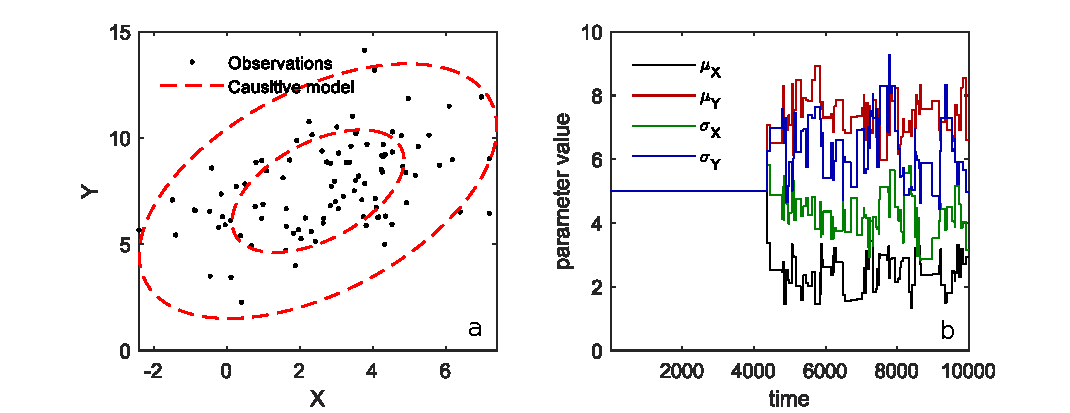
\includegraphics[scale=0.75]{init-problems.pdf}
	\caption{(a) Observed data from the underlying causitive model, whose parameters will be the inference target. (b) First 10 000 iterations of an ABC-MCMC scheme with a uniform kernel. The algorithm initially struggles to find a region of non-zero probability from a random starting position within the parameter space.}
	\label{init-qualms}
\end{figure}

%Figure of the chain becoming stuck at the beggining

While ABC-MCMC and the uniform weighting kernel $K_U$ offers improved acceptance rates compared to a rejection scheme, it is not without faults. Firstly, it can suffer from an initialisation problem, as highlighted in figure \ref{init-qualms}(b). Compounding this, the acceptance rate can rapidly decline past a certain threshold as tolerance is decreased. This is a syptom of the same problem as initialisation. Each move is either flat out rejected or is determined to be part of the posterior. This makes it prone to becoming stuck when in the tails of the posterior distribution. This is especially problematic in high-dimensional search spaces where the posterior density is an extraordinarily small volume. Ideally, if in a poor spot, the algorithm should be able to make local transitions toward an area of high probability density. However, this adjustment will involve abandoning the $K_U$. A weighting kernel which offers infinite support is needed. That is, the weight dimishes with distance, however it never reaches zero. Fortunately many functions have the required properties. In this text we favour a  weighting kernel based on the Gaussian distribution, $K_G$. This choice is advantageous as the log-distance can be evaluated for stable computation in sampling algorithms. This implementation mirrors the stable implementation of likelihood values, expanded upon in \hyperref[Box2]{Box 2}.\\

For an observed dataset $\bm{S}(\bm{y})$ and simulated dataset $\bm{S}(\bm{y^*})$, where $\bm{S} = \{S_1,\dots,S_O\}$, the Gaussian weighting kernel is computed as:
\begin{equation}
p(\bm{S}(\bm{y})|\bm{S}(\bm{y^*}),\bm{\theta}) = K_G\big(\text{d}(\bm{S}(\bm{y}),\bm{S}(\bm{y^*}))\big) \propto \prod_{i = 1}^{O} \text{exp}\Big[-\frac{1}{2}\Big(\frac{\text{d}(S_i(\bm{y}),S_i(\bm{y^*}))}{\epsilon_i}\Big)^2\Big]
\end{equation}
Figure \ref{KuVSKg-1} compares and contrasts $K_U$ and $K_G$ over the first 10 000 time steps in an ABC-MCMC algorithm targeting the parameters to a bivariate Gaussian distribution, $\bm{\theta} = \begin{bmatrix}
\bm{\mu}\ \bm{\Sigma}
\end{bmatrix}$. $K_G$ does not suffer from the same initialisation problem as $K_U$. $K_G$ also has an improved accpetance rate and better mixing when compared to $K_U$. Figure \ref{KuVSKg-2} demonstrates that with time both kernels converge to the same solution.\\

The posterior sampled in both figure \ref{KuVSKg-1} and \ref{KuVSKg-2} shows an insensitivity to $\rho$. This is a direct result of the insufficiency of the selected summary statistics for that parameter. This reinforces that while a smaller $\epsilon$ improves $\pi(\bm{\theta}|\text{d}(S(\bm{y}),S(\bm{y^*}))<\epsilon) \approx \pi(\bm{\theta}|S(\bm{y}))$, but if the summary statistics are not informative such that $\pi(\bm{\theta}|S(\bm{y})) \approx \pi(\bm{\theta}|\bm{y})$, then the house of cards falls apart. In this case the statistic $\text{cov}(X,Y)$ which should be sensitive to $\rho$, remains overwhelmed by $\sigma_X$ and $\sigma_Y$. In this case, the sample correlation, $\bar{\rho}$, would have proved a better summary statistic choice. 

\begin{figure}[H]
	\centering
	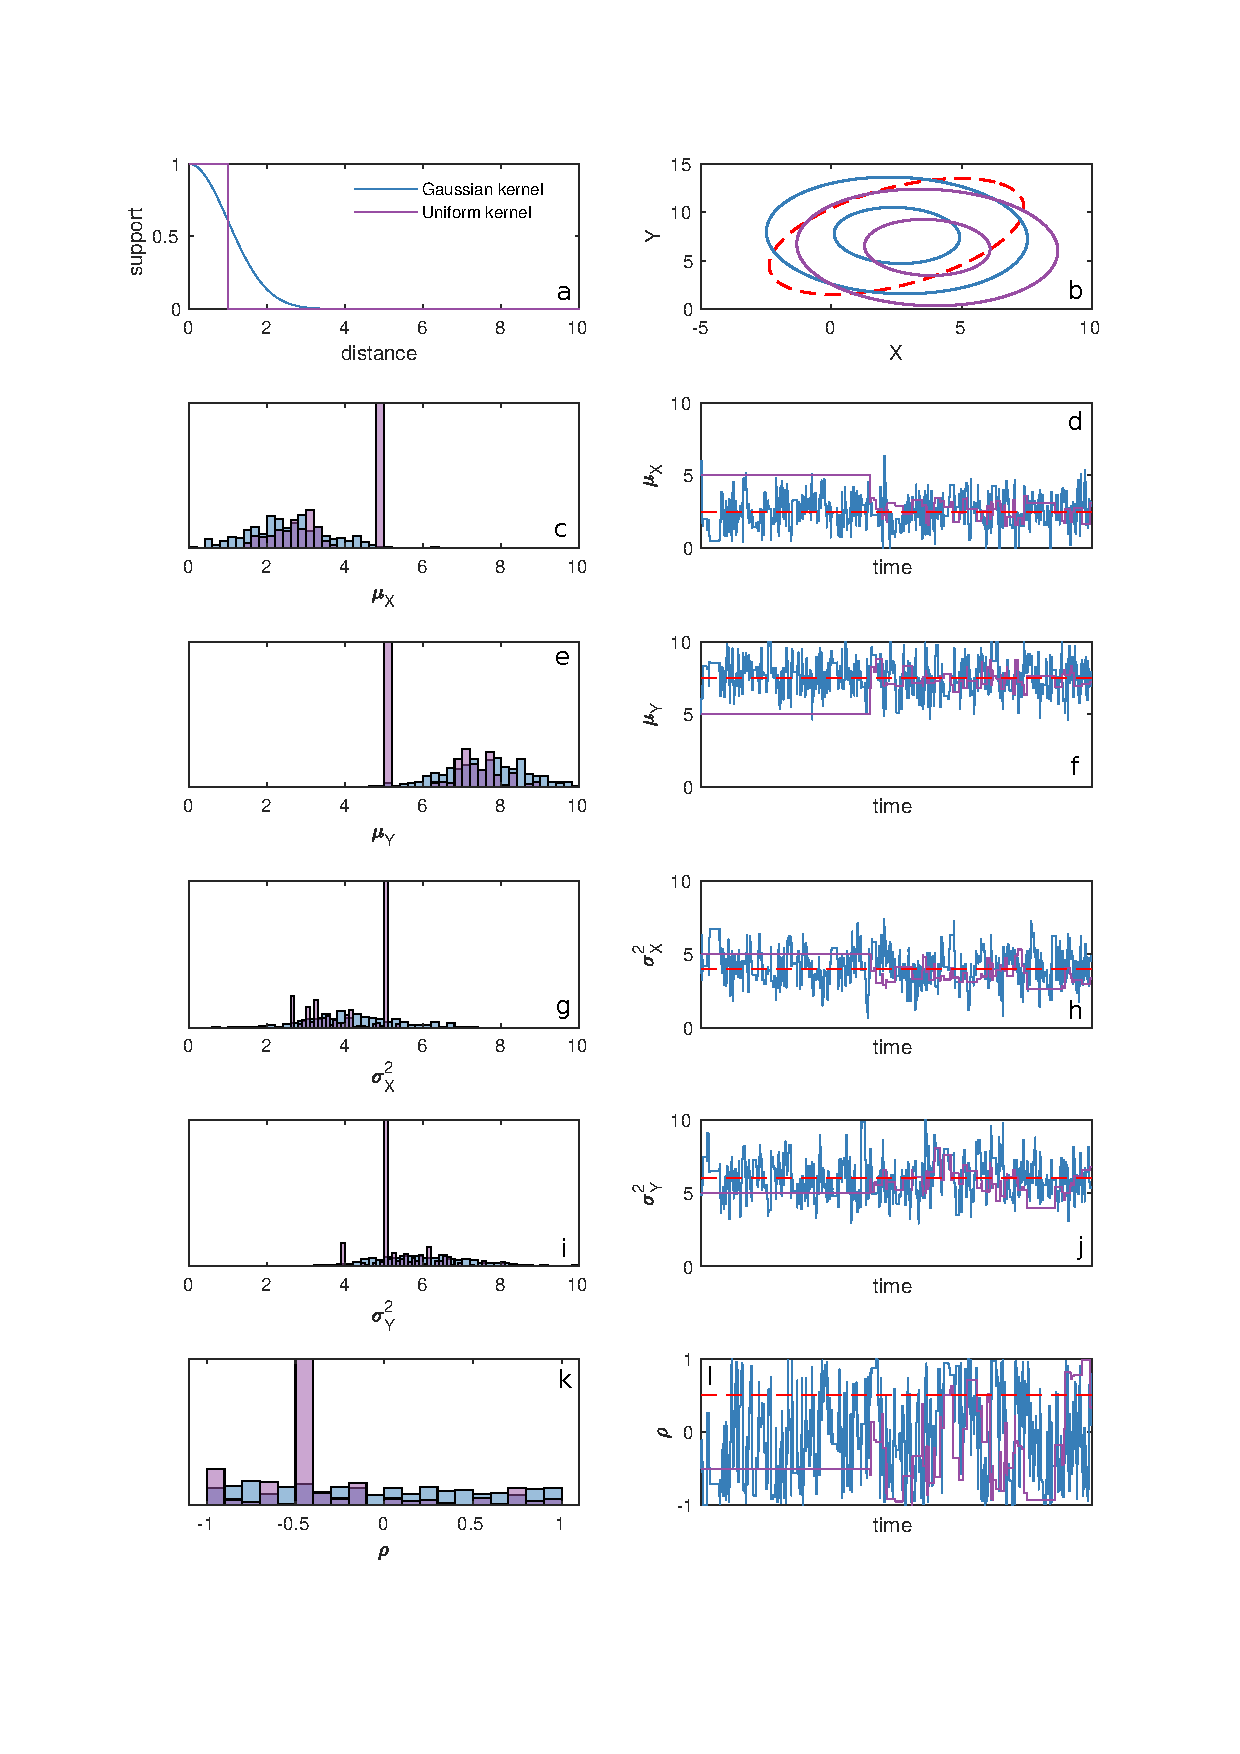
\includegraphics[scale=0.7]{BG10000.pdf}
	\caption{Comparison between the Uniform and Gaussian kernel when targeting the parameters to a Gaussian distribution with ABC-MCMC. This is the first 10 000 time steps. This demonstrates how inference based on the Gaussian kernel with infinite support, (a), overcomes the initialization problem the uniform kernel suffers from. The improved mixing and acceptance rate can be seen in the Markov chain traces, (d,f,h,j,l).}
	\label{KuVSKg-1}
\end{figure}

\begin{figure}[H]
	\centering
	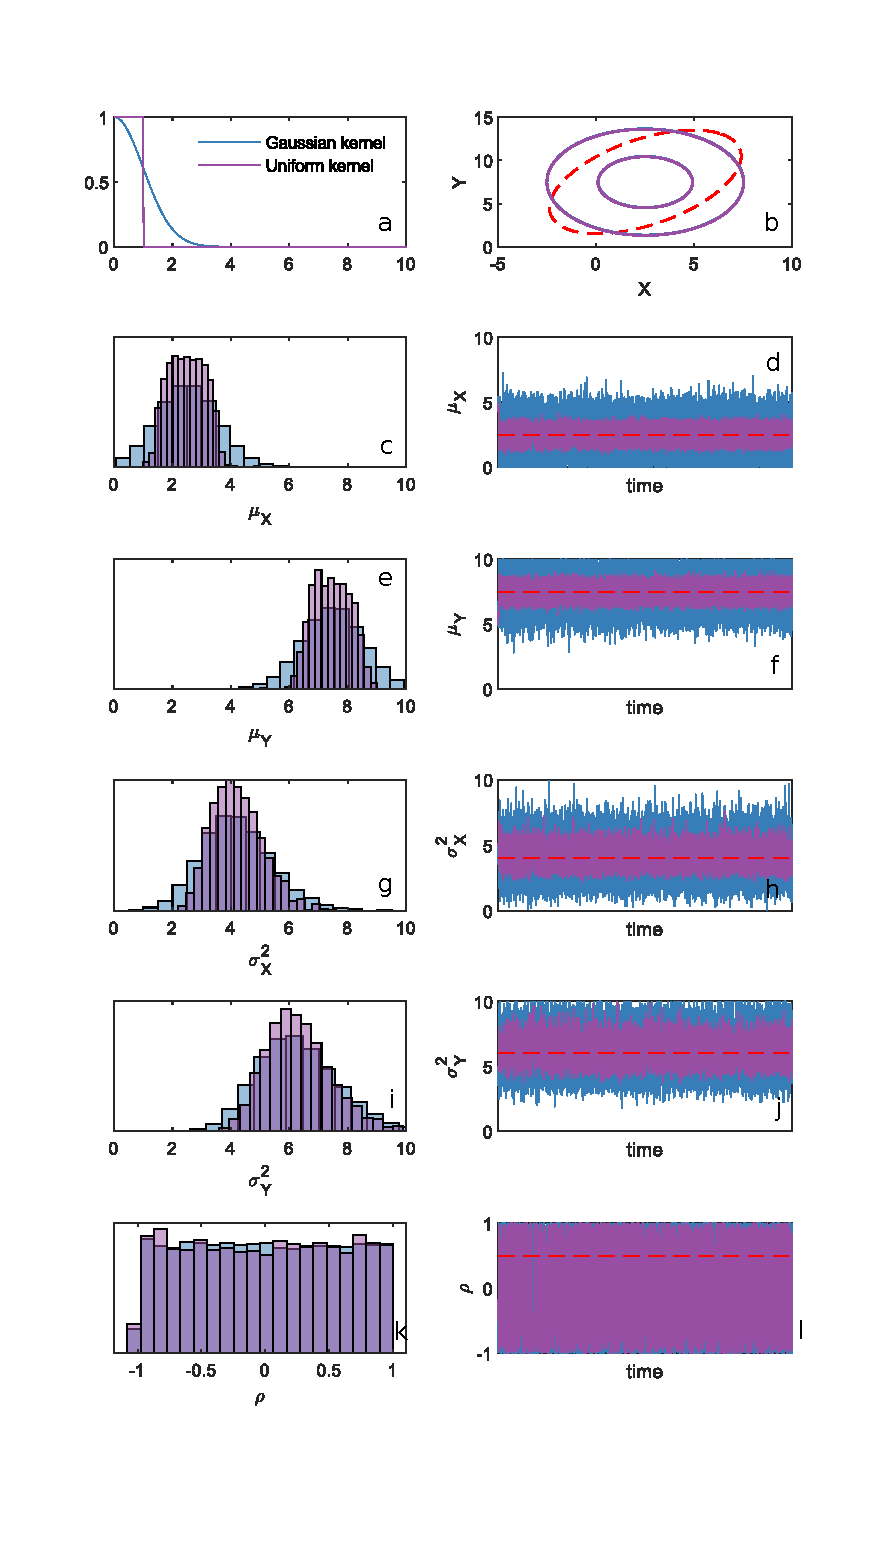
\includegraphics[scale=0.7]{BG1000000.pdf}
	\caption{Comparison between the Uniform and Gaussian kernel for 1 000 000 time steps of an ABC-MCMC algorithm. This demonstrates how the two methods converge to the same solution, in constrast to figure \ref{KuVSKg-1}. The difference in posteriors is a result of the wider support the Gaussian kernel offers compared to the equivilent uniform kernel, (a).}
	\label{KuVSKg-2}
\end{figure} 

\section{Toy problem 4: Banana distribution}

As a fourth example we desgin a more challenging problem, one for which there are no imediate and obvious summary statistics and with some degree of dimensionality. Consider we have $n = 1000$ observations from a "banana" distribution, Figure \ref{banana-data}. To define the banana distribution, we start with a 2-dimensional Gaussian distribution:
\begin{equation}
\begin{bmatrix}
x\ y
\end{bmatrix}=\mathcal{N}(\bm{\mu},\bm{\Sigma}),\ \bm{\mu} = \begin{bmatrix}
\mu_X\ \mu_Y
\end{bmatrix}^T,\ \bm{\Sigma} = \begin{bmatrix}
\sigma^2_X & \rho\sigma_X\sigma_Y\\
\rho\sigma_X\sigma_Y & \sigma^2_Y
\end{bmatrix} 
\label{gauss-banana}
\end{equation}
The Gaussian co-ordinates $x$ and $y$ are then twisted to produce a more nonlinear target, $X$ and $Y$, using:
\begin{equation}
X = b_1x
\label{x-banana}
\end{equation}
\begin{equation}
Y = y/a-b_2(b_1^2x^2+b_1^2)
\label{y-banana}
\end{equation}
In total the parameters which define this model are $\bm{\mu}$, $\bm{\Sigma}$ and the banana parameters $\begin{bmatrix}
b_1\ b_2
\end{bmatrix}$. Here the unknown target parameters are $\bm{\mu} = \begin{bmatrix}
0\ 0
\end{bmatrix}^T$,
$\bm{\Sigma} = \begin{bmatrix}
\sigma^2_X & \rho\sigma_X\sigma_Y\\
\rho\sigma_X\sigma_Y & \sigma^2_Y
\end{bmatrix}$ while $\begin{bmatrix}
b_1\ b_2
\end{bmatrix}$ = $\begin{bmatrix}
1\ 1
\end{bmatrix}$. 

\begin{figure}[H]
\centering
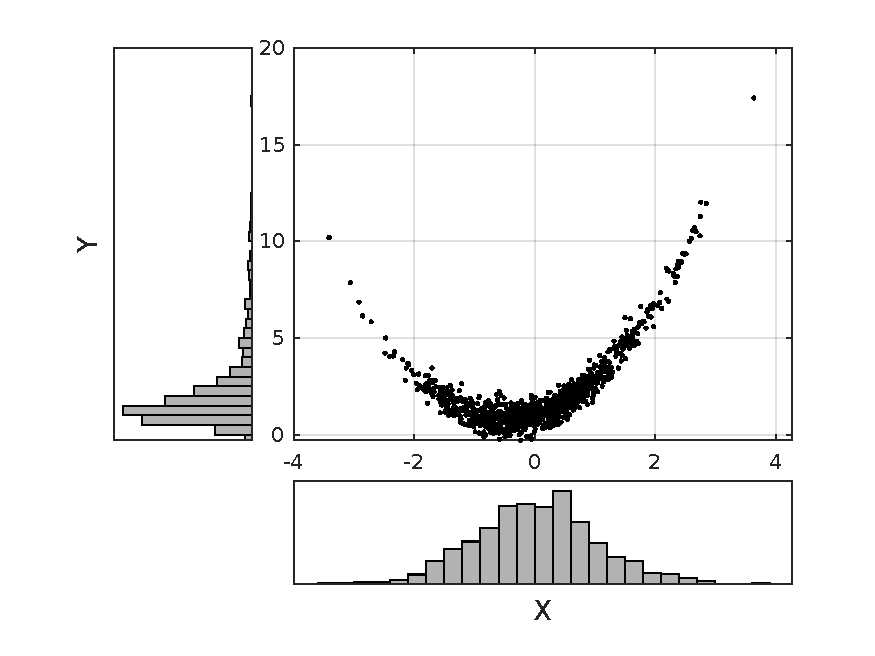
\includegraphics[scale=1]{banana-data.pdf}
\caption{$n = 1000$ observations from the "banana" distribution, analytically defined by equations \ref{gauss-banana}, \ref{x-banana}, \ref{y-banana}. 
This problem is more challenging as there is no immediately apparent sufficient statistics to facilite ABC estimation of the unknown parameters.}
\label{banana-data}
\end{figure}

To proceed with ABC inference under this model we must define a set of reasonably sufficient statistics. In the previous examples it has been possible to use the sample values for each of the unknown parameters, however, here this proved to be insufficient in a trial run. In the ABC literature summary statistic selection is the focus of technique development and active research. \citet{Blum2013} and \citet{Prangle2017} offer comprehensive reveiws of this research area. For this example we heed the advice of \citet{Wood2010}. The statsitics have the same role in ABC as the data do in a traditional likelihood. Hence, there is no need for certain statistics to relate to specific parameters any more than there is the need for certain data points to relate to specific parameters. The key is in indenitifying a set of statistics which is senstitive to the scientificaly important and repeatable features of the data, and insensitive to the transient noisey components. \citet{Wood2010} identifies marginal distribution statistics as being a useful first step. The marginal distribution for our banana observations, $X$ and $Y$, are plotted in figure \ref{banana-data}. Here we can see $X$ appears as a regular Gaussian distribution, while $Y$ appears as a skewed-Gaussian distribution. This motivates the choice of marginal statistics for $X$ as the sample mean, $\bar{\mu_X}$, and sample standard deviation, $\bar{\sigma_X}$. While marginal statistics for $Y$ are sample skewness $\bar{\gamma_Y}$, as well as $\bar{\mu_Y}$ and $\bar{\sigma_Y}$. However, this does not capture the "shape" of the joint distribution in 2D dimensions. To capture the bananity of the joint distribution we fit a second degree polynomial to the data, $Y = aX^2 + bX + c$. The co-effecient values $a$, $b$ and $c$ are then used as the summary statistics. For this example we consider this set, $\begin{bmatrix}
\bar{\mu_X}\ \bar{\sigma_X}\ \bar{\gamma_Y}\ \bar{\mu_Y}\ \bar{\sigma_Y}\ a\ b\ c
\end{bmatrix}^T$, to constitute reasonably sufficent summary statistics for the banana distribution. However, these are not perfect, and the effect of using them will be the introduction of some degree of bias into the ABC posterior. \\



% Introduce scaling considerations
In our applications so far the distance metric has been a vector composed of the absolute distance between observed and simulated summary statistics, hence:
\begin{equation}
\text{d}_i(S_i(\bm{y}),S_i(\bm{y^*})) = |S_i(\bm{y})-S_i(\bm{y^*})|
\end{equation}
is the marginal fit for a given statistic. In our examples it has not been necessary to consider the scale the chosen statistics vary over and their sensitivity to the unknown parameters. For the most part all statistics have been equally sensitive and varied over a similar scale. Under a rejection scheme where all simulations and distances can be computed before the rejection step, it is straight forward to normalize the distances by the scale they vary over. However, it is not clear how to best account for this scale and sensitivity when using ABC-MCMC. One solution would be to use variable tolerances which account for this scale and sensitivity, establishing $\epsilon = \{\epsilon_1,\dots,\epsilon_O\}$. However, this is not a user friendly solution to the issue of scale as implementation would invariably involve many repitions as $\epsilon$ is tuned. Other authors, \citet{Ratmann2010}, have normalised the marginal weighting term, the weight for each individual statistic, to one. I attempt a transformation in a similar spirit by approximating a term $\sigma_{S_i}$ which will normalize the spread of distance for each statistic to one. In algorithms distance is replaced by a normalized-distance:
\begin{equation}
\hat{d_i}(S_i(\bm{y}),S_i(\bm{y^*})) =  \frac{|S_i(\bm{y})-S_i(\bm{y^*})|}{\sigma_{S_i}}
\end{equation}

% Computing the normalization term
A good sampling algorithm would temper $\bm{\sigma_S} = \{\sigma_{S_1},\dots,\sigma_{S_O}\}$ on the fly. Without such an algorithm $\bm{\sigma_S}$ must be predefined. Here we favour a Monte Carlo approximation based on $k > 10\ 000$ simulations from the prior and given the observed data. A marginal term $\sigma_{S_i}$ is then defined as the sample standard deviation of the distance between the simulated summary statistic and the observed summary statistic:
\begin{equation}
\sigma_{S_i} = \sqrt{\frac{\sum_{i = 1}^{k}(\text{d}_i)^2}{k-1}}
\end{equation}
This does not preclude varying $\epsilon$, however, it does ensure that each marginal $\epsilon_i$ is of a simular magnitude. \\



Figure \ref{MH-banana} shows the results of an ABC-MCMC algorithm targeting the banana distribution. This leverages a Gaussian kernel, summary statistics as described and uses a normalized distance metric. For this problem only the Gaussian parameters, $\bm{\mu}$ and $\bm{\Sigma}$ are unknown.\\

% Insert banana problem solved w/ MCMC + MLE plot
\begin{figure}[H]
	\centering
	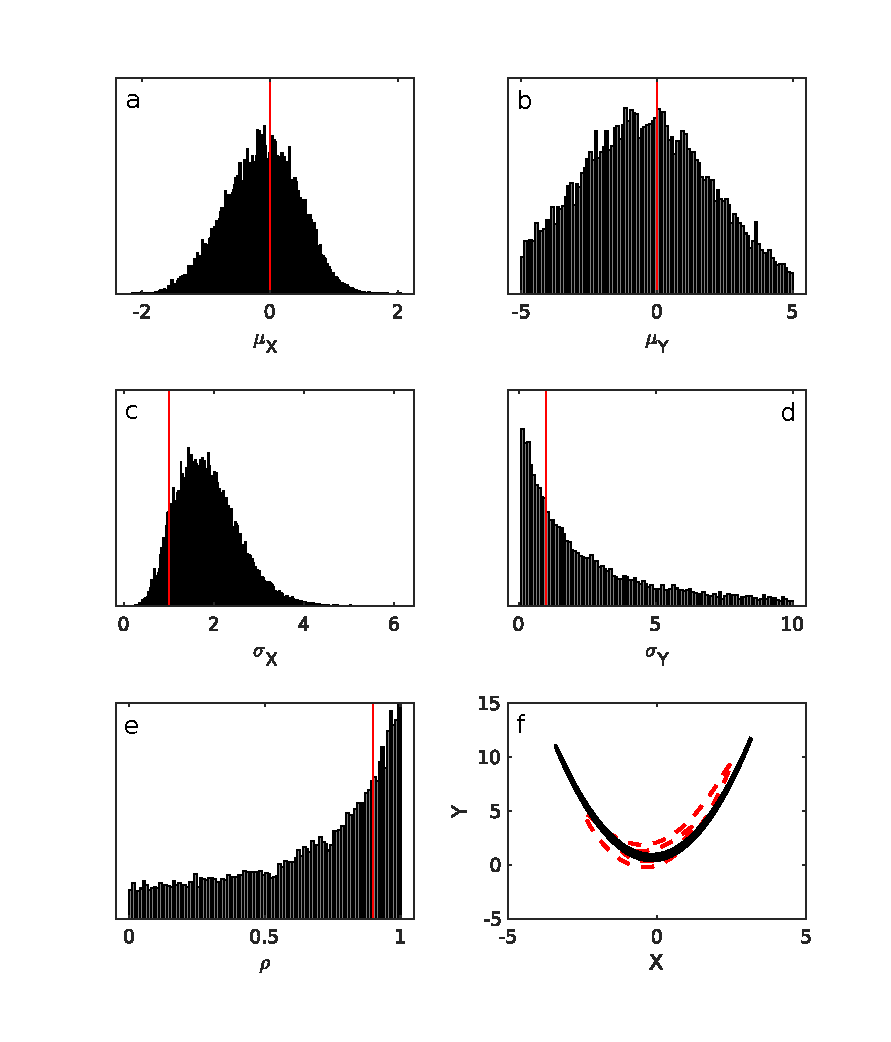
\includegraphics[scale=1.1]{MH-Banana-1mil.pdf}
	\caption{The marginal posterior distributions for banana parameter inference, as well as the median posterior model (f), in black, compared to the original model, red dashed lines. Red lines mark the true parameter values on the marginal posterior plots. I justify the legitimacy of extracting the median marginal model as there are limited correlations between the unknown parameters.}
	\label{MH-banana}
\end{figure}

Throughout this chapter, I plot the median marginal posterior model. That is, the model which is defined by taking the median of the Markov chain for each individual parameter. One example is figure \ref{MH-banana}(f), here the red dashed lines mark the 50\% and 95\% confidence intervals of the model the data was generated from, while the solid black lines mark the 50\% and 95\% confidence intervals of the median marginal posterior model. Often the marginal parameter densities are considered as the principal result from Bayesian parameter inference. However, the marginal posterior distributions hide correlations between parameter which may be present in the joint posterior, which is the distribution the Markov chain sampled. If there are correlations between parameters then a given parameters uncertainty will appear greater in the marginal distribution. To keep inference honest I plot the correlations between each parameter, figure \ref{correlation-plot}, from the Markov chain generated in figure \ref{MH-banana}. As can be seen there are limited correlations between parameters. As a result, extracting the marginal median is an accurate representation of the median model under the joint distribtuion. An accurate estimate of the uncertainty can also be found by taking the marginal standard deviation. If there was significant uncertainty between some $\theta_1$ and $\theta_2$ then it would not make sense to evaluate $\theta_2$ marginally with $\theta_2 = \mu \pm \sigma$. Instead $\sigma$ would need to be evaluated with respect to a given value for $\theta_1$, in order to have a proper understanding of the uncertainty in $\theta_2$. 

% Insert correlation plot of 5 pars to justify taking the MLE
\begin{figure}[H]
	\centering
	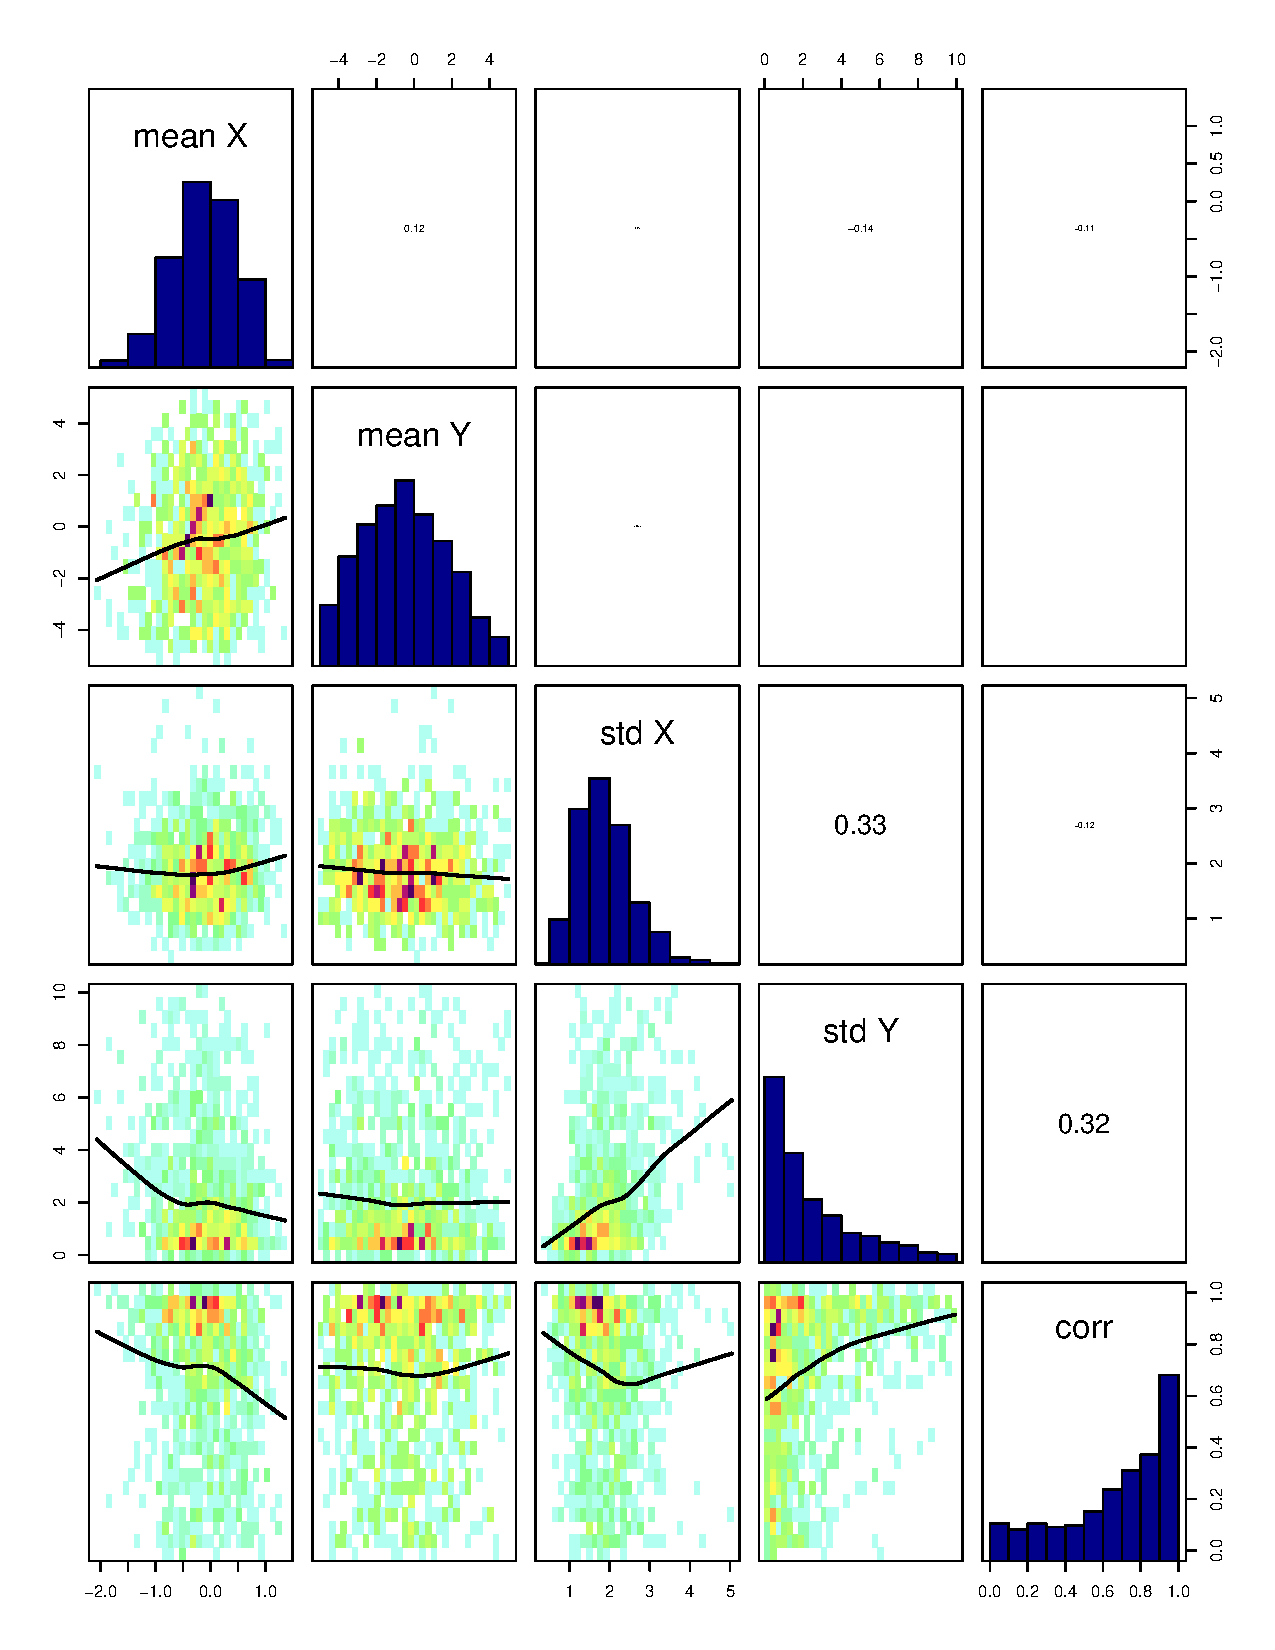
\includegraphics[scale=0.6]{correlation-plot.pdf}
	\caption{Correlation plot for the Markov chain in figure \ref{MH-banana}. There is limited correlation between the parameters. This is used as justification for plotting statistics of the marginal posterior as representative of the joint posterior.}
	\label{correlation-plot}
\end{figure}


The performance of our MCMC algorithm as described by algorithm \ref{ABC-MCMC} depends on the users ability to choose a suitable proposal distribution $q(\cdot,\cdot)$. If we limit the proposal distribution to a multivariate Gaussian distribution, then we must choose a suitable covariance matrix for it. If the variance for each parameter is too large then the probability of accepting a candidate move will be low, as each step will be erratic and far from the current location. Consider that as the variance for $q(\cdot,\cdot) \rightarrow \infty$ we effectively have a Monte Carlo scheme. However, if the variance is too small then the acceptance rate will be very good but algorithm will fail to explore the full parameter space. Hence there is a balance encoded in the selection of the proposal distribution. We desire both a reasonable acceptance and a good exploration of the parameter space. In this way we select a proposal distribution which suits the underlying target distribution. Generally it is simplest to leave the off-diagonal terms in the proposal distribution's covariance matrix, the correlations between parameters, unconsidered.\\

However, such a system is not ideal. Selecting an optimal proposal distribution is non-trivial problem. Here we can turn to theoretical developments to guide a better proposal distribution. \citet{Gelman1996} show that when the target distribution is Gaussian, an efficient sampler can be constructed by scaling the proposal covariance to $2.4^2/d$, where $d$ is the number of unknown parameters. In the previous sections it has been best to ignore the correlations between parameters. However, these correlations can be important to consider, if there are strong parameter correlations in the posterior then sampling success can be weakened by leaving these unconsidered, especially in a high dimensional space and for nonlinear problems. Indentifying these correlations ahead of time and designing a pre-defined proposal is challenging. Ideally the algorithm should be able to learn about the posterior on the fly, and if there are correlations betweeen parameters, adjust accordingly. With this in mind \citet{haario2001} developed Adaptive Metropolis (AM). AM tunes the proposal distribution to the posterior distribution by using the history of the chain generated so far. After some designated time, $t$, the covariance matrix of the proposal distribution, $\bm{\Sigma_q}$, is set to the covariance of the Markov chain so far. 
\begin{equation}
\bm{\Sigma_q} = \text{cov}(\bm{\theta}_1,\dots,\bm{\theta}_t)s_{AM} + I\upsilon
\end{equation}
Where $s_{AM}$ is the scaling factor, generally $2.4^2/d$, and $\upsilon$ is a small positive which prevents the covariance from becoming singular. AM sampler efficiency is compared to MH in table \ref{sampling-method-comparison}.\\

Figure \ref{AM-demonstration} plots the effect AM has on a sub-optimal choice for a proposal distribution.\\

Throughout this text we use a 4-stage adaptive scheme over the length of the chain. Figure \ref{4-stage-am} plots this scheme. With this in mind, Figure \ref{AM-demonstration} plots the proposal distribution before the first adaption, red, and after the 4th adaption, blue. \\
\linebreak
\linebreak
\linebreak

\begin{figure}[h]
%\vspace{2cm}
\begin{minipage}{1.0\linewidth}
\centering
    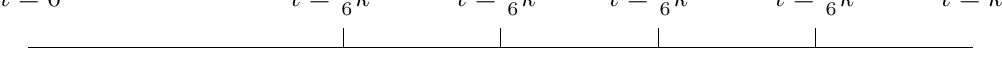
\begin{tikzpicture}
	\draw (0,0) -- (12,0);
	\draw (4,0) -- (4,0.25);
	\draw (6,0) -- (6,0.25);
	\draw (8,0) -- (8,0.25);
	\draw (10,0) -- (10,0.25);

	\put(-10,15){$t = 0$}
	\put(95,15){$t = \frac{2}{6}k$}
	\put(155,15){$t = \frac{3}{6}k$}
	\put(210,15){$t = \frac{4}{6}k$}
	\put(270,15){$t = \frac{5}{6}k$}
	\put(330,15){$t=k$}

	\put(108,50){$1^{st}$}
	\put(95,40){$adaption$}
	\put(163,40){$2^{nd}$}
	\put(220,40){$3^{rd}$}
	\put(277,40){$4^{th}$}
    \end{tikzpicture}
\end{minipage}

\caption{4-stage adaptive scheme for a Markov chain of length $k$}
\label{4-stage-am}
\end{figure}

\begin{figure}[H]
	\centering
	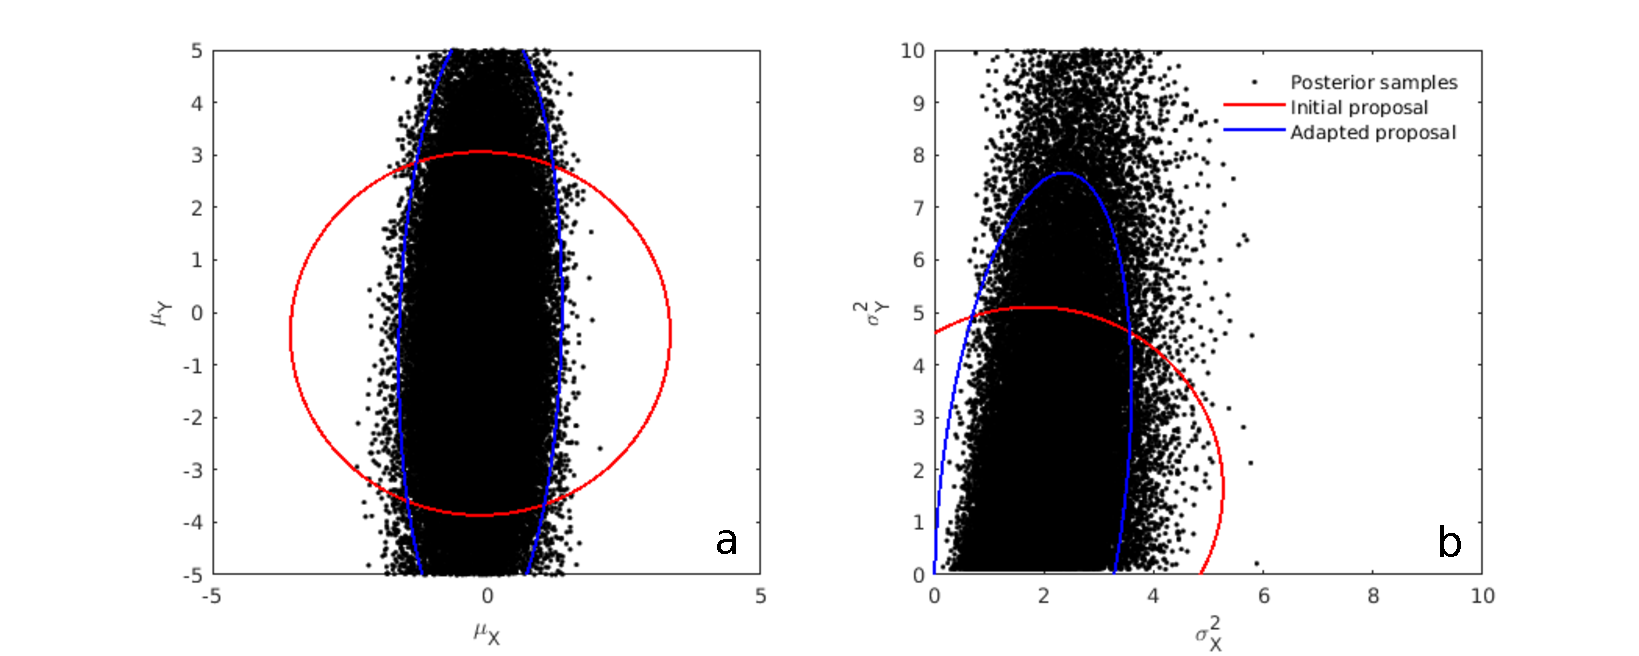
\includegraphics[scale=0.45]{Am-demonstration.pdf}
	\caption{Adapted proposal distribution compared to a suboptimal initial proposal. This suboptimal choice was the proposal distribution of the MCMC algorithm in figure \ref{MH-banana}.}
	\label{AM-demonstration}
\end{figure}

Delayed Rejection (DR) can also be implmented to improve sampling efficiency \citep{Mira2001}. Under DR, when a proposed move is rejected, instead of advancing a time step and retaining the same position, another proposed candidate move is considered. The acceptance probability of the second proposal differs from the MH acceptance probability in order to retain time reversibility of the Markov chain, ensuring that the chain converges to the desired stationary distribution. When a Markov chain remains in the same position over time, the estimates obtained by averaging along the chain become less accurate. Increases to the autocorrelation of the chain increase the variance of estimates based on the chain \citep{Mira2001}. In this way DR gives more reliable estimates than a standard MH algorithm. A two-stage DR algorithm, as is applied in this text, operates as follows. \\

At the first stage the acceptance probability is the Metroplis-Hastings acceptance probability:
\begin{equation}
	\alpha_1(\theta,\theta^*) = \text{min}\bigg\{1,\frac{\pi(\theta^*)q_1(\theta^*,\theta)}{\pi(\theta)q_1(\theta,\theta^*)} \bigg\}
\end{equation}
where $\pi$ is the target distribution of the algorithm and $q_1$ is the proposal distribution. If the proposed move to $\theta^*$ is rejected then a second candidate move, $\theta^{**}$, can be considered from the second proposal distribution $q_2$. The acceptance probability for $\theta^{**}$ is:
\begin{equation}
	\alpha_2(\theta,\theta^*,\theta^{**}) = \text{min}\bigg\{1,\frac{\pi(\theta^{**})q_1(\theta^{**},\theta)q_2(\theta^{**},\theta^*,\theta)[1-\alpha_1(\theta^{**},\theta^*)]}{\pi(\theta)q_1(\theta,\theta^*)q_2(\theta,\theta^*,\theta^{**})[1-\alpha_1(\theta,\theta^*)]} \bigg\}
\end{equation}
Here I limit implementation to a two-stage DR scheme and use a $q_2$ with a smaller covariance matrix. $q_1$ is downscaled to give $q_2$ by the relation, $q_2 = q_1/s_{DR}$. DR is compared to MH and AM in table \ref{sampling-method-comparison}.\\

Both Adaptive Metropolis and Delayed Rejection can be implemented together to give a Delayed Rejection Adaptove Metropolis scheme \citep{Laine2008}. There are many implementation possibilities given the mixing of AM and DR. Here a straight forward implementation is favoured, as in \citet{Laine2008}, which retains the principal advantages of each method to give an efficient adaptive algorithm.    The first stage proposal is adapted to the chain generated so far, and one scaled down second stage proposal is considered. The second stage proposal inherits the adapted covariance matrix of the first stage proposal, only the variances are down scaled. DRAM is compared to MH, AM and DR in table \ref{sampling-method-comparison}.\\

When running a 'one-size fits all' generic MCMC algorithm, the standard procedure is to propose a candidate move which updates each and every parameter value. If we are at the position $\bm{\theta_{t-1}}$ in the parameter space, then the proposal distribution suggests a candidate move:
\begin{equation}
	\bm{\theta_{t}} = \mathcal{N}(\bm{\theta_{t-1}},\bm{\Sigma_q})
\end{equation}
However, this is not the only option. Another generic choice is to update a single parameter per time step. Much like the variance of $\bm{\Sigma_q}$, there is a trade-off between acceptance rate and speed of parameter space exploration encoded into this decision. Table \ref{sampling-method-comparison} compares the acceptance rate of a MH algorithm where all parameters are updated at once, and an MH algorithm where a single parameter is updated per time step. A significant increase in acceptance rate is made through this change. There is also a third option. At each time step a sub-set of parameters are updated. This is referred to as blocking. When parameters that are correlated are updated as a block together, sampler performance is increased relative to updating each dimension independantly \citep{Turek2017}. However, implementing effective parameter blocking is not user friendly and requires problem specific implementation. 

\begin{table}[H]
	\centering
	\begin{tabular}{|c|c|}
	\hline
	Sampling method & Acceptance rate (\%) \\
	\hline
	Metropolis-Hastings (MH) & 5.22\% \\
	\hline
	Adaptive Metropolis (AM) & 10.63\% \\
	\hline
	Delayed Rejection (DR) & 28.35\% \\
	\hline
	Delayed Rejection Adaptive Metropolis (DRAM) & 36.44\% \\
	\hline
	Single parameter update & 35.83\% \\
	\hline
	\end{tabular}
	\caption{Comparison of sampler efficiency for the banana parameter estimation problem. The sampled posterior is the same for each method. The AM acceptance rate is taken for samples after the 4th adaption. DRAM acceptance rate is taken over the full length of the chain. Each chain is of length $t = $ 900 000.}
	\label{sampling-method-comparison}
\end{table}

While ABC targets the underlying parameters to the banana distribution, there is also access to the probability density of the causitive model. With access to the causitive models probability in $X-Y$ space it is possible to run a Markov chain to discover the distribution. Figure \ref{Analytical-banana}(a) plots a Markov chain with the stationary distribution of the causitive model, black dots, as well as the 50\% and 95\% confidence intervals of the causitive model. The markov chain can be used for kernel density estimation of the causitive model, figure \ref{Analytical-banana}(b). With this in mind it is possible to compare the estimation of the causitive model with ABC and under access to the analytical probability density. Figure \ref{the-comparison} compares the estimation of the causitive model based on a standard MH algorithm (a), AM (b), DR (c), DRAM (d), and ABC-MH (e), ABC-AM (f), ABC-DR (g), ABC-DRAM (h). 

\begin{figure}[H]
\centering
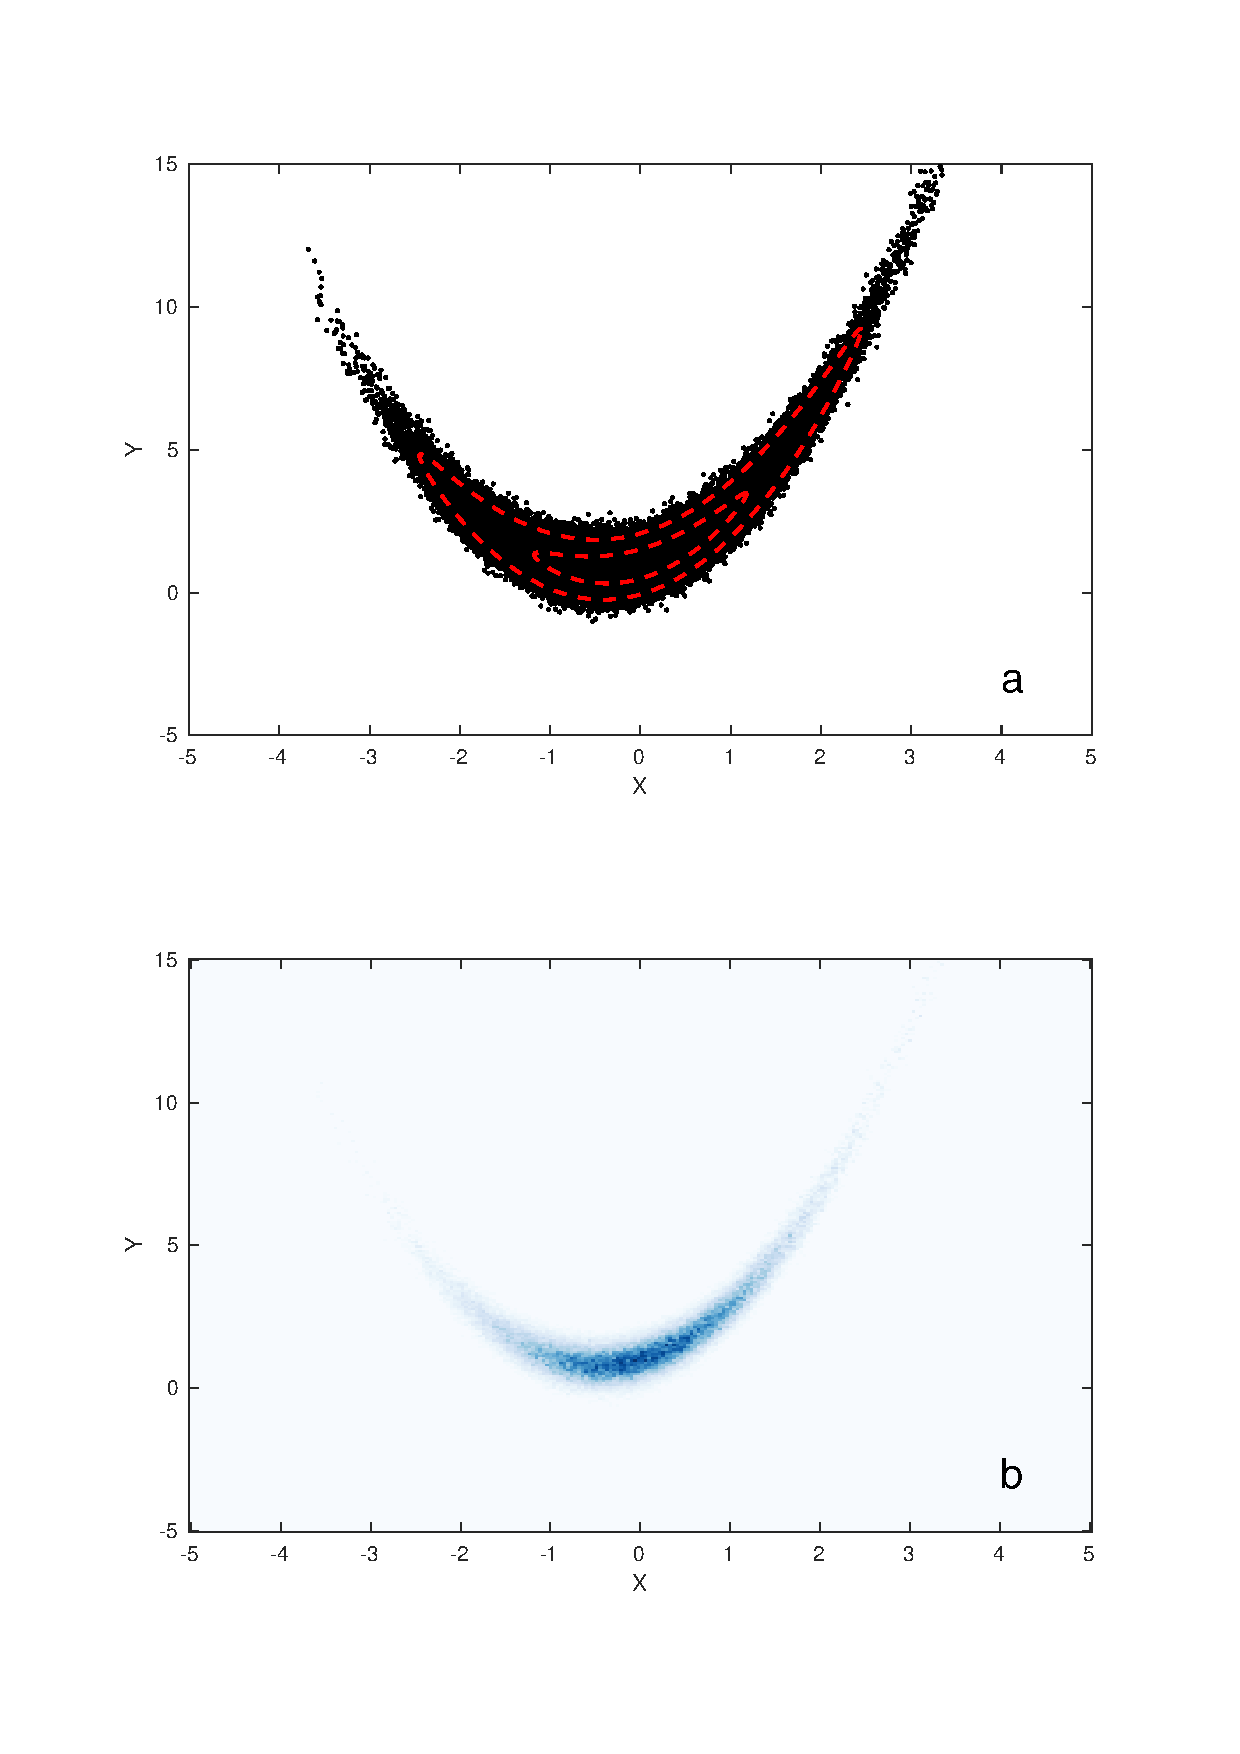
\includegraphics[scale=0.45]{MH-banana.pdf}
\caption{A Metropolis-Hastings algorithm sampling the causitive model. (a) The MCMC samples, black dots, to the causitive model. Red dashed lines mark the 50\% and 95\% confidence intervals of the causitive model. (b) kernel density estimation based on the MCMC samples. Kernel density estimation in 2d is based on the diffusion algorithm of \citet{Botev2010}.}
\label{Analytical-banana}
\end{figure}

\begin{figure}[H]
\centering
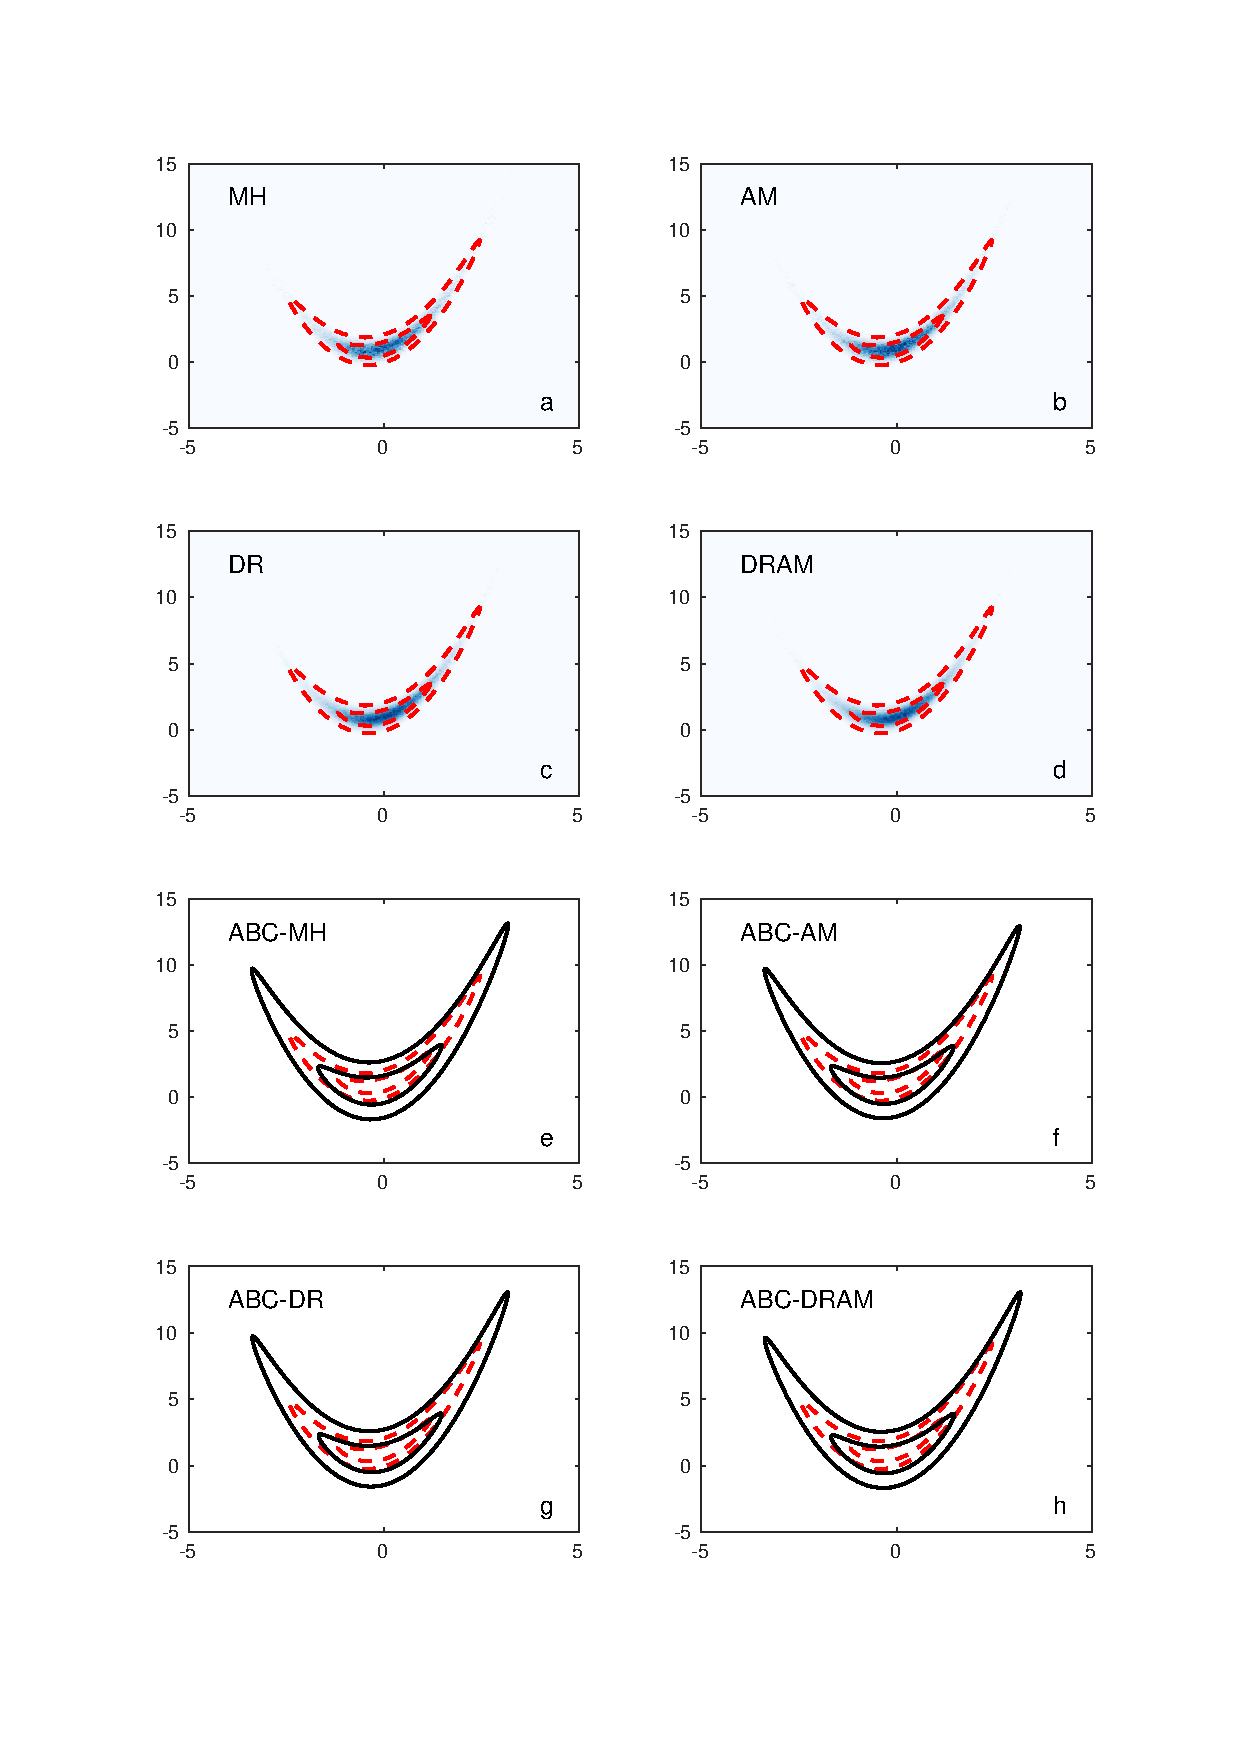
\includegraphics[scale=0.8]{Analytical-vs-ABC.pdf}
\caption{Comparison of estimation of the causitive banana model based on access to the analytical formula (a,b,c,d) and no access to the analytical formula (e,f,g,h), simply simulation from the model.}
\label{the-comparison}
\end{figure}

Throughout this example a strong trend has emerged. The acceptance rate of a Markoc chain based algorithm targeting the ABC posterior is strongly tied to the tolerance. This shows the effect of tolerance in a rejection scheme is persistent, and generalizes to more advanced samplers. Increasing the tolerance increases the acceptance rate, while decreasing the tolerance decreases the acceptance rate. With this in mind, the improvments to the acceptance rate of ABC-MCMC offered by AM, DR, single parameter updates and blocking are very important for sampling the most accurate posterior possible. With each improvement to acceptance rate the tolerance can be lowered while still remaining in the realm of reasonable sampler efficiency, around 10-30\% acceptance rate. So far all comparisons have been done using a tolerance $\epsilon =\begin{bmatrix}
0.5\ 0.5\ 0.5\ 0.5\ 0.5\ 0.1\ 0.5\ 0.5
\end{bmatrix}^T$ 
for the statistic set $\begin{bmatrix}
\bar{\mu_X}\ \bar{\sigma_X}\ \bar{\gamma_Y}\ \bar{\mu_Y}\ \bar{\sigma_Y}\ a\ b\ c
\end{bmatrix}^T$. This tolerance is used to keep ABC-MH, the worst performing sampler, computationally feasible. However, using ABC-DRAM with single parameter updates it is possible to lower the tolerance to 
$\epsilon = \begin{bmatrix}
0.125\ 0.125\ 0.125\ 0.125\ 0.125\ 0.025\ 0.125\ 0.125
\end{bmatrix}^T$
while still remaining within the limits of computational feasability. Figure \ref{best-banana} plots this scenario. With ABC-DRAM and single parameter updates the acceptance rate is ~7\% under this tolerance. While ABC-MCMC sampling, with all parameter updates, becomes computationally infeasable with an acceptance rate <0.25\%.

\begin{figure}[H]
\centering
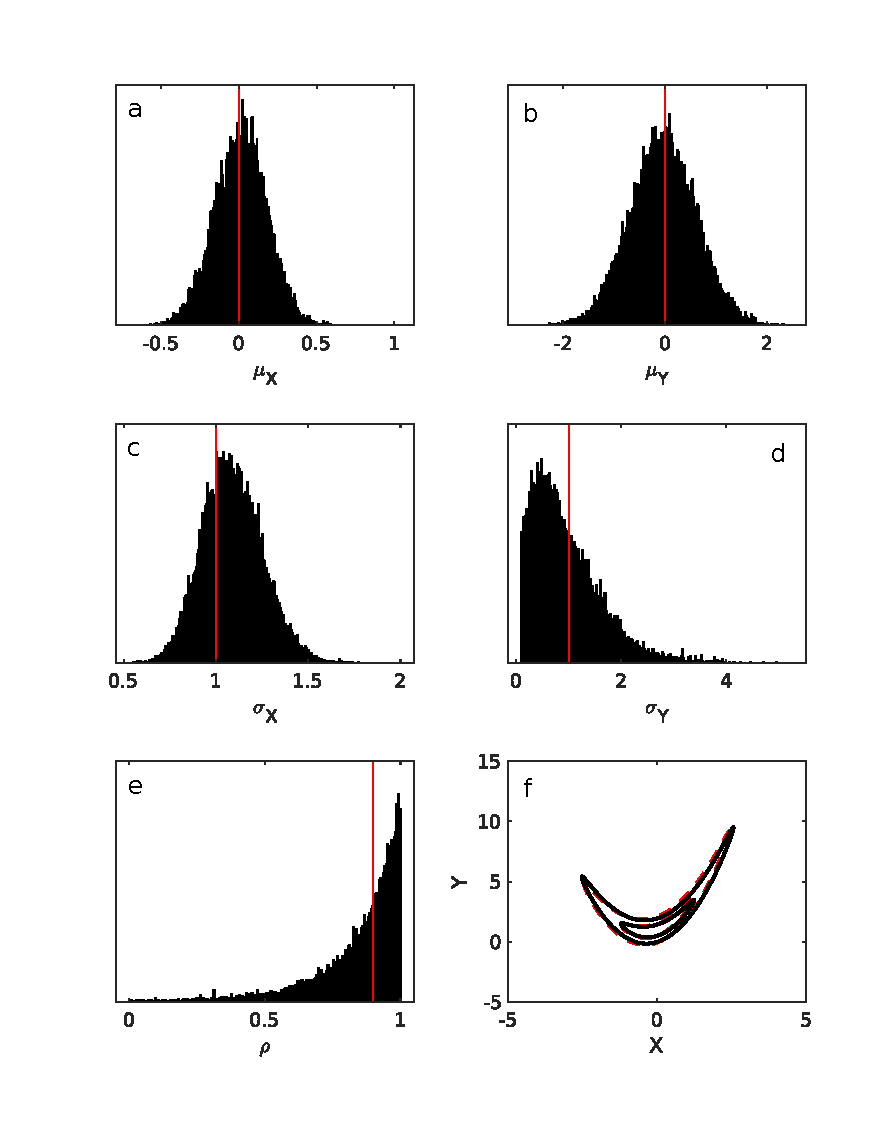
\includegraphics[scale=1.1]{DRAM-blocked-banana.pdf}
\caption{Banana parameter estimation based on ABC-DRAM with single parameter updates. The tolerance is lowered, see text for tolerance values. By lowering the tolerance inference is more accurate. Compared to \ref{MH-banana} the marginal posteriors are more tightly clustered around the true solution and the median marginal model, black lines of (f) fit the causitive model, red dashed lines, far better.}
\label{best-banana}
\end{figure}